\documentclass[aspectratio=46, dvipdfmx, 10pt, t]{beamer} % aspectratio=43, 149, 169

% Style File

\usepackage{here, amsmath, latexsym, amssymb, bm, ascmac, mathtools, multicol, tcolorbox, subfig}
\usepackage{multirow}
\usepackage{graphicx}
\usepackage{comment}
\usepackage{amsmath}
\usepackage{atbegshi} % しおりの文字化け解消
\usepackage{xcolor}
\usepackage{xspace}
\usepackage{hyperref}

\usetheme{Luebeck}                % デザインの選択(省略可)
\usecolortheme{orchid}            % カラーテーマの選択(省略可)


% -------------------
% フォント
% -------------------
%usefonttheme{professionalfonts} % フォントテーマの選択(省略可)
%\usefonttheme{structuresmallcapsserif}
\usefonttheme{default}

\useinnertheme{circles}           % フレーム内のテーマの選択(省略可)
%\useoutertheme{infolines}        % フレーム外側のテーマの選択(省略可)
\setbeamertemplate{headline}{}    % ヘッダーを表示しない

% -------------------
% タイトルページ
% -------------------
\makeatletter
\defbeamertemplate*{title page}{supdefault}[1][]
{
  \vbox{}
  \vfill
  \begingroup
    \centering

    \begin{beamercolorbox}[sep=25pt,left,#1]{title}
      \usebeamerfont{title}
        \vskip0.25em%
      \vspace{15mm}
      \textbf{\inserttitle}\par%
      \vspace{2mm}
      \ifx\insertsubtitle\@empty\relax%
      \else%
        {\usebeamerfont{subtitle}\usebeamercolor[fg]{subtitle}\insertsubtitle\par}%
      \fi%
    \end{beamercolorbox}%

    \vskip1em\par

    \begin{beamercolorbox}[sep=8pt,left,#1]{author}
      \hspace{5mm}
      \usebeamerfont{author}\insertauthor
      \vspace{-5mm}
    \end{beamercolorbox}

    \begin{beamercolorbox}[sep=8pt,left,#1]{institute}
      \hspace{5mm}
      \vspace{-5mm}
      \usebeamerfont{institute}\insertinstitute
    \end{beamercolorbox}

    \begin{beamercolorbox}[sep=8pt,left,#1]{date}
      \hspace{5mm}
      \vspace{-5mm}
      \usebeamerfont{date}\insertdate
    \end{beamercolorbox}\vskip0.5em

    {\usebeamercolor[fg]{titlegraphic}\inserttitlegraphic\par}
  \endgroup
  \vfill
}
\setbeamertemplate{title page}[supdefault][colsep=-4bp,rounded=true,shadow=\beamer@themerounded@shadow]
\setbeamercolor{title}{fg=black}
\makeatother

% -------------------
% フッター
% -------------------
\setbeamertemplate{footline}[frame number] %スライド番号のみ表示
\setbeamercolor{section in head/foot}{fg=white, bg=darkgray}    %フッターの文字色、背景色
\setbeamerfont{footline}{size=\fontsize{5}{7}\selectfont}

\setbeamertemplate{footline}{
  % フッターの縁装飾
  \begin{beamercolorbox}[ht=5ex,leftskip=1.4cm,rightskip=.3cm]{author in head/foot} 
    \vspace{0.05cm}\hspace{-1cm}
    {\footnotesize \insertauthor} \hspace{3.2cm}  % 著者名
    {\footnotesize \insertdate}   \hspace{4cm}  % 日付
    {\footnotesize \insertframenumber}            % ページ番号
  \end{beamercolorbox}
}

% -------------------
% フレームの設定
% -------------------
\setbeamersize{text margin left=0.5mm,text margin right=1em}
\setbeamercolor{frametitle}{fg=black, bg=} %フレームタイトルの色、背景色

\ifnum 42146=\euc"A4A2
\AtBeginShipoutFirst{\special{pdf:tounicode EUC-UCS2}}
\else
\AtBeginShipoutFirst{\special{pdf:tounicode 90ms-RKSJ-UCS2}}
\fi

\setbeamertemplate{navigation symbols}{} % ナビゲーションバー非表示
% \renewcommand{\kanjifamilydefault}{\gtdefault} %既定をゴシック体に
\renewcommand{\kanjifamilydefault}{mg} % 規定をヒラギノフォントに

% -------------------
% 各ページの設定
% -------------------
% タイトル
\setbeamercolor{title}{fg=structure, bg=} 

% 箇条書きスタイル、itemize
\setbeamertemplate{itemize item}{} % 見出しは何も付けない {\small\raise0.5pt\hbox{$\bullet$}}
\setbeamertemplate{itemize subitem}{\small\raise0.5pt\hbox{$\bullet$}}
\setbeamertemplate{itemize subsubitem}{\tiny\raise1.5pt\hbox{$\bullet$}}

\let\olditemize\itemize
\renewcommand{\itemize}{
    \olditemize
    \setlength{\itemsep}{2mm}
    \setlength{\parskip}{0mm}
    \setlength{\parsep}{5mm}
}

% color
\newcommand{\red}[1]{\textcolor{red}{#1}}
\newcommand{\green}[1]{\textcolor{green!40!black}{#1}}
\newcommand{\blue}[1]{\textcolor{blue!80!black}{#1}}


% -------------------
% マクロ定義
% -------------------
\newcommand{\subtitlepage}[1]{
  {
  \setbeamercolor{background canvas}{bg=darkgray}
  \setbeamercolor{frametitle}{fg=white} %フレームタイトルの色、背景色
  \begin{frame}[plain]{}
    \vspace{40mm}
    \centering
        % \textcolor{white}{\underline{\textbf{\huge{#1}}}}
        \textcolor{white}{\textbf{\huge{#1}}}
  \end{frame}
  }
}

\newcommand{\vspp}{\vspace{5mm}}
\newcommand{\vspm}{\vspace{-5mm}}




\newcommand{\lephad}{$\tau_{\mathrm{lep}}\tau_{\mathrm{had}}$\xspace}
\newcommand{\hadhad}{$\tau_{\mathrm{had}}\tau_{\mathrm{had}}$\xspace}
\newcommand{\mtw}{$m_{T}^{W}$\xspace}
\newcommand{\sT}{$s_{T}$\xspace}
\newcommand{\pT}{$p_{T}$\xspace}
\newcommand{\ttbar}{$t\bar{t}$\xspace}
\newcommand{\tauhad}{$\tau_{\mathrm{had}}$\xspace}
\newcommand{\arrow}{$\to$\xspace}

\newcommand{\bhline}{\noalign{\vrule height 1pt}}


\graphicspath{{./figure/}}

\title{Third-generation scalar leptoquark search}
\subtitle{Background estimation summary}
\author{Kosuke TAKEDA}
\institute{Kobe University}
\date{\today}

% ------- begin document --------- %
\begin{document}

\frame[plain]{\titlepage}

%\begin{frame}{}
% \tableofcontents
%\end{frame}

\begin{frame}{Introduction}
  \vspace{5mm}
  \begin{itemize}
    \item Fake \ttbar is estimated by the fake SF method (LQ \lephad and \hadhad)
    \item Fake \tauhad SF method for LQ \lephad and \hadhad
      \begin{itemize}
        \item SFs are parametrized by the prongness and \tauhad \pT
        \item Define a control region (CR0) by using \sT $<$ 600 GeV (orthogonal to SR)
        \item SFs calculated in the CR0 are applied to the SR,  \\
          but the fake SFs may have \textcolor{red}{the \sT dependencies} \\
              $\to$ Test the effects, and define systematics to cover non-closure.
      \end{itemize}
      \hspace{5mm}

    \item Estimate the \sT dependencies
      \begin{itemize}
        \item The CR0 are divided into three regions by the \sT, CR1, CR2 and CR3.
          \begin{itemize}
            \item \sT = CR1 : $[0, 400]$, CR2 $[400, 500]$, CR3 : $[500,600]$ GeV
          \end{itemize}
        \item SFs in each region are compared, and the differences are included as systematics uncertainties.
      \end{itemize}
      \hspace{5mm}

  \end{itemize}
\end{frame}

% ================================================================================================================= % 
\subtitlepage{\mtw Fit Strategy to distinguish between true \tauhad and fake \tauhad contributions in CRs}


\begin{frame}{Uncertainties as NPs}
  \vspace{5mm}
  \begin{itemize}
    \item Experimental uncertainties :
      \begin{itemize}
        \item Complete set (Luminosity, EG, MU, TAU, JETS, MET, FT, PRW)
      \end{itemize}
      \vspace{5mm}

    \item Theoretical/Modeling uncertainties:
      \begin{itemize}
        \item W+jets : 30 \% norm. uncertainty
        \item Z+jets : 30 \% norm. uncertainty
        \item single top : 6 \% cross-section uncertainty
        \item \ttbar (true \tauhad) : ME, PS, ISR, FSR 
        \item \ttbar (fake \tauhad) : ME, PS, ISR, FSR
          \begin{itemize}
            \item These variations are shown in backup slides. \hyperlink{backup}{\beamerbutton{backup}}
          \end{itemize}
      \end{itemize}
  \end{itemize}
\end{frame}


\begin{frame}{Fit Model}
  \vspace{5mm}
  \begin{itemize}
    \item Discriminant variables:
      \begin{itemize}
        \item \mtw  : $[0,40], [40, 80], [80, 120], [120, 200]$ GeV
        \item ({\tt isRNNMedium} was used in the last week studies)
      \end{itemize}
      \vspace{5mm}

    \item Free Parameters:
      \begin{itemize}
        \item \ttbar normalization (overall for all regions)
        \item Fake SFs : fake \tauhad \ttbar (\pT $\otimes$ n-prong)
          \begin{itemize}
            \item 1-prong : $[0,35],[35,40],[40,45],[45,50],[50,55],[55,70],[70,100],[100,\infty]$
            \item 3-prong : $[0,35],[35,40],[40,45],[45,50],[50,55],[55,70],[70,\infty]$
          \end{itemize}
        \item The lower \pT binnings strategy should be optimized for the LQ.
      \end{itemize}
      \vspace{5mm}

    \item Other NPs:
      \begin{itemize}
        \item Experimental and theoretical uncertainties (no shape sys)
      \end{itemize}

  \end{itemize}
\end{frame}


\begin{frame}{Trigger Matching (under investigations)}
  \vspace{5mm}
  \begin{itemize}
    \item The report only considered the offline ID-only case, "\textcolor{red}{no trigger matching}".\\
      \begin{itemize}
        \item \textcolor{blue}{All the today's plots are for "no trigger matching" case.}
      \end{itemize}

    \item The following matching patterns will be considered soon for the \hadhad.
      \begin{itemize}
        \item For the \lephad, no trigger matching is used, because the SR is defined by the SLT.
        \item For the \hadhad, tau trigger matchings should be considered, because the SR is defined by the tau triggers (DTT,STT).
      \end{itemize}
  \end{itemize}
  \vspace{5mm}

  \begin{itemize}
    \item Offline ID-only
    \item Offline ID-only + HLT\_tau25\_medium1\_tracktwo
    \item Offline ID-only + HLT\_tau25\_medium1\_tracktwoEF
    \item Offline ID-only + HLT\_tau25\_medium1(RNN)\_tracktwoEF(MVA)
  \end{itemize}

\end{frame}


\begin{frame}{Definition of Control Regions}
  \begin{figure}
    \centering
        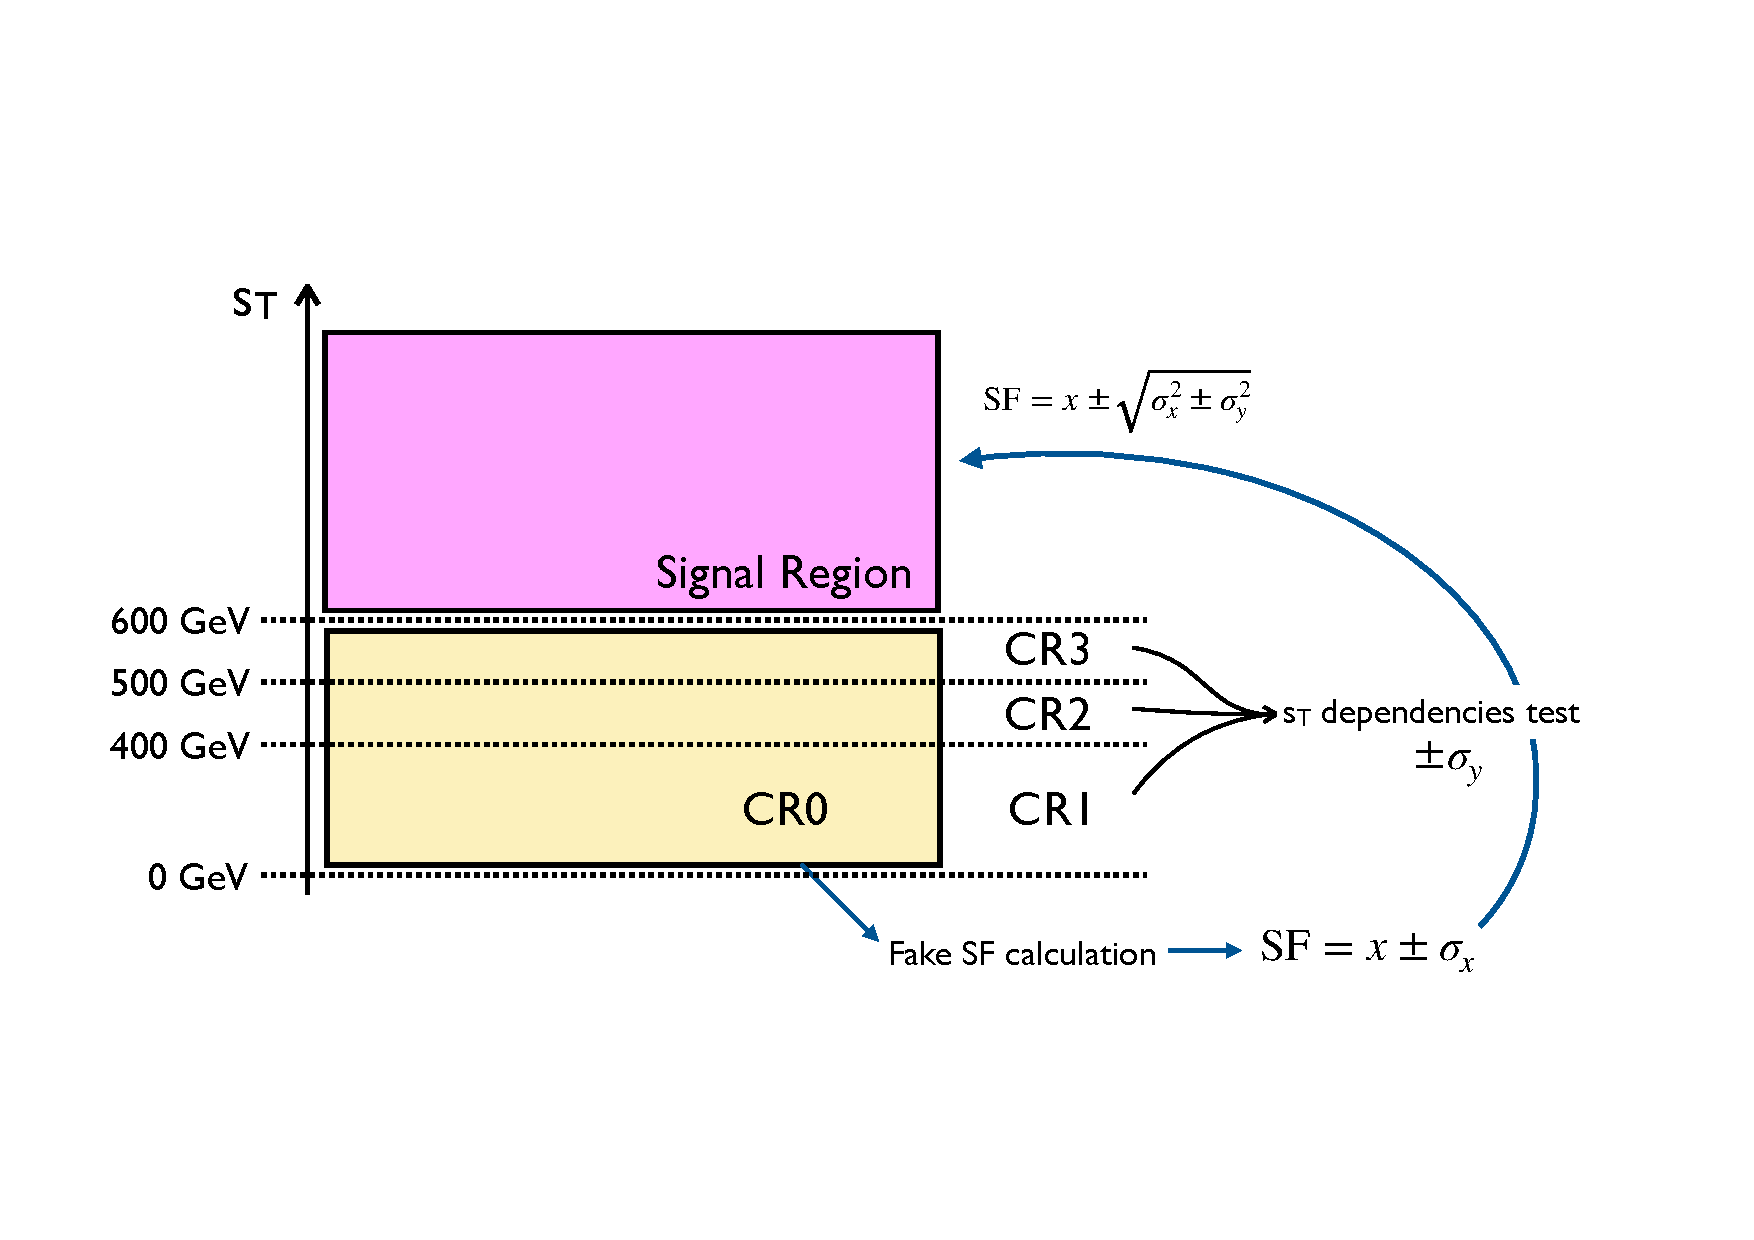
\includegraphics[scale=0.35]{overview_control_region}
  \end{figure}

  \begin{itemize}
    \item There are two types of CR
      \begin{itemize}
        \item CR0 : \\ 
          The actual SFs are derived from the region.
        \item CR1, CR2, CR3 : \\
          These regions are the subset of the CR0. The \sT requirements are determined by the available statistics.
          \hyperlink{mtw_vs_st_true}{\beamerbutton{\mtw vs \sT (true \ttbar)}}
          \hyperlink{mtw_vs_st_fake}{\beamerbutton{\mtw vs \sT (fake \ttbar)}}
      \end{itemize}
  \end{itemize}
\end{frame}


%\begin{frame}{\mtw binning}
%  \vspace{5mm}
%  \ttbar \mtw distribution ($\tau p_T > 100$)\\
%  In the higher energy region, there are few entries $\to$ the rough binning is needed.
%  \begin{figure}
%      \hspace{-6mm}
%      \setcounter{subfigure}{0}
%        \subfloat[\ttbar, 1 prong]{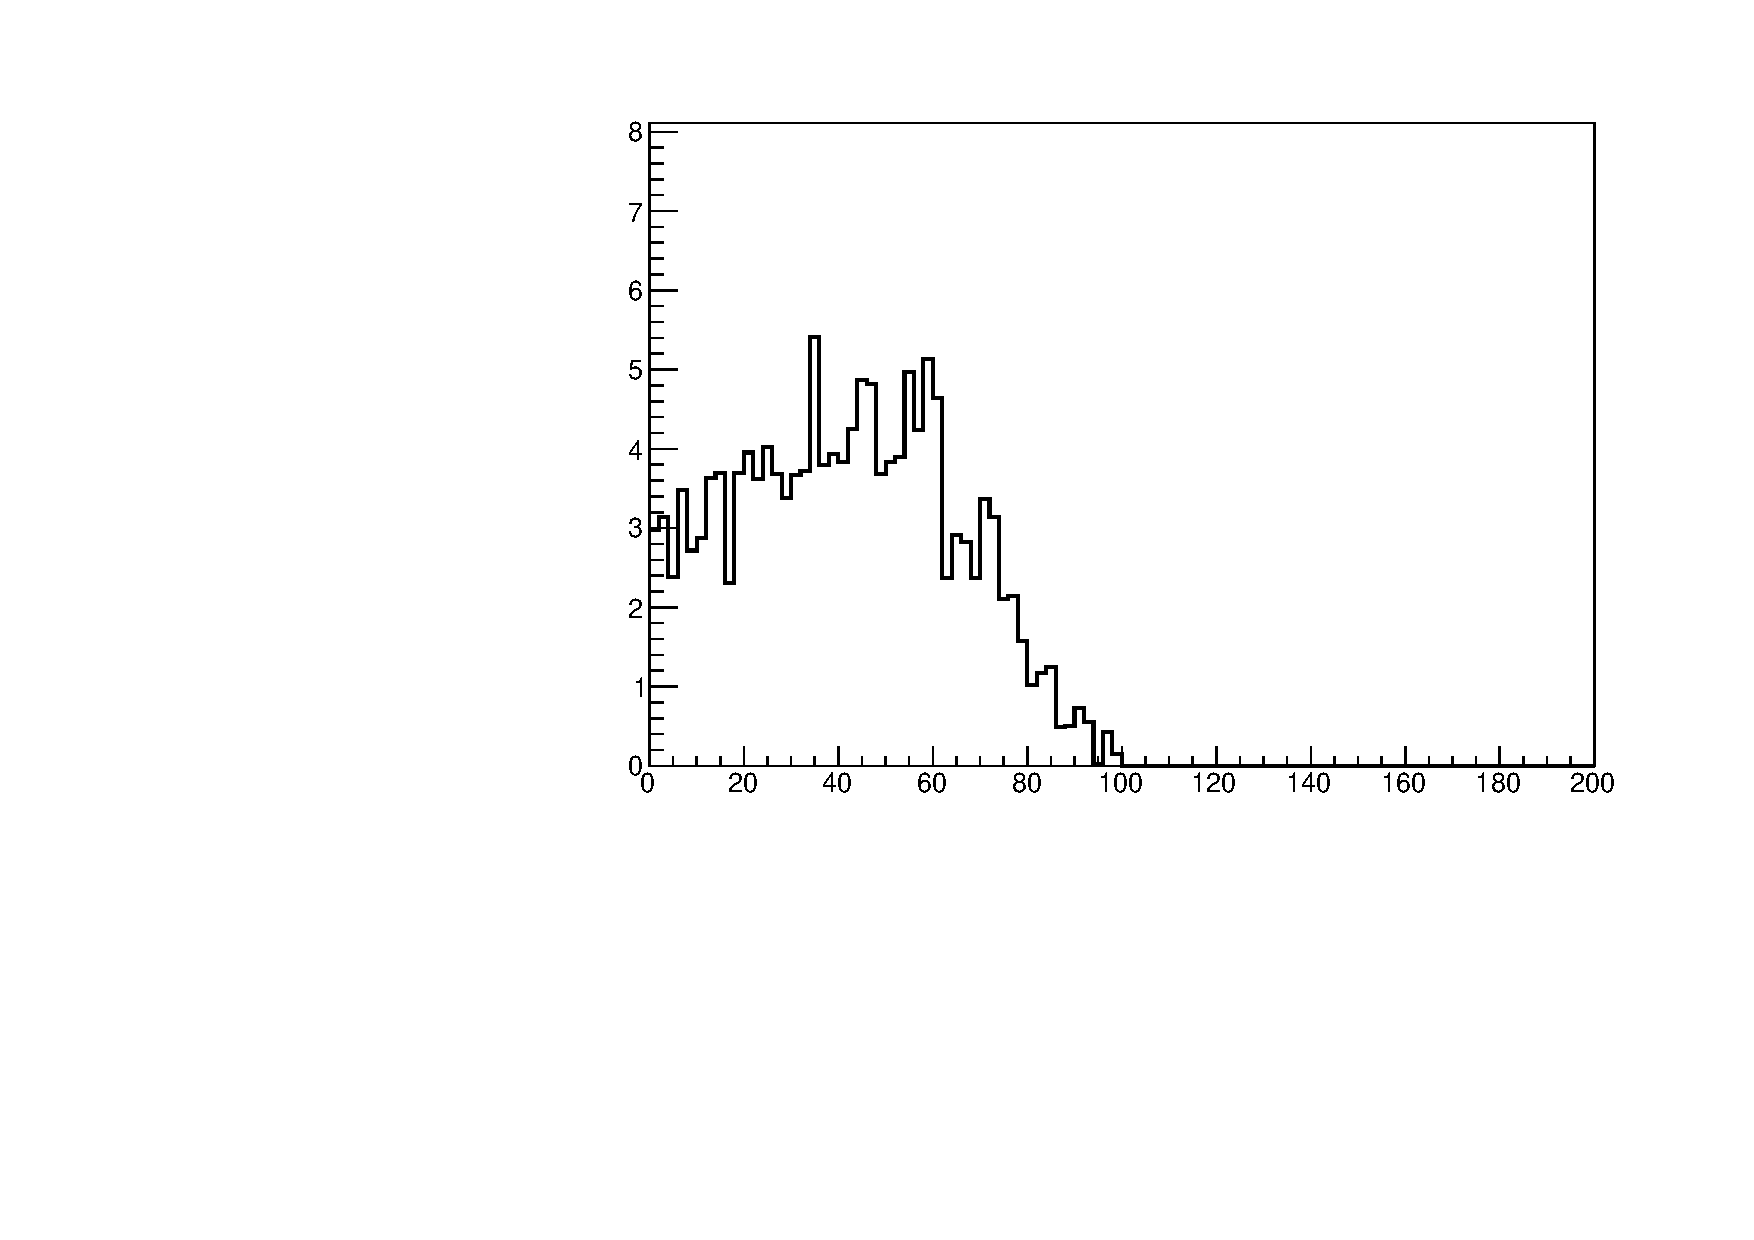
\includegraphics[scale=0.17]{mtw_1P}}
%        \subfloat[\ttbar, 1 prong, rebin]{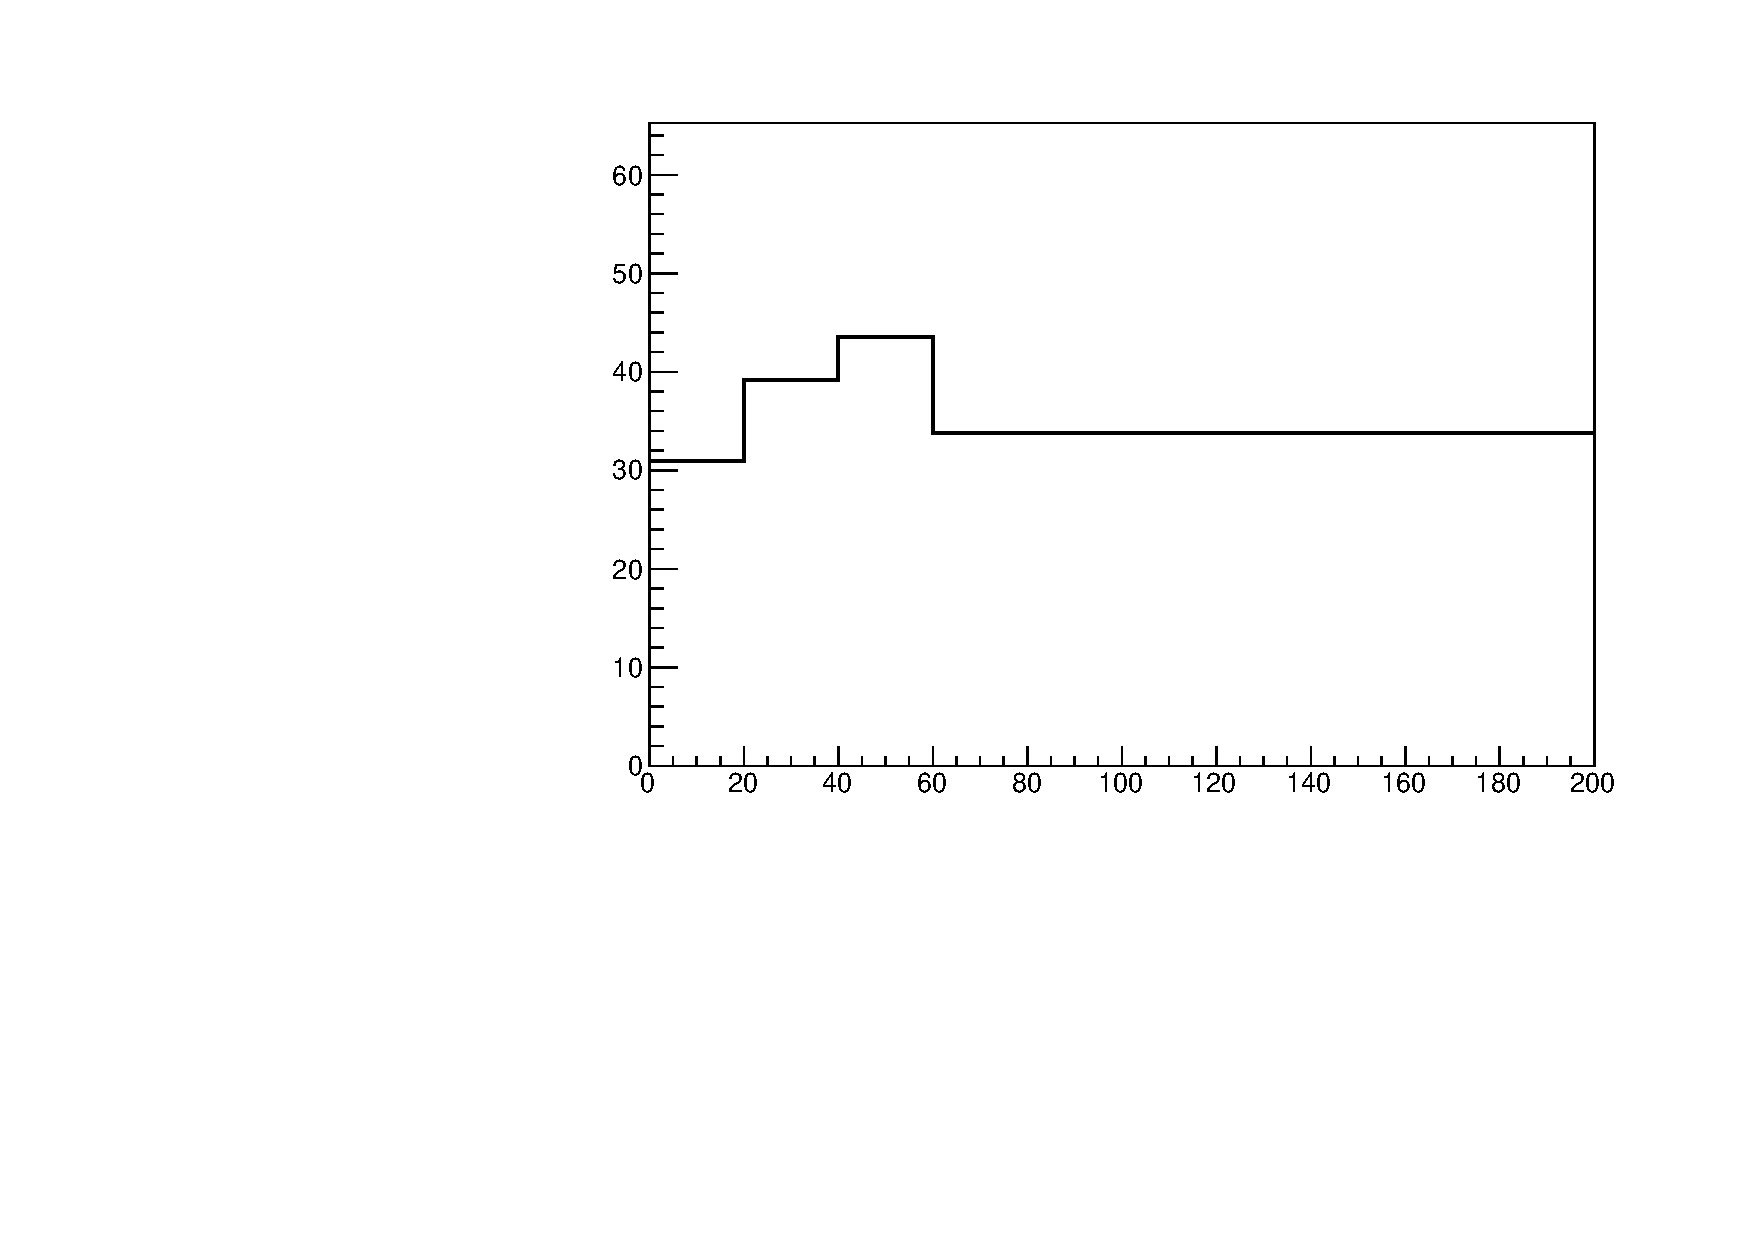
\includegraphics[scale=0.17]{mtw_1P_rebin}}
%        \\
%      \hspace{-6mm}
%      \vspace{10mm}
%        \subfloat[\ttbar, 3 prong]{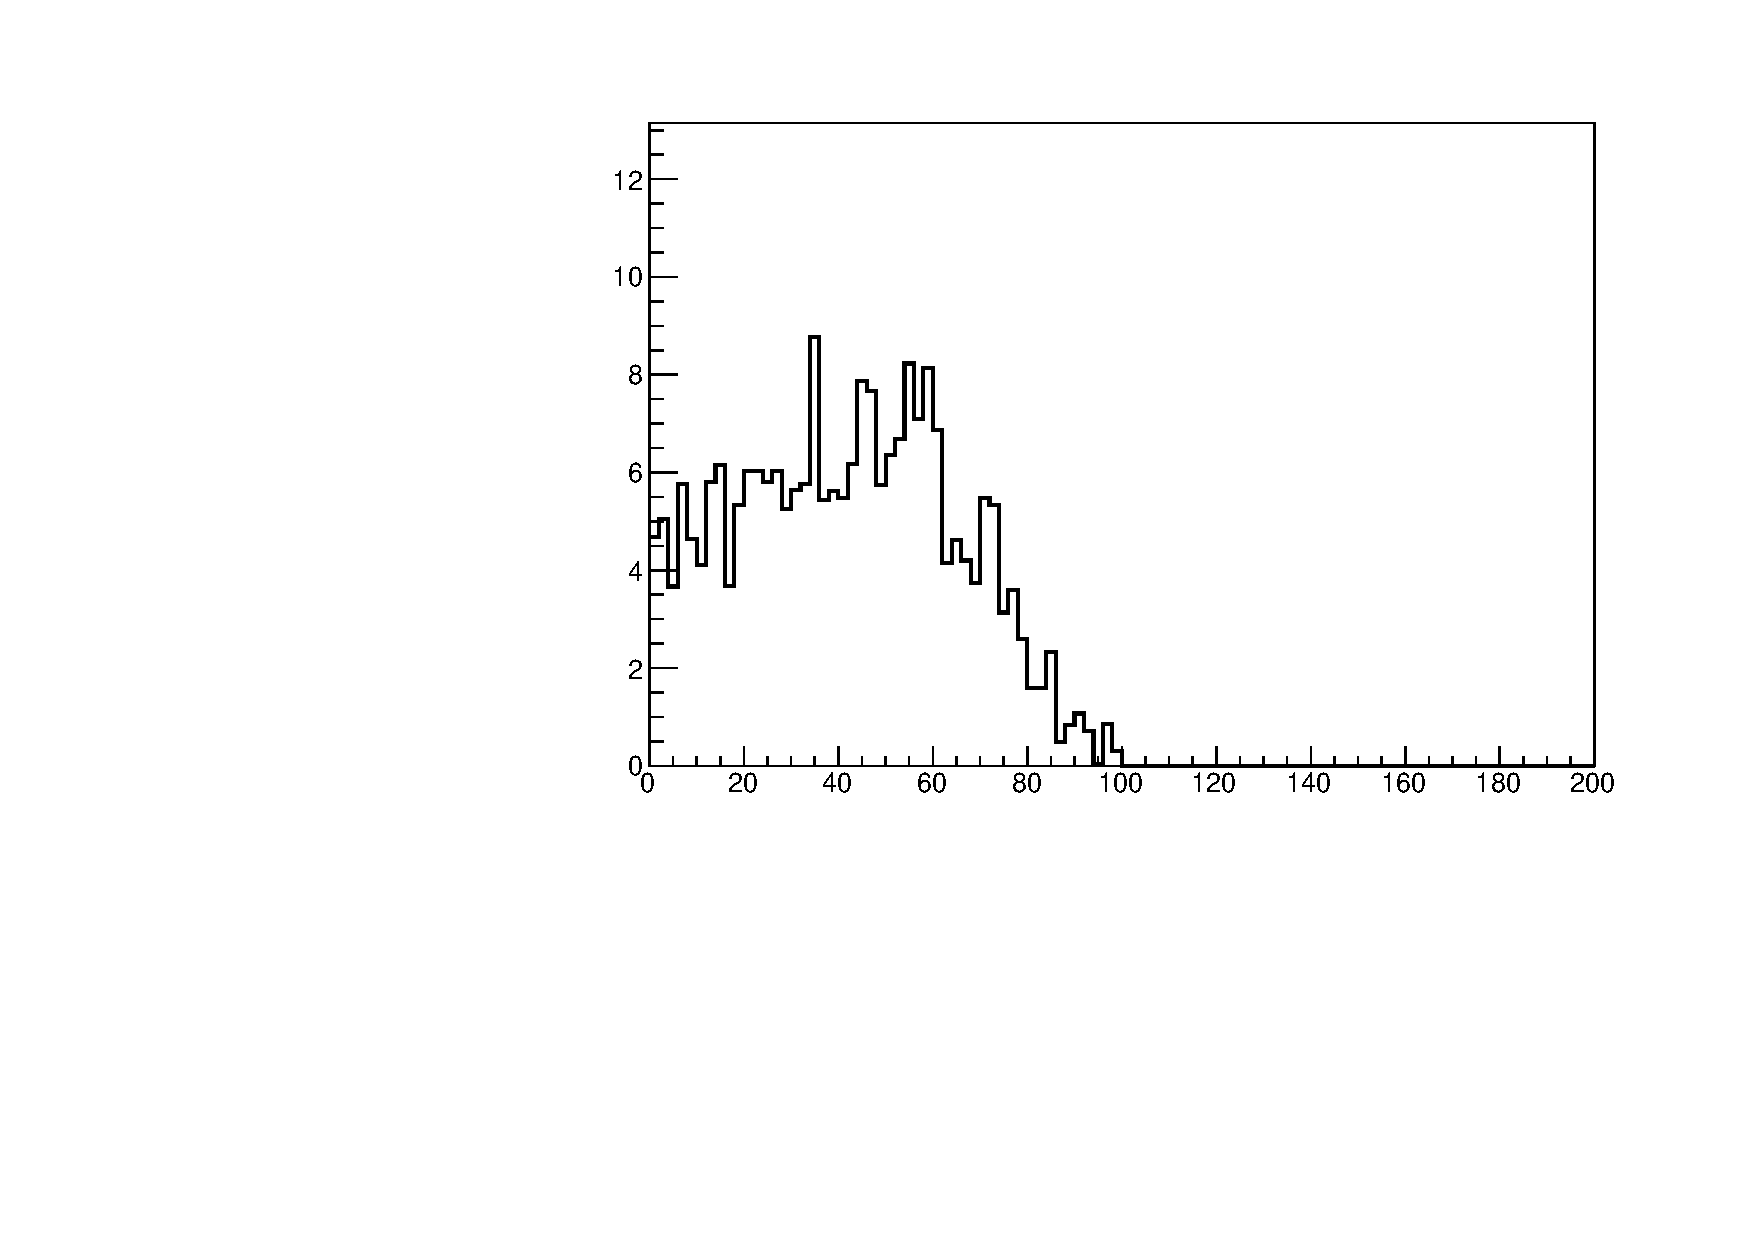
\includegraphics[scale=0.17]{mtw_3P}}
%        \subfloat[\ttbar, 3 prong,rebin]{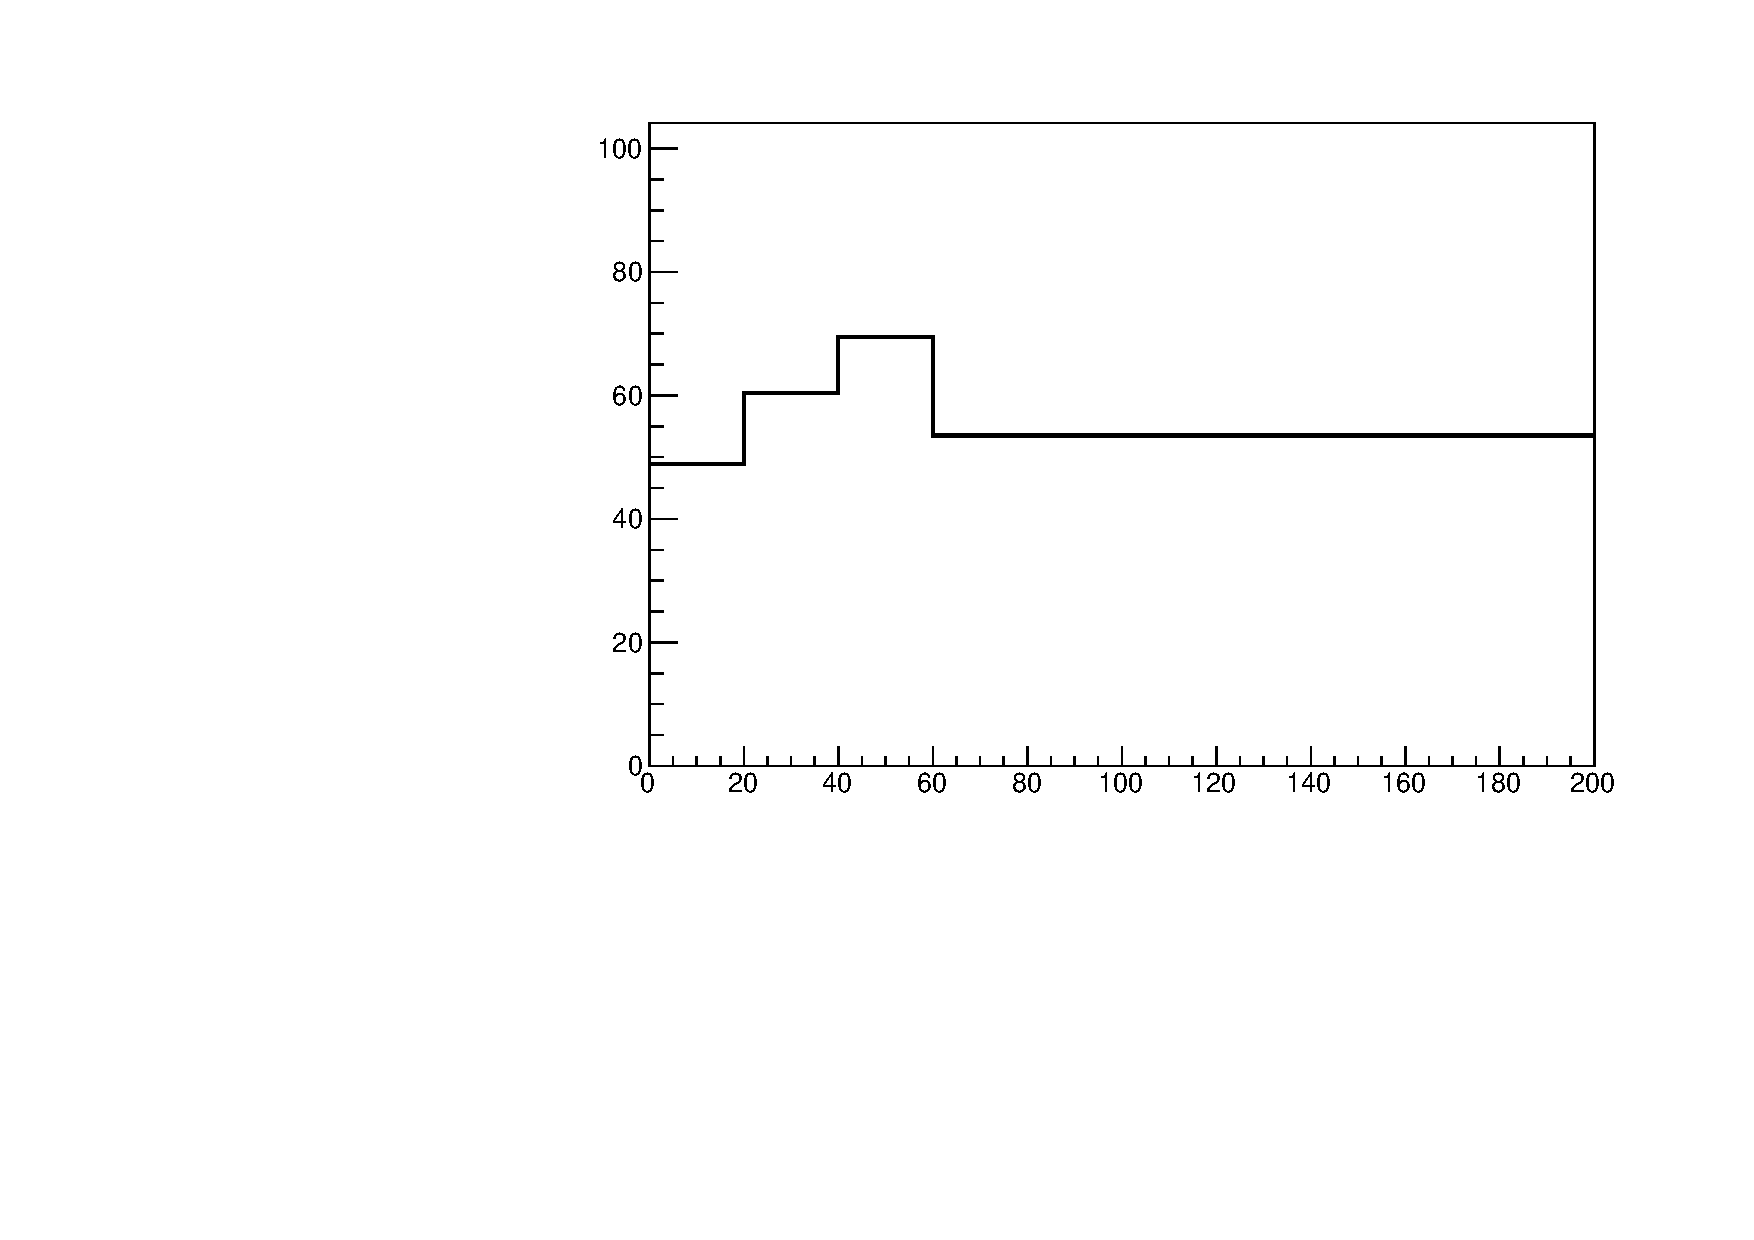
\includegraphics[scale=0.17]{mtw_3P_rebin}}
%  \end{figure}
%\end{frame}

% ====================================================================================== % 
\subtitlepage{\mtw distributions before re-binning}

\begin{frame}{Introduction of \mtw distributions}
  \begin{itemize}
    \item \ttbar fake SF uses the \mtw distributions as the discriminant variables.
    \item It is binned into 4 bins, $[0,40,80,120,\infty]$.
      \begin{itemize}
        \item This binning bounds are determined by the available statistics.
      \end{itemize}
      \vspp 
    \item Higher \mtw bins are pure \ttbar region, while lower bins are admixture.
      \begin{itemize}
        \item So the \mtw distributions are also usefule for the LQ.
      \end{itemize}
  \end{itemize}
\end{frame}

\begin{frame}{\mtw distribution (1-prong, CR1)}
  \begin{figure}
    \setcounter{subfigure}{0}
    \centering
        \subfloat[$p_T<35$]    {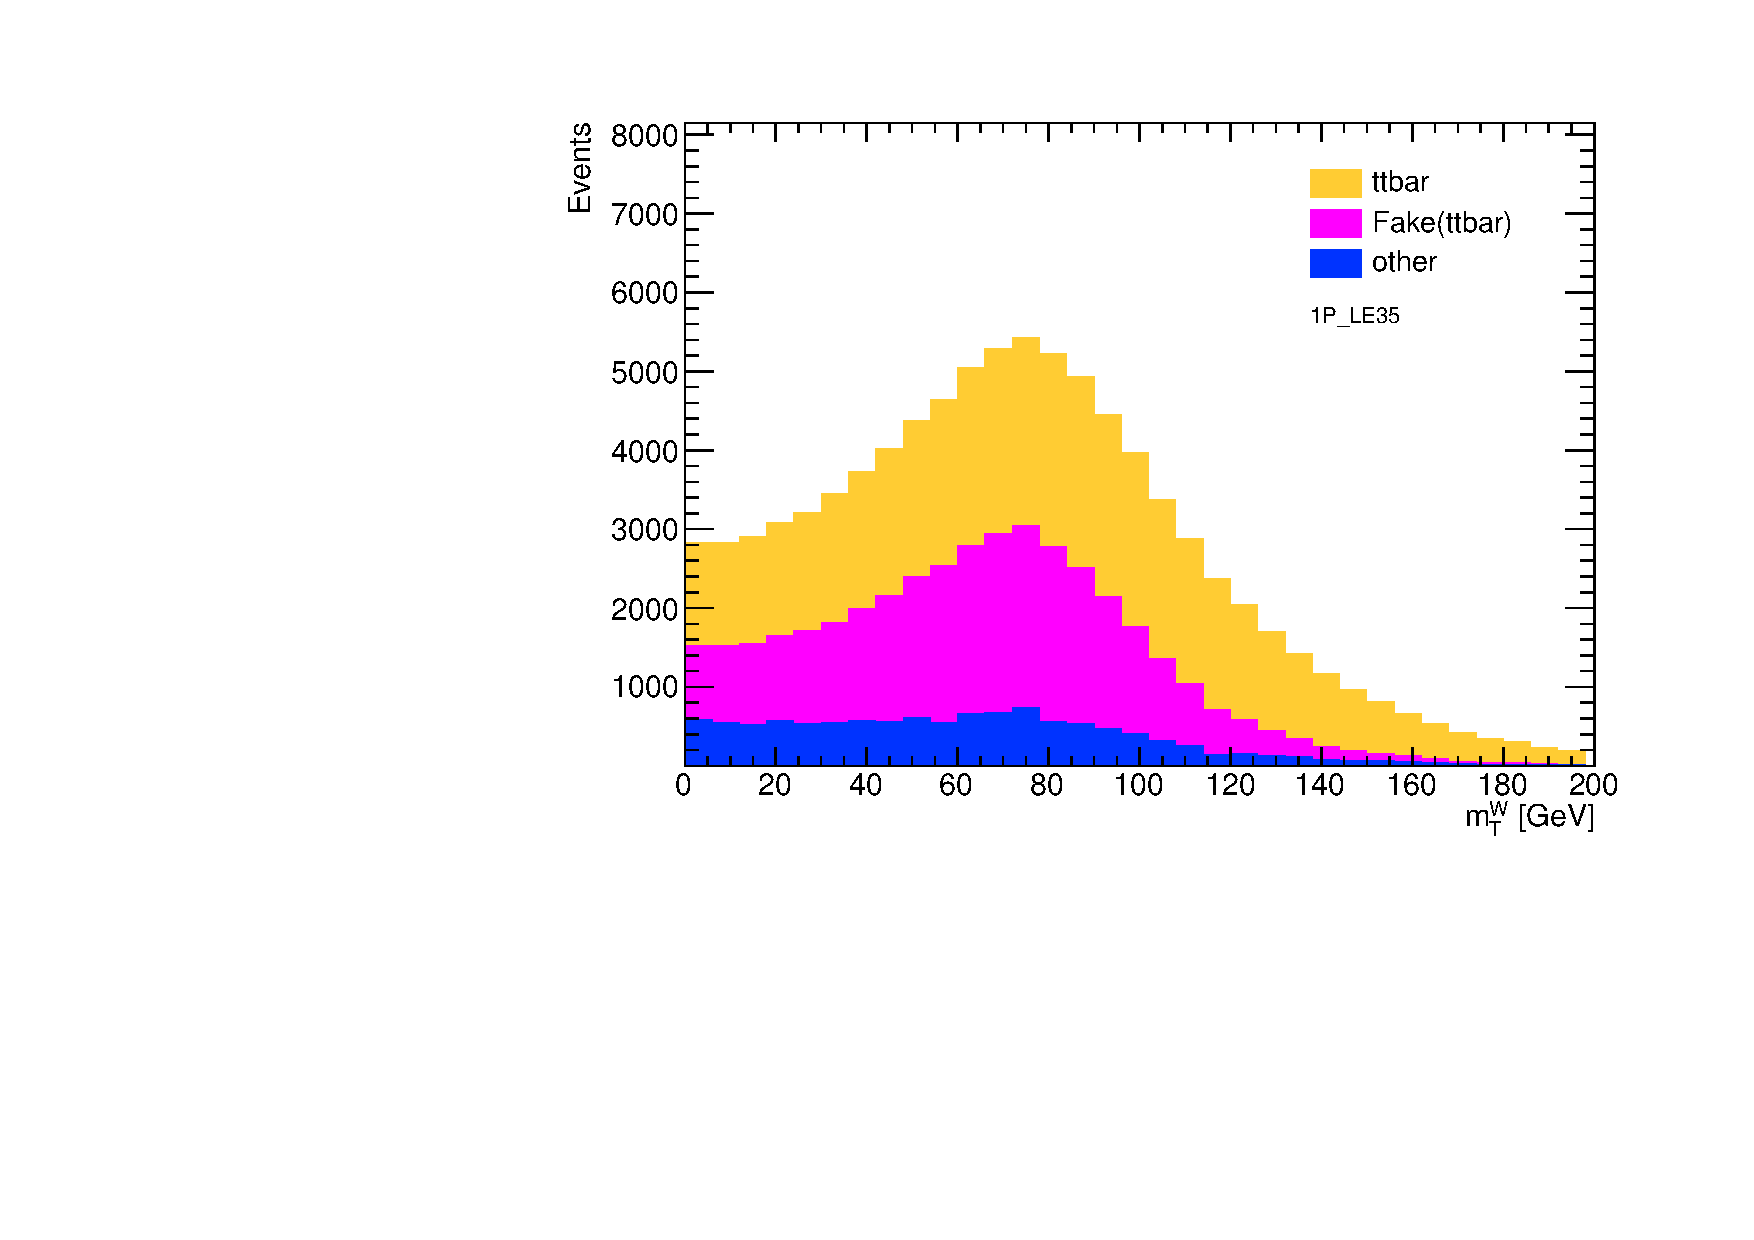
\includegraphics[scale=0.15]{mtw_fine_binning_stLT400_1P_LE35}}
        \subfloat[$35<p_T<40$] {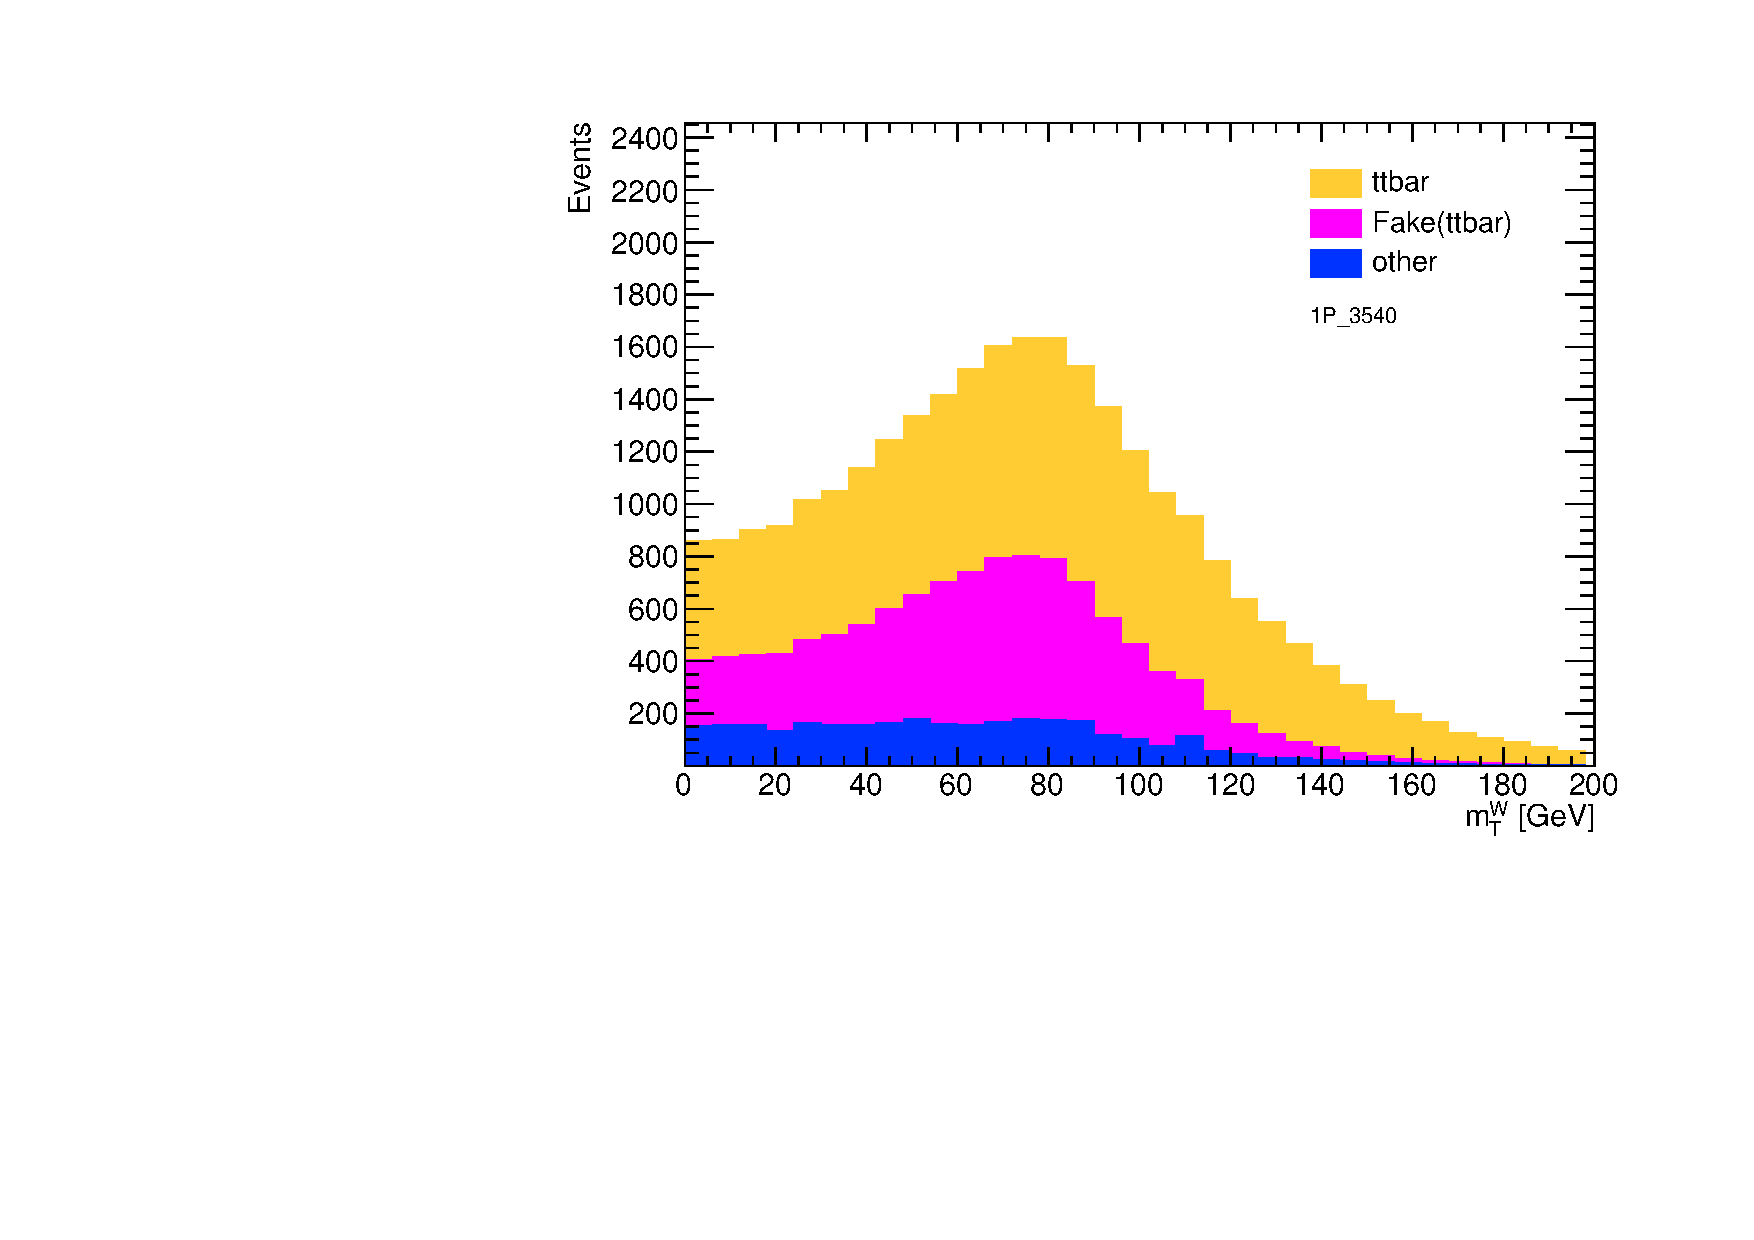
\includegraphics[scale=0.15]{mtw_fine_binning_stLT400_1P_3540}}
        \subfloat[$40<p_T<45$] {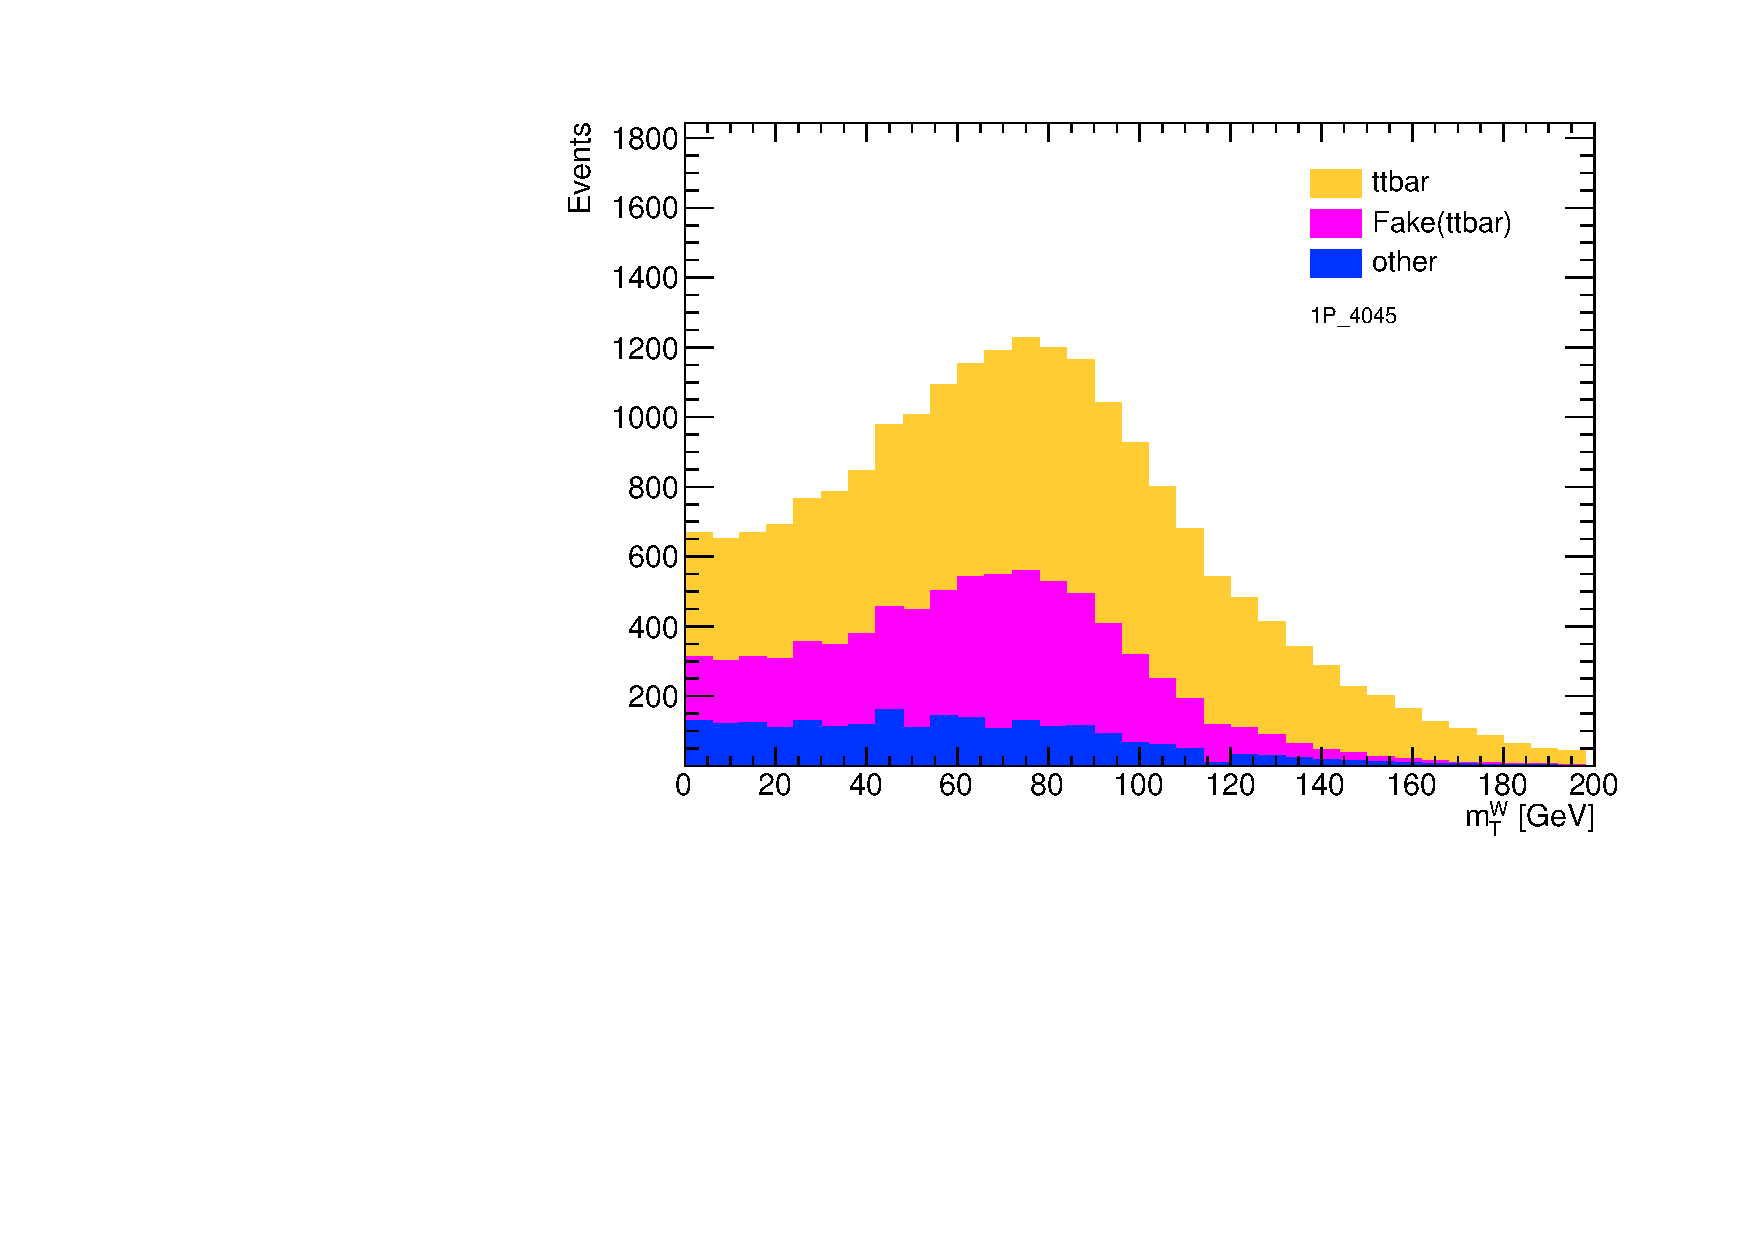
\includegraphics[scale=0.15]{mtw_fine_binning_stLT400_1P_4045}}
        \subfloat[$45<p_T<50$] {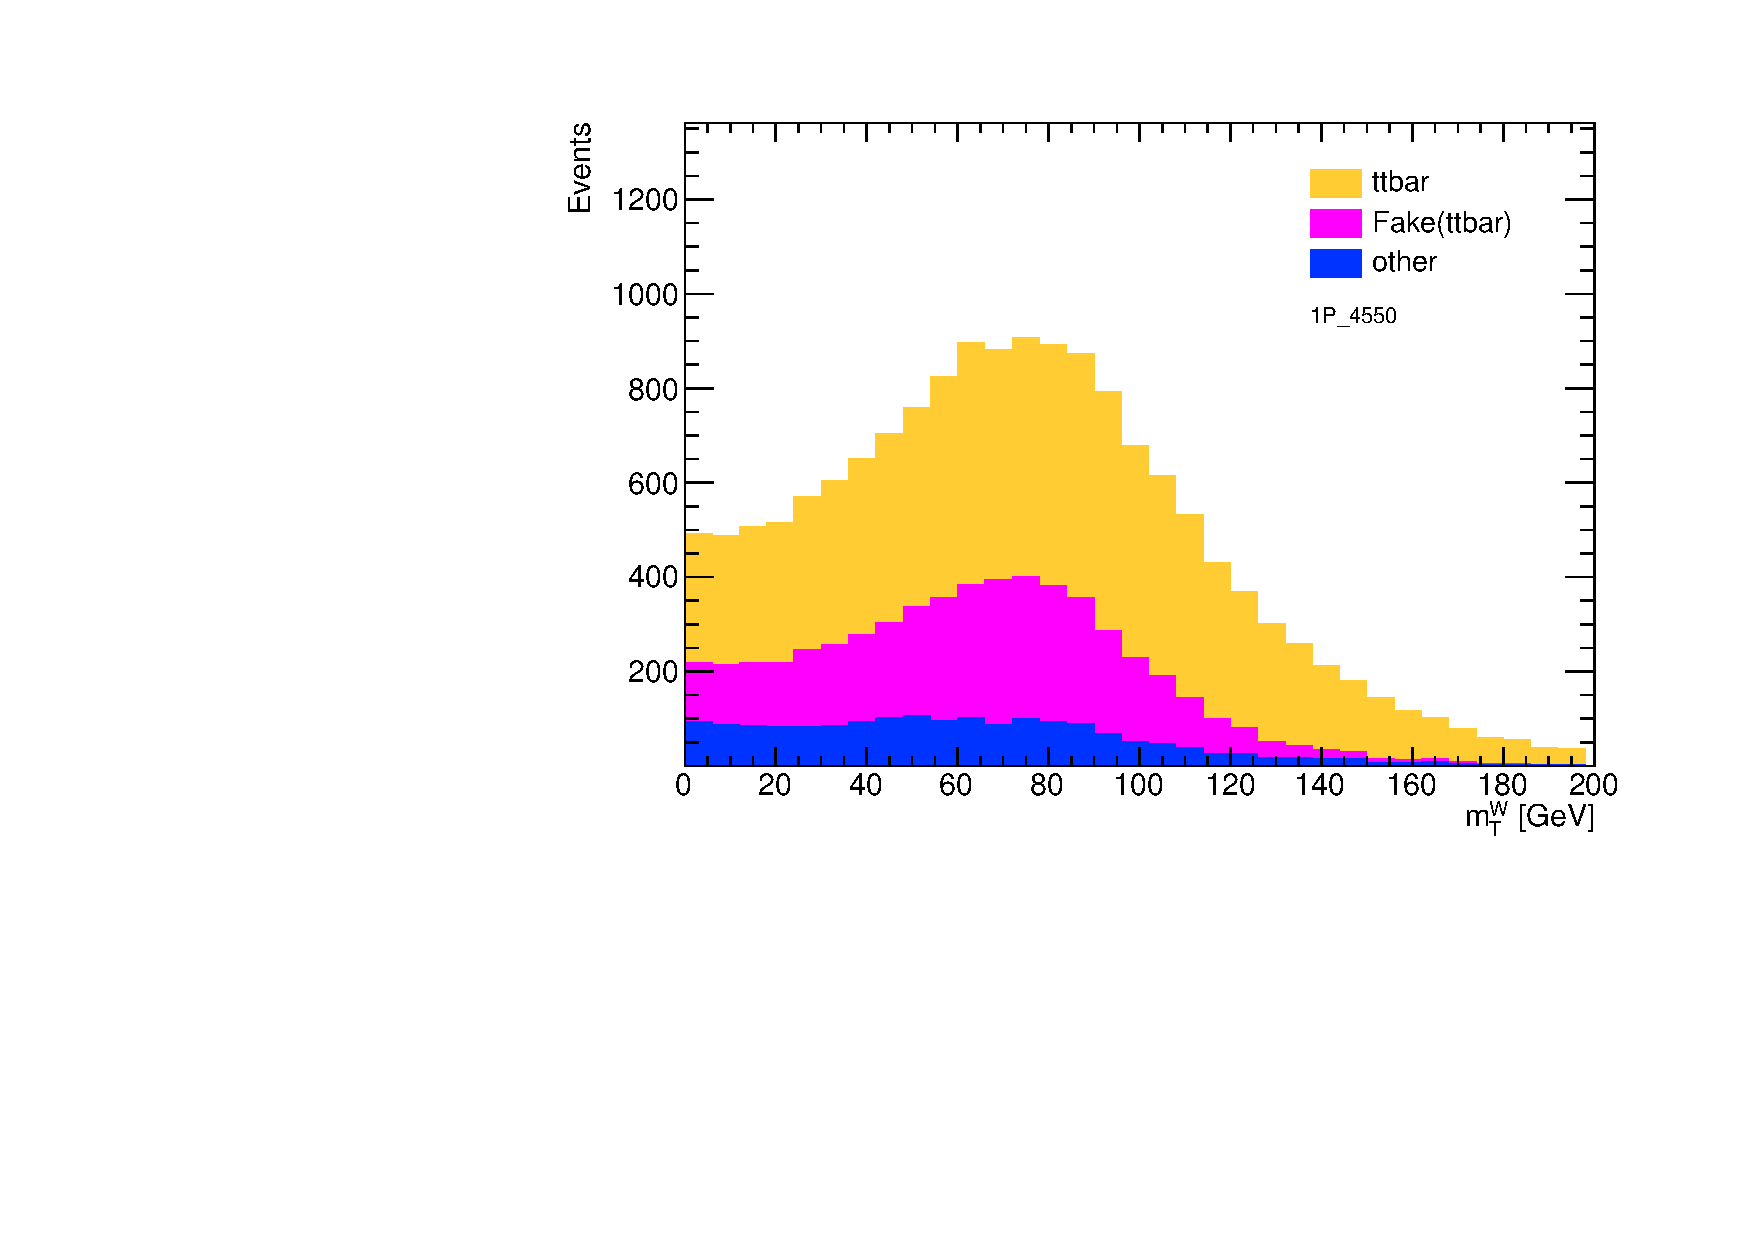
\includegraphics[scale=0.15]{mtw_fine_binning_stLT400_1P_4550}} \\
        \subfloat[$50<p_T<55$] {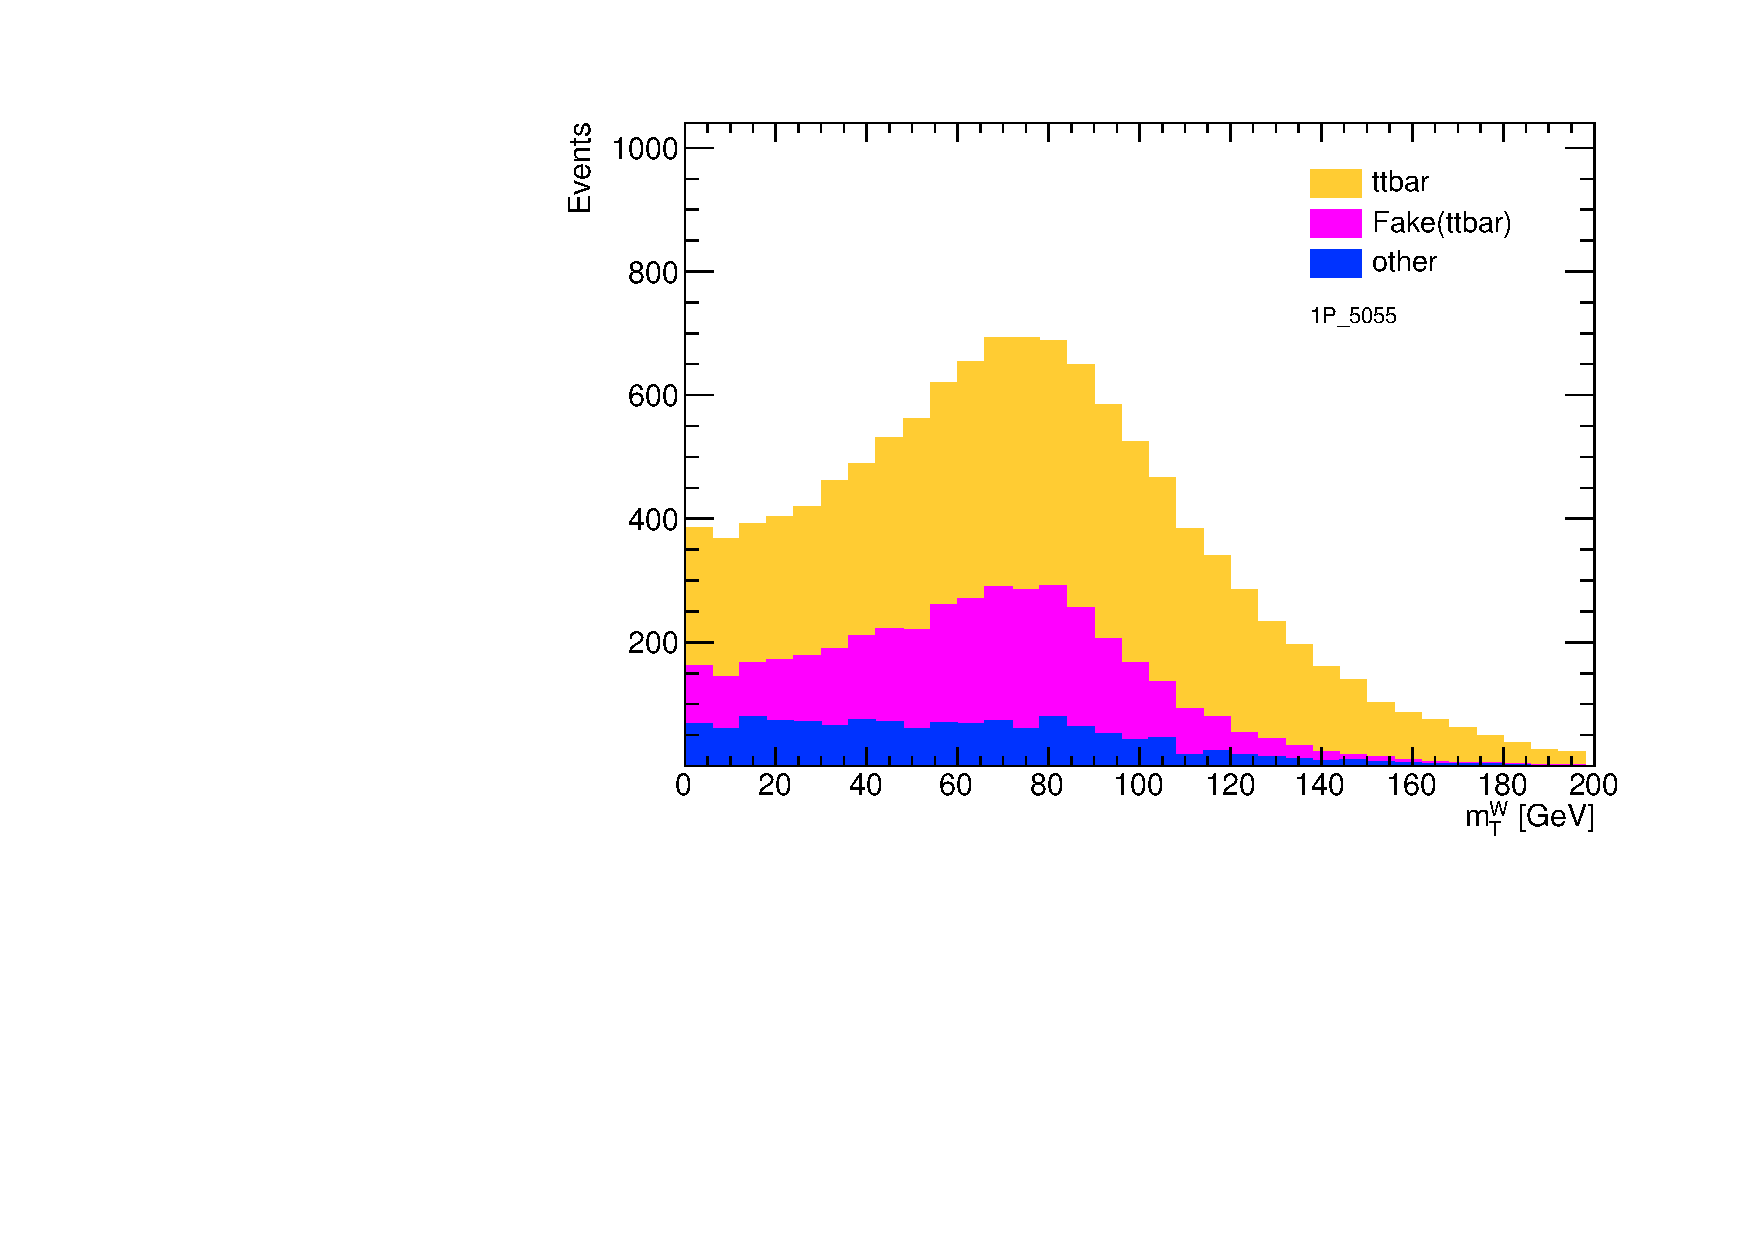
\includegraphics[scale=0.15]{mtw_fine_binning_stLT400_1P_5055}}
        \subfloat[$55<p_T<70$] {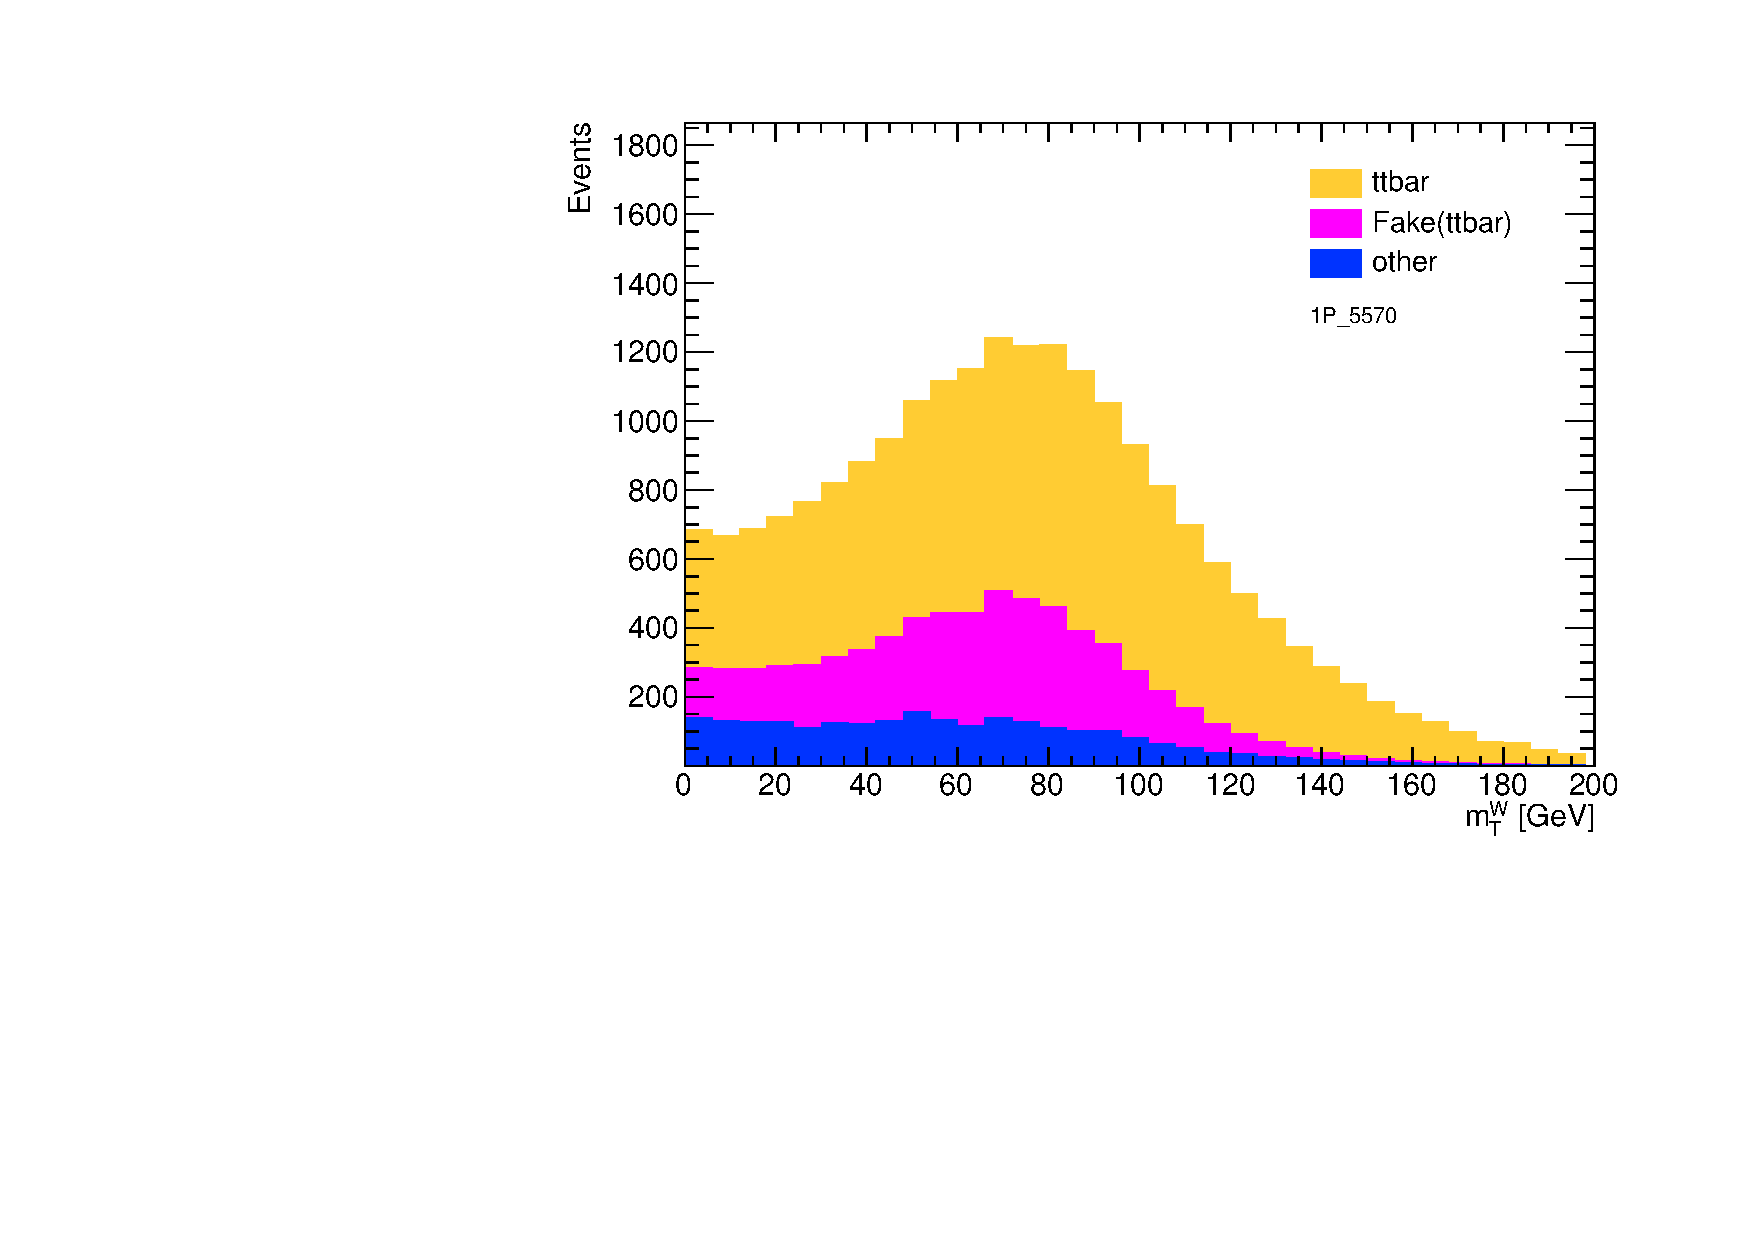
\includegraphics[scale=0.15]{mtw_fine_binning_stLT400_1P_5570}}
        \subfloat[$70<p_T<100$]{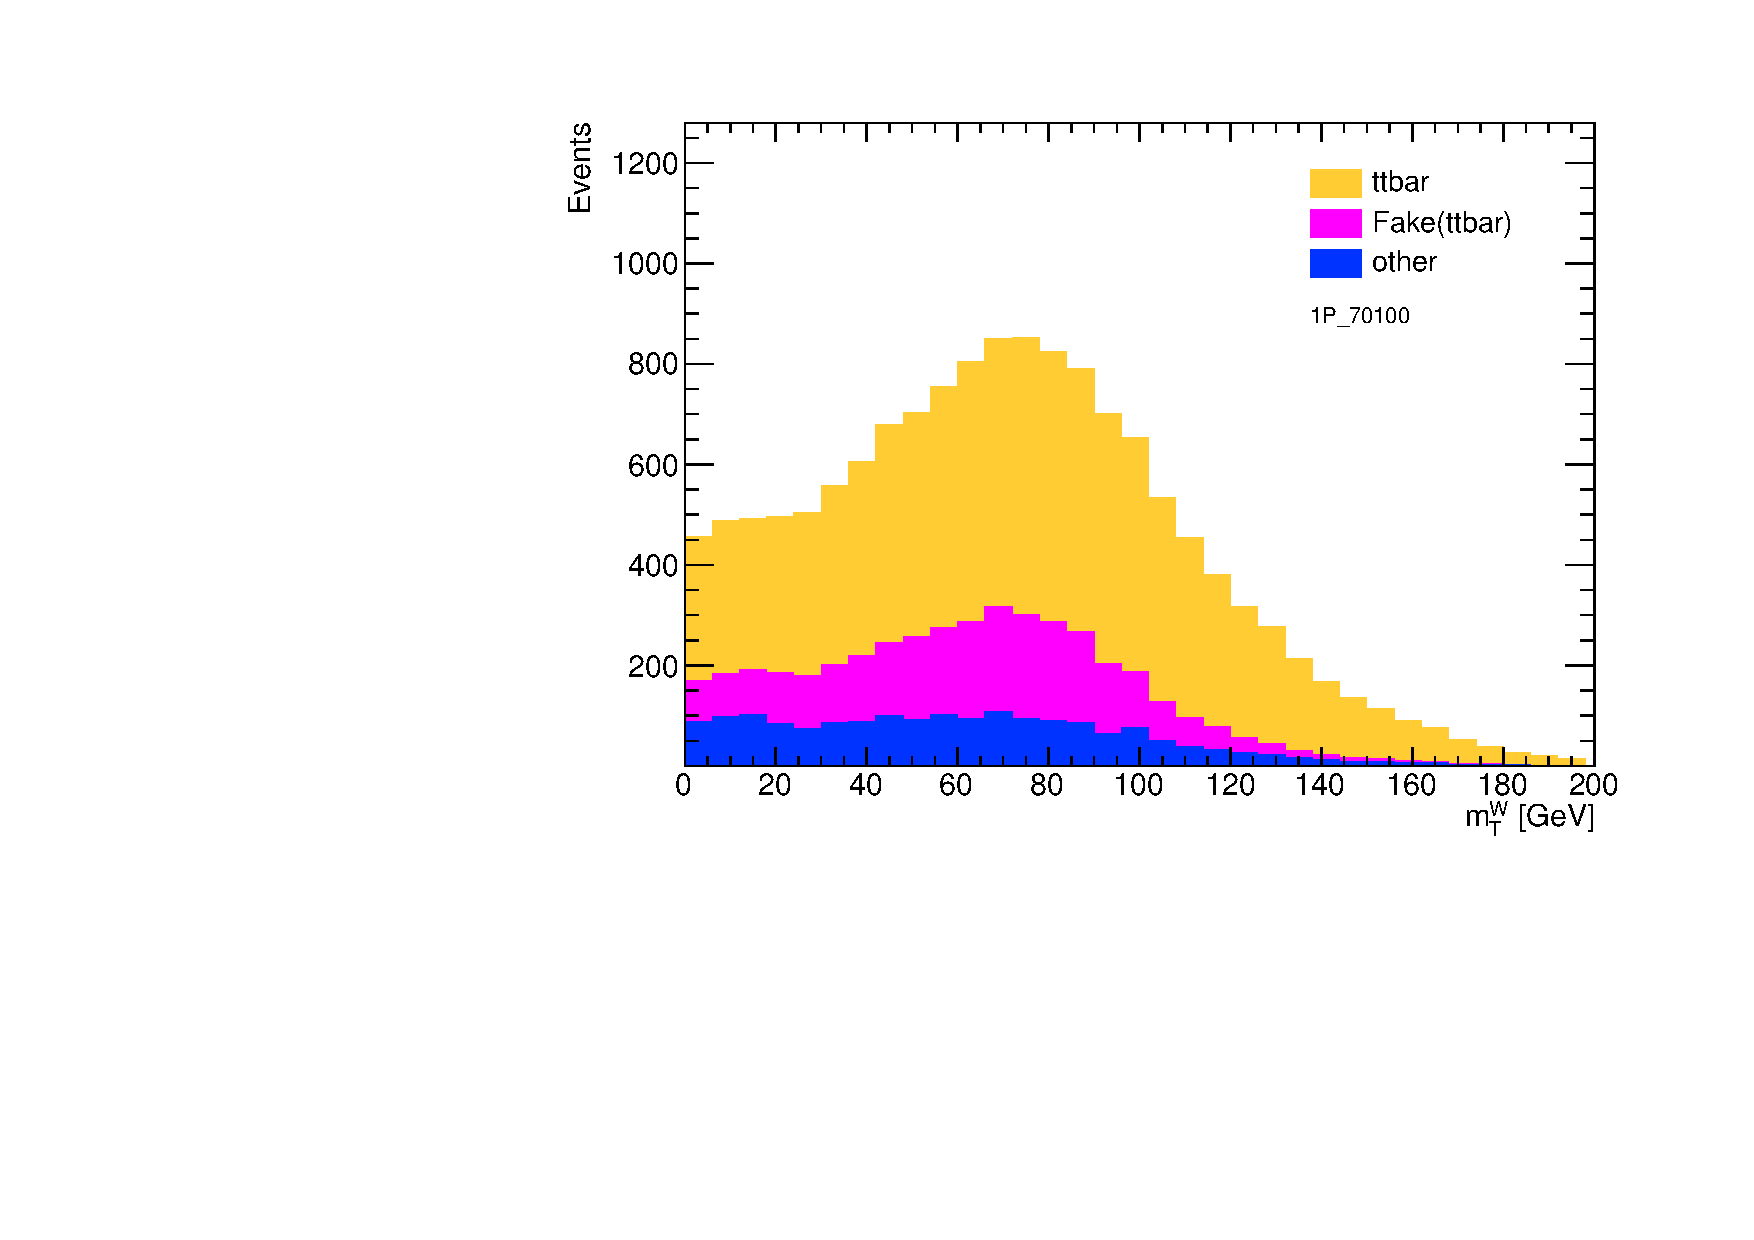
\includegraphics[scale=0.15]{mtw_fine_binning_stLT400_1P_70100}}
        \subfloat[$100<p_T$]   {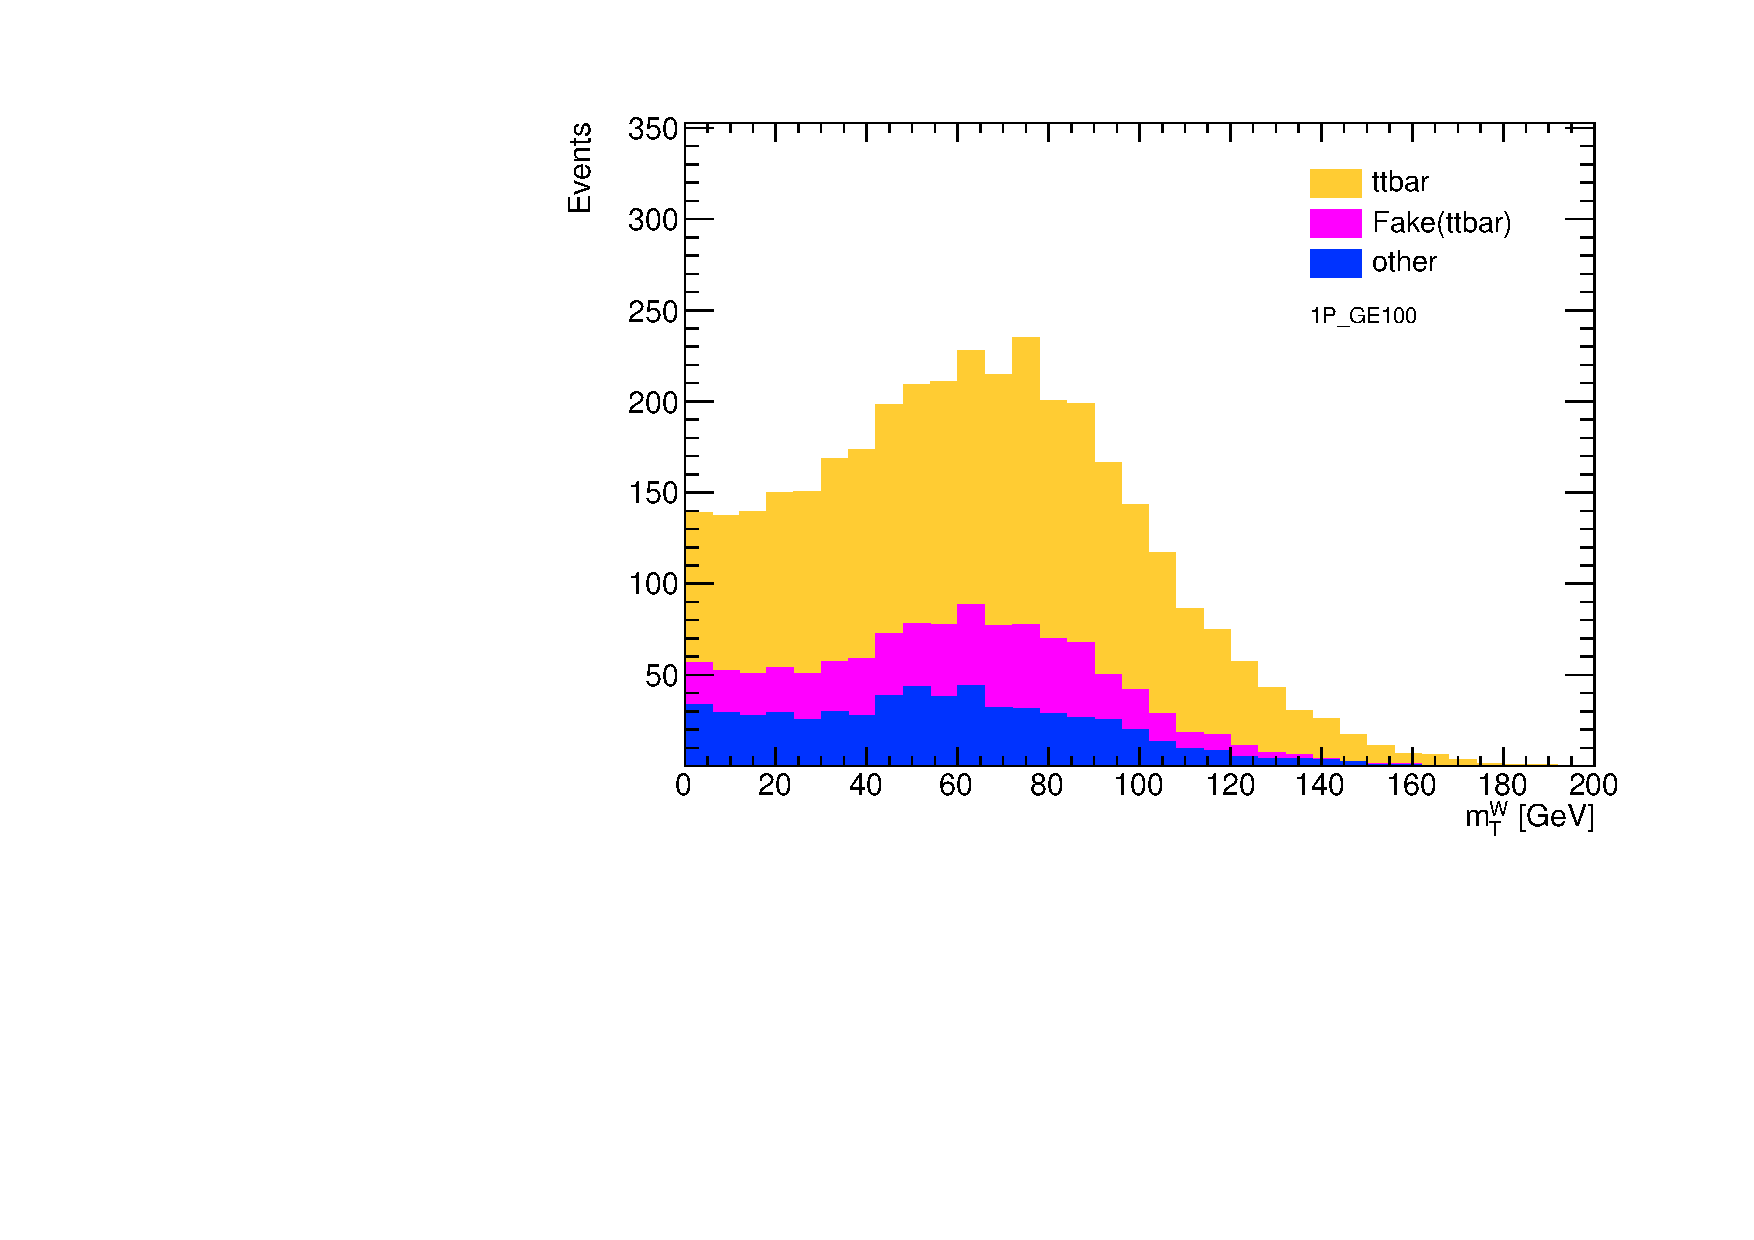
\includegraphics[scale=0.15]{mtw_fine_binning_stLT400_1P_GE100}}\\
  \end{figure}
\end{frame}

\begin{frame}{\mtw distribution (3-prong, CR1)}
  \begin{figure}
    \setcounter{subfigure}{0}
    \centering
        \subfloat[$p_T<35$]    {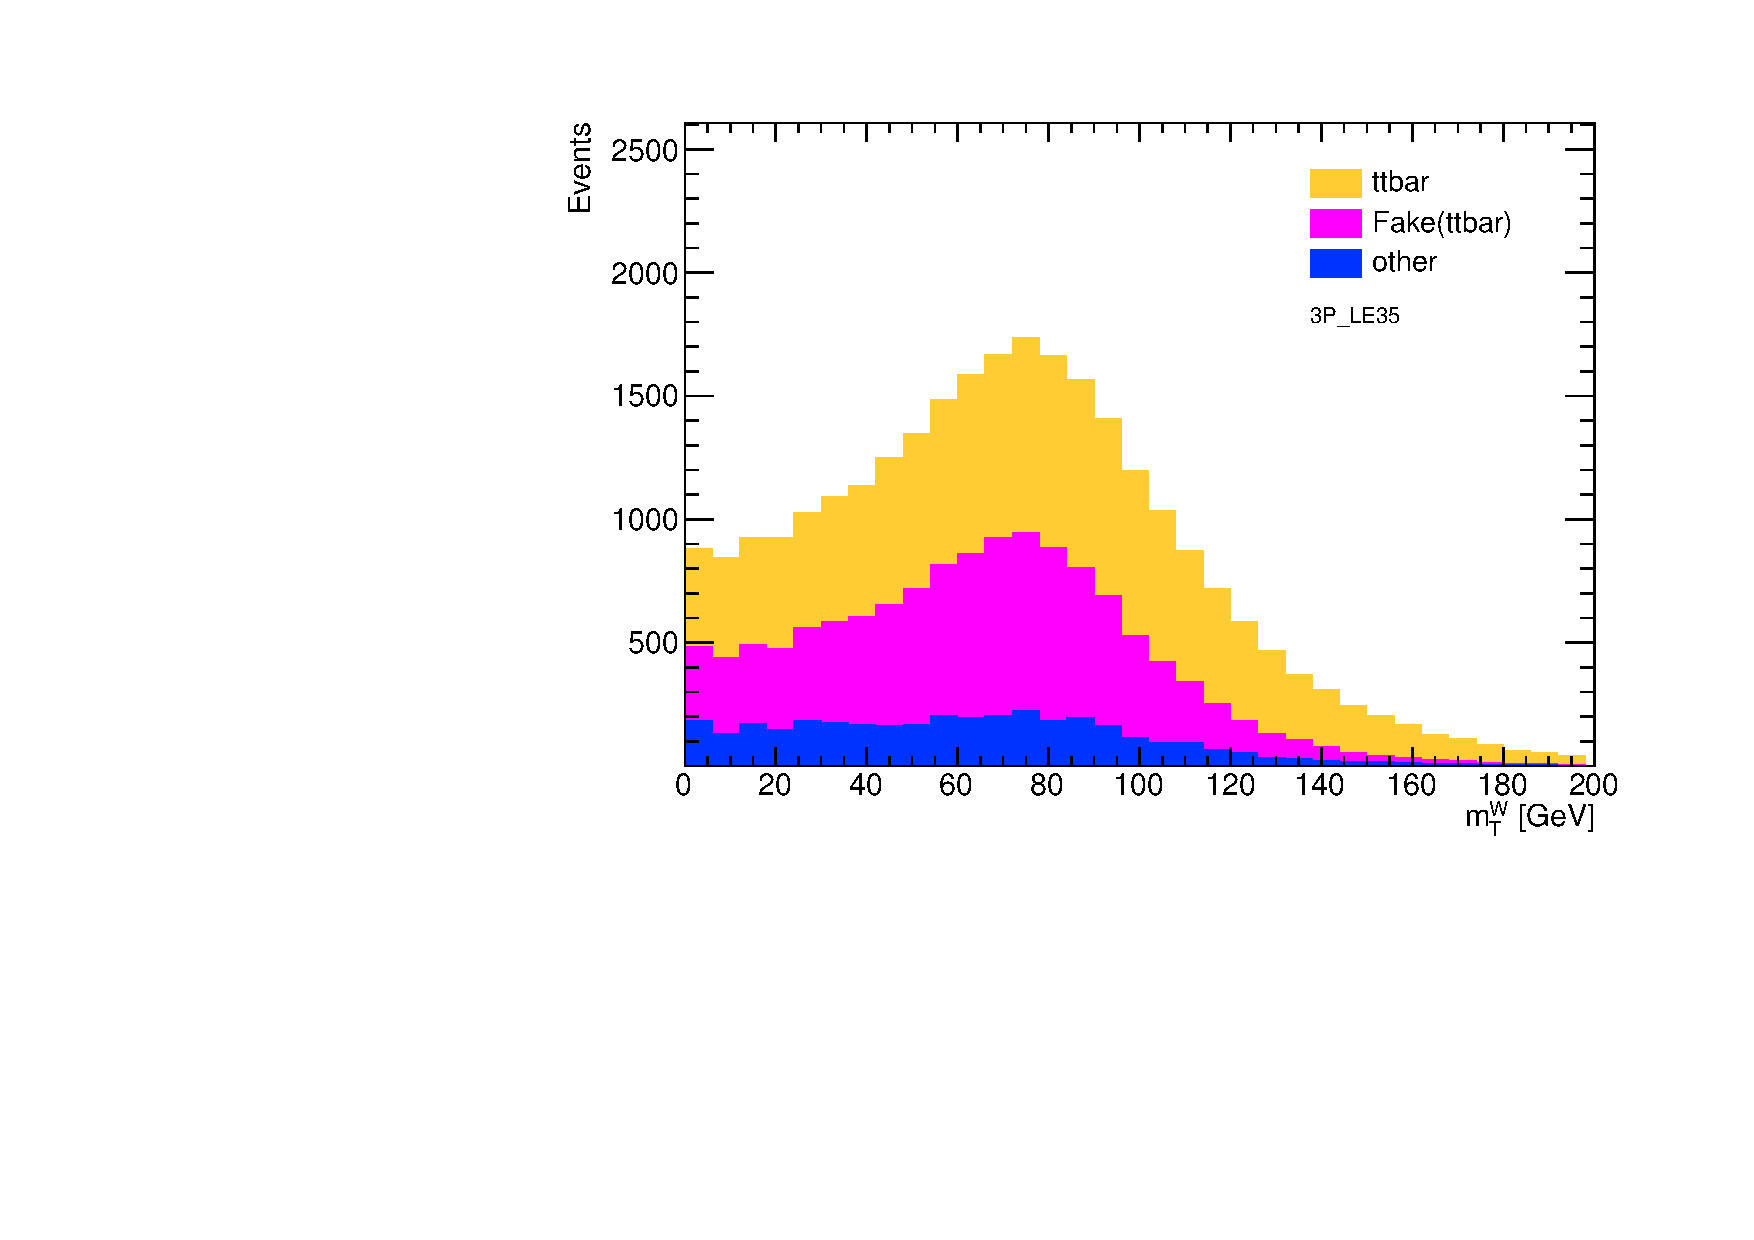
\includegraphics[scale=0.15]{mtw_fine_binning_stLT400_3P_LE35}}
        \subfloat[$35<p_T<40$] {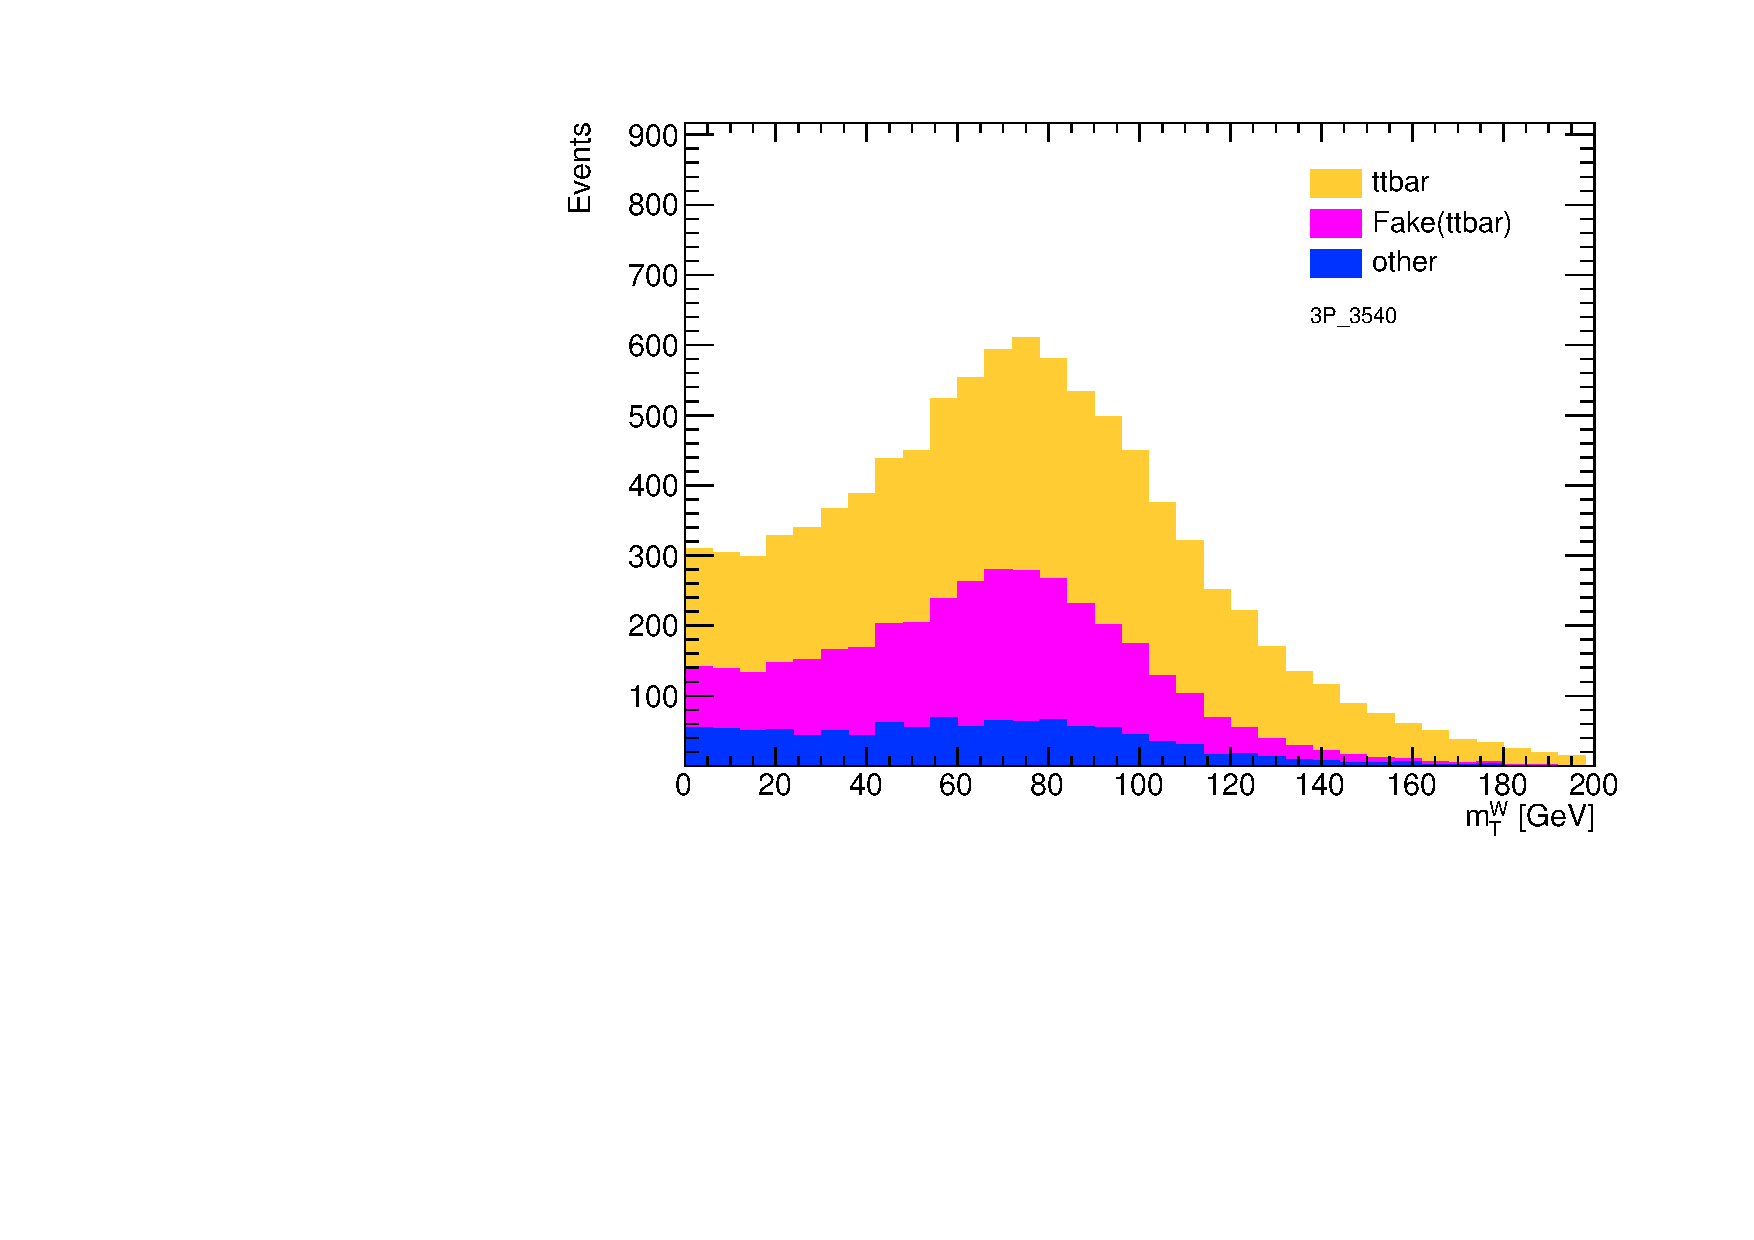
\includegraphics[scale=0.15]{mtw_fine_binning_stLT400_3P_3540}}
        \subfloat[$40<p_T<45$] {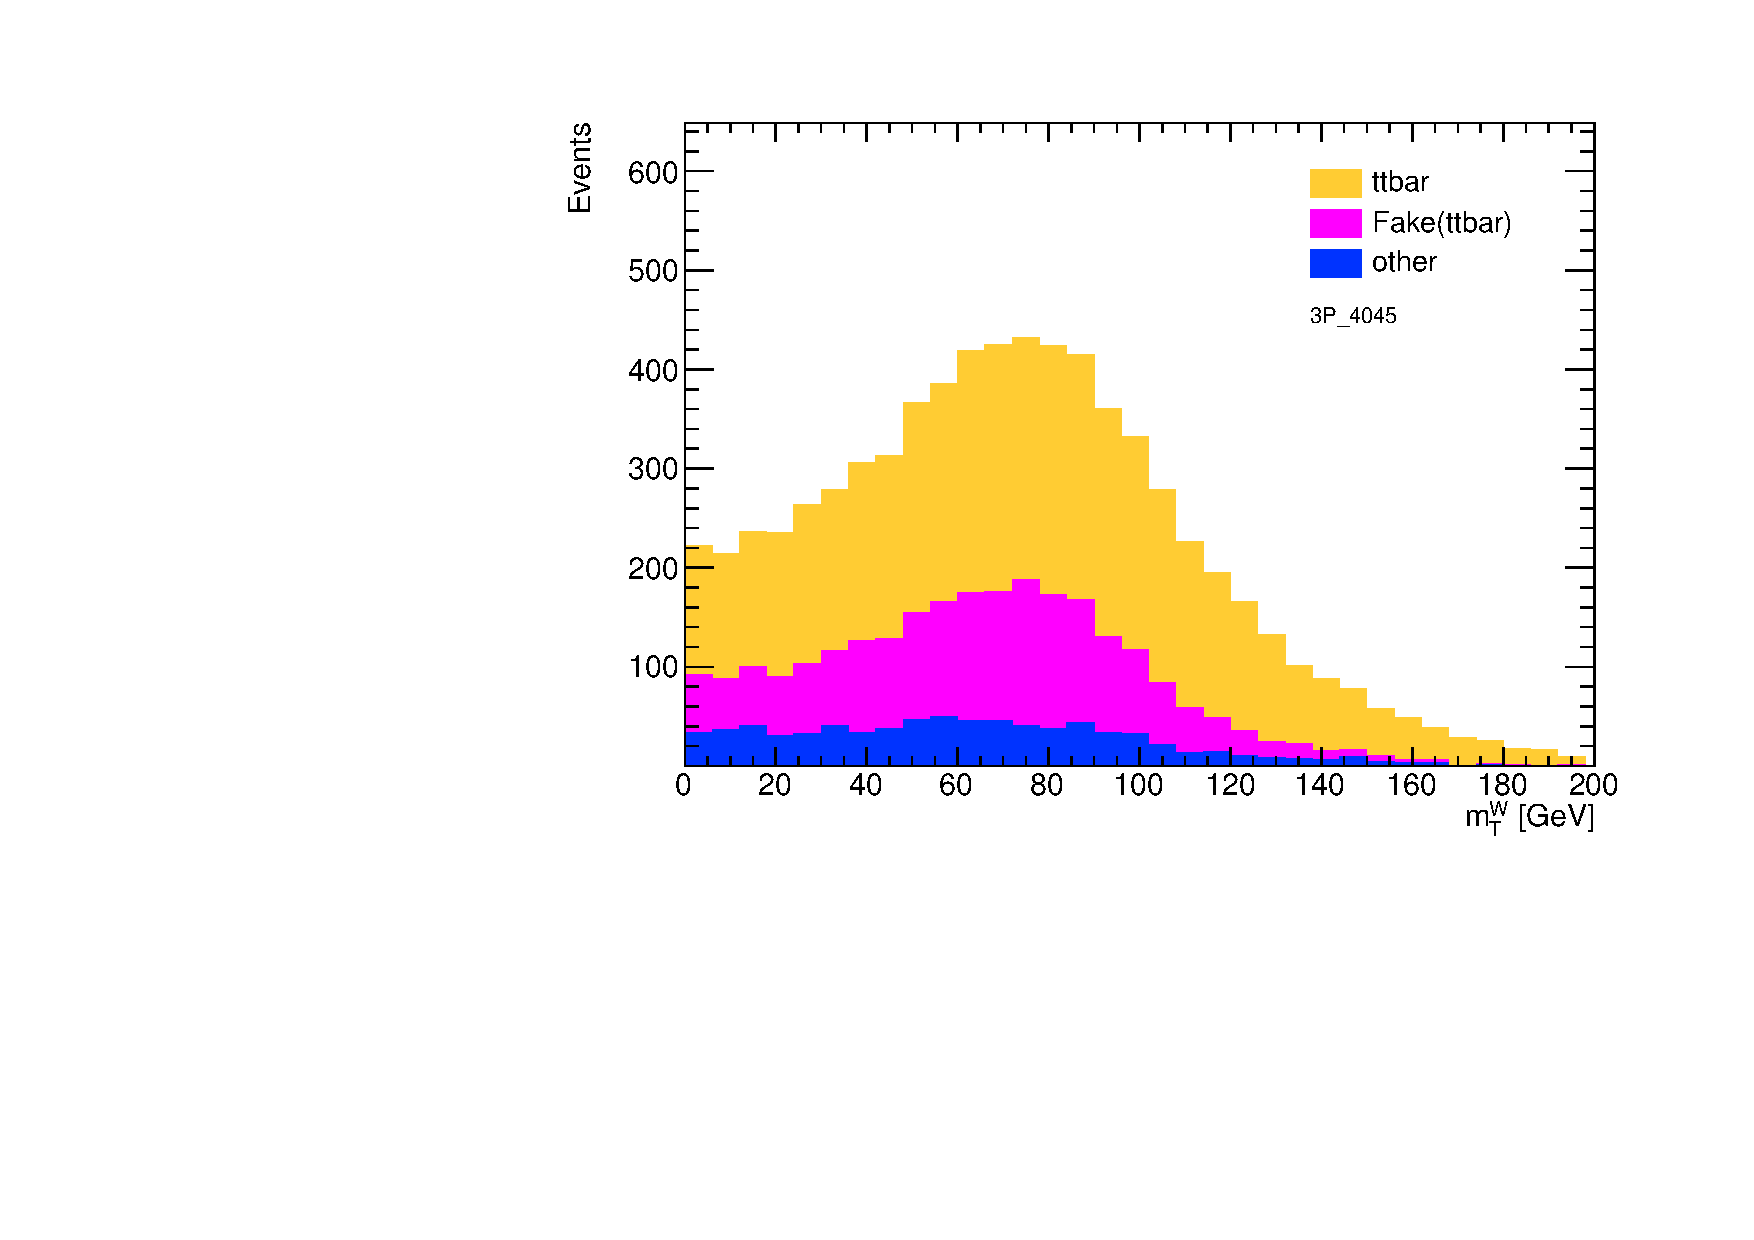
\includegraphics[scale=0.15]{mtw_fine_binning_stLT400_3P_4045}}
        \subfloat[$45<p_T<50$] {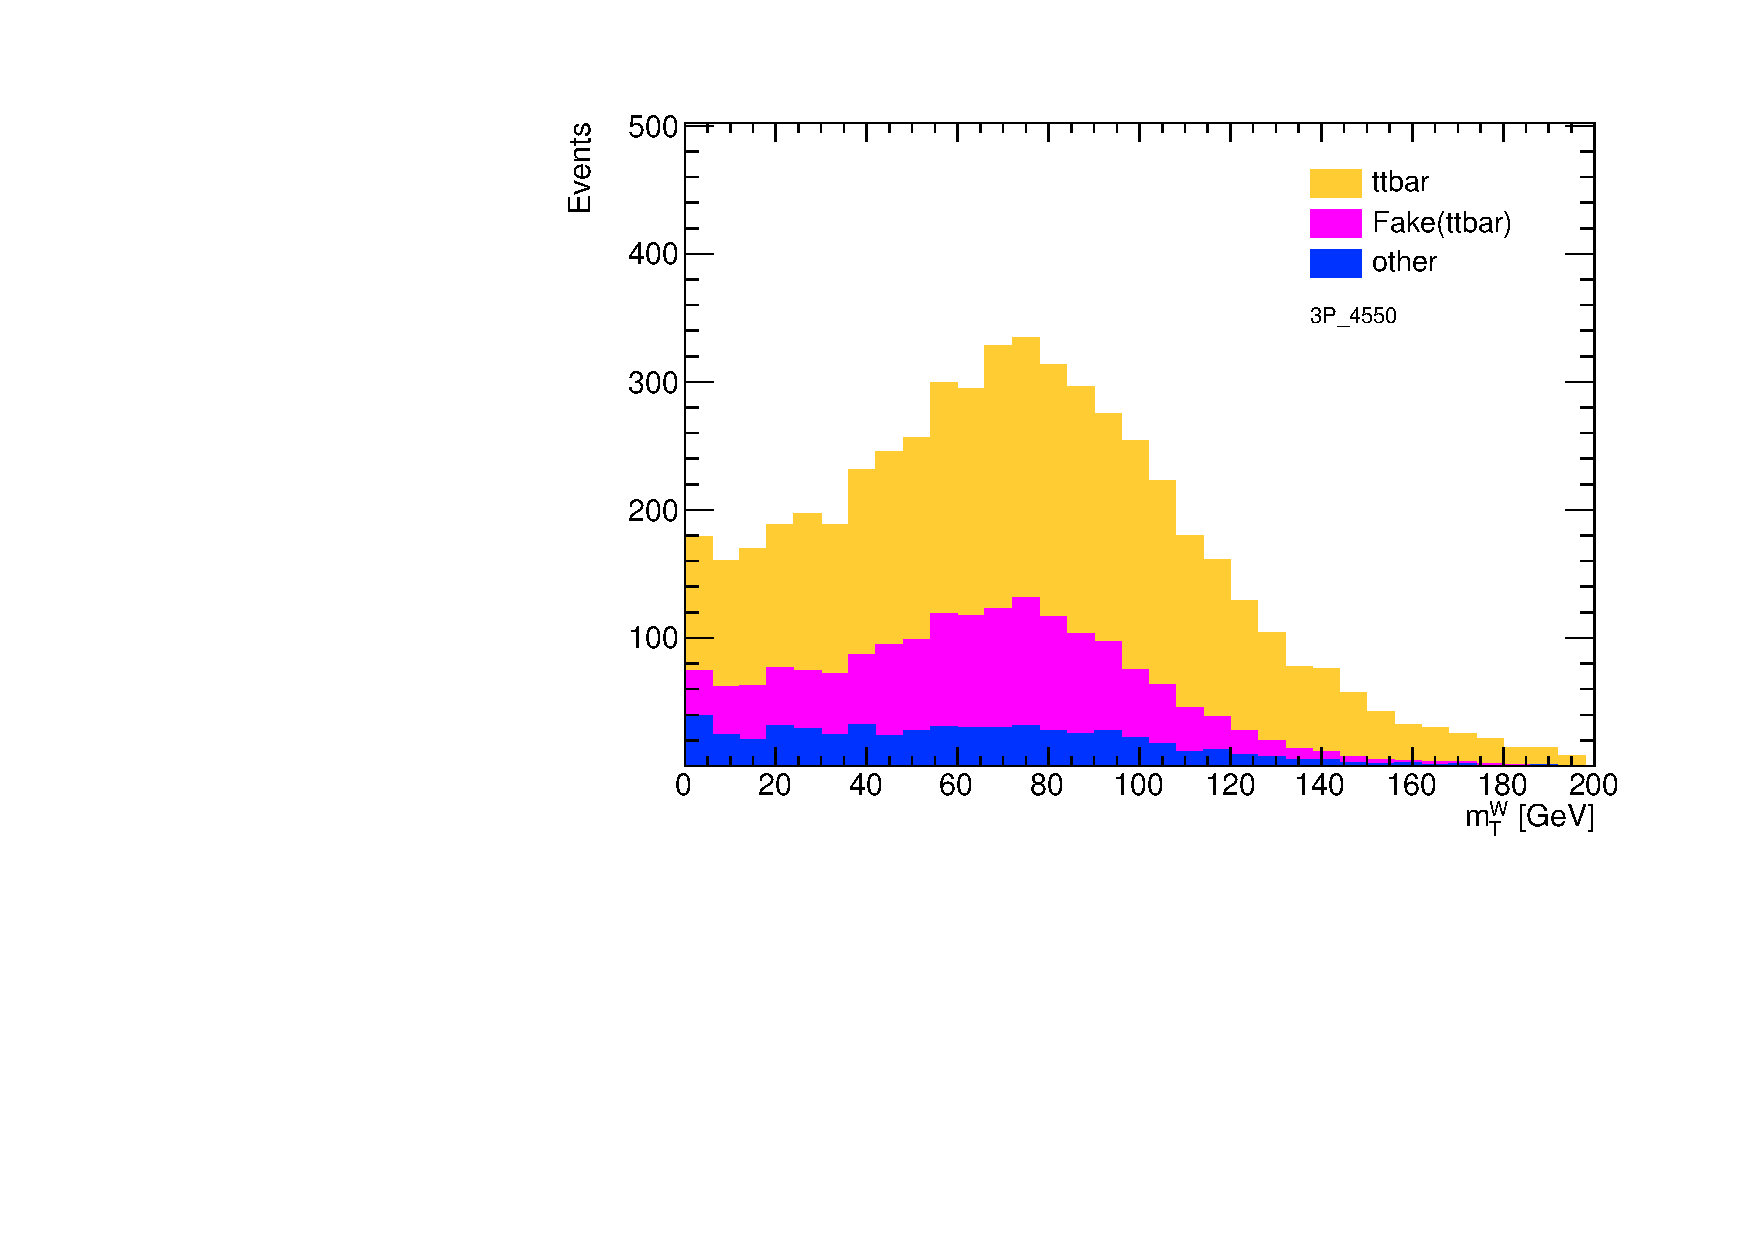
\includegraphics[scale=0.15]{mtw_fine_binning_stLT400_3P_4550}} \\
        \subfloat[$50<p_T<55$] {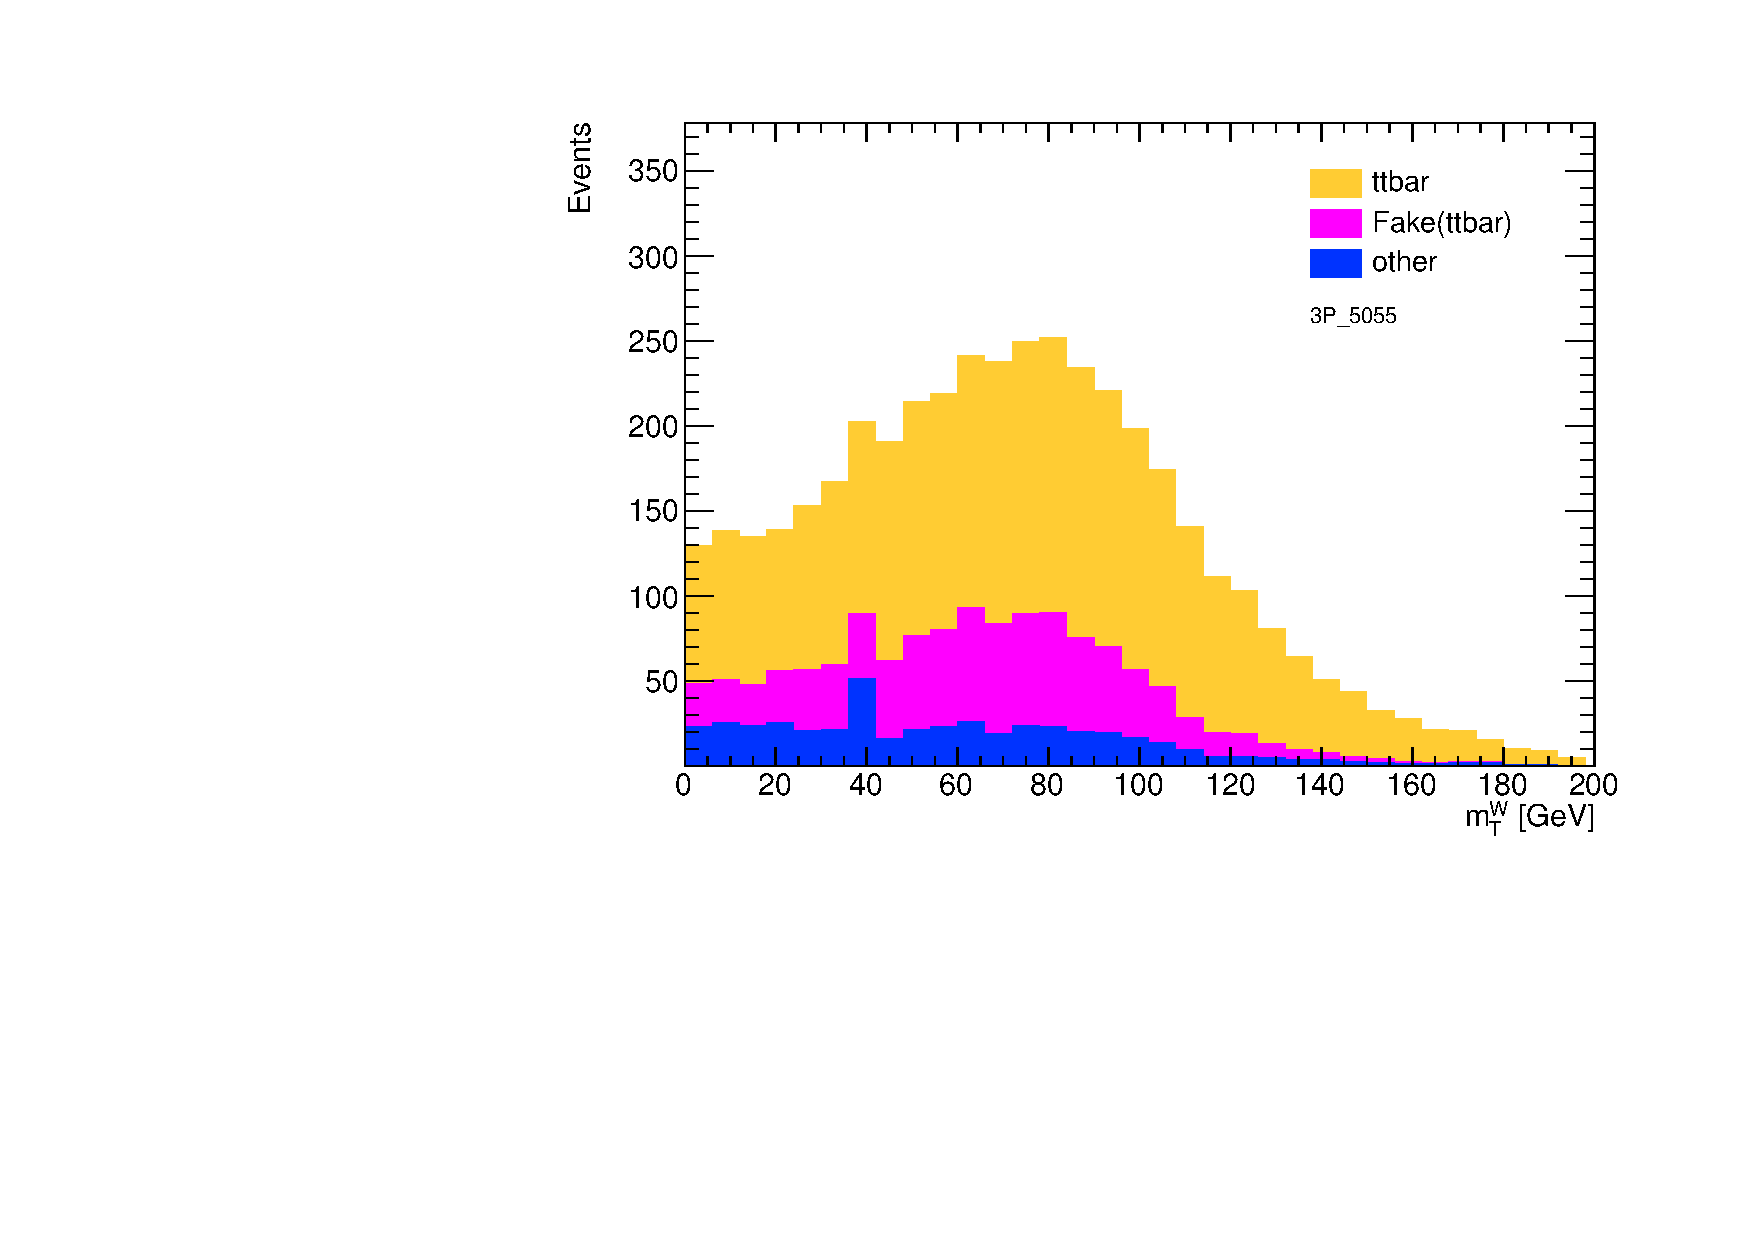
\includegraphics[scale=0.15]{mtw_fine_binning_stLT400_3P_5055}}
        \subfloat[$55<p_T<70$] {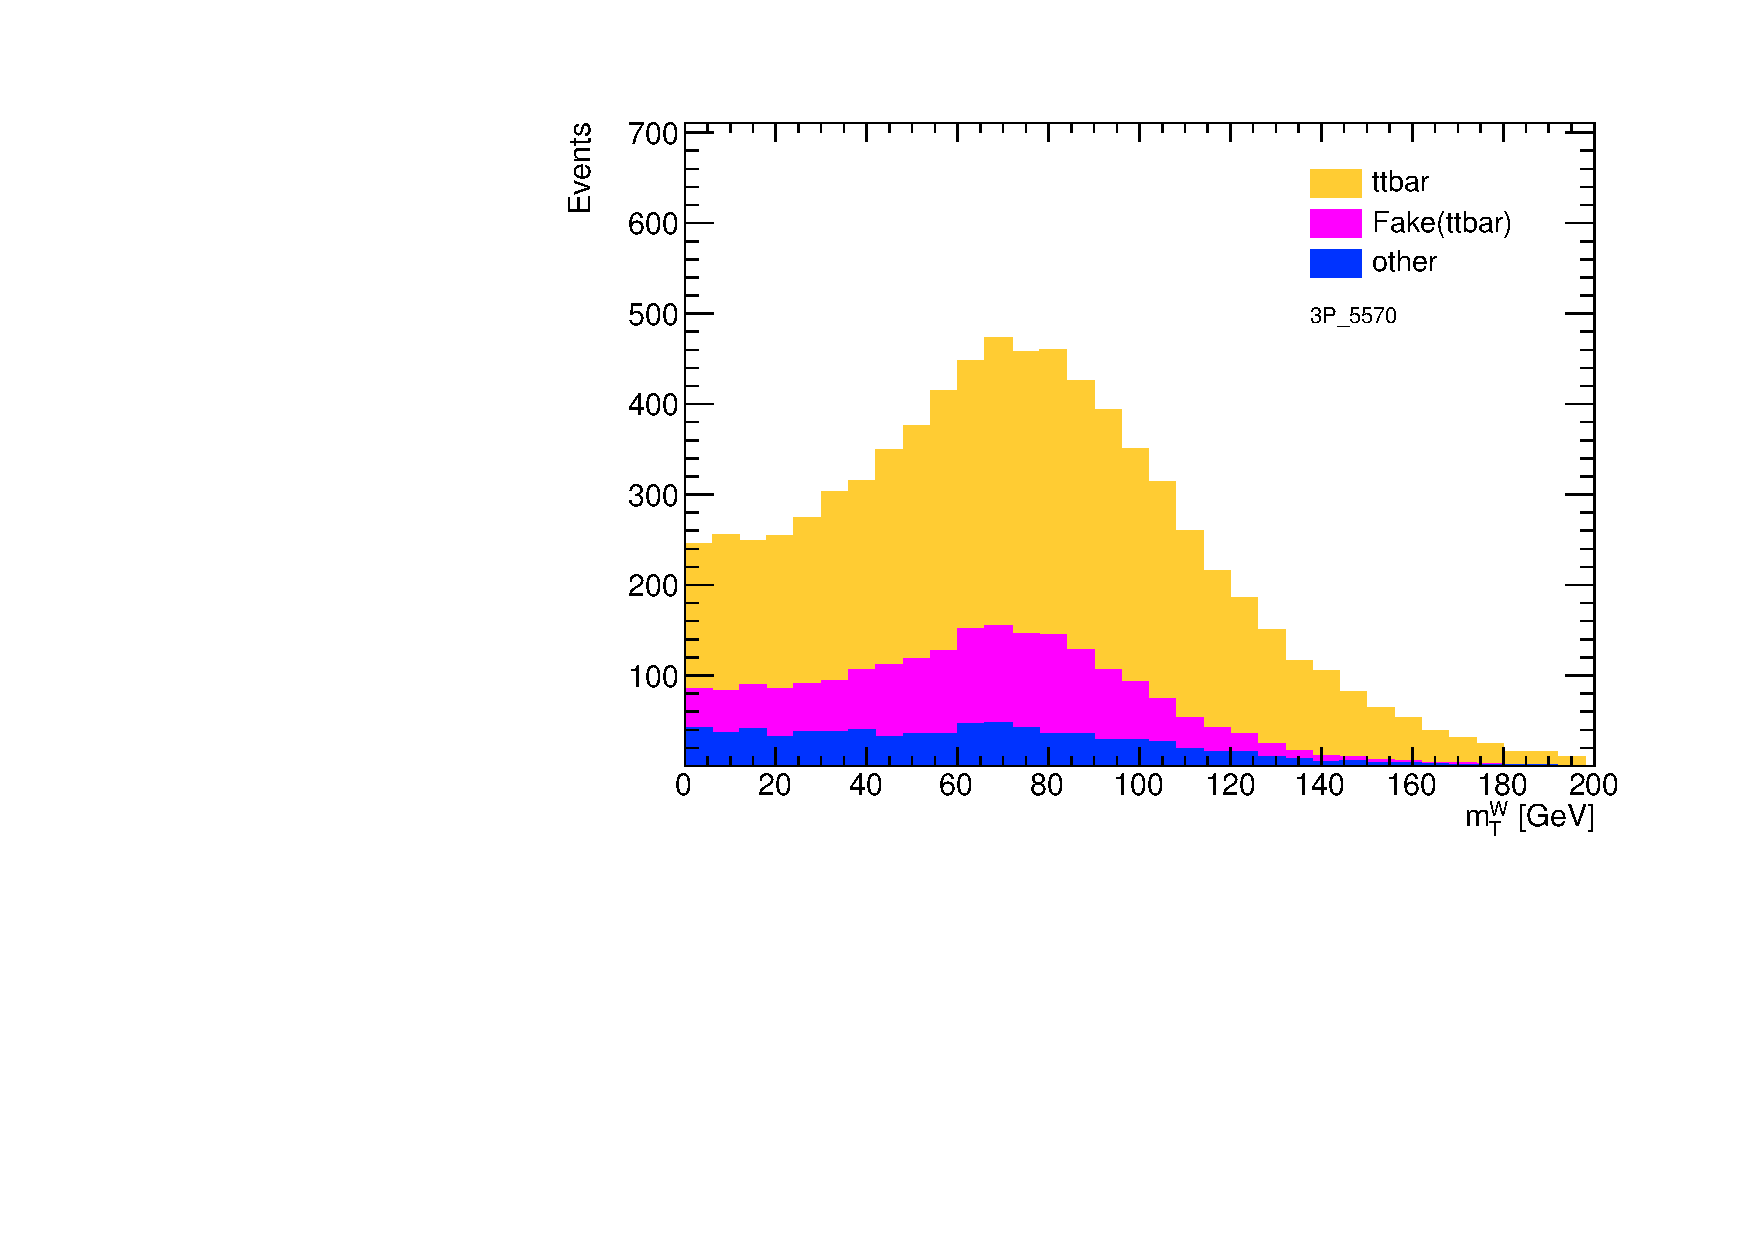
\includegraphics[scale=0.15]{mtw_fine_binning_stLT400_3P_5570}}
        \subfloat[$70<p_T$]    {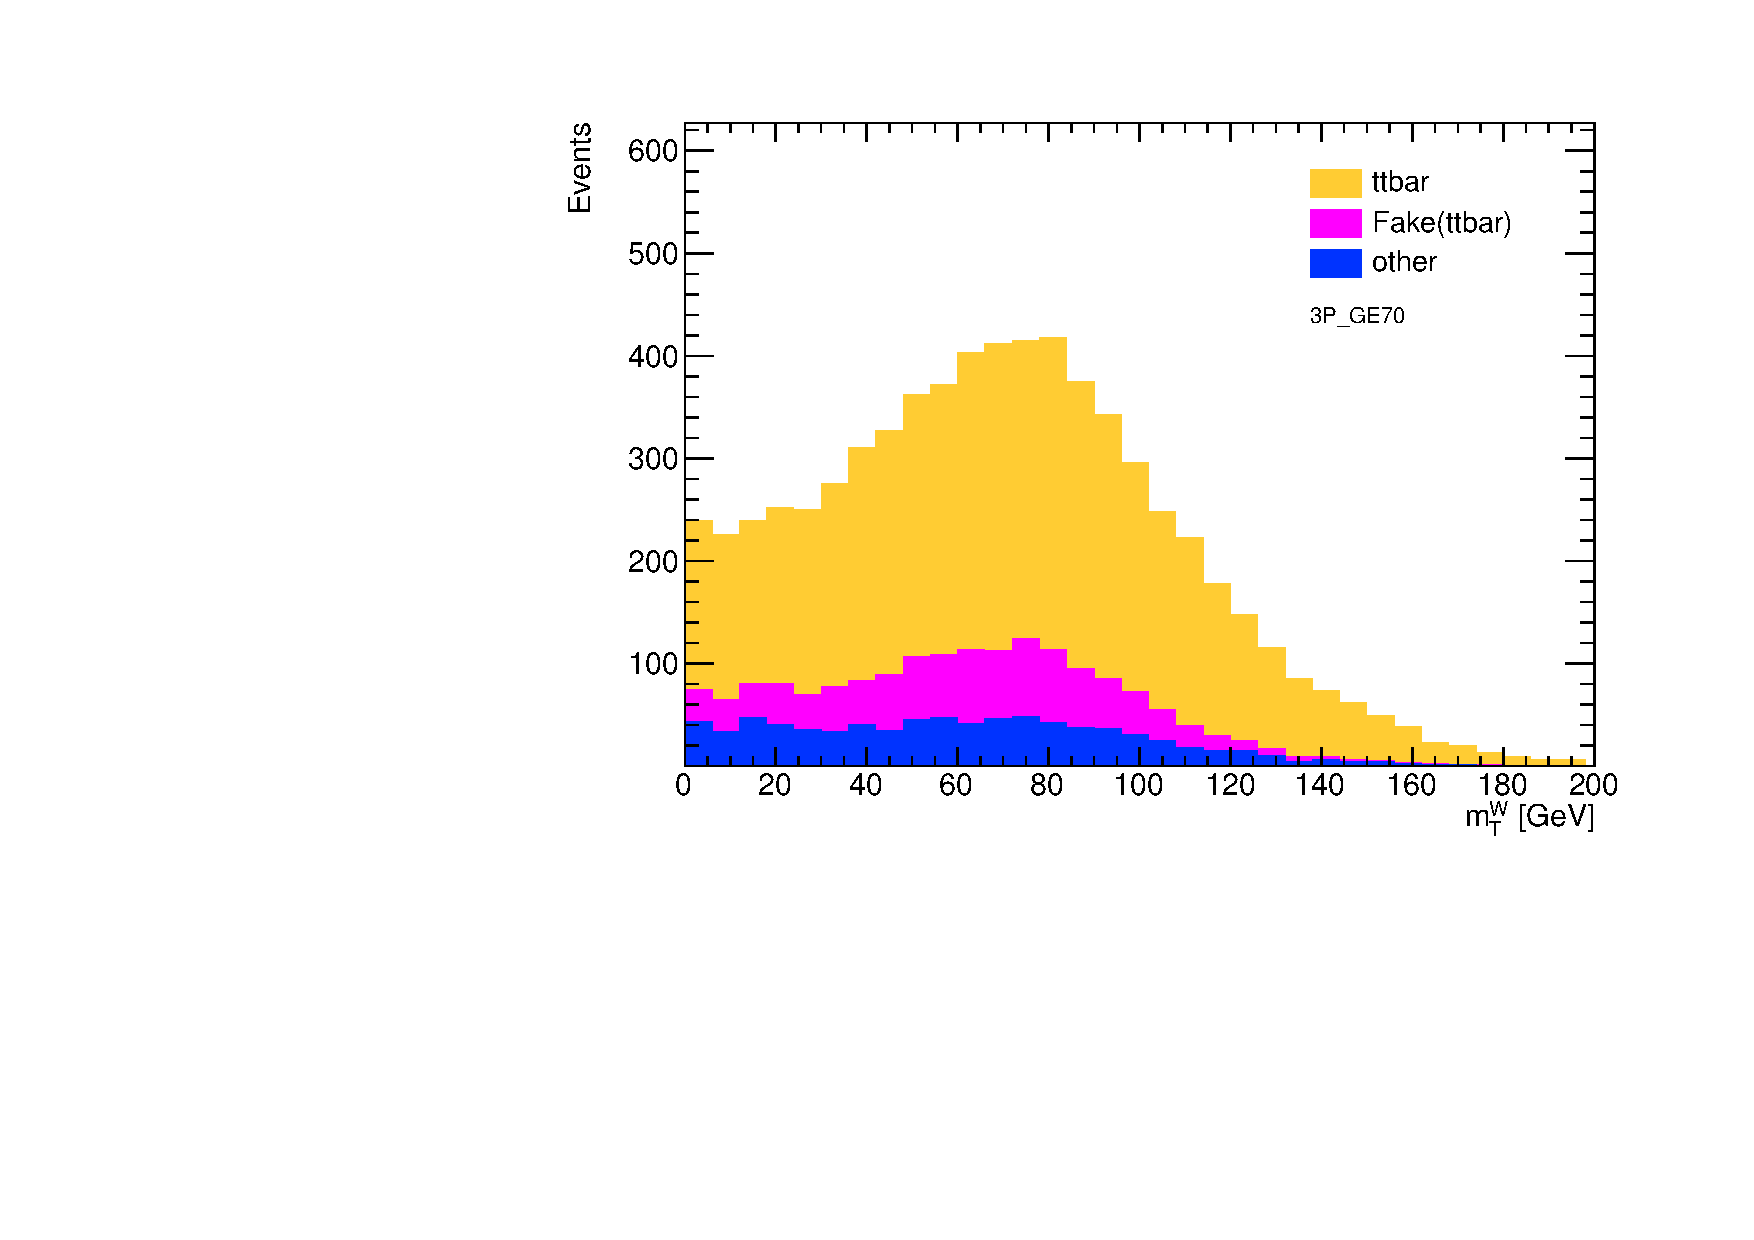
\includegraphics[scale=0.15]{mtw_fine_binning_stLT400_3P_GE70}}
  \end{figure}       
\end{frame}


\begin{frame}{\mtw distribution (1-prong, CR2)}
  \begin{figure}
    \setcounter{subfigure}{0}
    \centering
        \subfloat[$p_T<35$]    {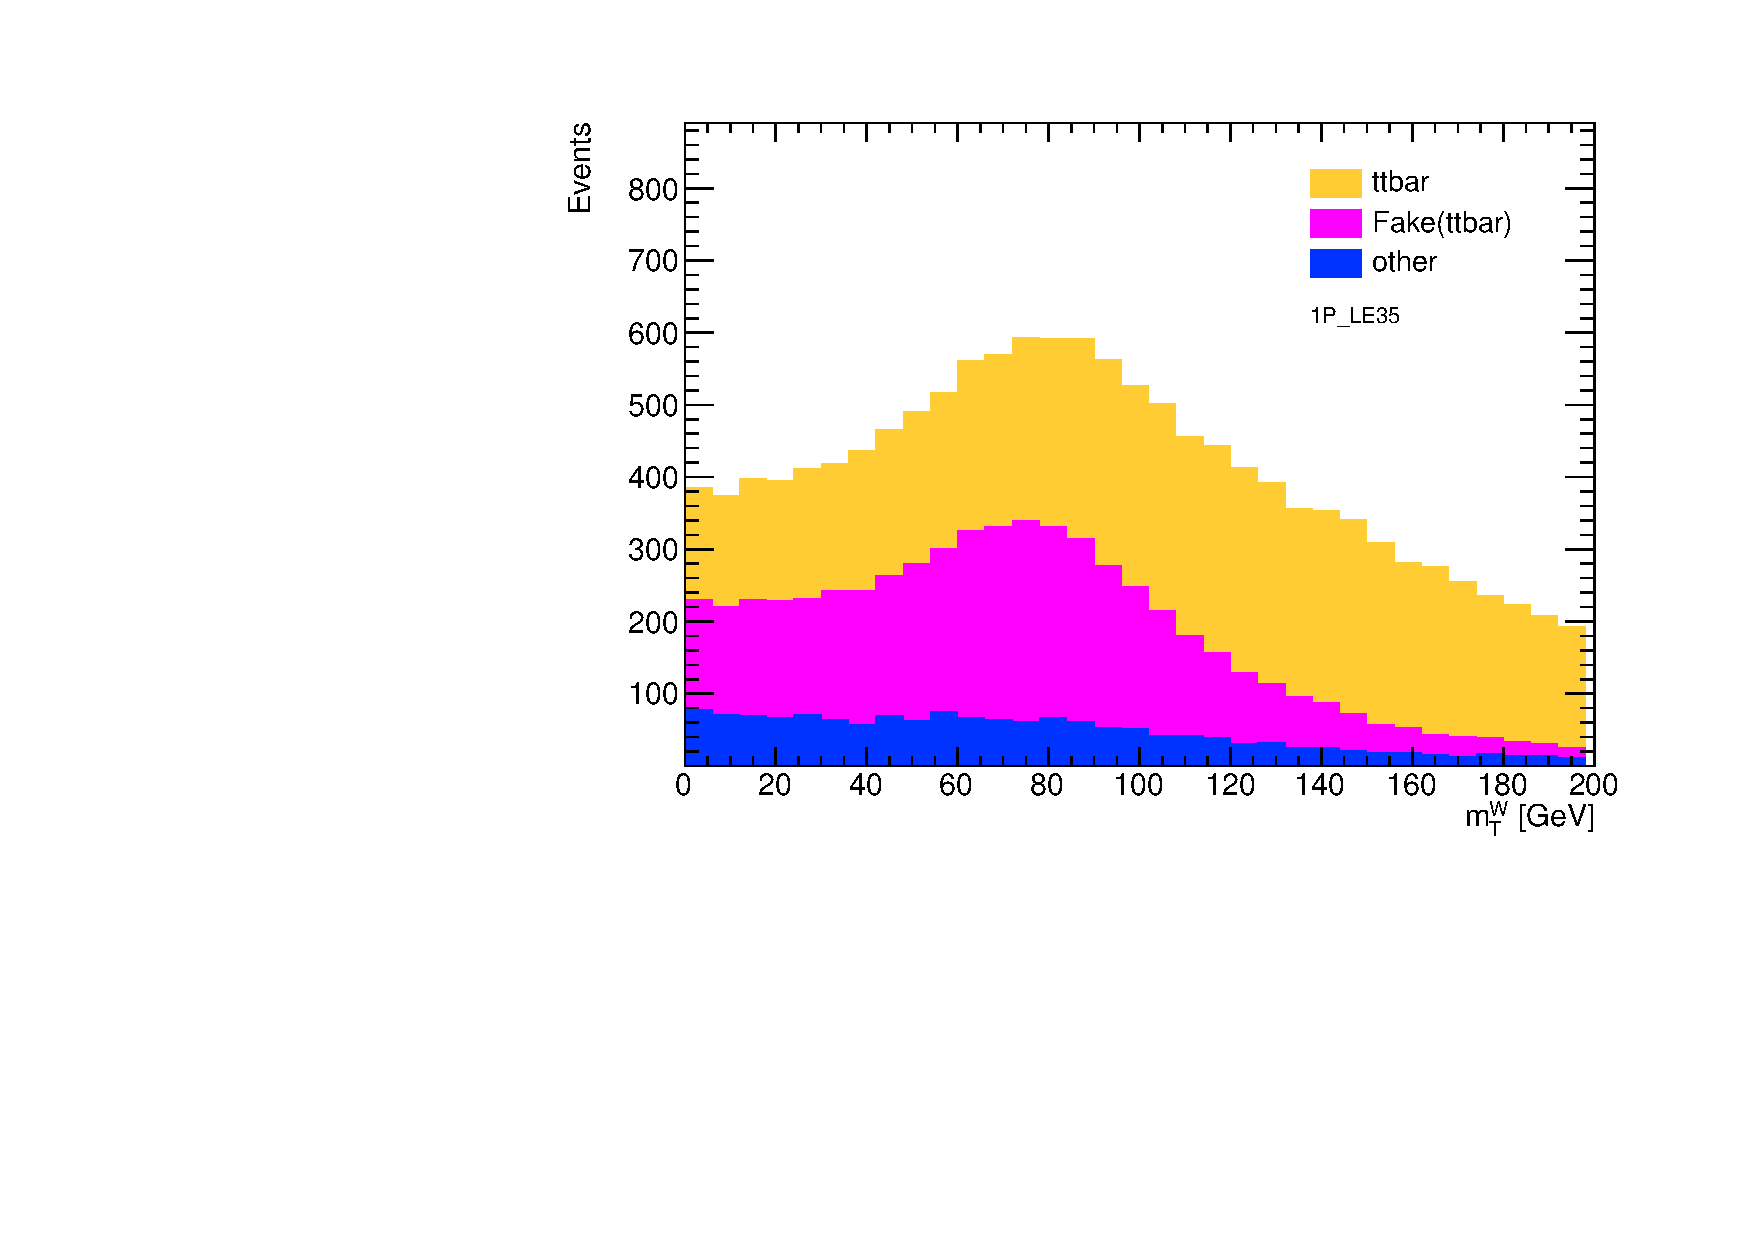
\includegraphics[scale=0.15]{mtw_fine_binning_stGE400LT500_1P_LE35}}
        \subfloat[$35<p_T<40$] {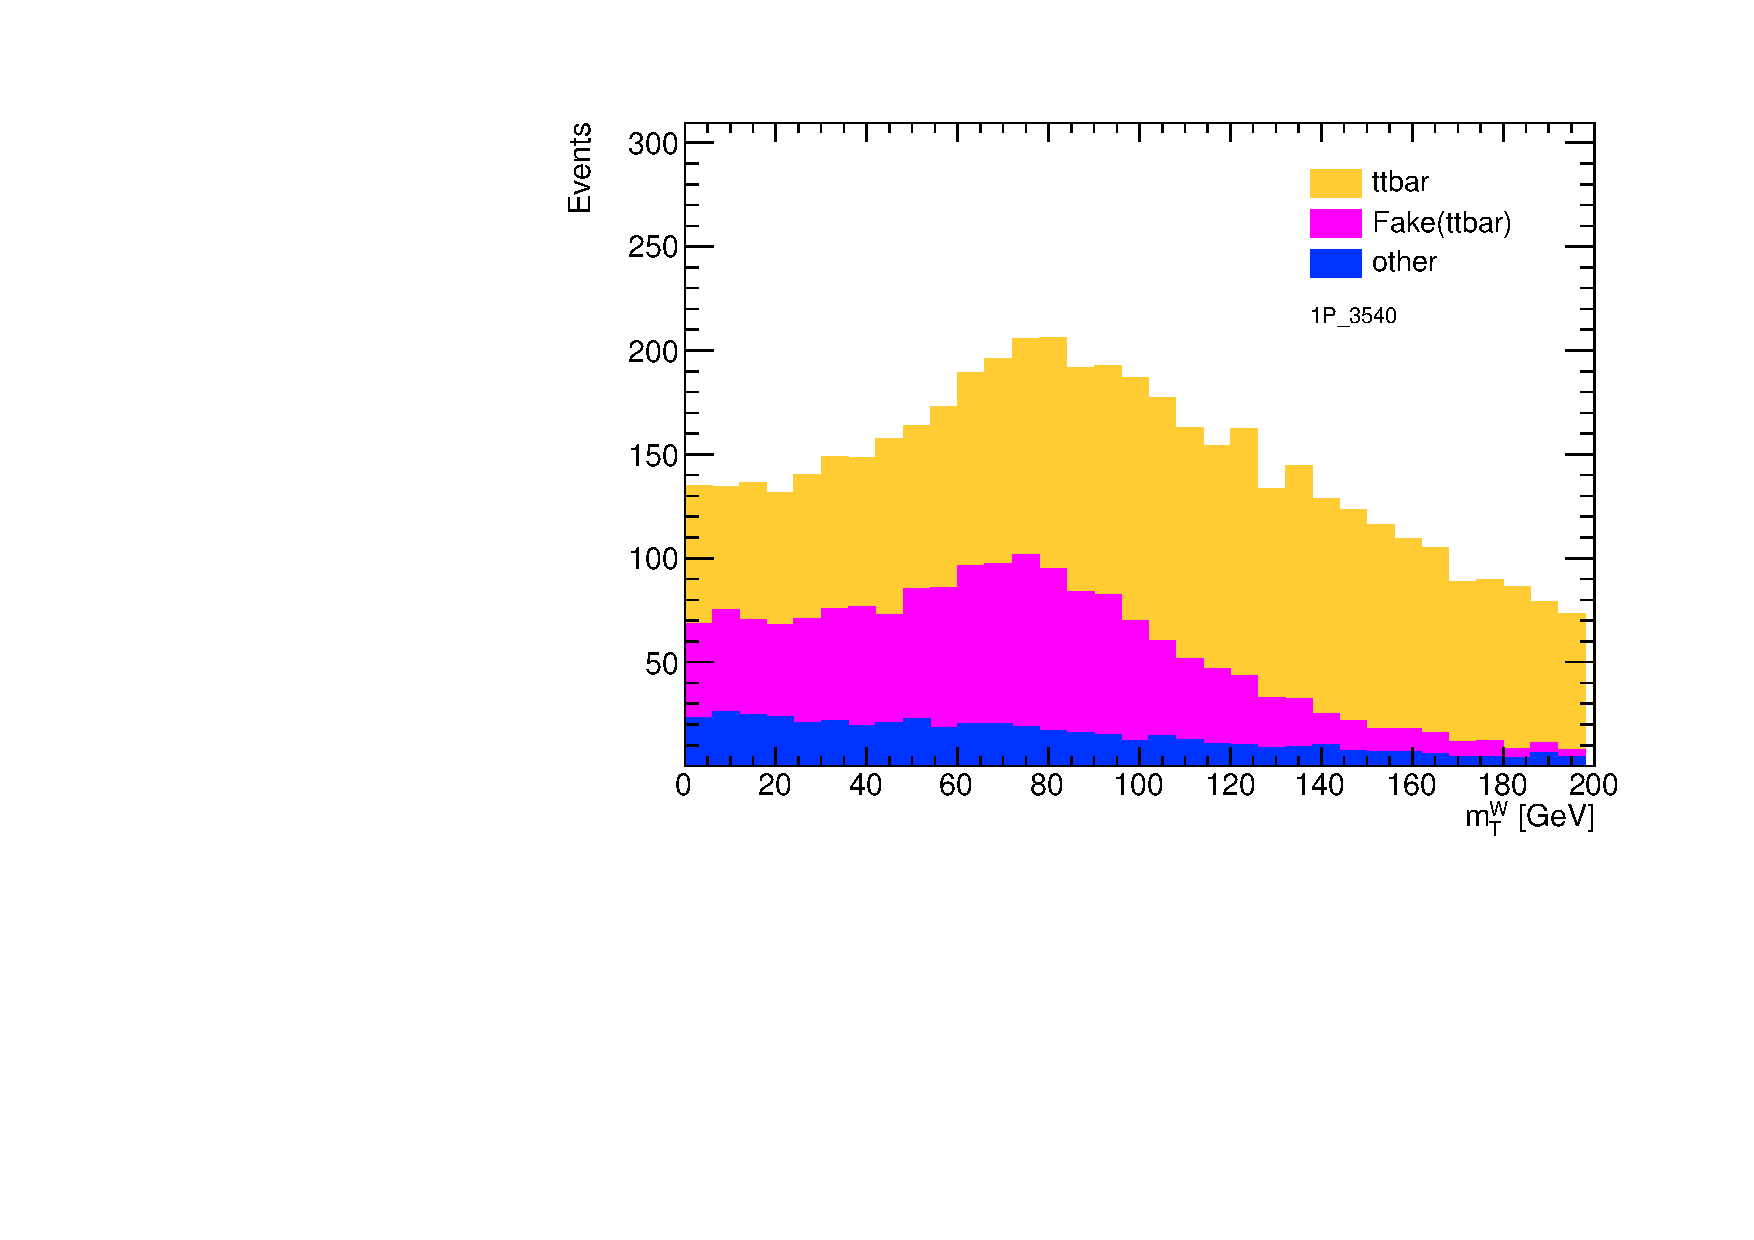
\includegraphics[scale=0.15]{mtw_fine_binning_stGE400LT500_1P_3540}}
        \subfloat[$40<p_T<45$] {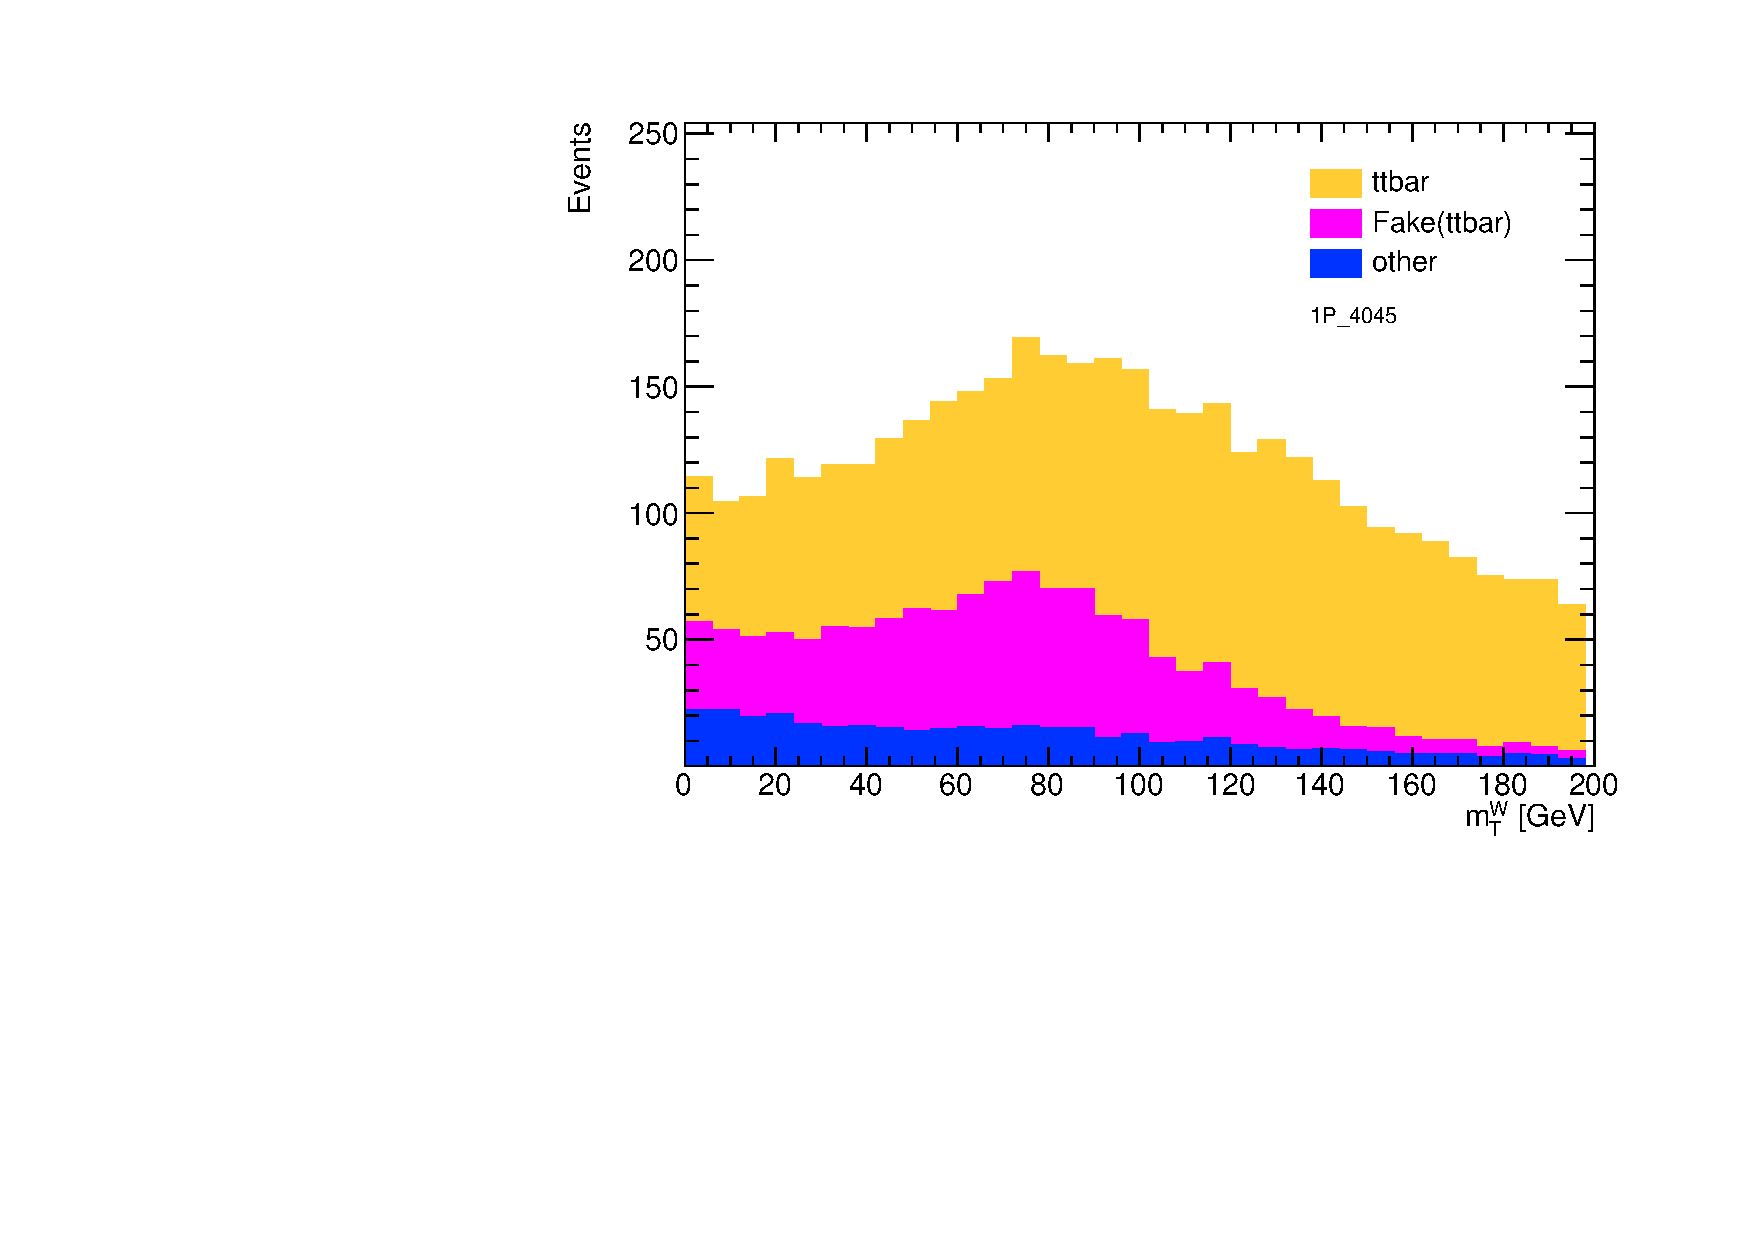
\includegraphics[scale=0.15]{mtw_fine_binning_stGE400LT500_1P_4045}}
        \subfloat[$45<p_T<50$] {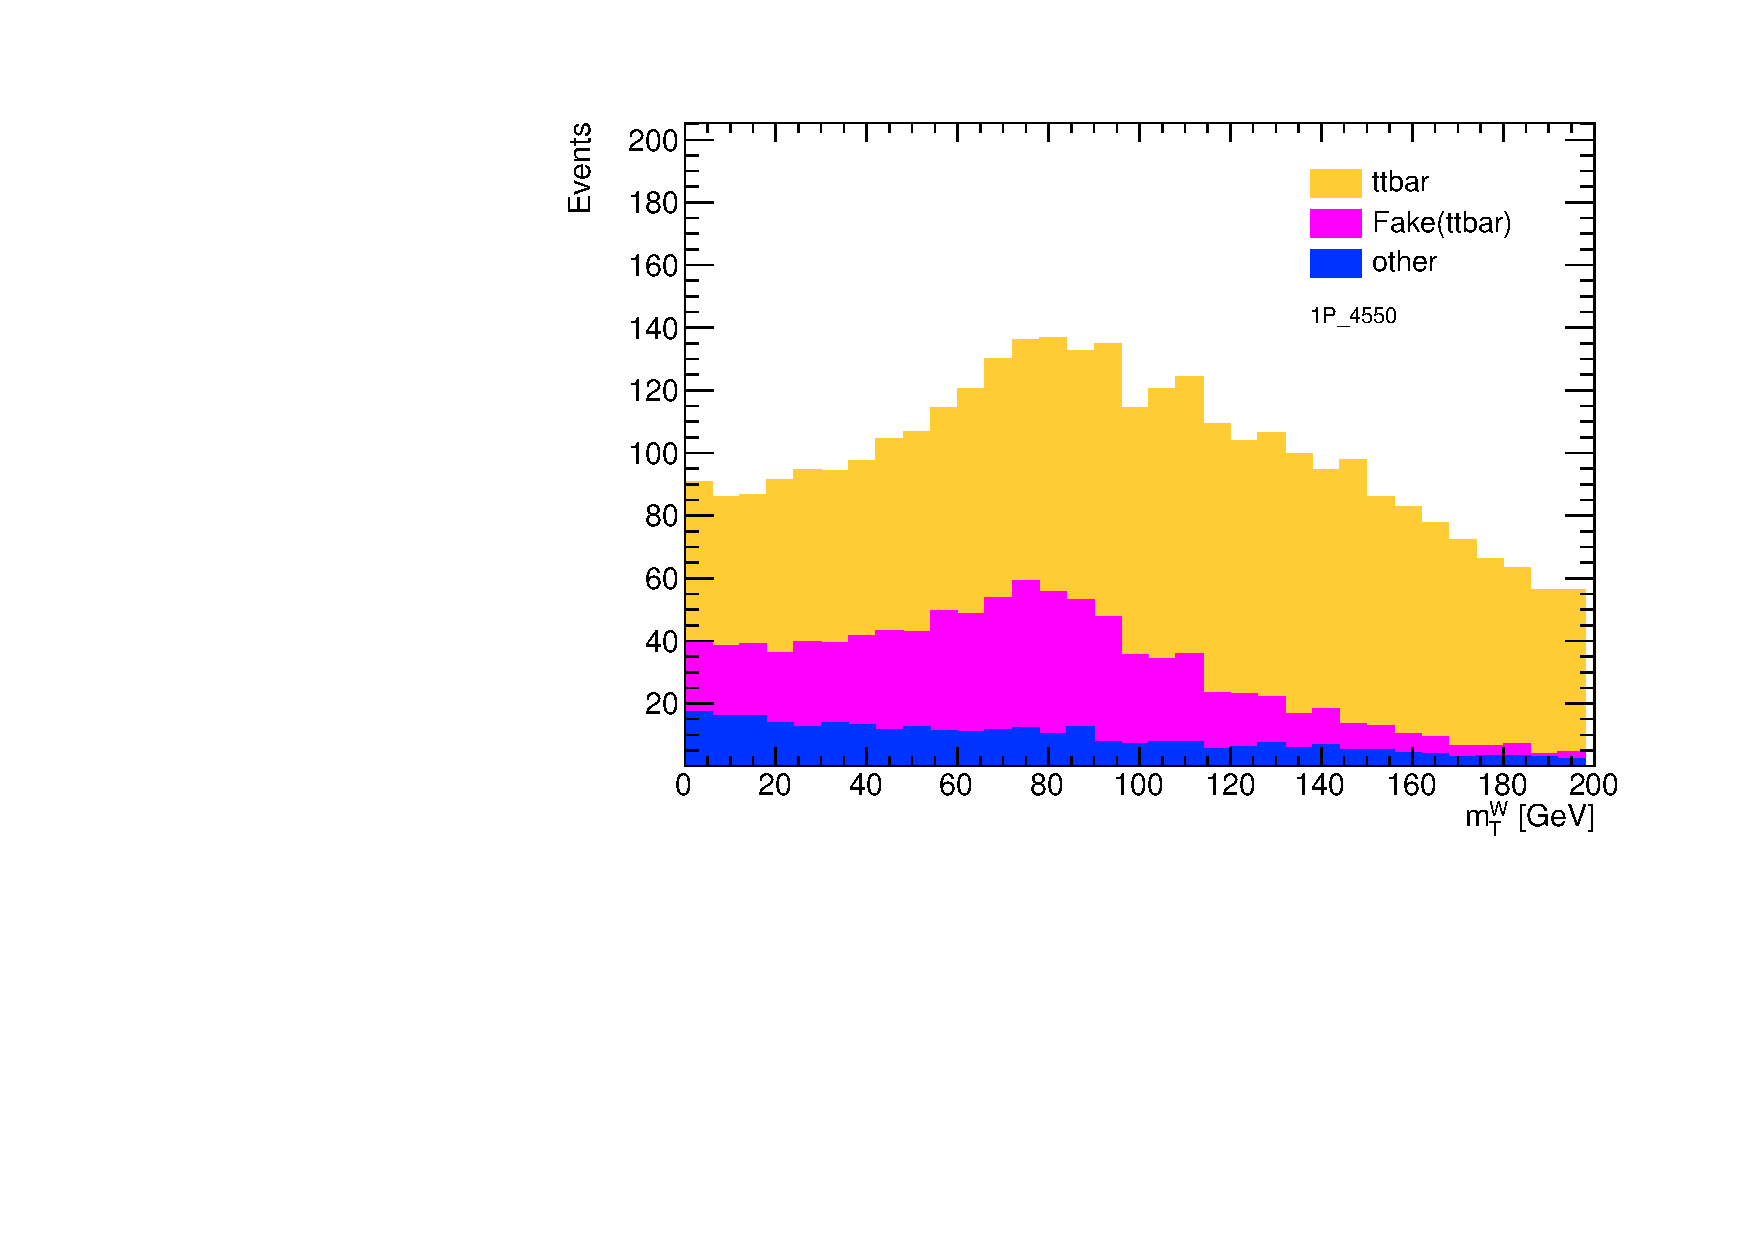
\includegraphics[scale=0.15]{mtw_fine_binning_stGE400LT500_1P_4550}} \\
        \subfloat[$50<p_T<55$] {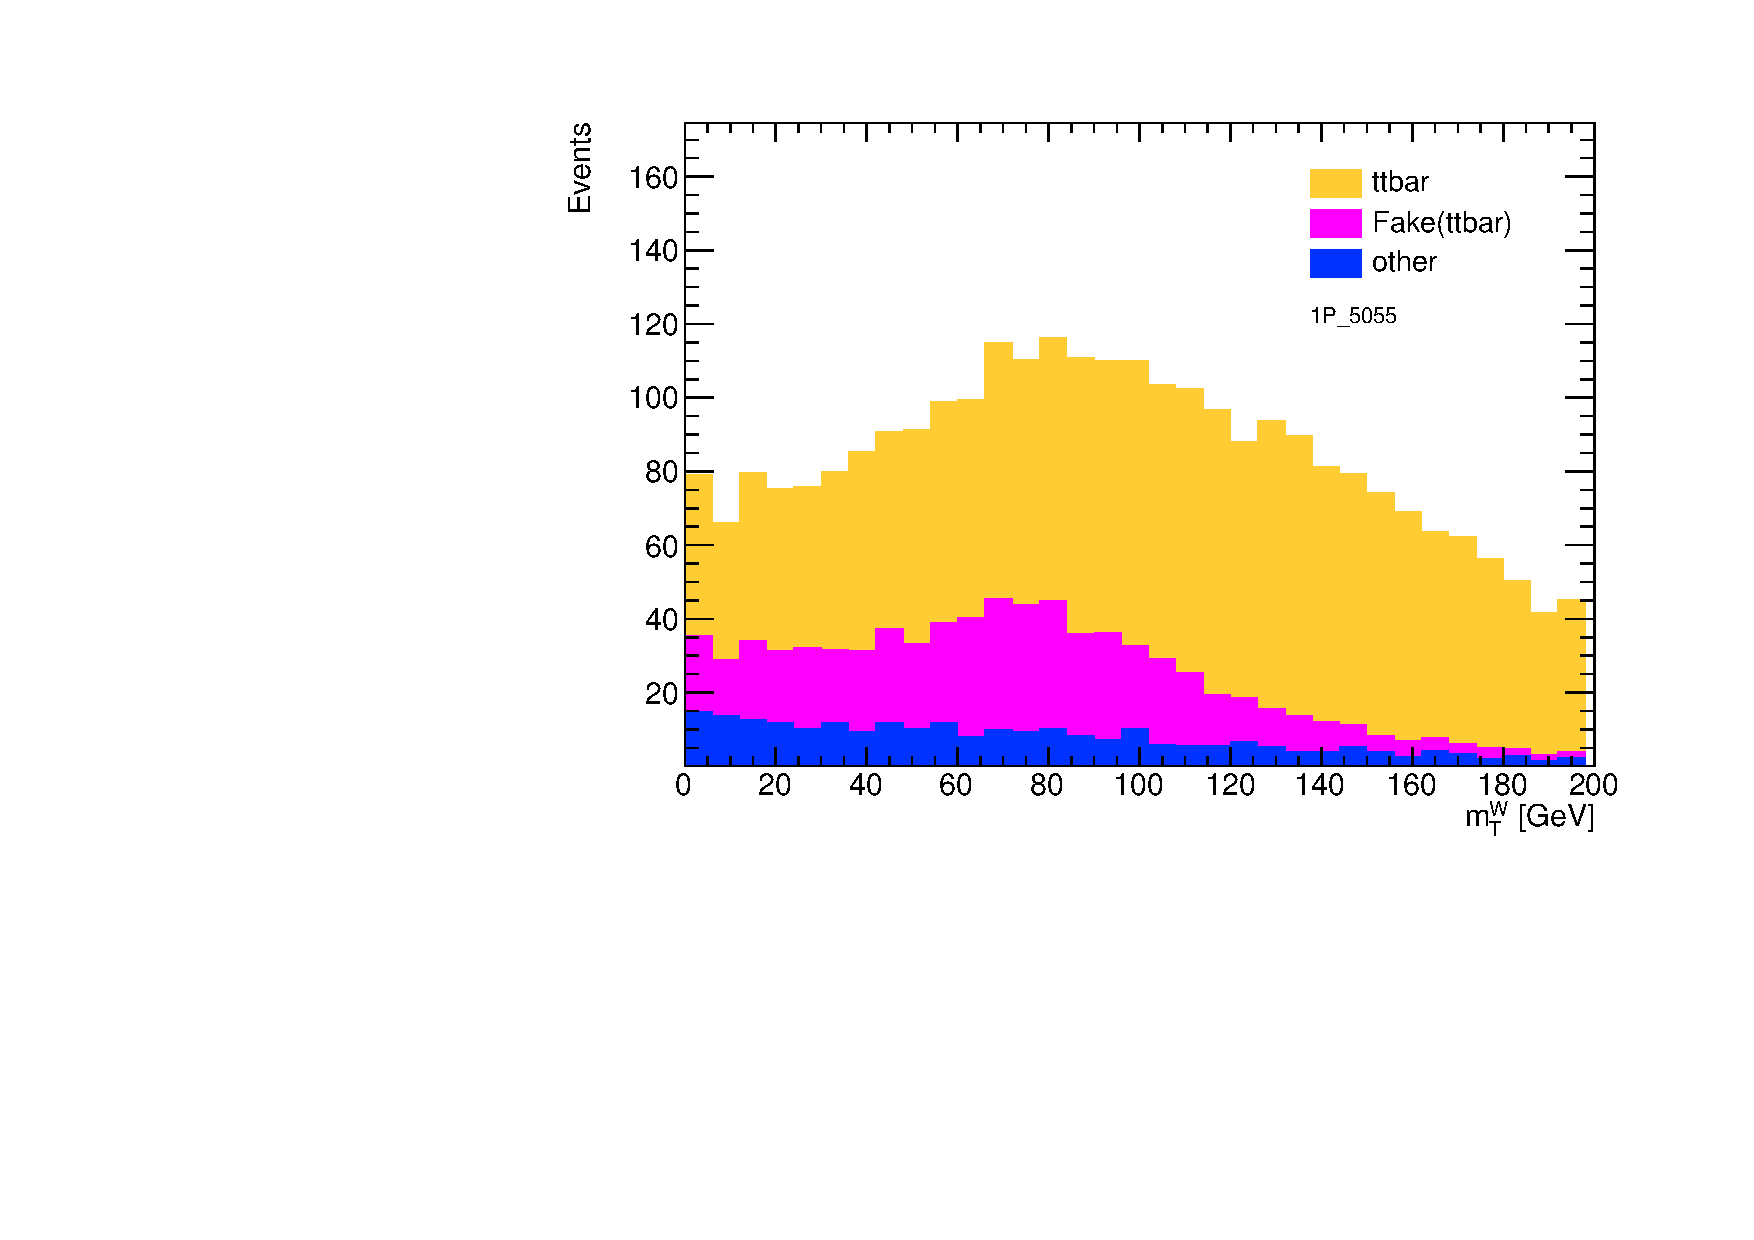
\includegraphics[scale=0.15]{mtw_fine_binning_stGE400LT500_1P_5055}}
        \subfloat[$55<p_T<70$] {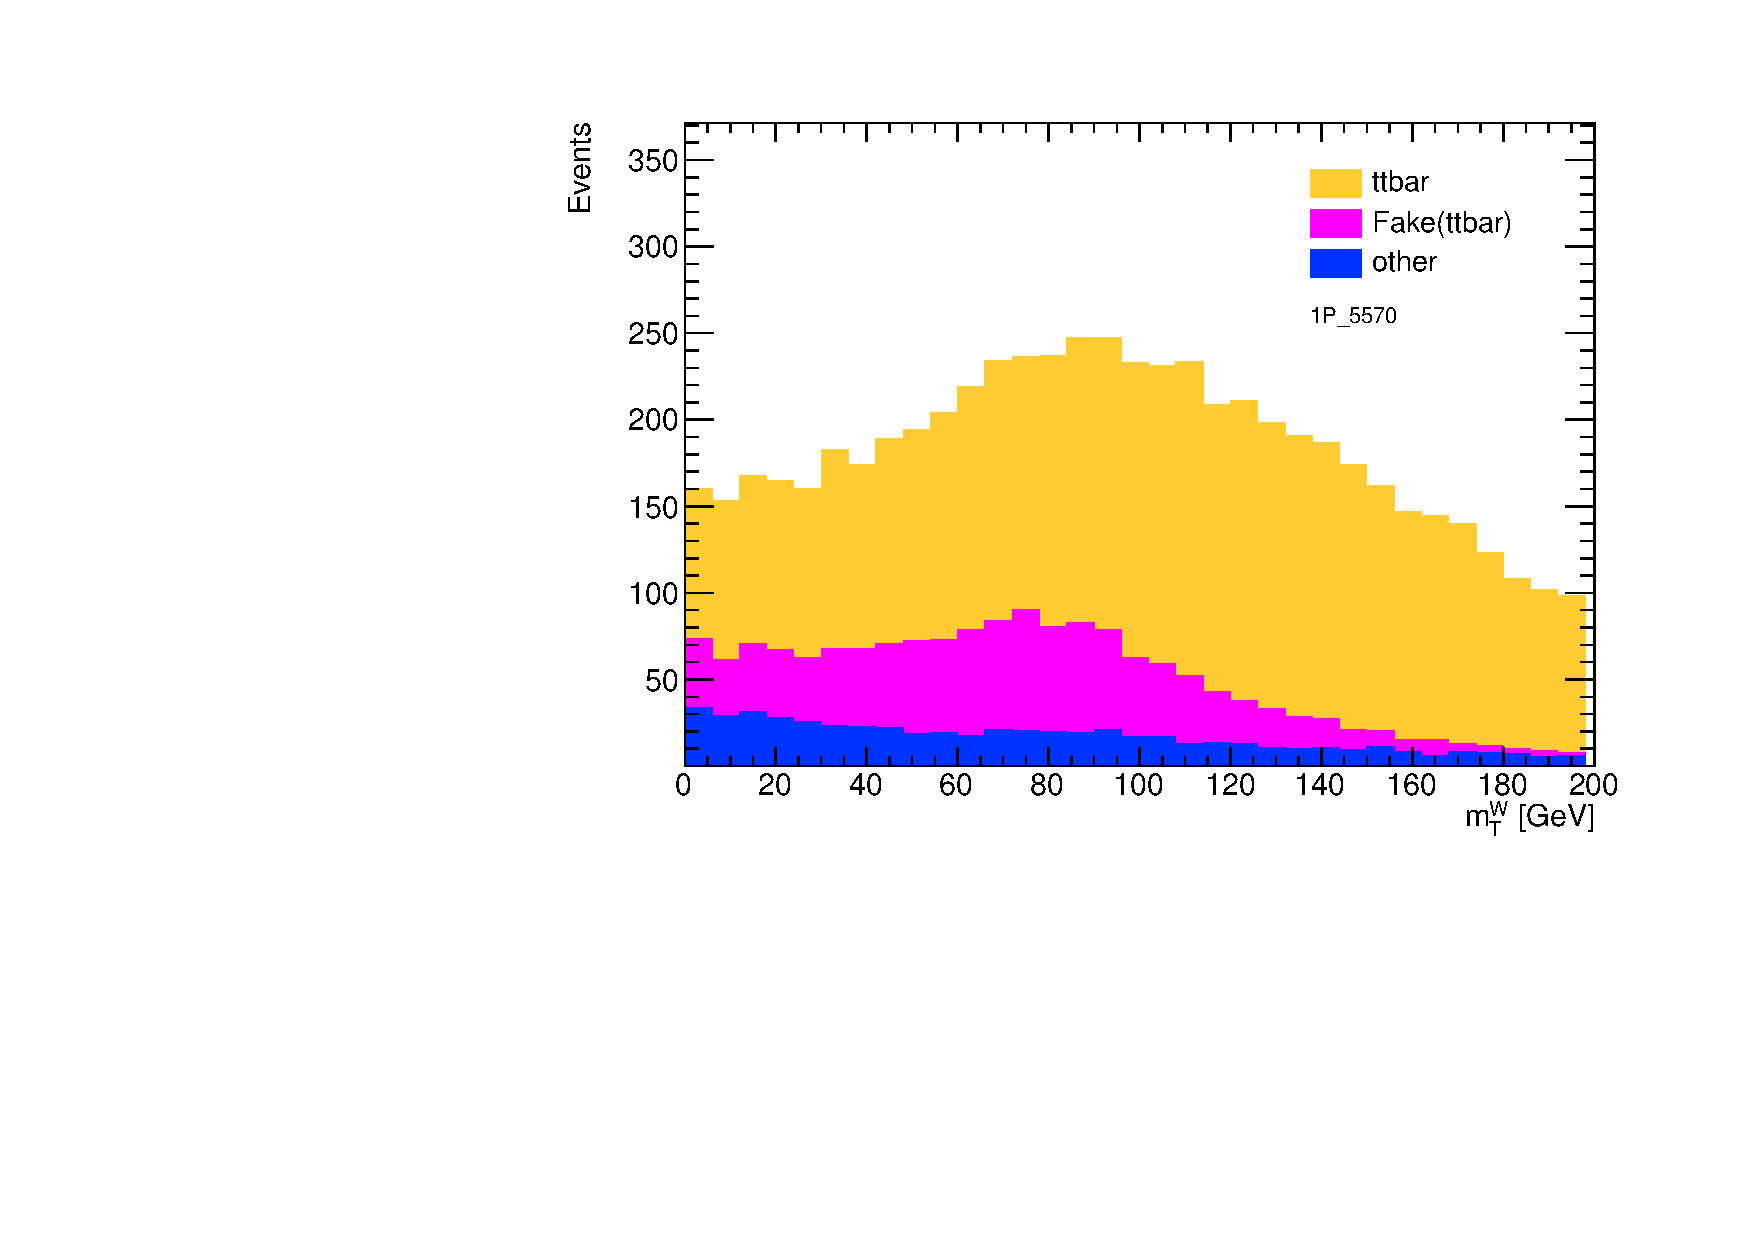
\includegraphics[scale=0.15]{mtw_fine_binning_stGE400LT500_1P_5570}}
        \subfloat[$70<p_T<100$]{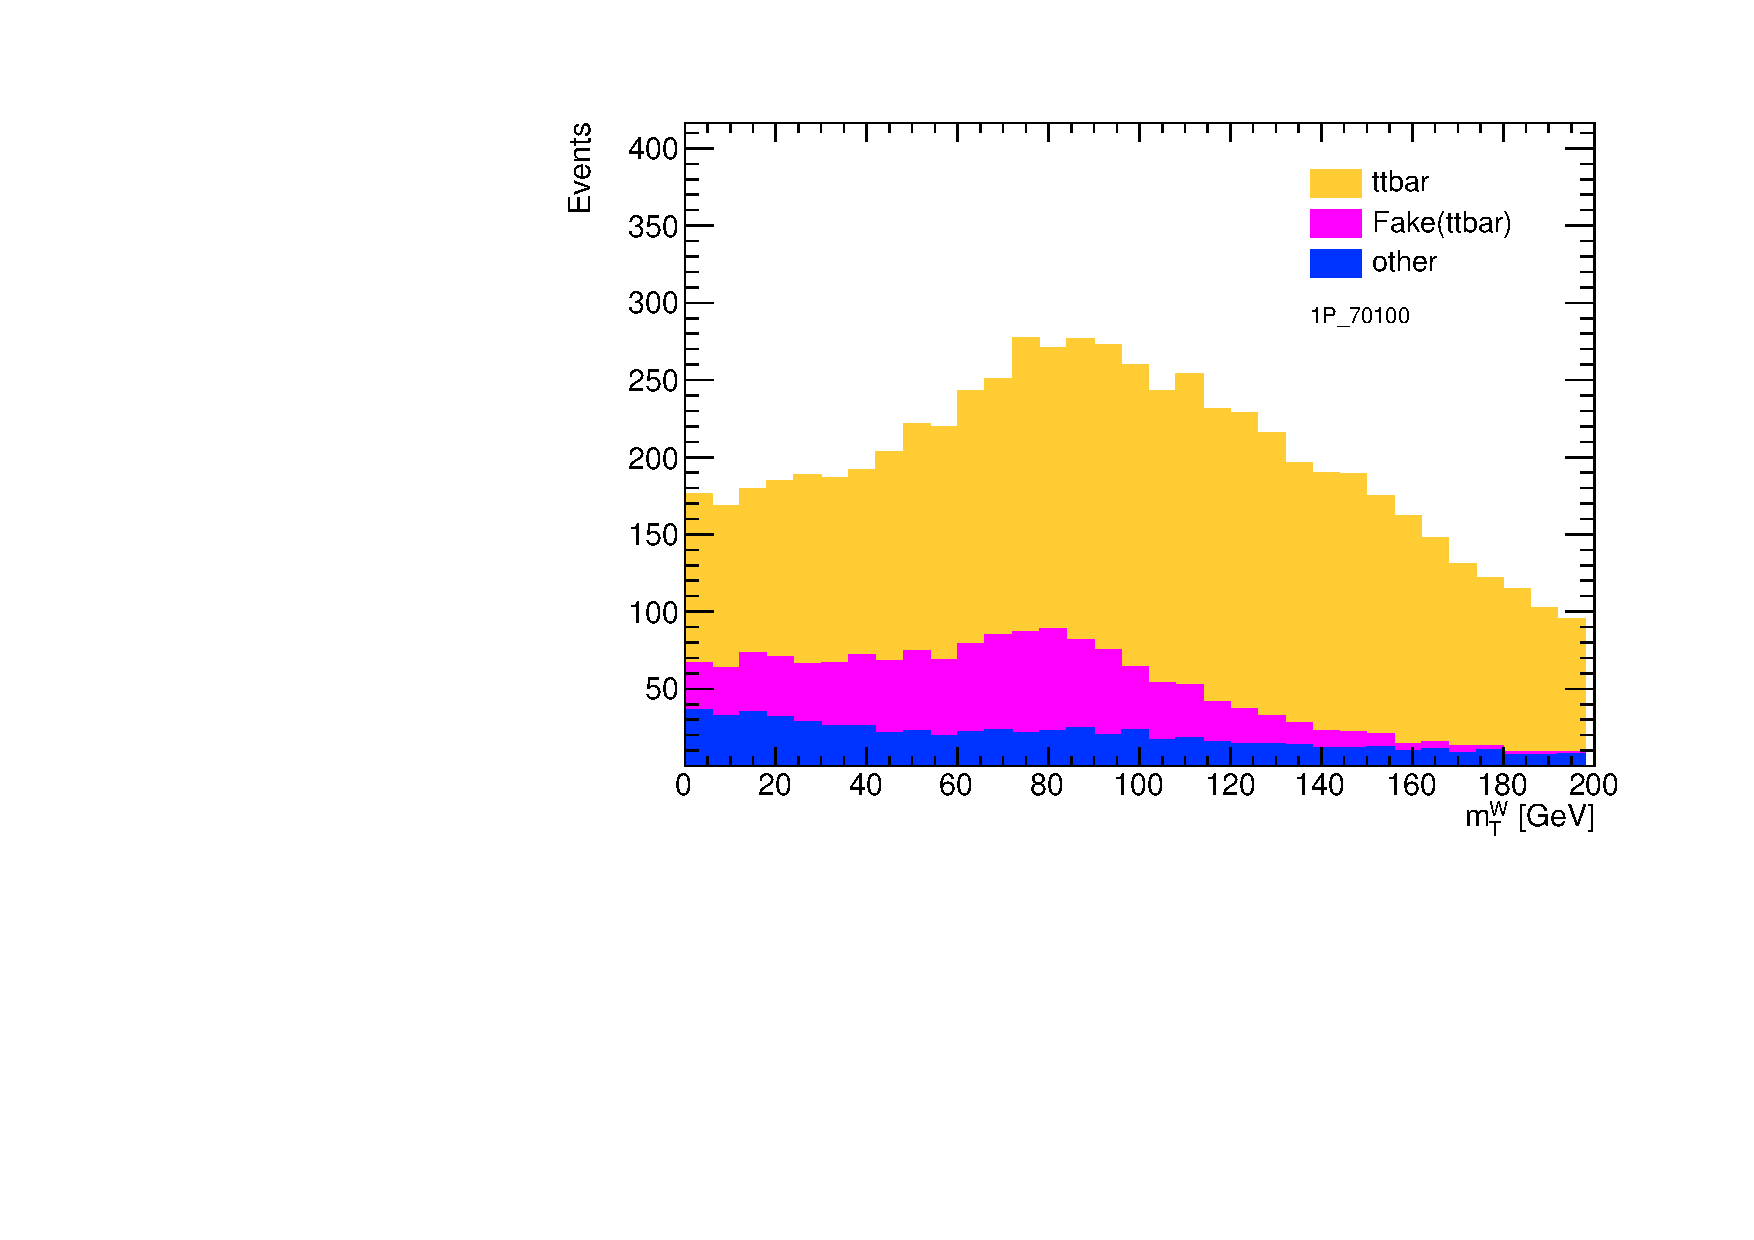
\includegraphics[scale=0.15]{mtw_fine_binning_stGE400LT500_1P_70100}}
        \subfloat[$100<p_T$]   {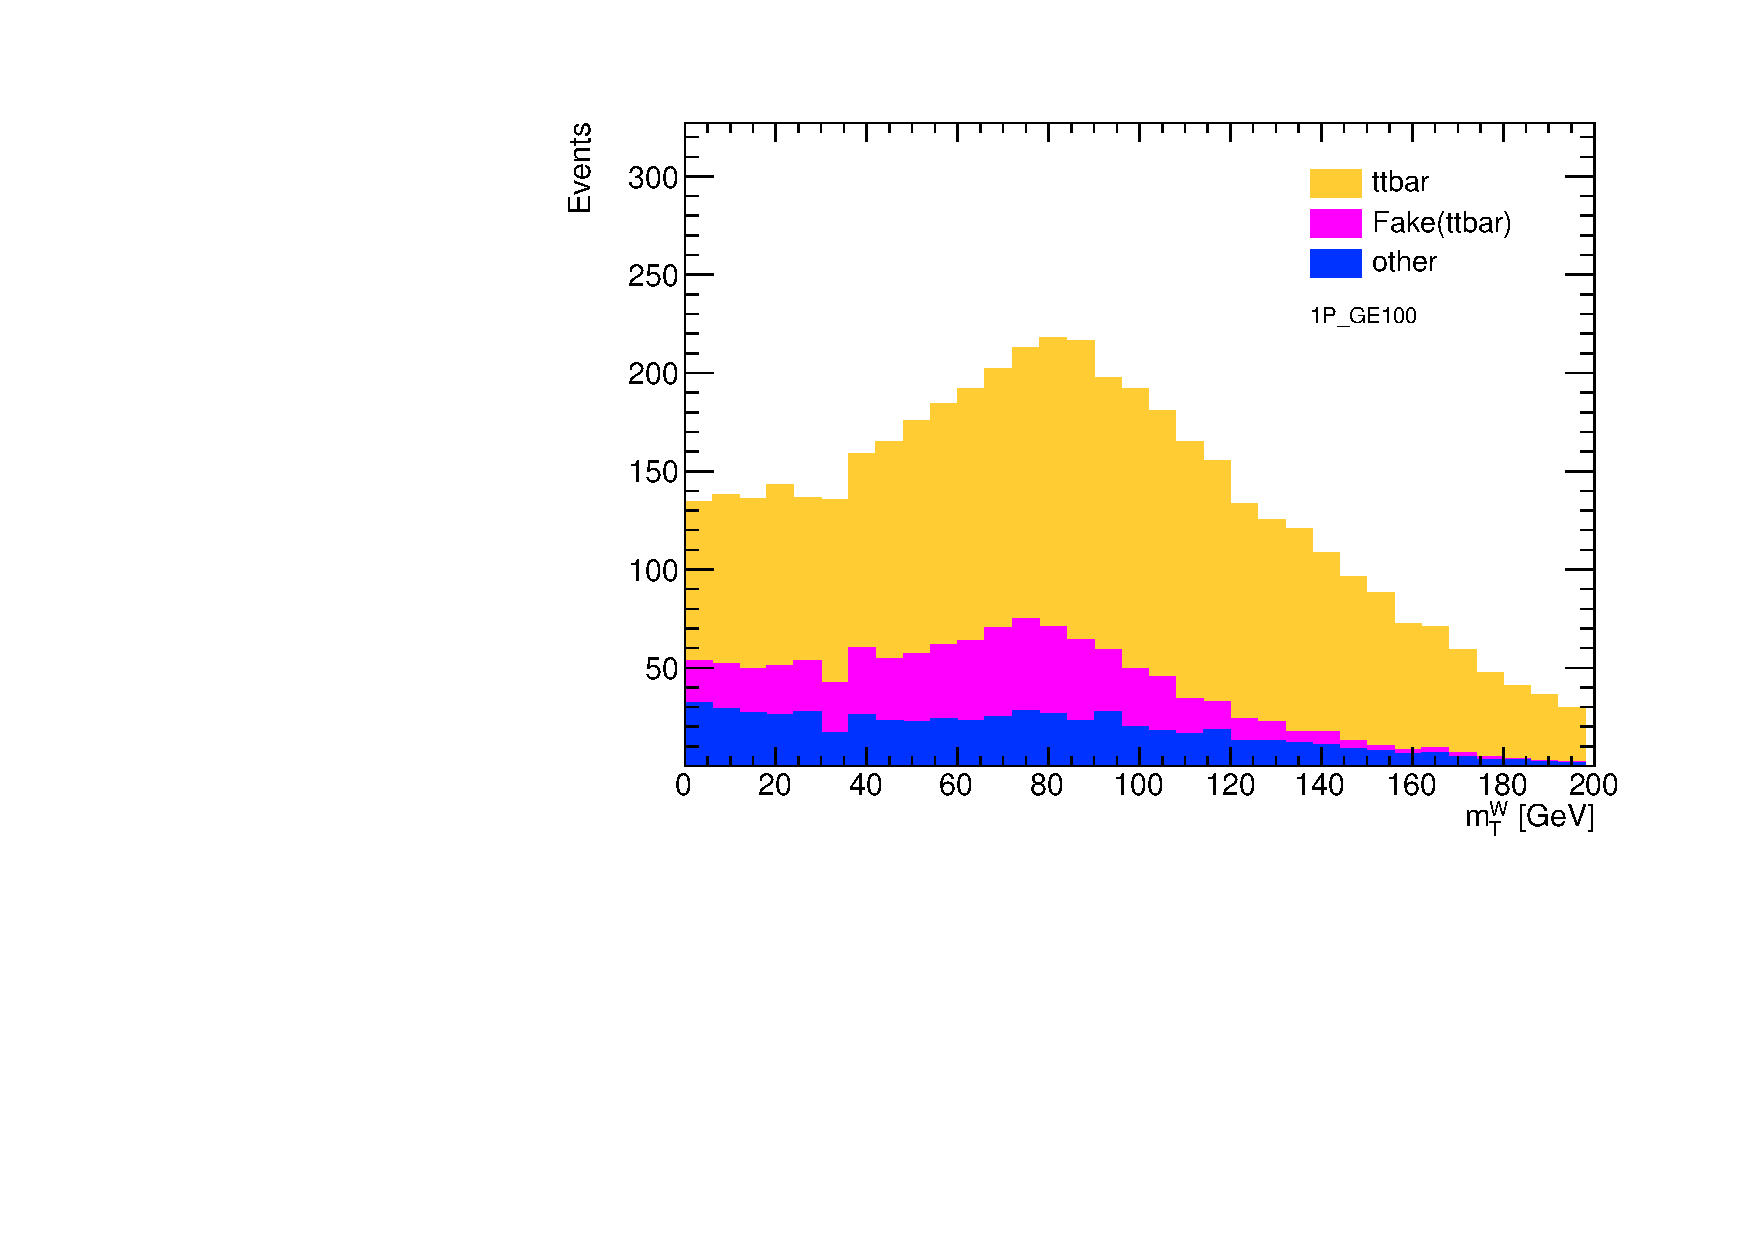
\includegraphics[scale=0.15]{mtw_fine_binning_stGE400LT500_1P_GE100}}\\
  \end{figure}
\end{frame}

\begin{frame}{\mtw distribution (3-prong, CR2)}
  \begin{figure}
    \setcounter{subfigure}{0}
    \centering
        \subfloat[$p_T<35$]    {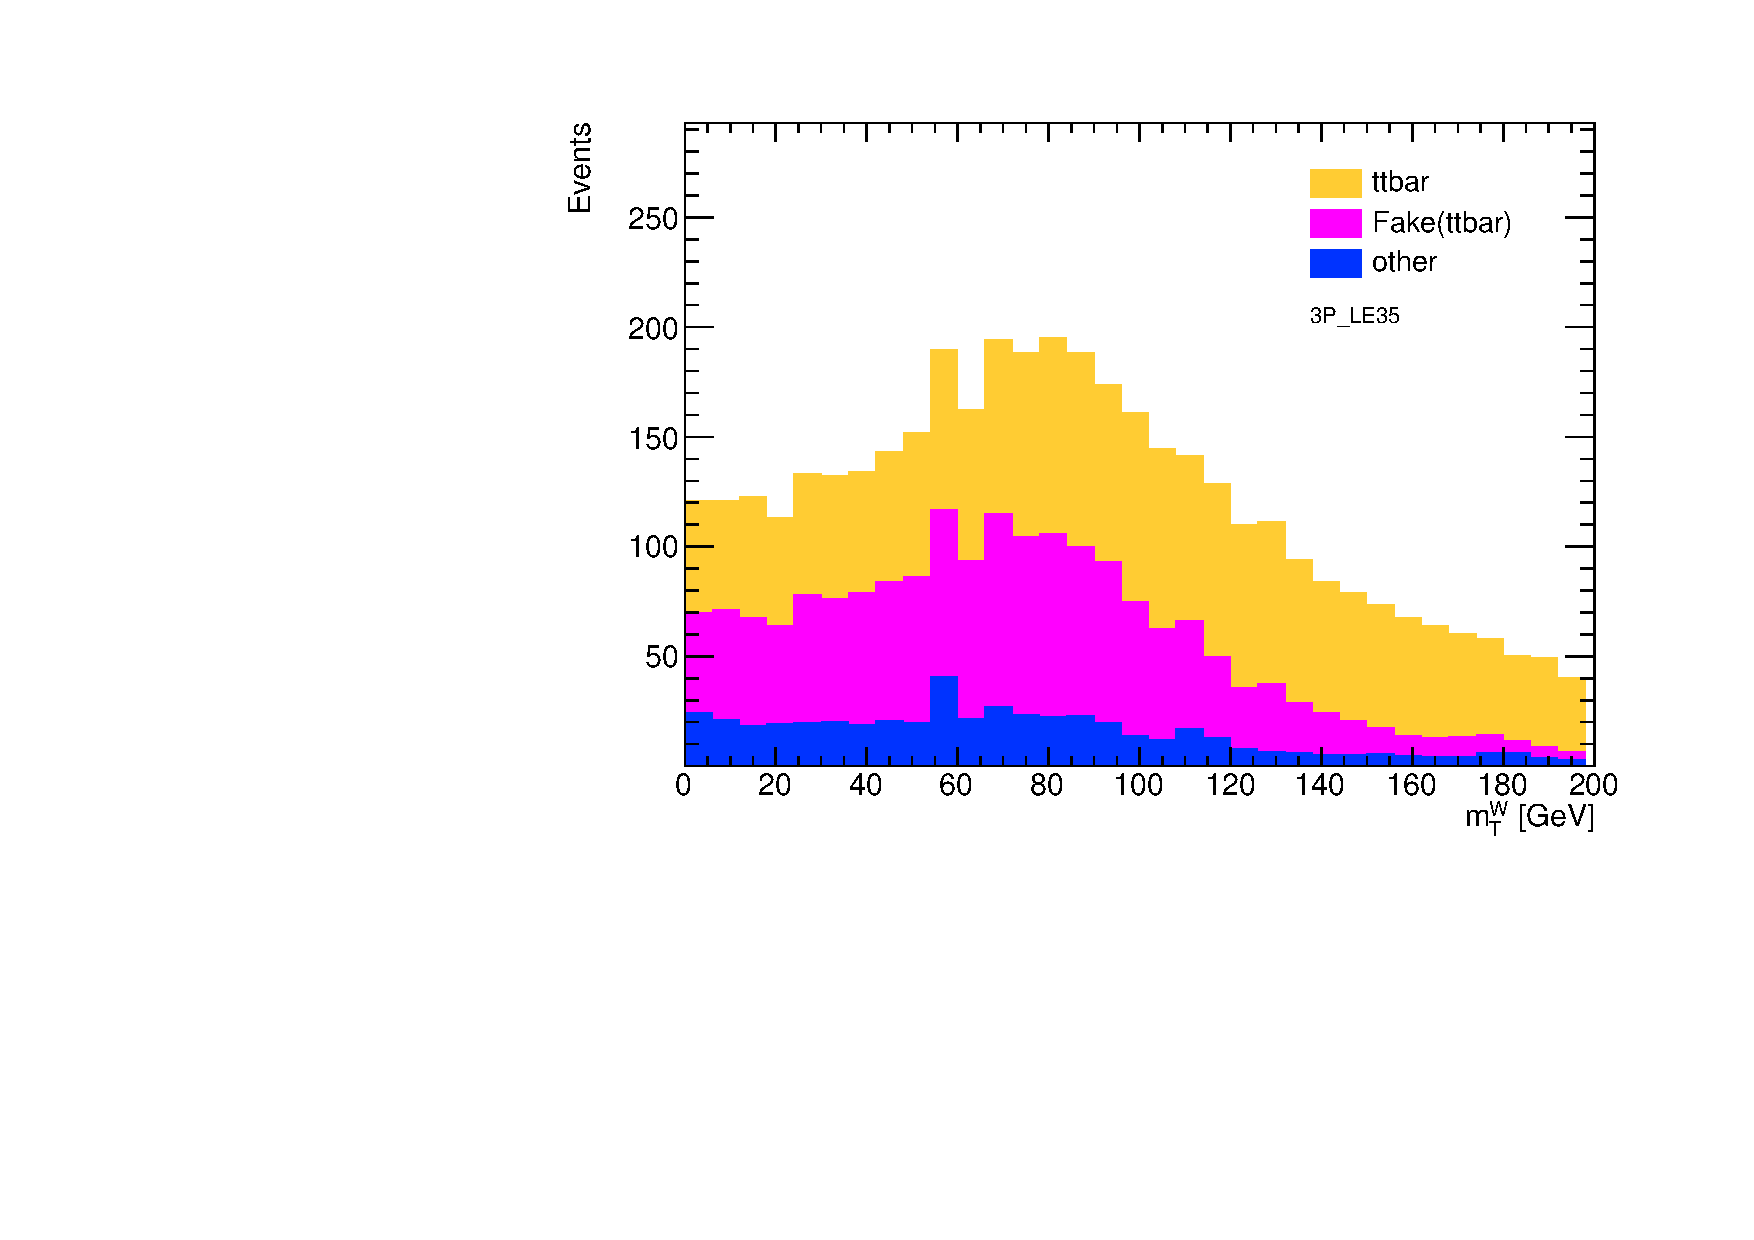
\includegraphics[scale=0.15]{mtw_fine_binning_stGE400LT500_3P_LE35}}
        \subfloat[$35<p_T<40$] {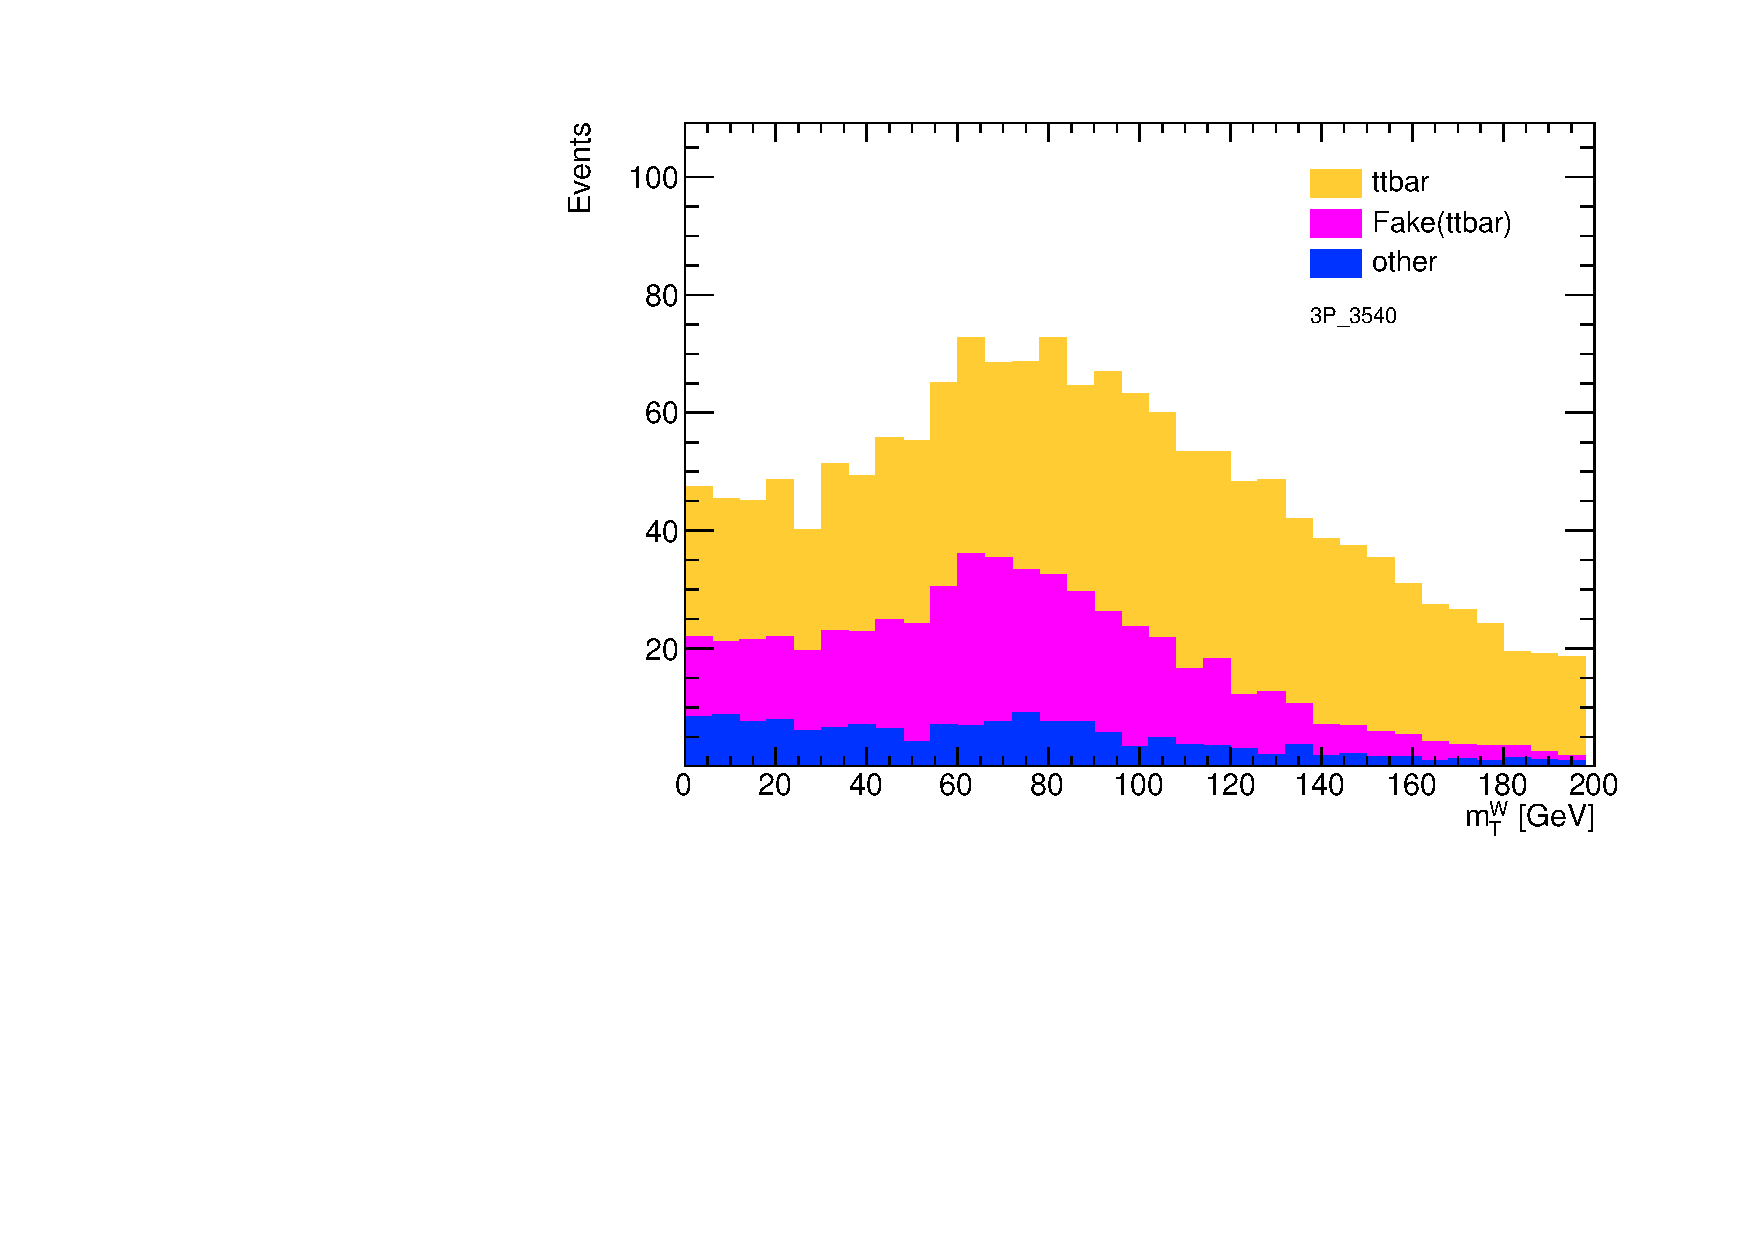
\includegraphics[scale=0.15]{mtw_fine_binning_stGE400LT500_3P_3540}}
        \subfloat[$40<p_T<45$] {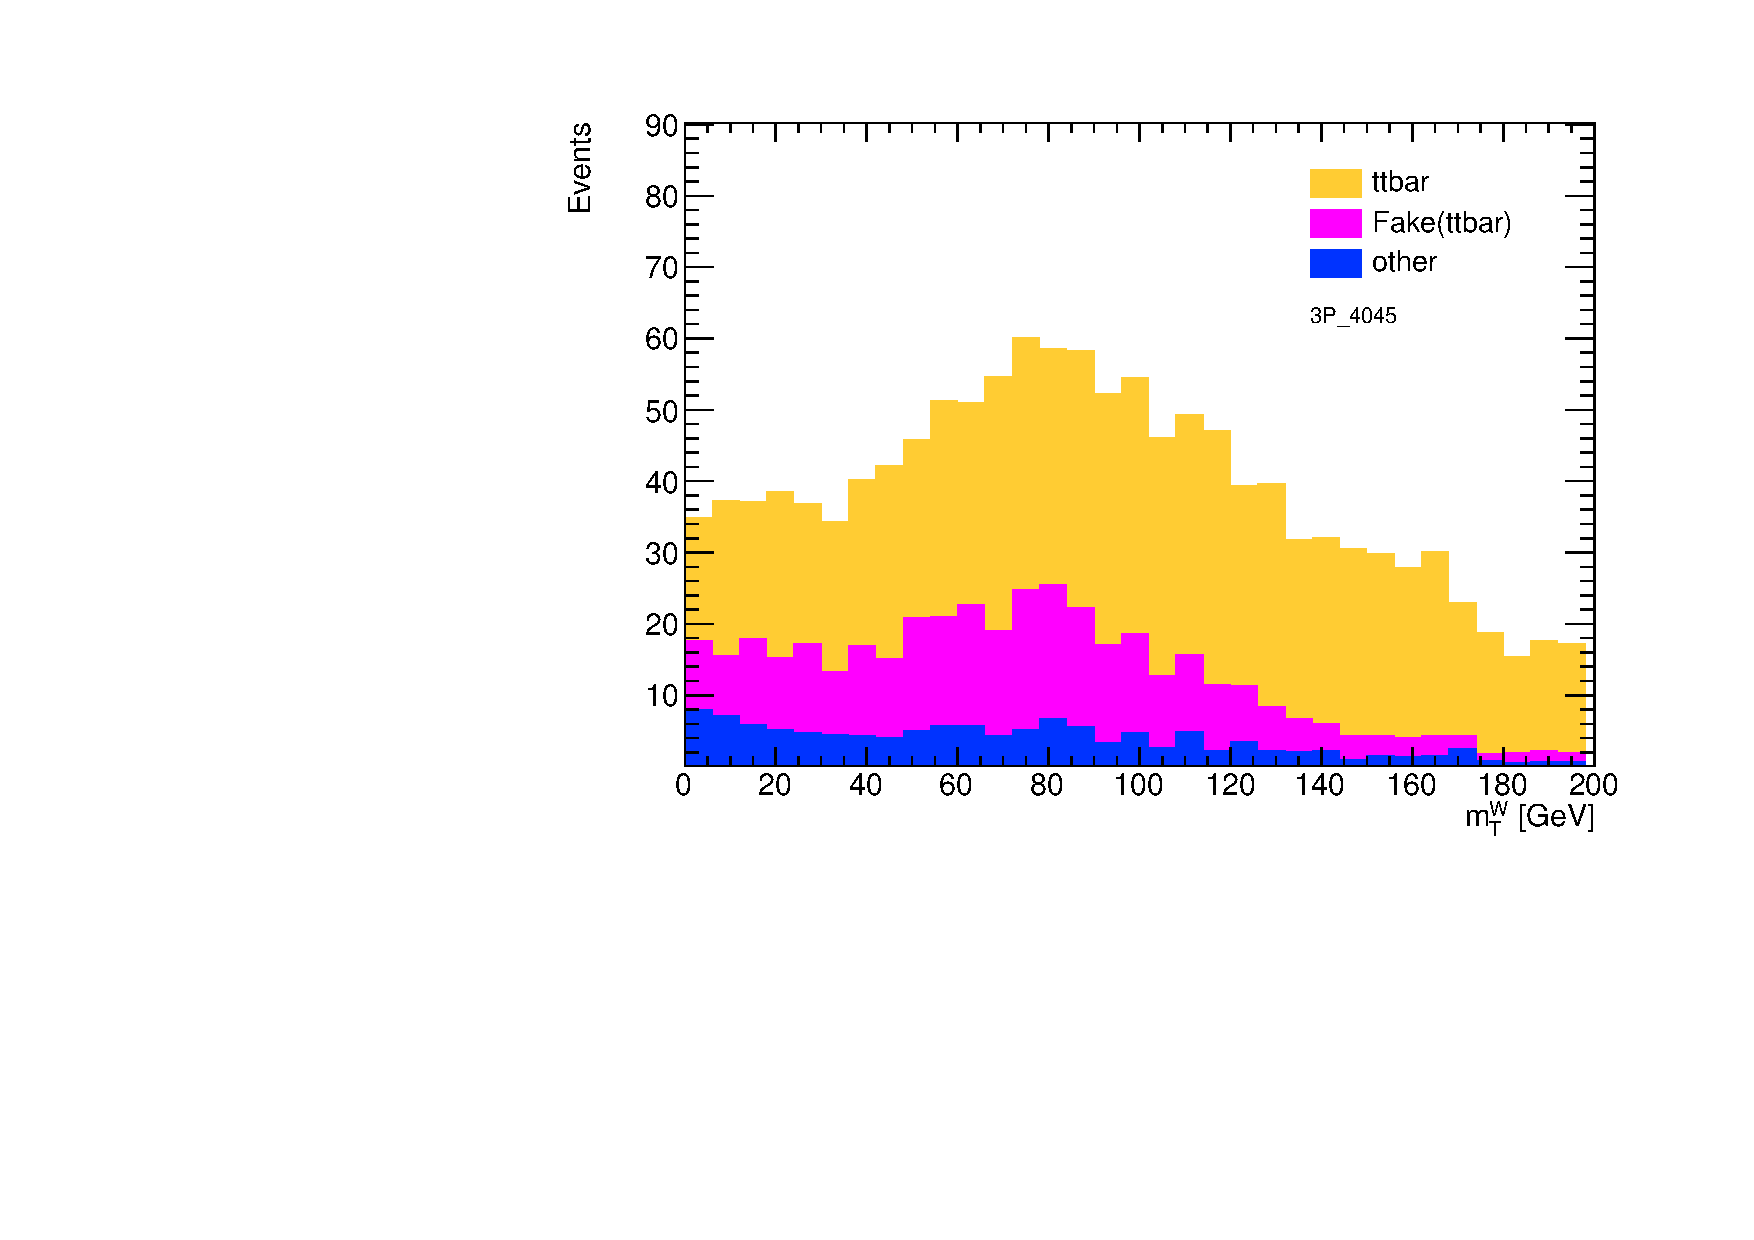
\includegraphics[scale=0.15]{mtw_fine_binning_stGE400LT500_3P_4045}}
        \subfloat[$45<p_T<50$] {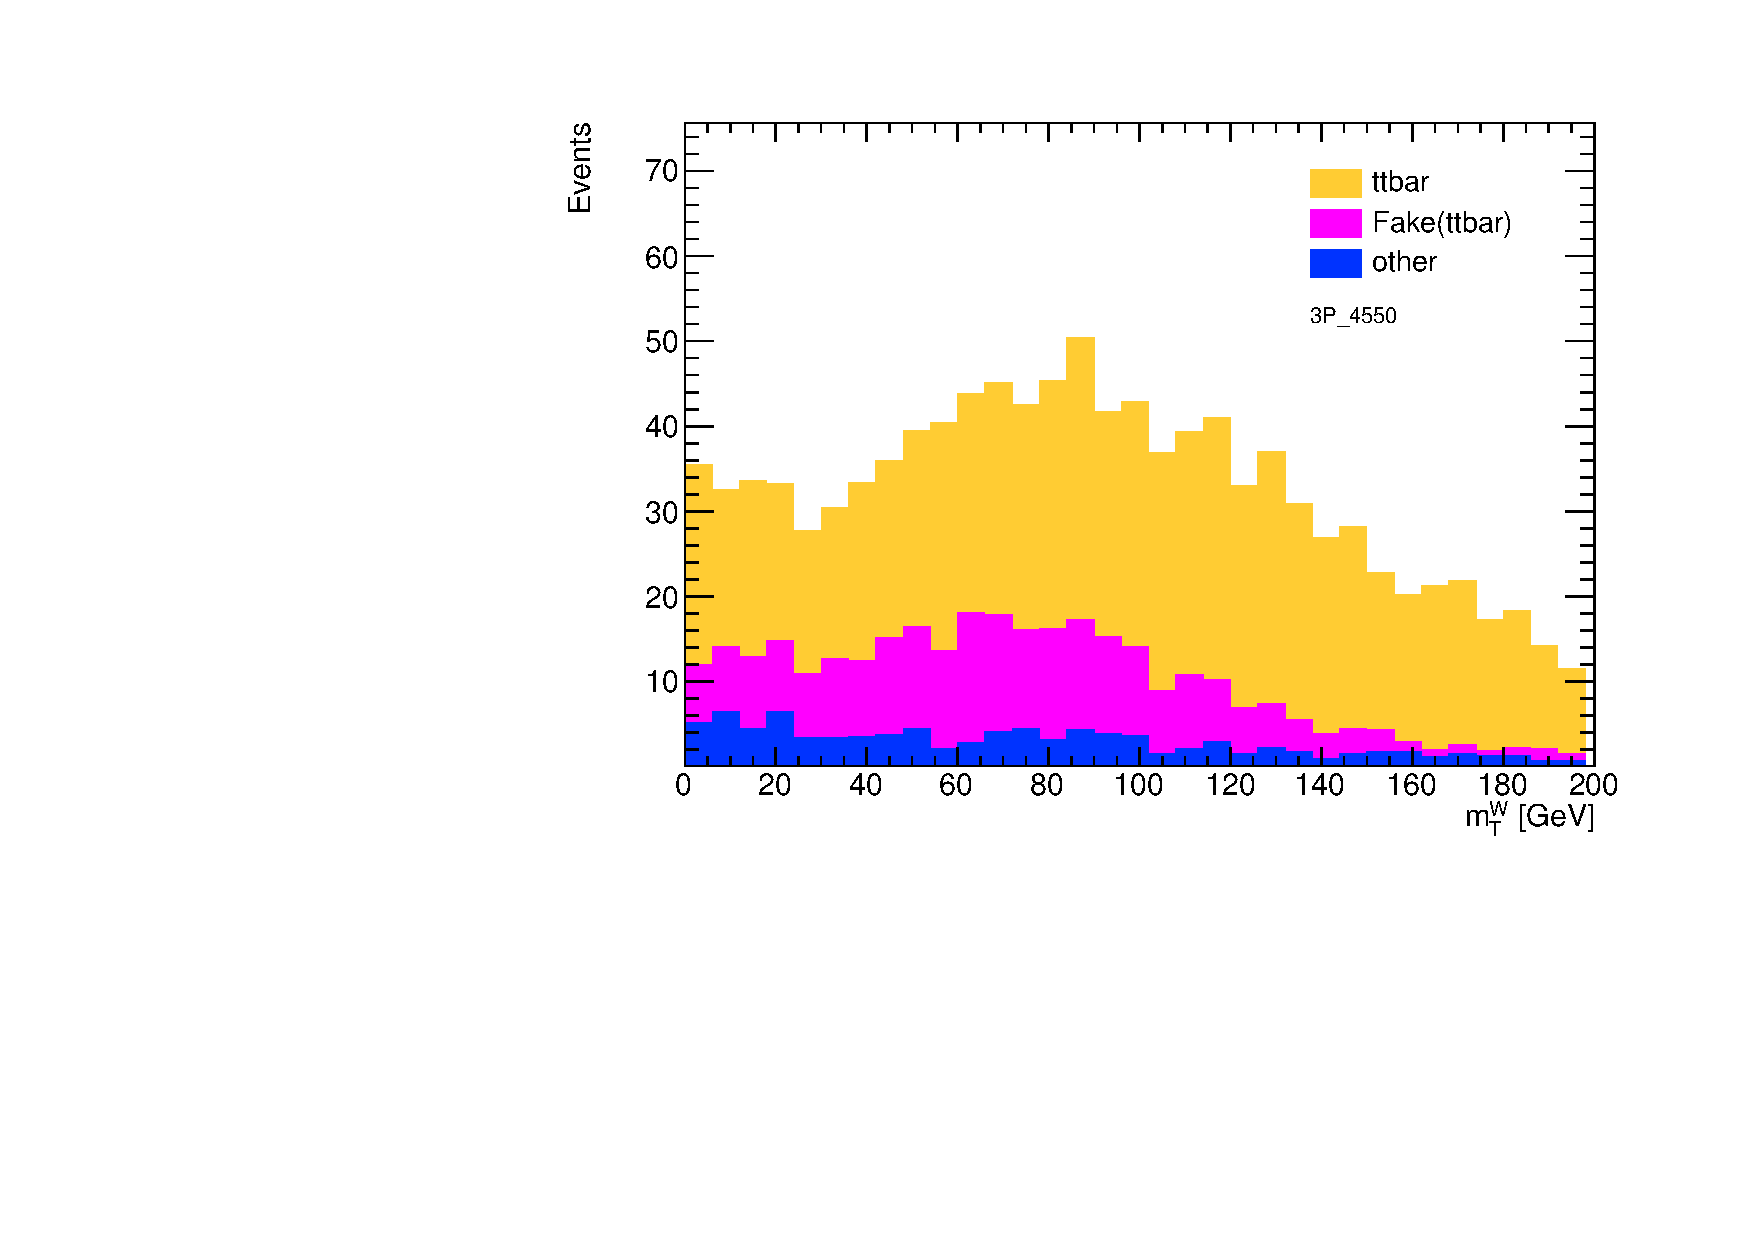
\includegraphics[scale=0.15]{mtw_fine_binning_stGE400LT500_3P_4550}} \\
        \subfloat[$50<p_T<55$] {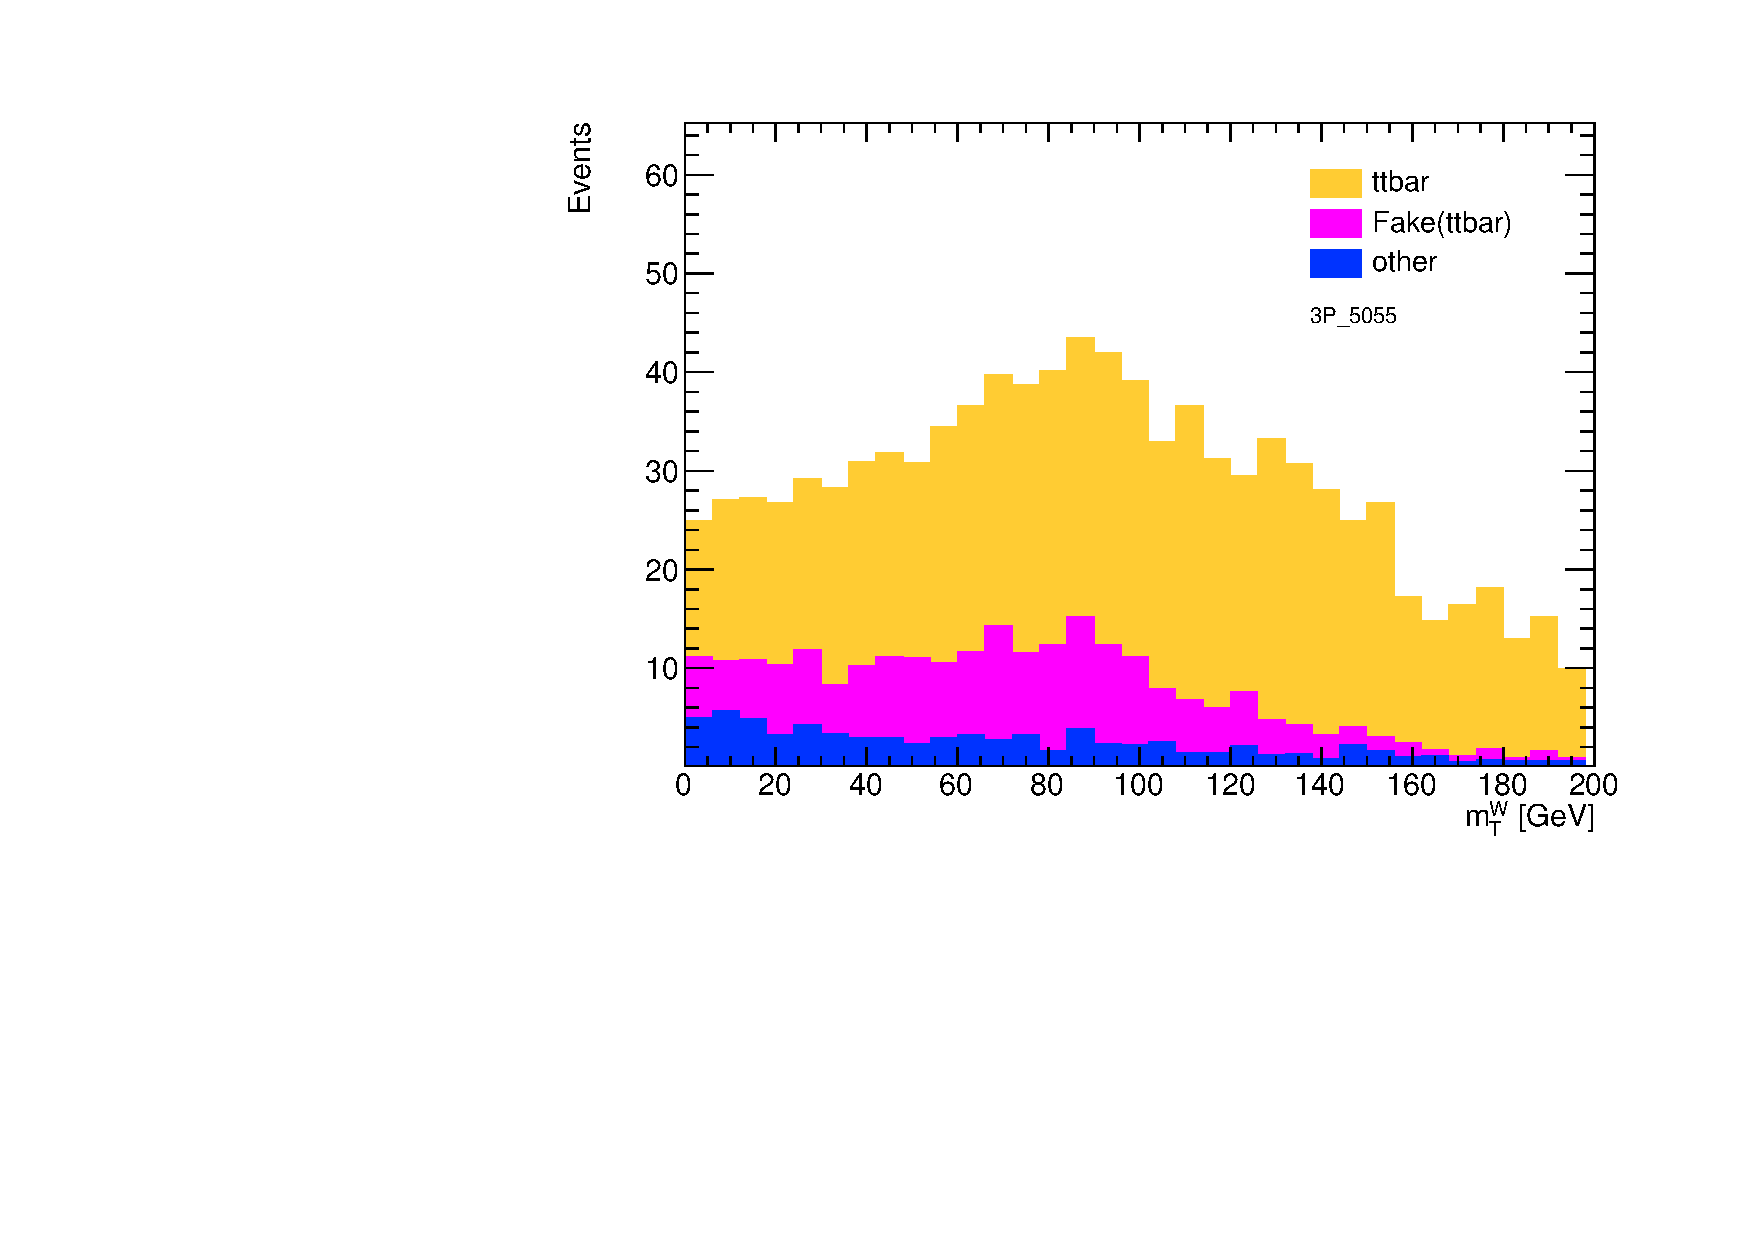
\includegraphics[scale=0.15]{mtw_fine_binning_stGE400LT500_3P_5055}}
        \subfloat[$55<p_T<70$] {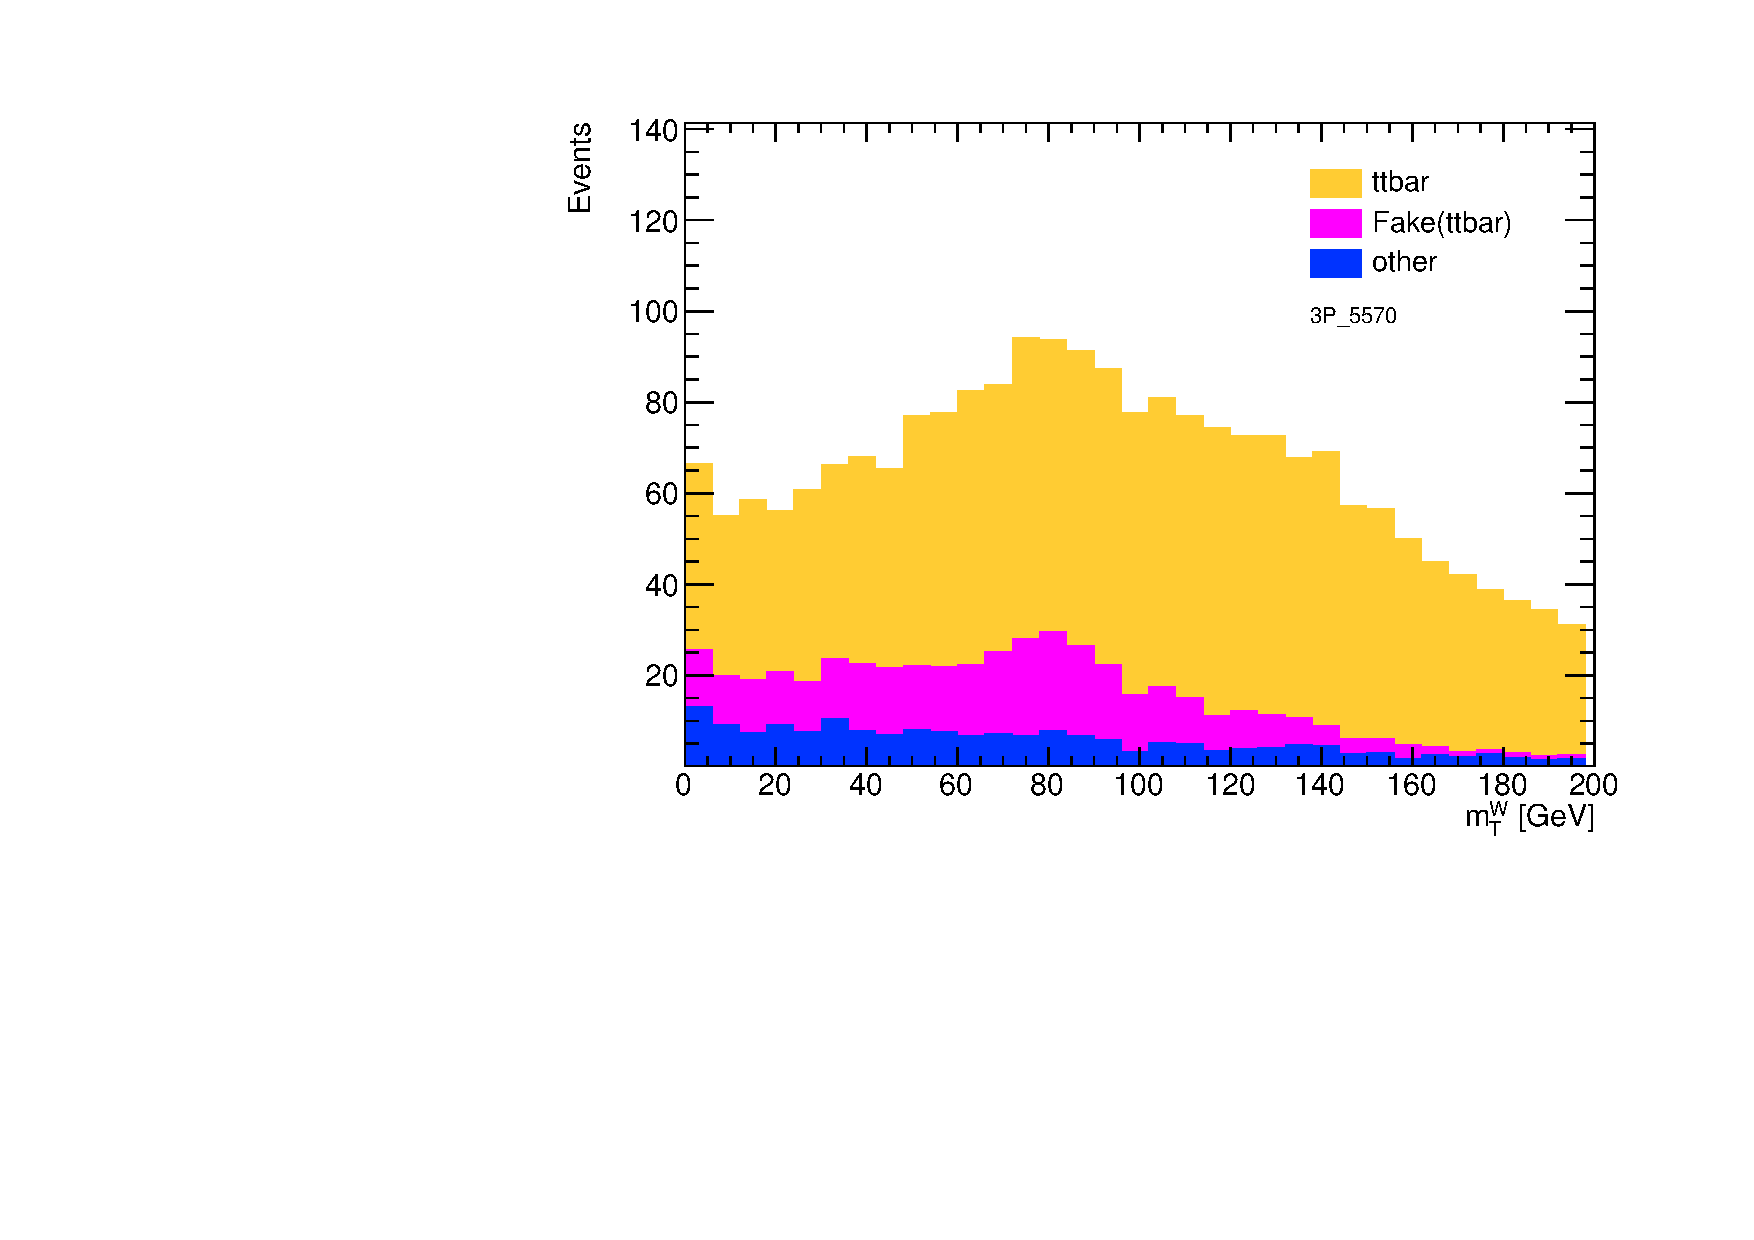
\includegraphics[scale=0.15]{mtw_fine_binning_stGE400LT500_3P_5570}}
        \subfloat[$70<p_T$]    {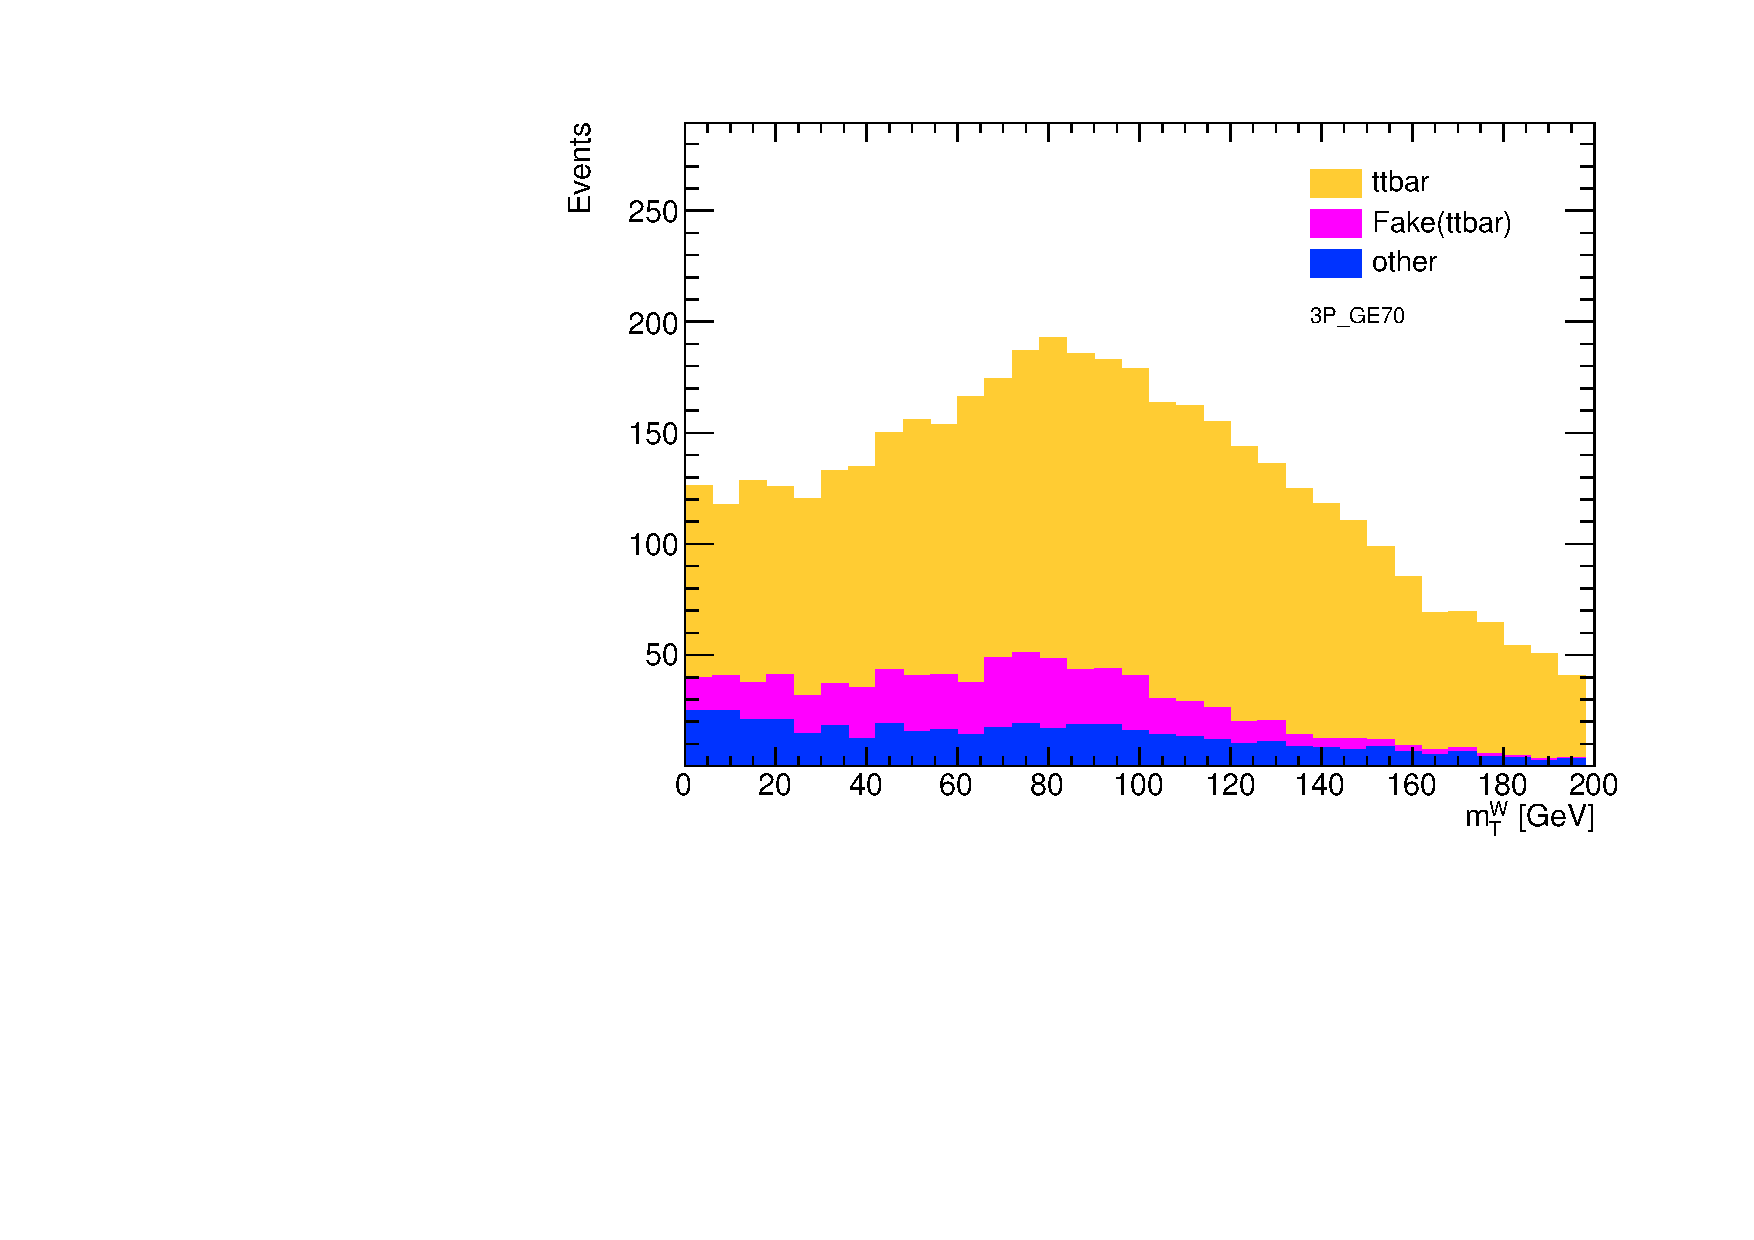
\includegraphics[scale=0.15]{mtw_fine_binning_stGE400LT500_3P_GE70}}
  \end{figure}       
\end{frame}

\begin{frame}{\mtw distribution (1-prong, CR3)}
  \begin{figure}
    \setcounter{subfigure}{0}
    \centering
        \subfloat[$p_T<35$]    {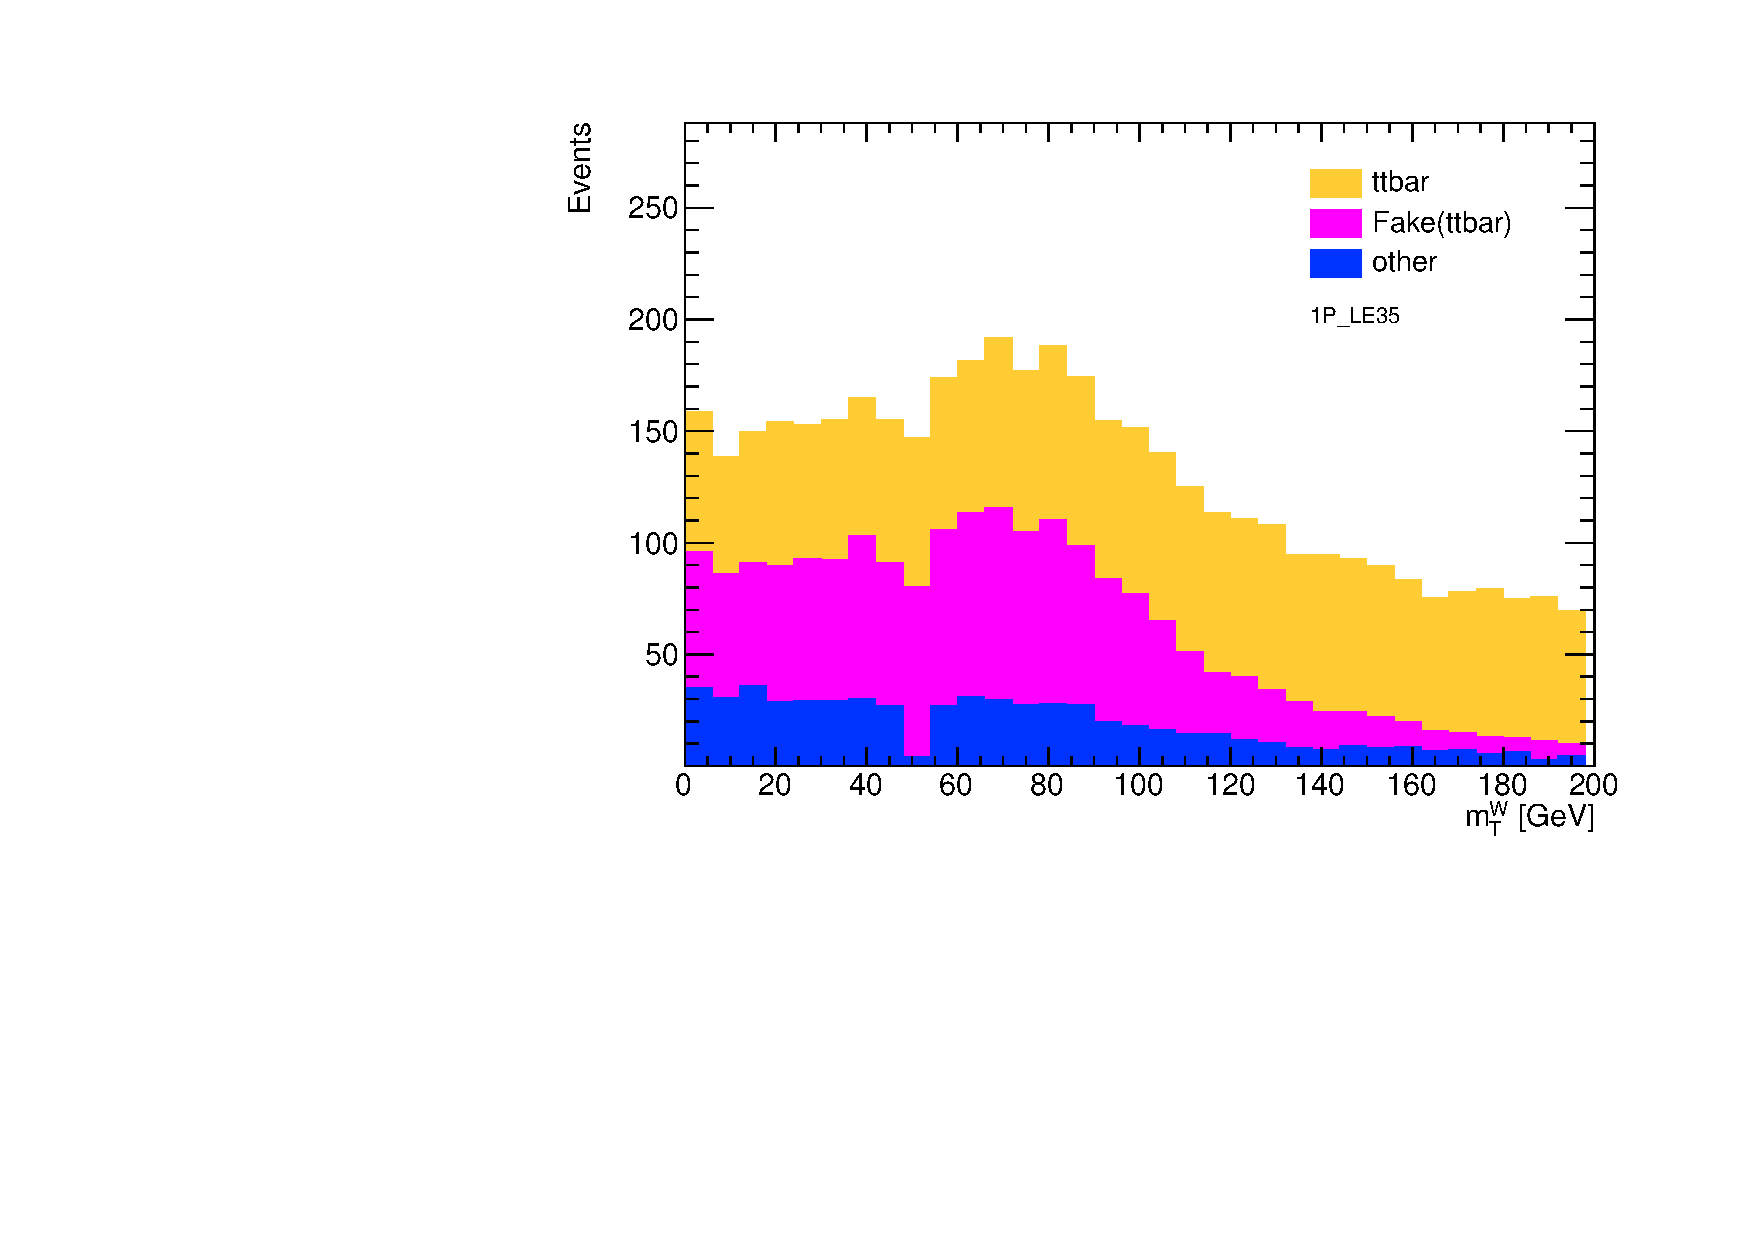
\includegraphics[scale=0.15]{mtw_fine_binning_stGE500LT600_1P_LE35}}
        \subfloat[$35<p_T<40$] {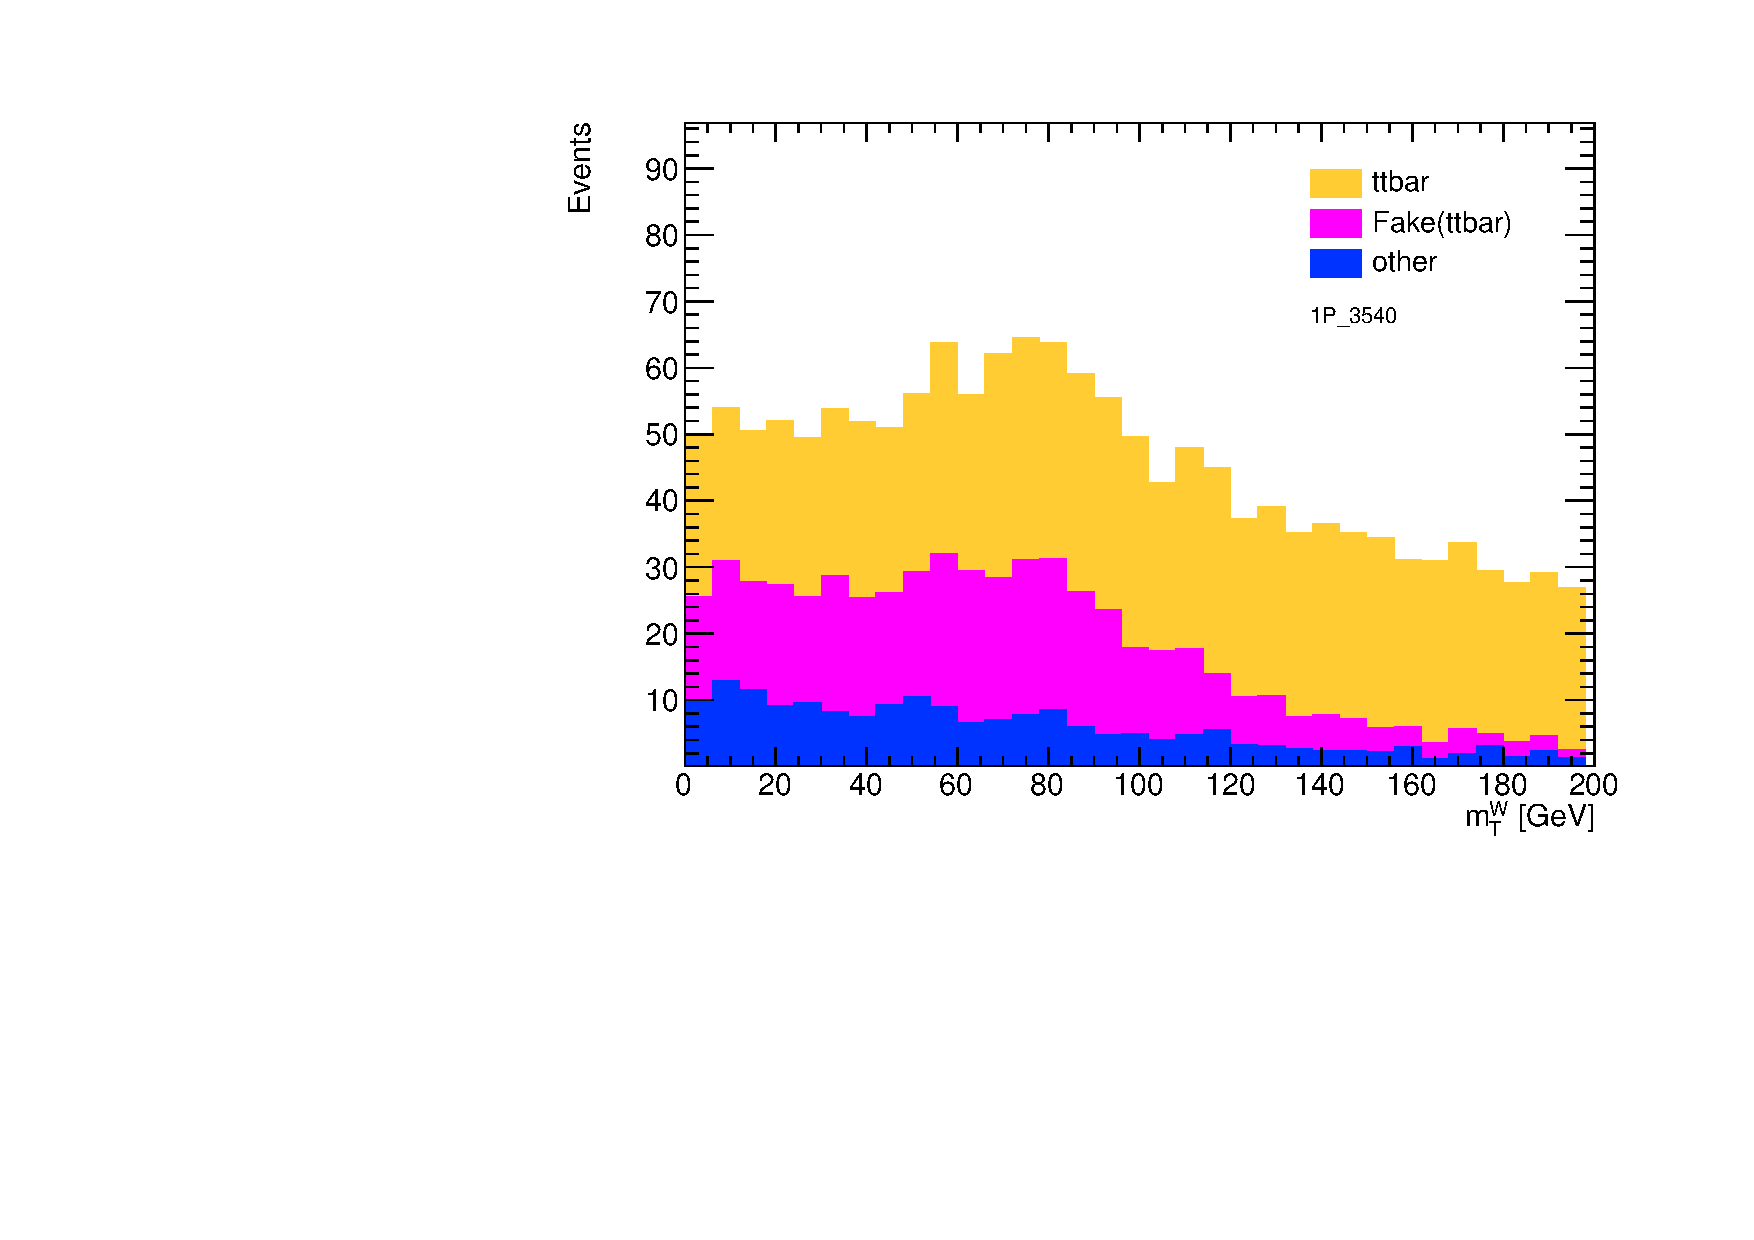
\includegraphics[scale=0.15]{mtw_fine_binning_stGE500LT600_1P_3540}}
        \subfloat[$40<p_T<45$] {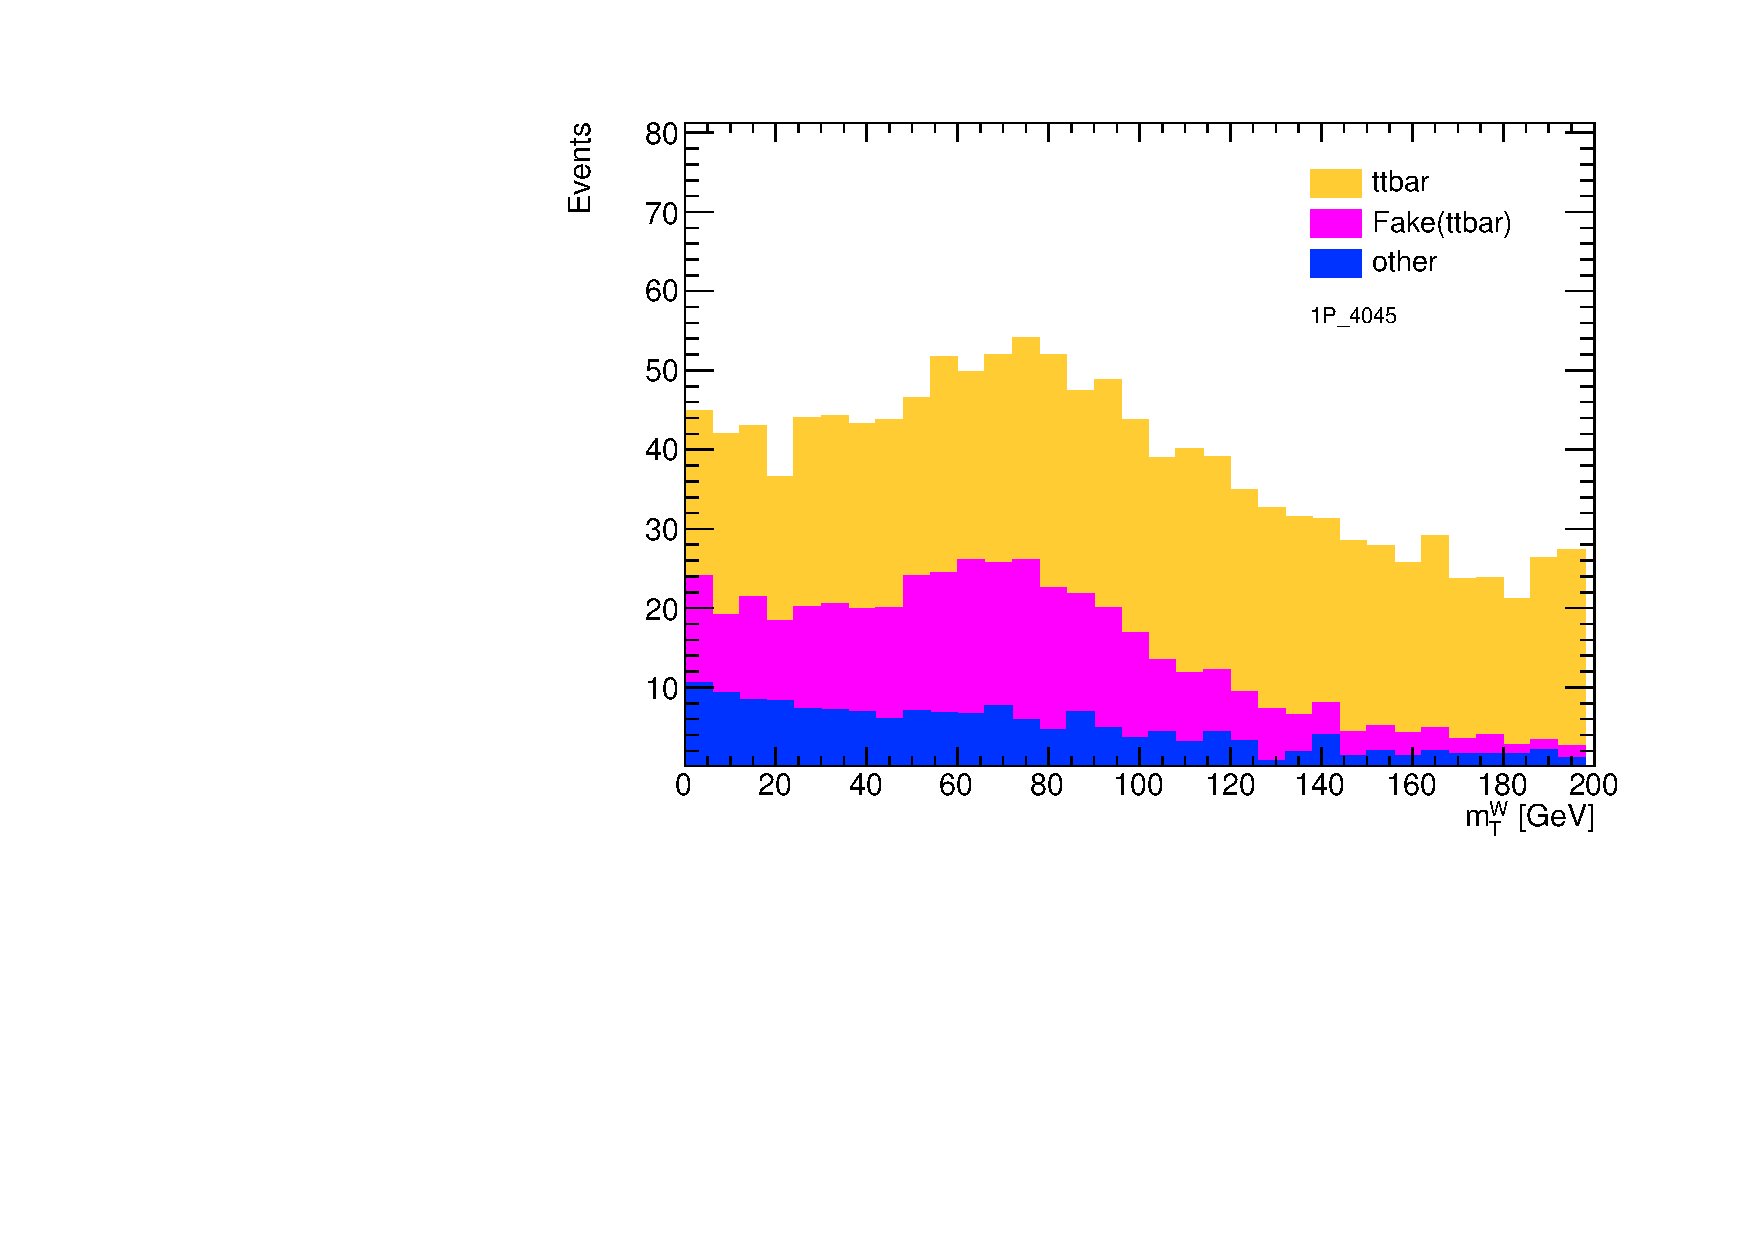
\includegraphics[scale=0.15]{mtw_fine_binning_stGE500LT600_1P_4045}}
        \subfloat[$45<p_T<50$] {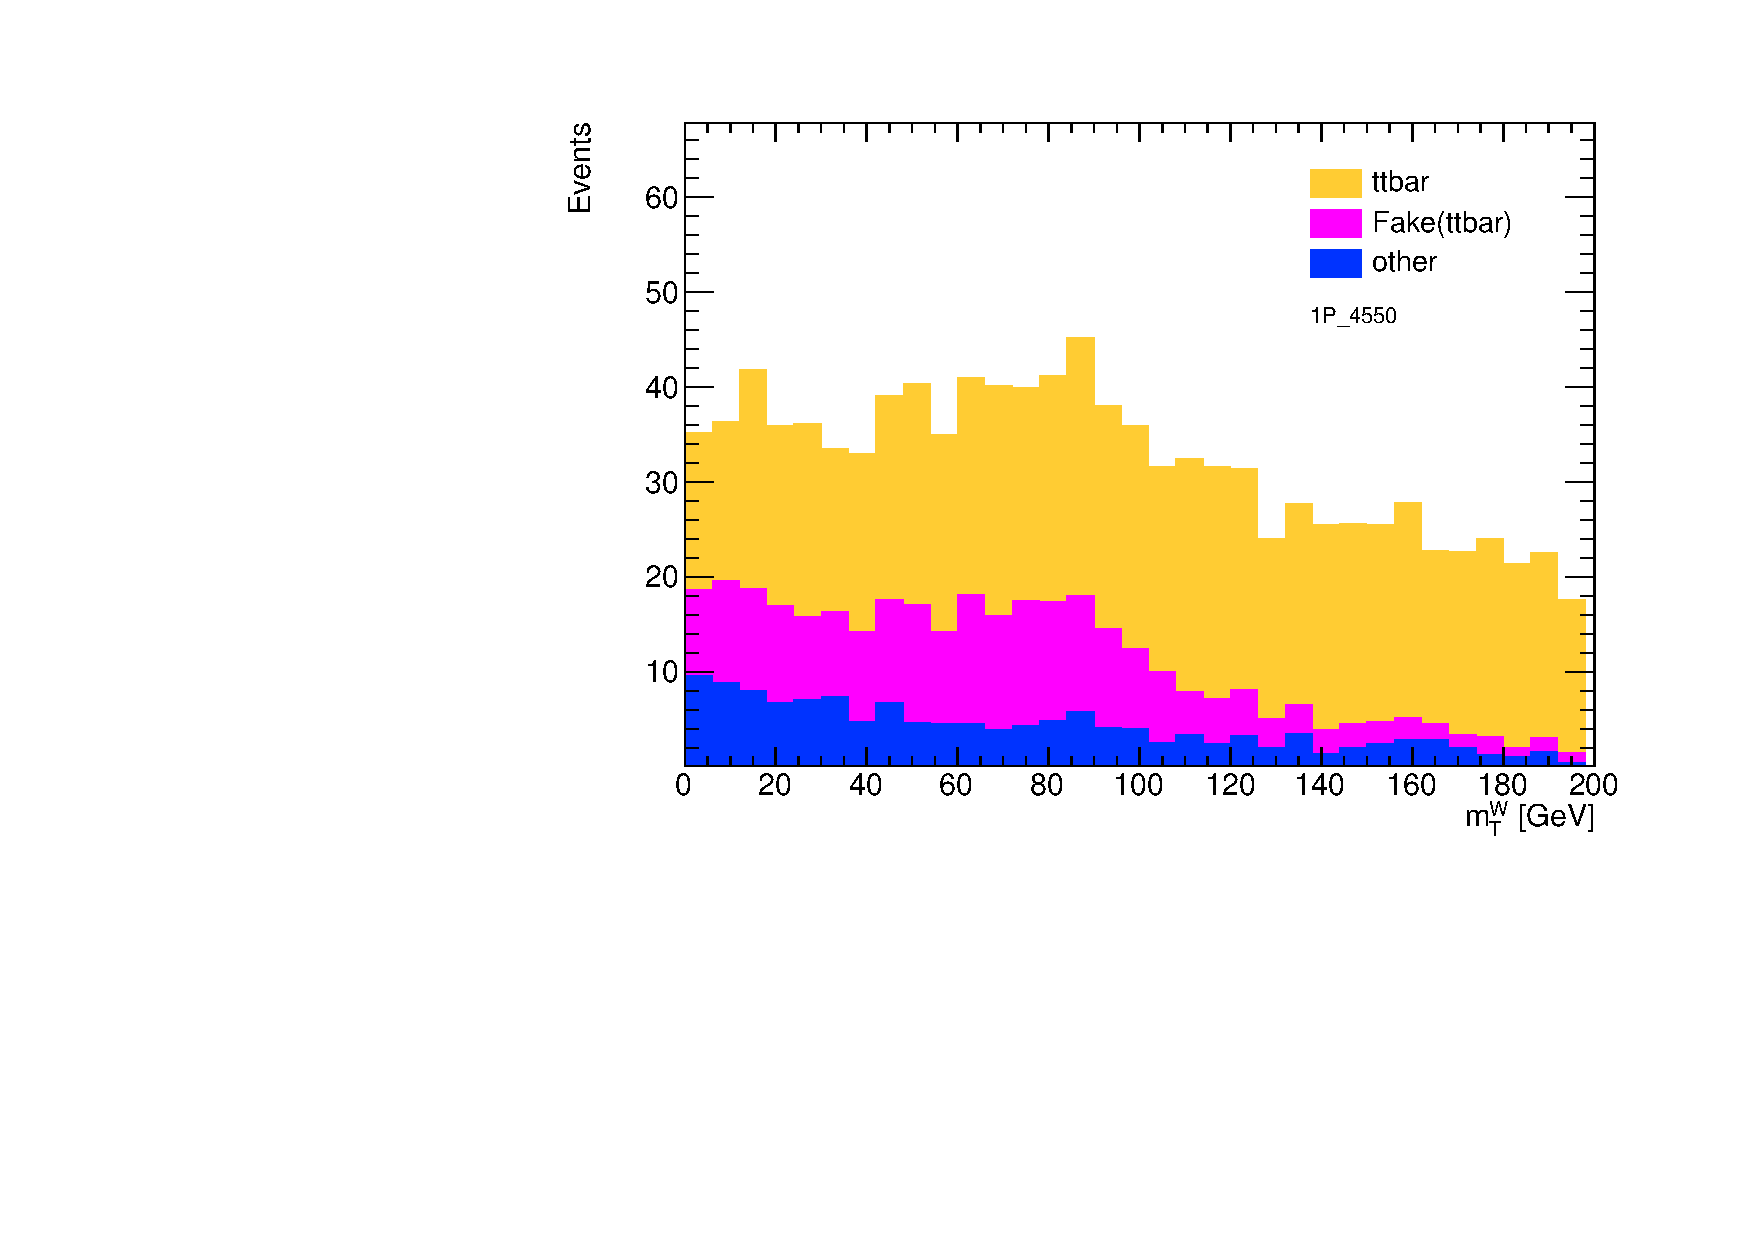
\includegraphics[scale=0.15]{mtw_fine_binning_stGE500LT600_1P_4550}} \\
        \subfloat[$50<p_T<55$] {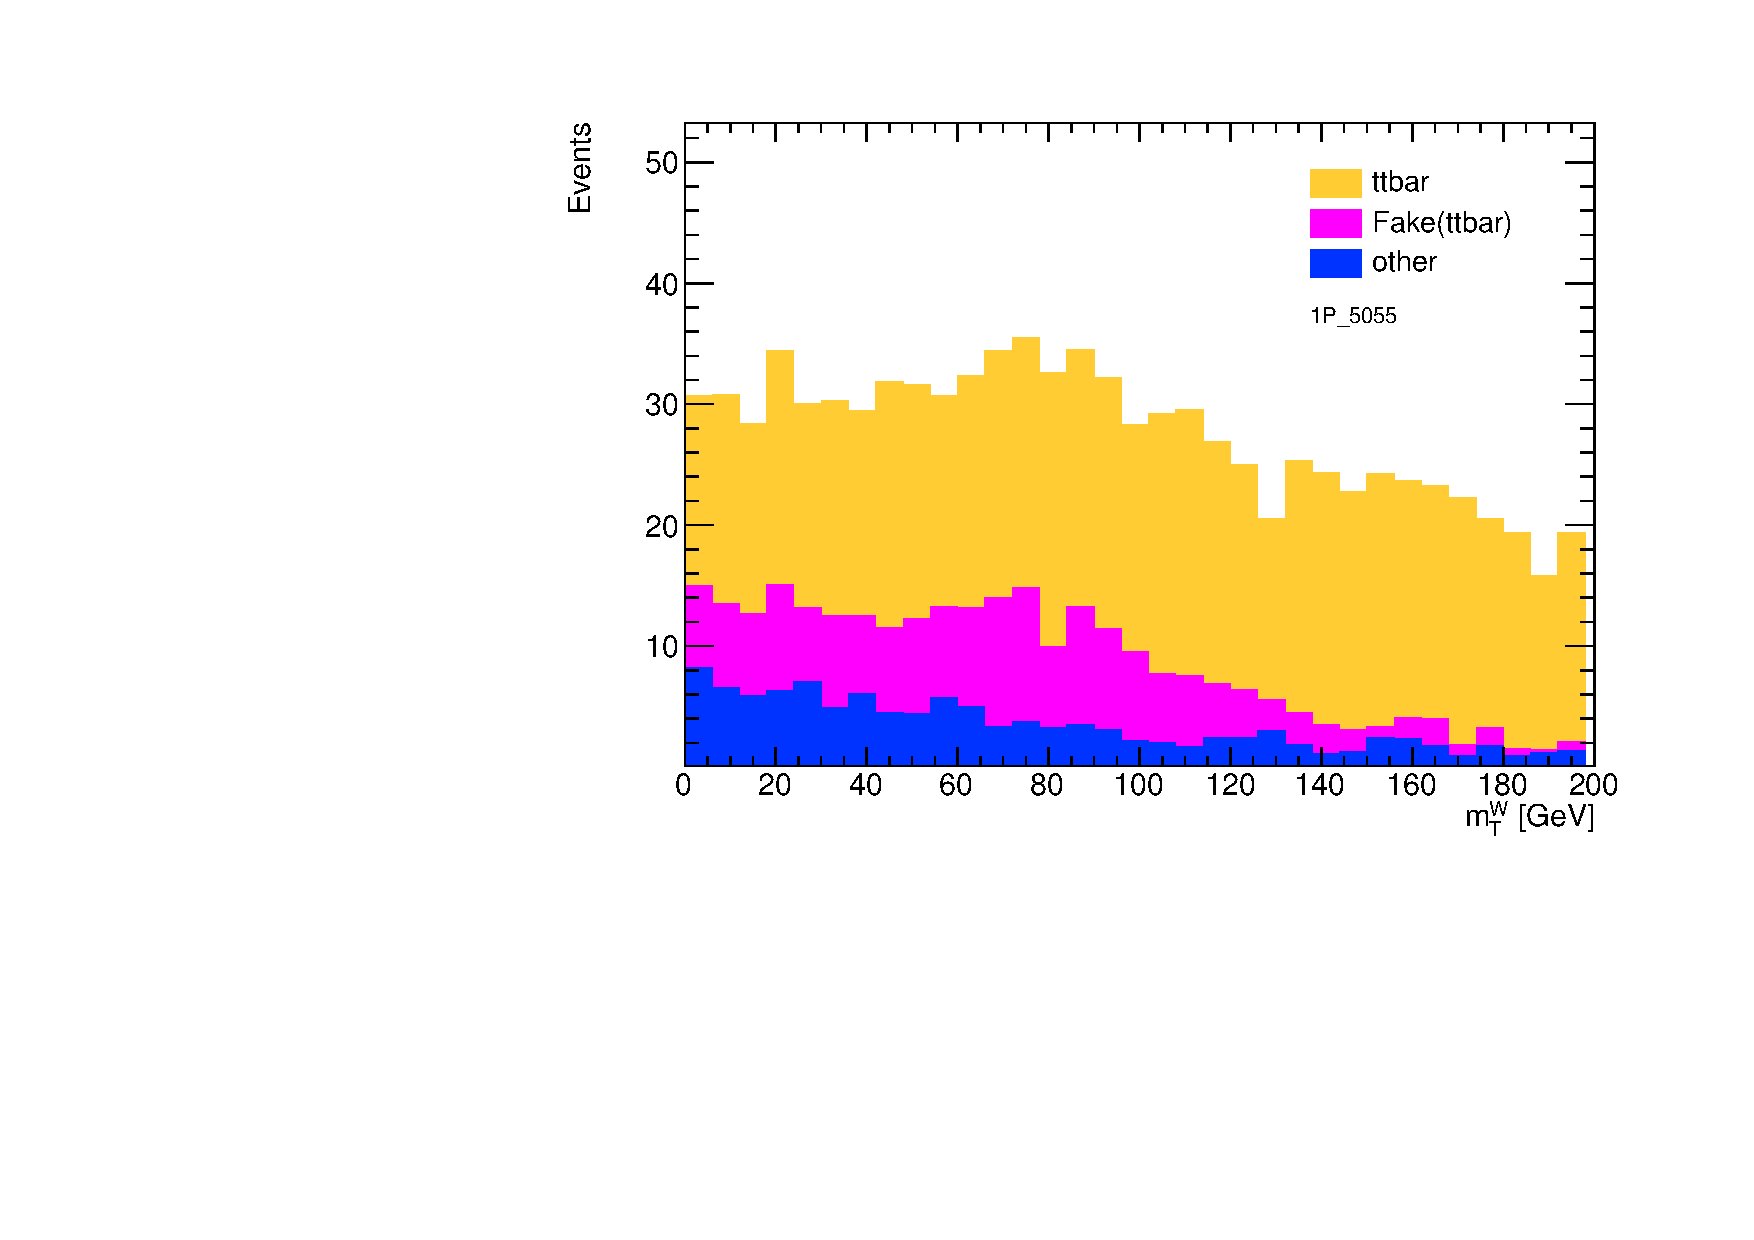
\includegraphics[scale=0.15]{mtw_fine_binning_stGE500LT600_1P_5055}}
        \subfloat[$55<p_T<70$] {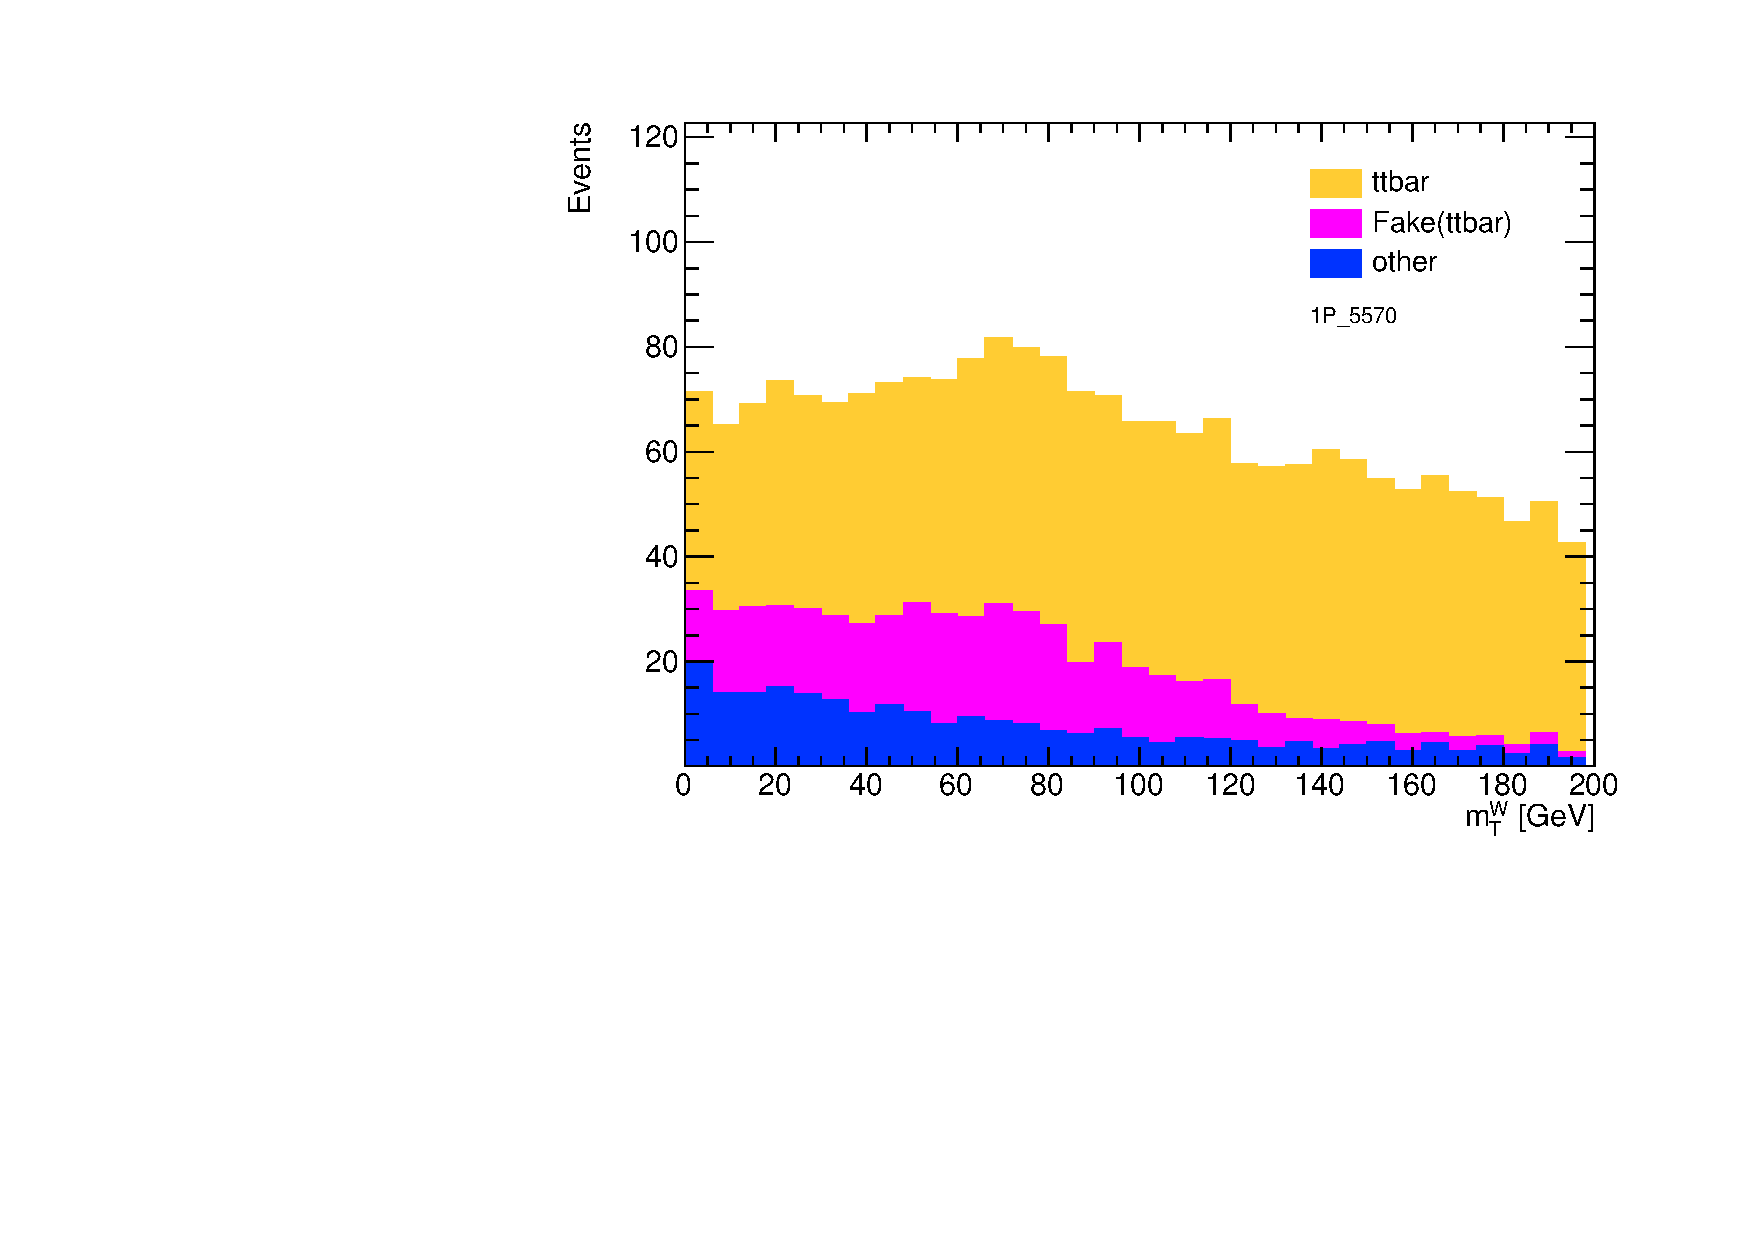
\includegraphics[scale=0.15]{mtw_fine_binning_stGE500LT600_1P_5570}}
        \subfloat[$70<p_T<100$]{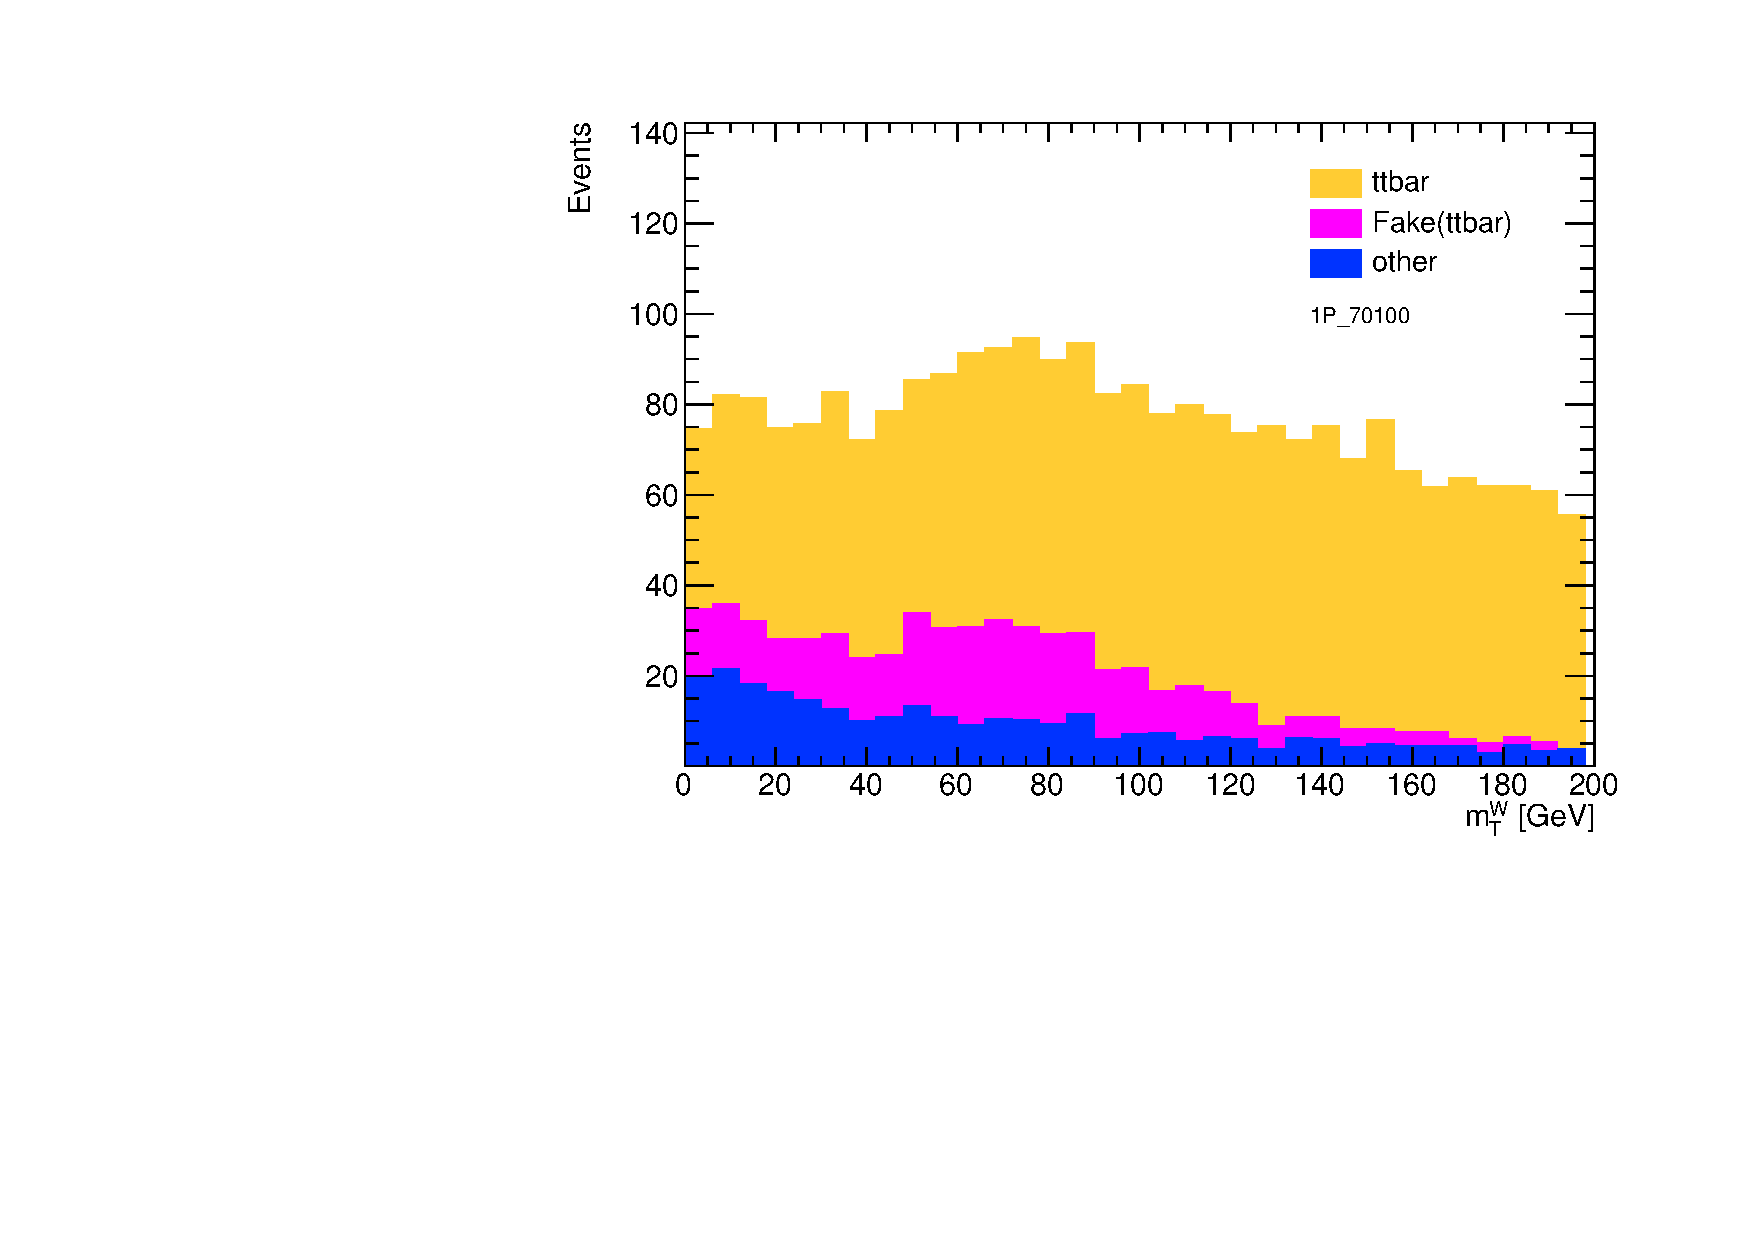
\includegraphics[scale=0.15]{mtw_fine_binning_stGE500LT600_1P_70100}}
        \subfloat[$100<p_T$]   {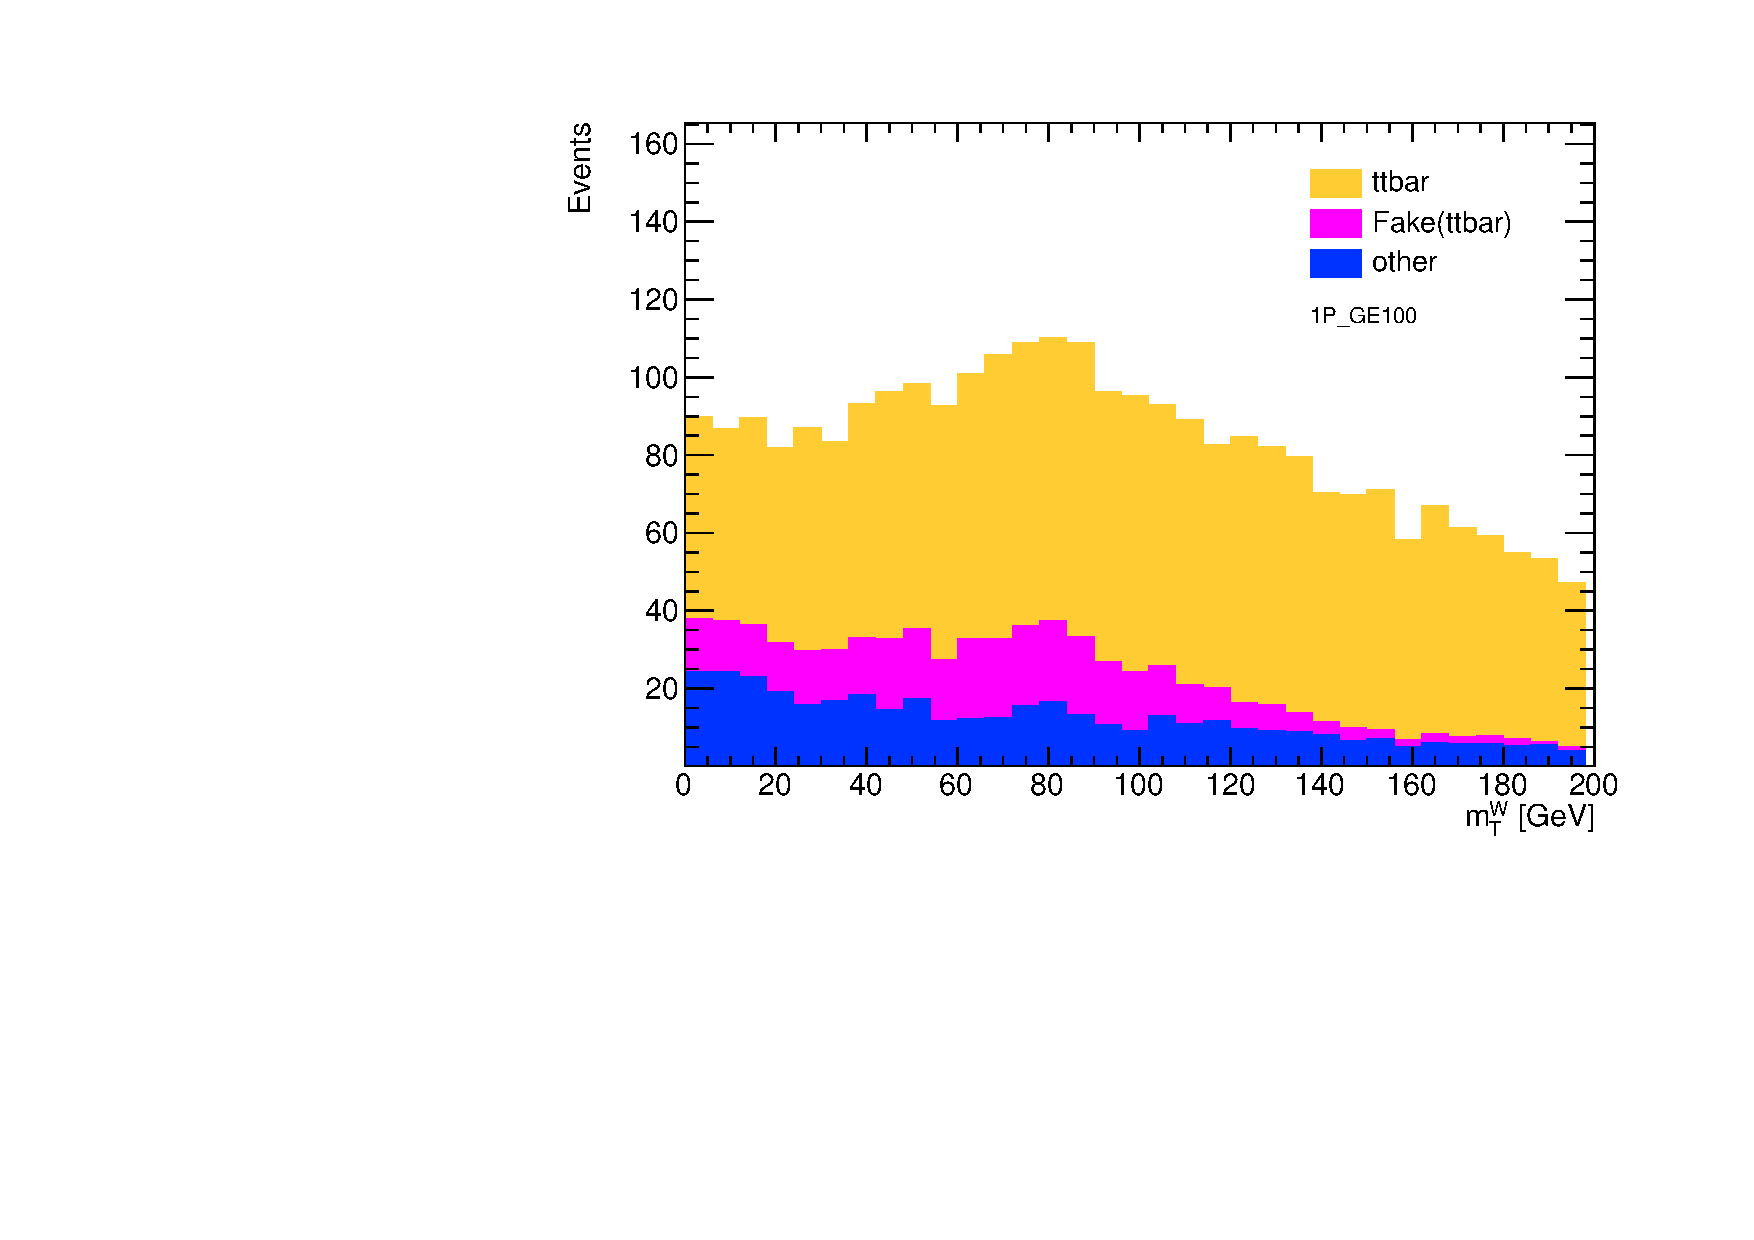
\includegraphics[scale=0.15]{mtw_fine_binning_stGE500LT600_1P_GE100}}\\
  \end{figure}
\end{frame}

\begin{frame}{\mtw distribution (3-prong, CR3)}
  \begin{figure}
    \setcounter{subfigure}{0}
    \centering
        \subfloat[$p_T<35$]    {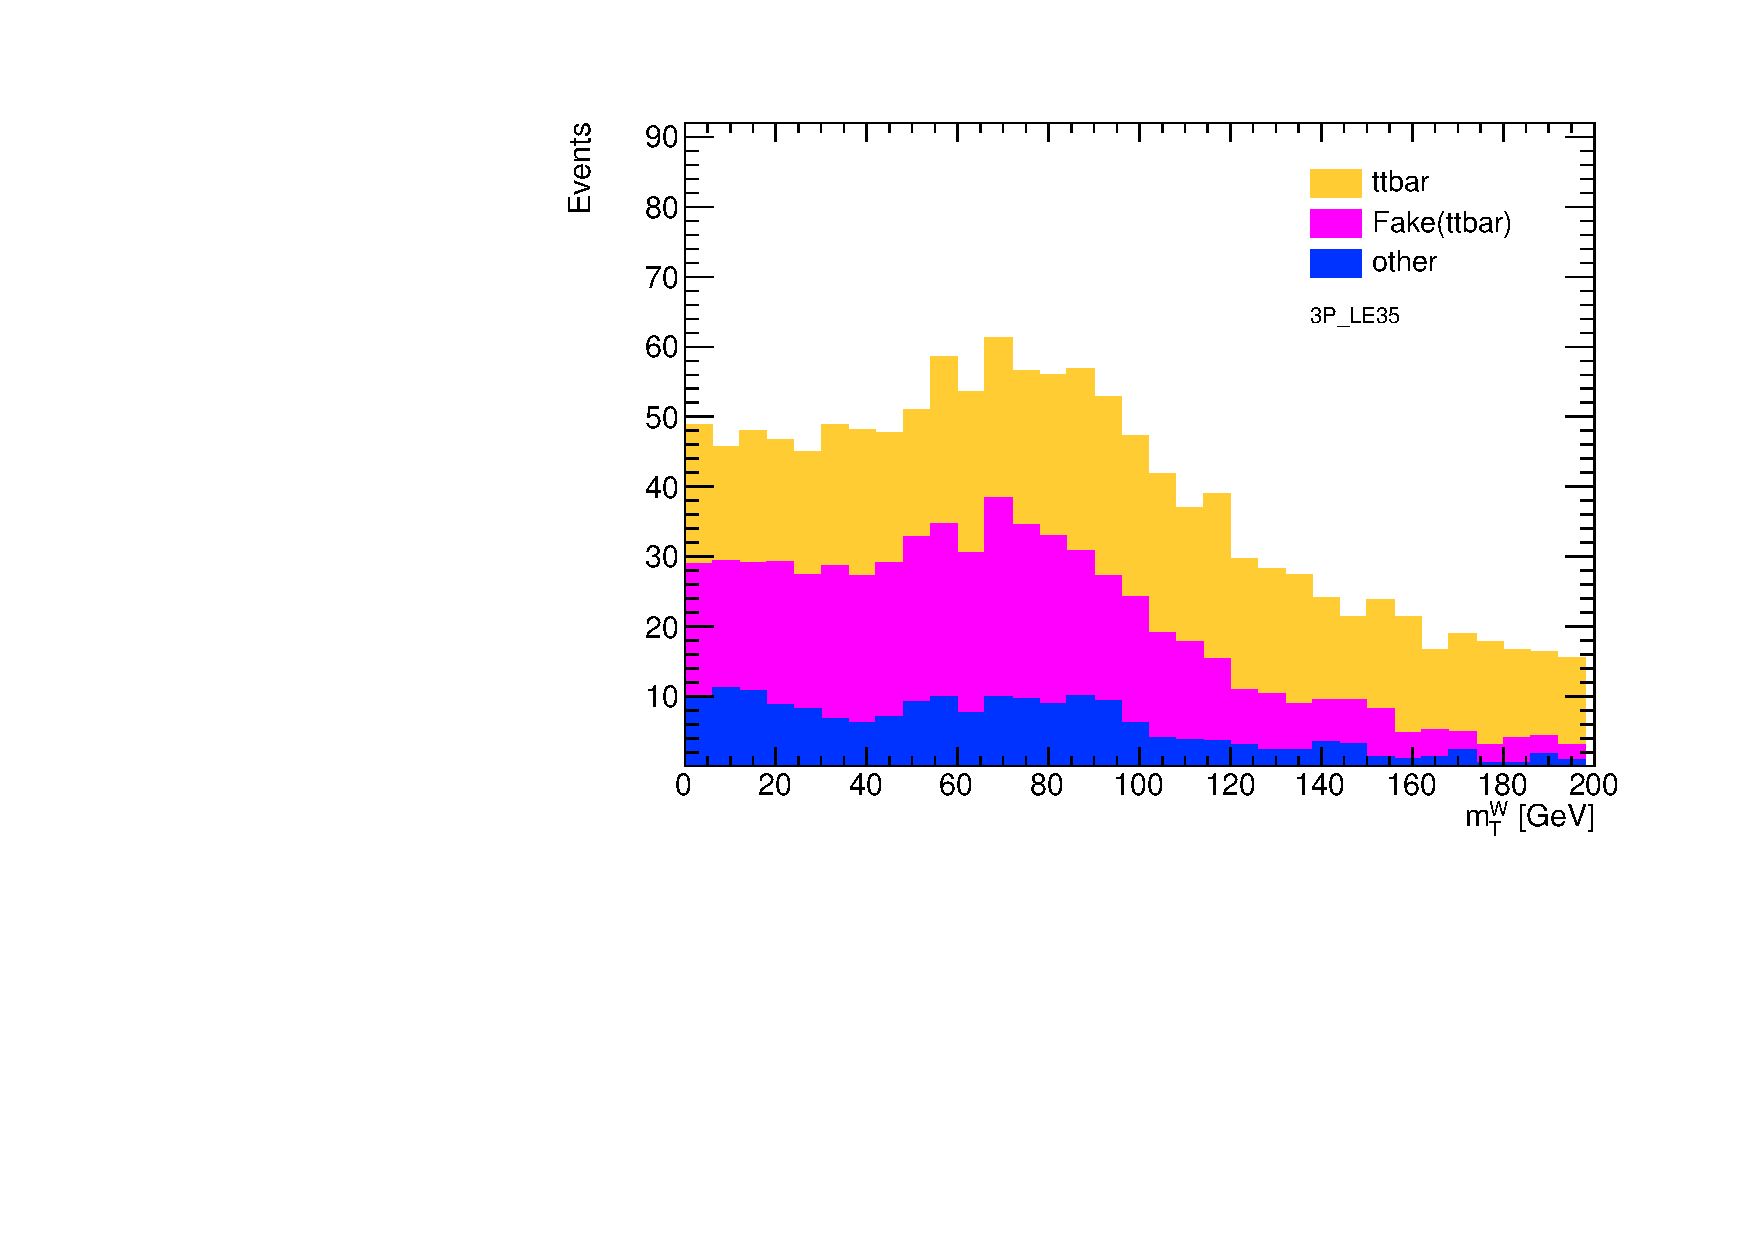
\includegraphics[scale=0.15]{mtw_fine_binning_stGE500LT600_3P_LE35}}
        \subfloat[$35<p_T<40$] {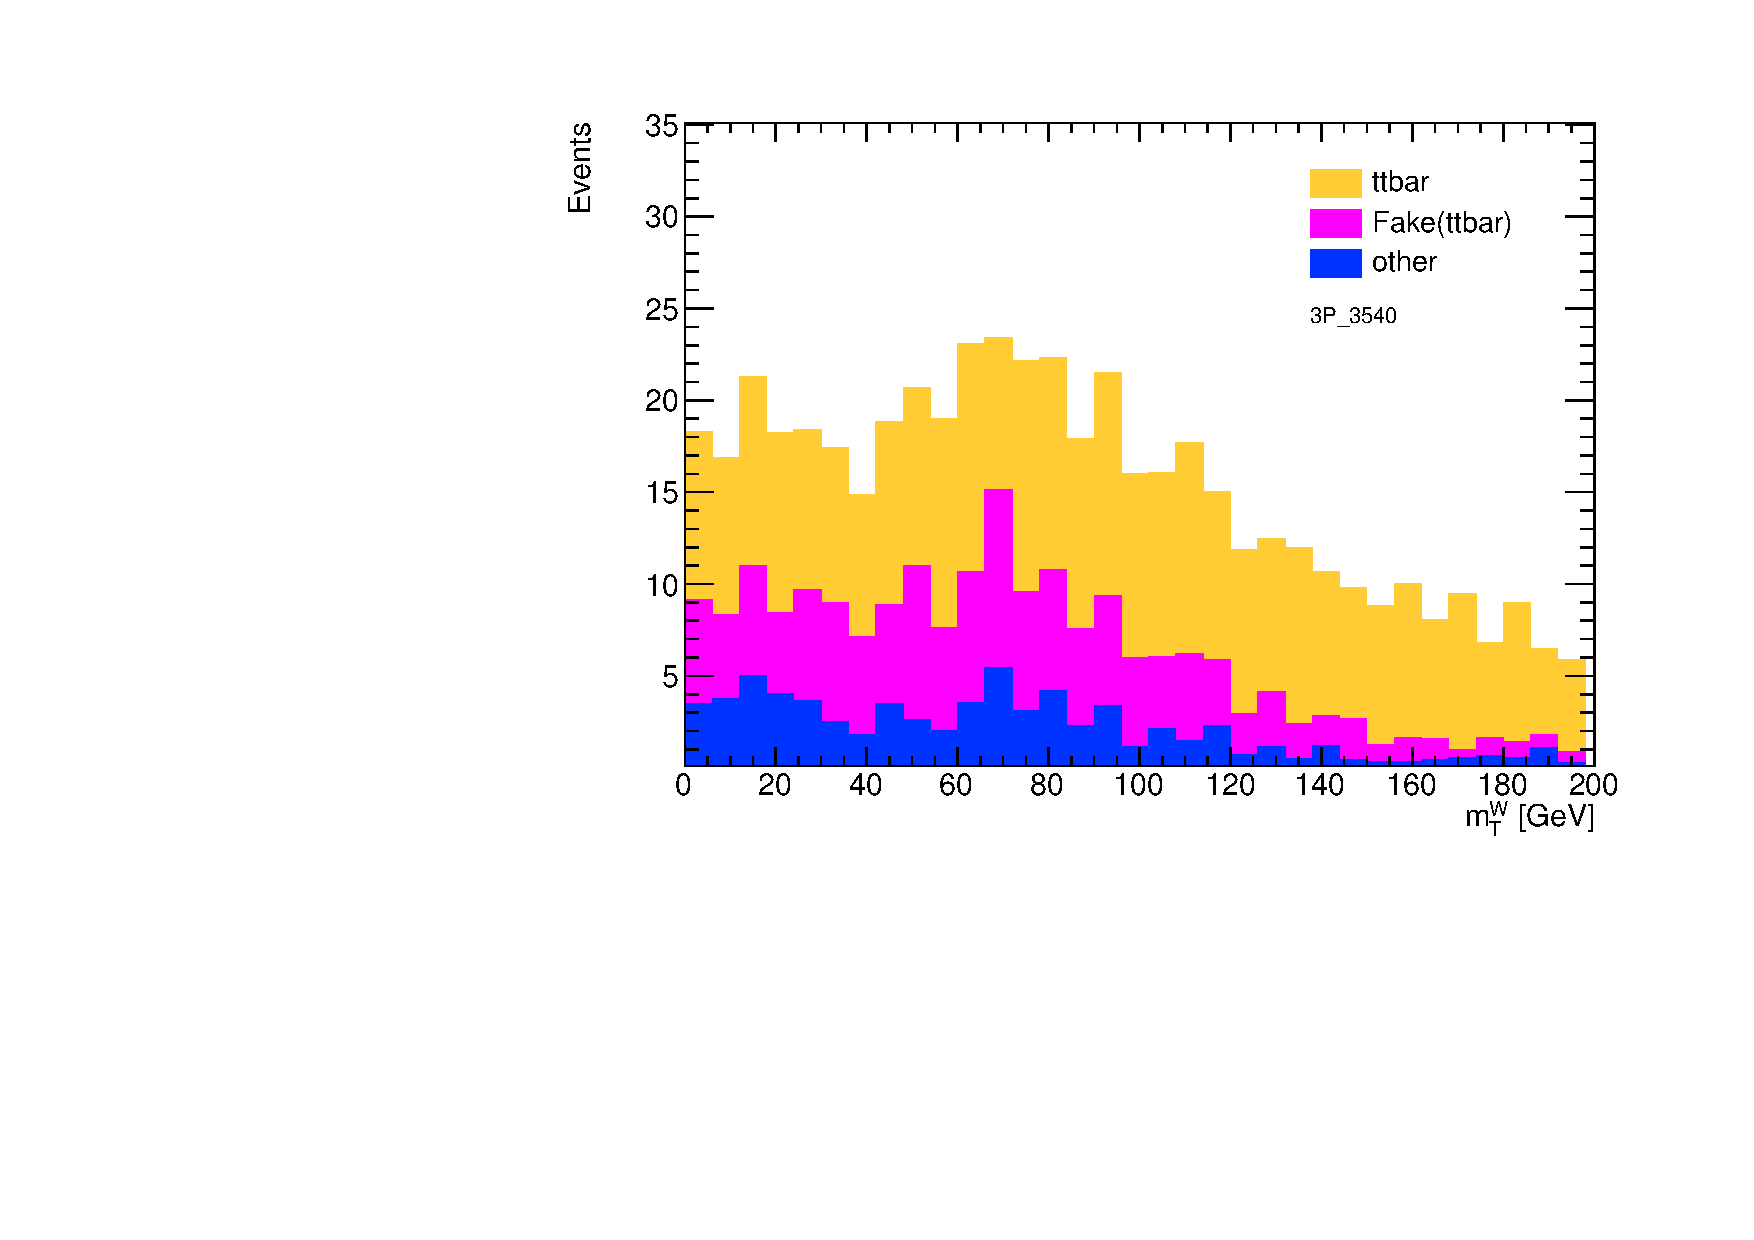
\includegraphics[scale=0.15]{mtw_fine_binning_stGE500LT600_3P_3540}}
        \subfloat[$40<p_T<45$] {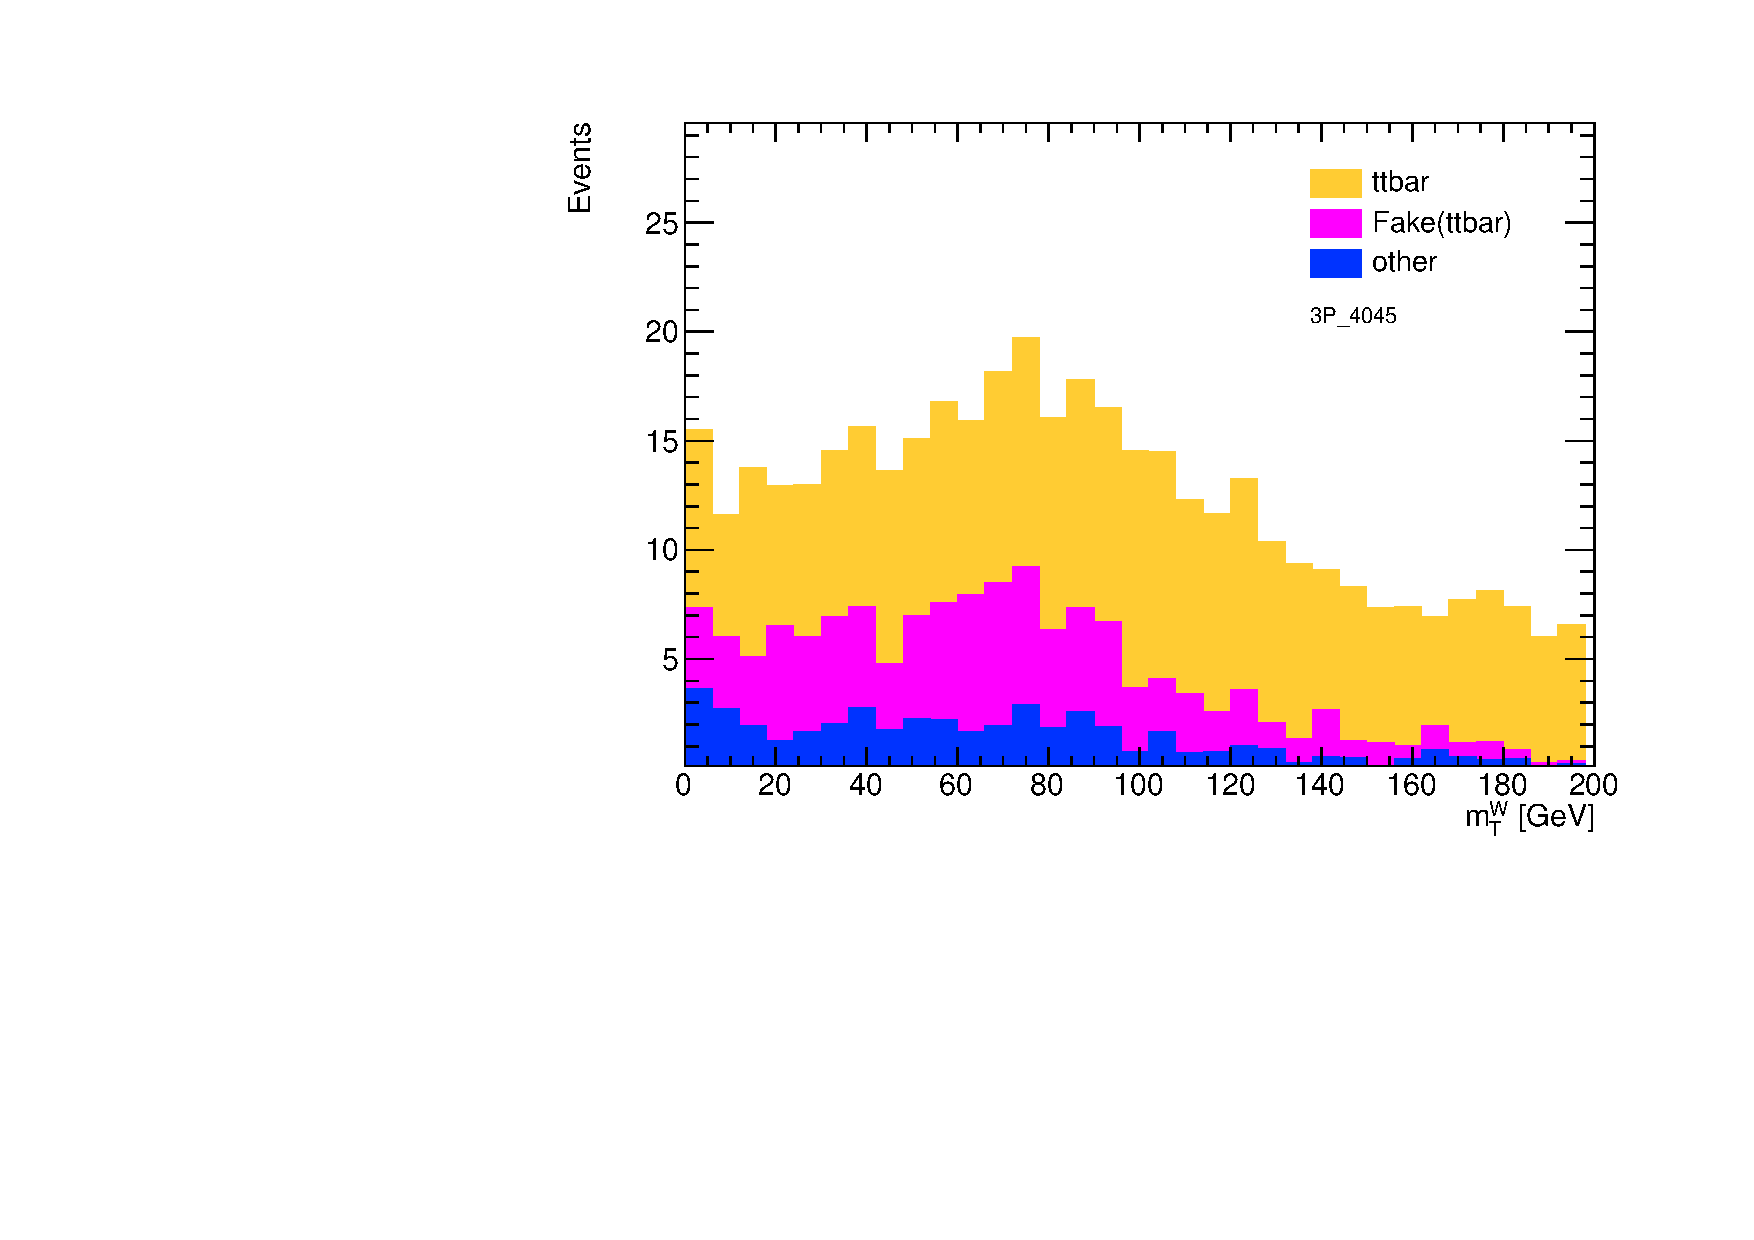
\includegraphics[scale=0.15]{mtw_fine_binning_stGE500LT600_3P_4045}}
        \subfloat[$45<p_T<50$] {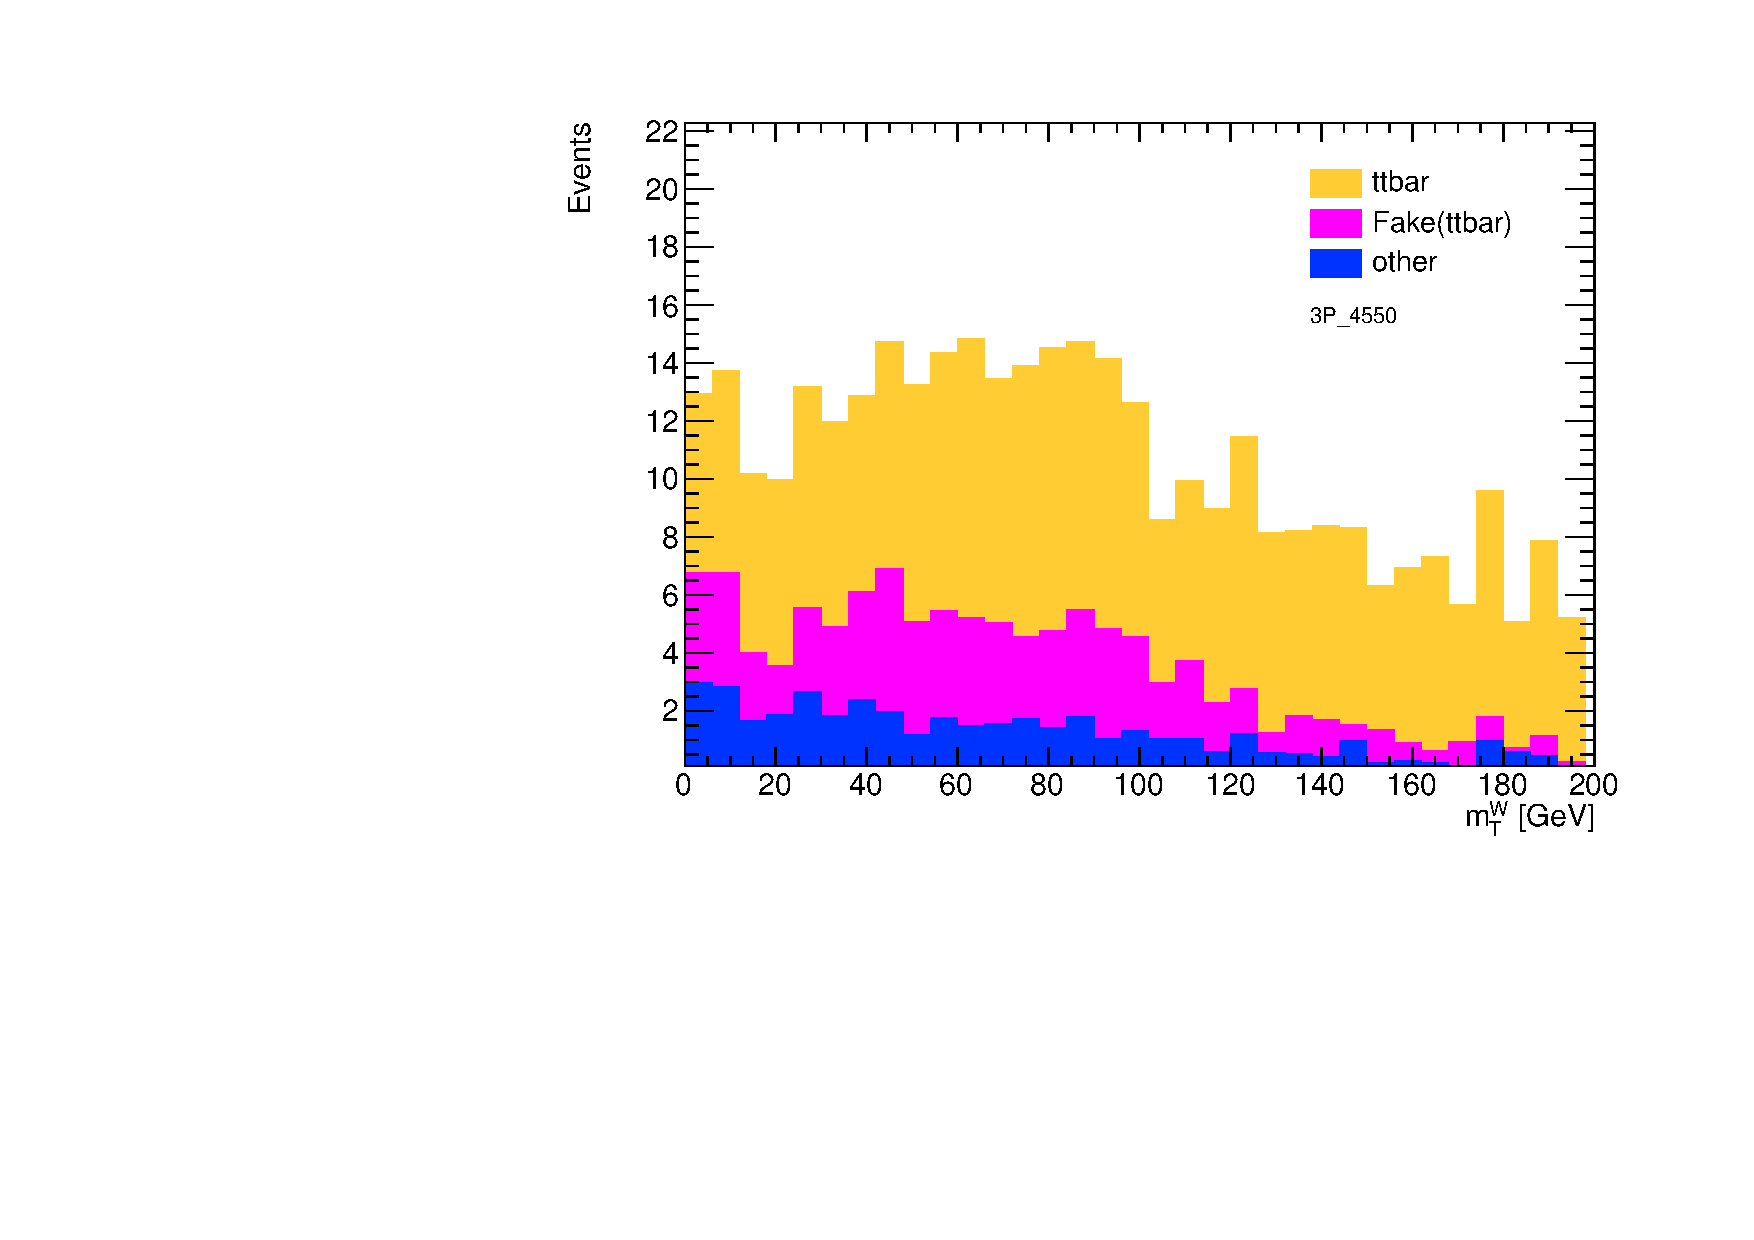
\includegraphics[scale=0.15]{mtw_fine_binning_stGE500LT600_3P_4550}} \\
        \subfloat[$50<p_T<55$] {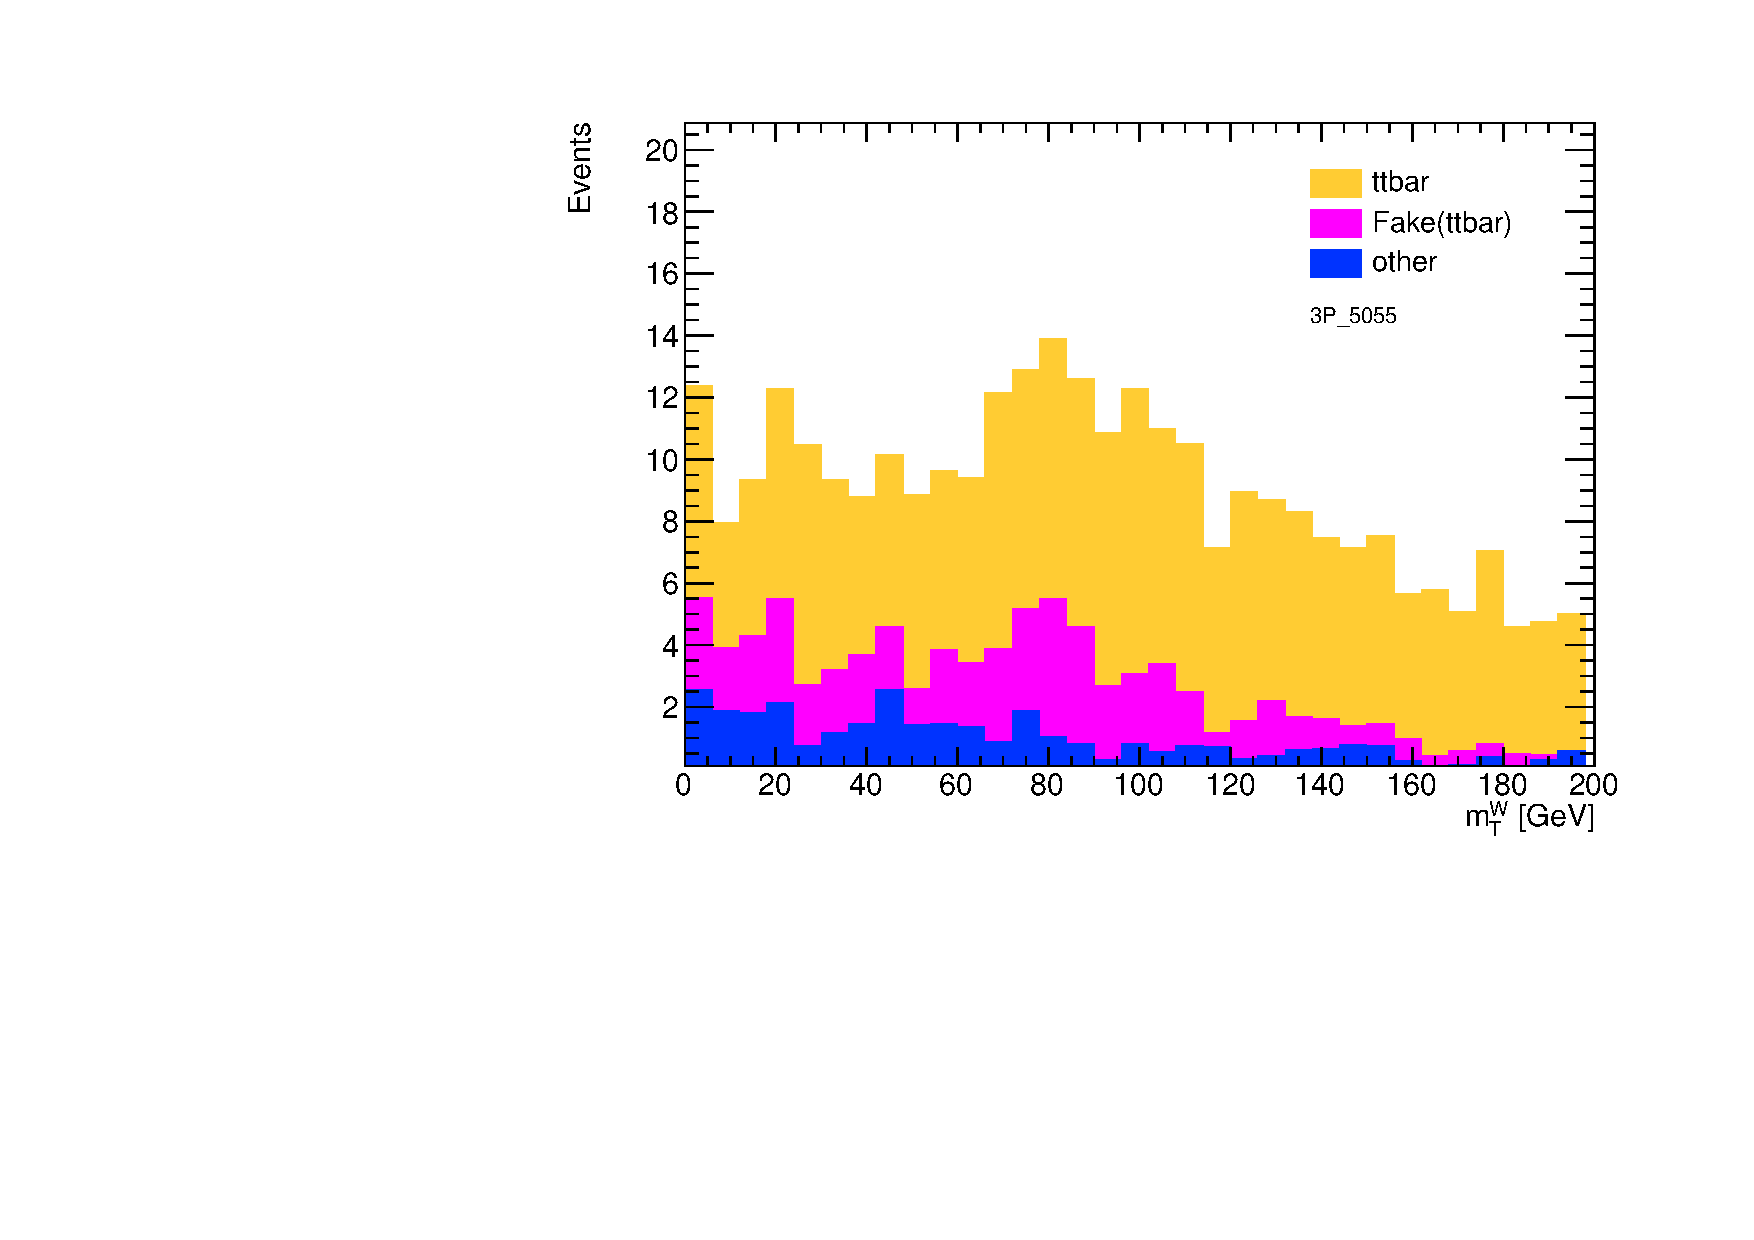
\includegraphics[scale=0.15]{mtw_fine_binning_stGE500LT600_3P_5055}}
        \subfloat[$55<p_T<70$] {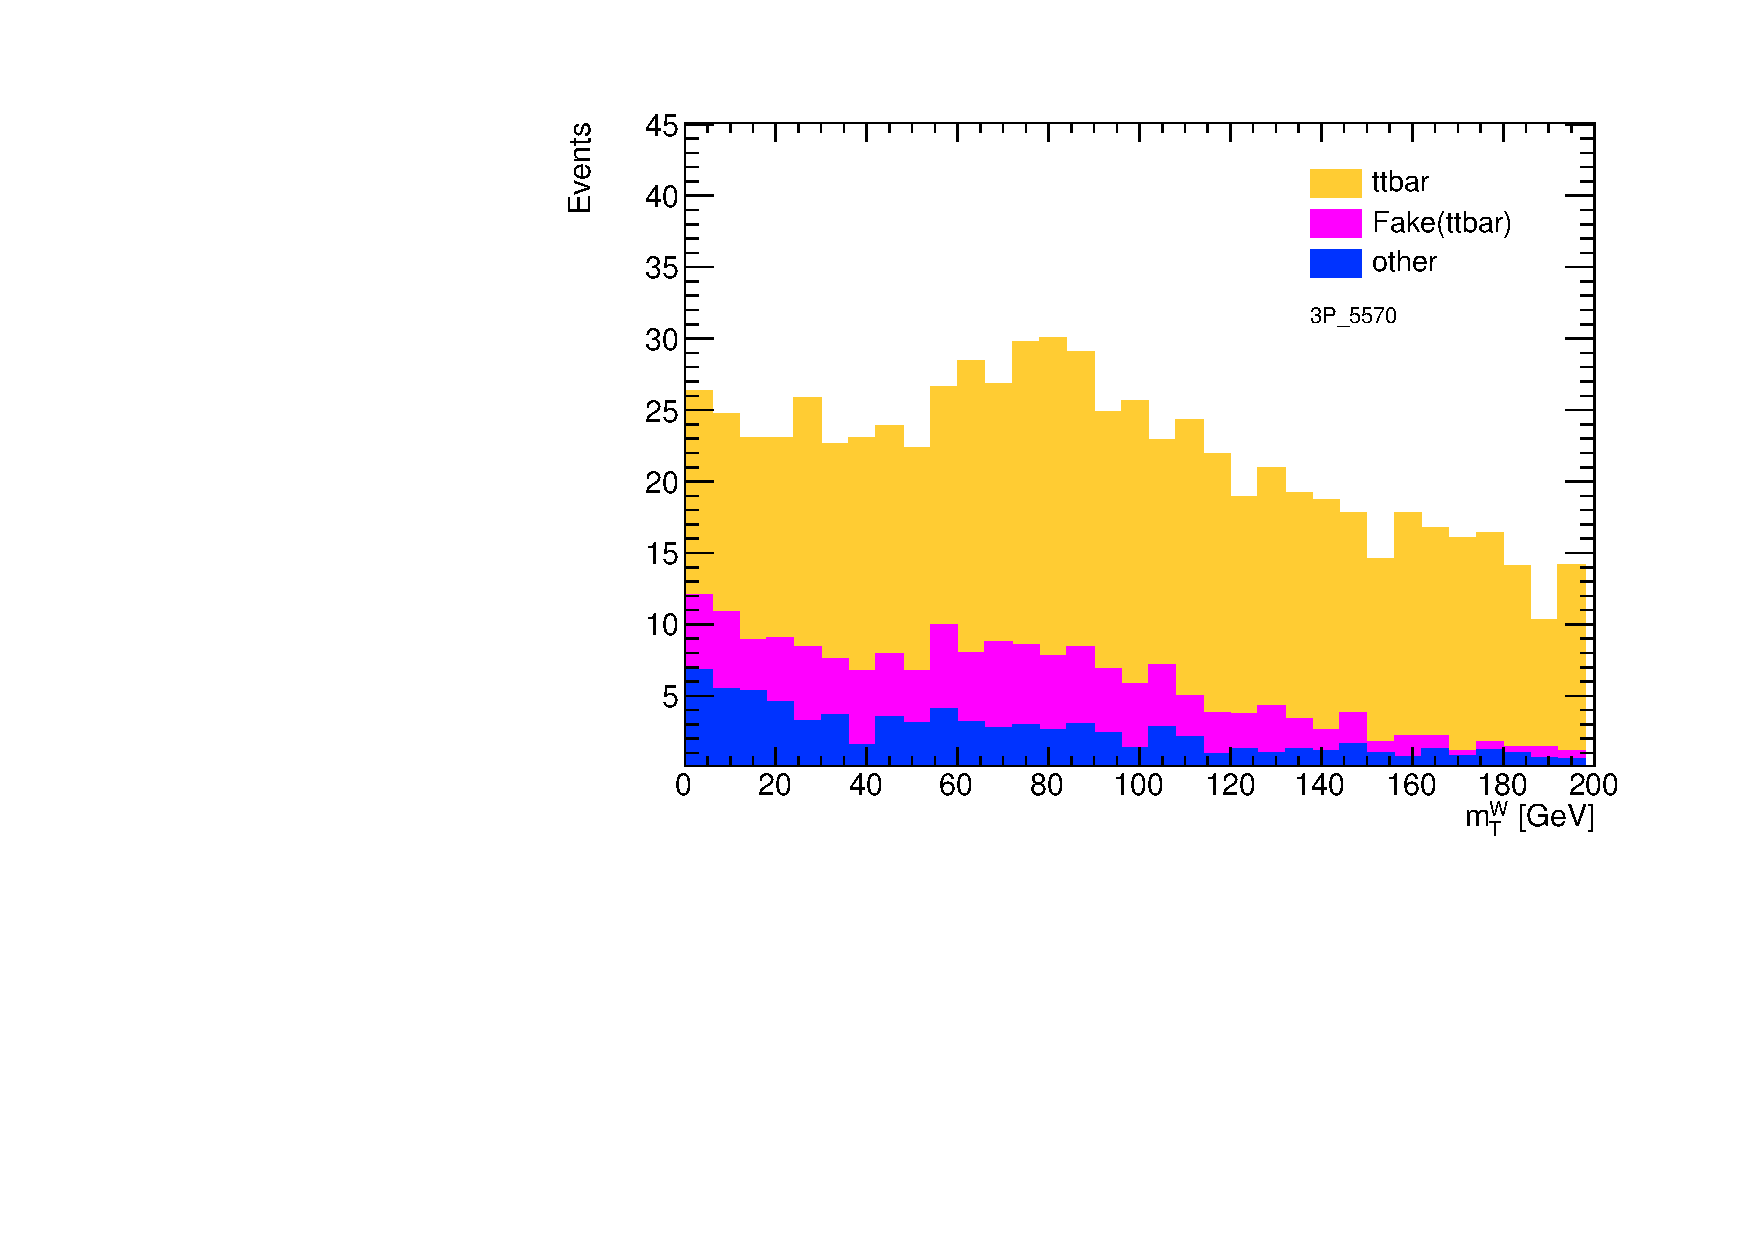
\includegraphics[scale=0.15]{mtw_fine_binning_stGE500LT600_3P_5570}}
        \subfloat[$70<p_T$]    {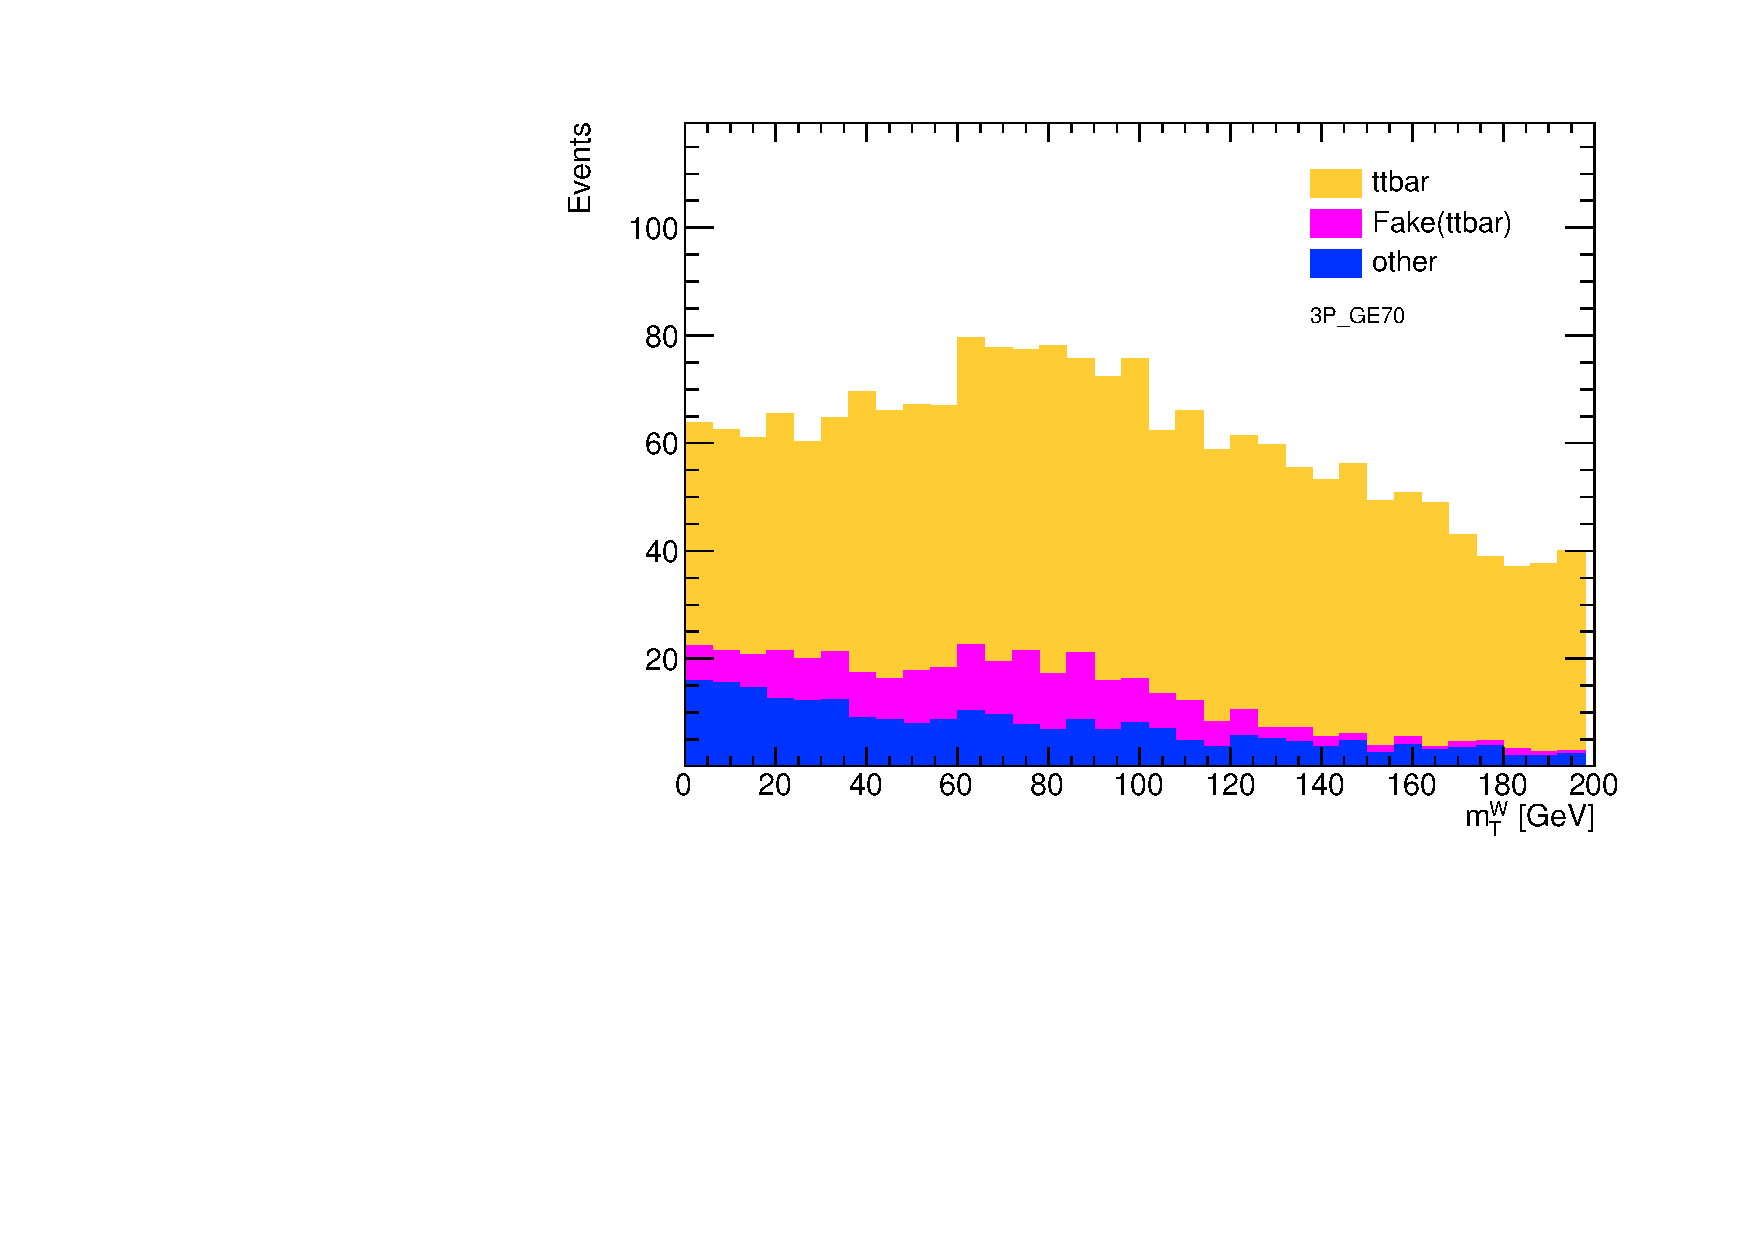
\includegraphics[scale=0.15]{mtw_fine_binning_stGE500LT600_3P_GE70}}
  \end{figure}       
\end{frame}



% ================================================================================================================= % 
\subtitlepage{Pre-fit Distributions (@CR1-3)}

\begin{frame}{Pre-fit Distributions (1-prong, CR1)}
  no trigger matching
  \begin{figure}
    \setcounter{subfigure}{0}
    \centering
        \subfloat[$p_T<35$]   {\includegraphics[scale=0.13]{stLT400/Region_BMin0_incJet1_dist1PLE35_J2_DMTW1PLE35notrigger_T2_SpcTauLH_Y2015_LTT0_L1_Prefit}}
        \subfloat[$35<p_T<40$]{\includegraphics[scale=0.13]{stLT400/Region_BMin0_incJet1_dist1P3540_J2_DMTW1P3540notrigger_T2_SpcTauLH_Y2015_LTT0_L1_Prefit}}
        \subfloat[$40<p_T<45$]{\includegraphics[scale=0.13]{stLT400/Region_BMin0_incJet1_dist1P4045_J2_DMTW1P4045notrigger_T2_SpcTauLH_Y2015_LTT0_L1_Prefit}}
        \subfloat[$45<p_T<50$]{\includegraphics[scale=0.13]{stLT400/Region_BMin0_incJet1_dist1P4550_J2_DMTW1P4550notrigger_T2_SpcTauLH_Y2015_LTT0_L1_Prefit}}
      \vspace{5mm}  
        \\          
        \subfloat[$50<p_T<55$] {\includegraphics[scale=0.13]{stLT400/Region_BMin0_incJet1_dist1P5055_J2_DMTW1P5055notrigger_T2_SpcTauLH_Y2015_LTT0_L1_Prefit}}
        \subfloat[$55<p_T<70$] {\includegraphics[scale=0.13]{stLT400/Region_BMin0_incJet1_dist1P5570_J2_DMTW1P5570notrigger_T2_SpcTauLH_Y2015_LTT0_L1_Prefit}}
        \subfloat[$70<p_T<100$]{\includegraphics[scale=0.13]{stLT400/Region_BMin0_incJet1_dist1P70100_J2_DMTW1P70100notrigger_T2_SpcTauLH_Y2015_LTT0_L1_Prefit}}
        \subfloat[$100<p_T$]   {\includegraphics[scale=0.13]{stLT400/Region_BMin0_incJet1_dist1PGE100_J2_DMTW1PGE100notrigger_T2_SpcTauLH_Y2015_LTT0_L1_Prefit}}
  \end{figure}
\end{frame}


\begin{frame}{Pre-fit Distributions (3-prong, CR1)}
  no trigger matching
  \begin{figure}
    \setcounter{subfigure}{0}
    \centering
        \subfloat[$p_T<35$]   {\includegraphics[scale=0.13]{stLT400/Region_BMin0_incJet1_dist3PLE35_J2_DMTW3PLE35notrigger_T2_SpcTauLH_Y2015_LTT0_L1_Prefit}}
        \subfloat[$35<p_T<40$]{\includegraphics[scale=0.13]{stLT400/Region_BMin0_incJet1_dist3P3540_J2_DMTW3P3540notrigger_T2_SpcTauLH_Y2015_LTT0_L1_Prefit}}
        \subfloat[$40<p_T<45$]{\includegraphics[scale=0.13]{stLT400/Region_BMin0_incJet1_dist3P4045_J2_DMTW3P4045notrigger_T2_SpcTauLH_Y2015_LTT0_L1_Prefit}}
        \subfloat[$45<p_T<50$]{\includegraphics[scale=0.13]{stLT400/Region_BMin0_incJet1_dist3P4550_J2_DMTW3P4550notrigger_T2_SpcTauLH_Y2015_LTT0_L1_Prefit}}
      \vspace{5mm}
        \\
        \subfloat[$50<p_T<55$]{\includegraphics[scale=0.13]{stLT400/Region_BMin0_incJet1_dist3P5055_J2_DMTW3P5055notrigger_T2_SpcTauLH_Y2015_LTT0_L1_Prefit}}
        \subfloat[$55<p_T<70$]{\includegraphics[scale=0.13]{stLT400/Region_BMin0_incJet1_dist3P5570_J2_DMTW3P5570notrigger_T2_SpcTauLH_Y2015_LTT0_L1_Prefit}}
        \subfloat[$70<p_T$]   {\includegraphics[scale=0.13]{stLT400/Region_BMin0_incJet1_dist3PGE70_J2_DMTW3PGE70notrigger_T2_SpcTauLH_Y2015_LTT0_L1_Prefit}}
  \end{figure}
\end{frame}

\begin{frame}{Pre-fit Distributions (1-prong, CR2)}
  no trigger matching
  \begin{figure}
    \setcounter{subfigure}{0}
    \centering
        \subfloat[$p_T<35$]   {\includegraphics[scale=0.13]{stGE400LT500/Region_BMin0_incJet1_dist1PLE35_J2_DMTW1PLE35notrigger_T2_SpcTauLH_Y2015_LTT0_L1_Prefit}}
        \subfloat[$35<p_T<40$]{\includegraphics[scale=0.13]{stGE400LT500/Region_BMin0_incJet1_dist1P3540_J2_DMTW1P3540notrigger_T2_SpcTauLH_Y2015_LTT0_L1_Prefit}}
        \subfloat[$40<p_T<45$]{\includegraphics[scale=0.13]{stGE400LT500/Region_BMin0_incJet1_dist1P4045_J2_DMTW1P4045notrigger_T2_SpcTauLH_Y2015_LTT0_L1_Prefit}}
        \subfloat[$45<p_T<50$]{\includegraphics[scale=0.13]{stGE400LT500/Region_BMin0_incJet1_dist1P4550_J2_DMTW1P4550notrigger_T2_SpcTauLH_Y2015_LTT0_L1_Prefit}}
      \vspace{5mm}
        \\
        \subfloat[$50<p_T<55$] {\includegraphics[scale=0.13]{stGE400LT500/Region_BMin0_incJet1_dist1P5055_J2_DMTW1P5055notrigger_T2_SpcTauLH_Y2015_LTT0_L1_Prefit}}
        \subfloat[$55<p_T<70$] {\includegraphics[scale=0.13]{stGE400LT500/Region_BMin0_incJet1_dist1P5570_J2_DMTW1P5570notrigger_T2_SpcTauLH_Y2015_LTT0_L1_Prefit}}
        \subfloat[$70<p_T<100$]{\includegraphics[scale=0.13]{stGE400LT500/Region_BMin0_incJet1_dist1P70100_J2_DMTW1P70100notrigger_T2_SpcTauLH_Y2015_LTT0_L1_Prefit}}
        \subfloat[$100<p_T$]   {\includegraphics[scale=0.13]{stGE400LT500/Region_BMin0_incJet1_dist1PGE100_J2_DMTW1PGE100notrigger_T2_SpcTauLH_Y2015_LTT0_L1_Prefit}}
  \end{figure}
\end{frame}


\begin{frame}{Pre-fit Distributions (3-prong, CR2)}
  no trigger matching
  \begin{figure}
    \setcounter{subfigure}{0}
    \centering
        \subfloat[$p_T<35$]   {\includegraphics[scale=0.13]{stGE400LT500/Region_BMin0_incJet1_dist3PLE35_J2_DMTW3PLE35notrigger_T2_SpcTauLH_Y2015_LTT0_L1_Prefit}}
        \subfloat[$35<p_T<40$]{\includegraphics[scale=0.13]{stGE400LT500/Region_BMin0_incJet1_dist3P3540_J2_DMTW3P3540notrigger_T2_SpcTauLH_Y2015_LTT0_L1_Prefit}}
        \subfloat[$40<p_T<45$]{\includegraphics[scale=0.13]{stGE400LT500/Region_BMin0_incJet1_dist3P4045_J2_DMTW3P4045notrigger_T2_SpcTauLH_Y2015_LTT0_L1_Prefit}}
        \subfloat[$45<p_T<50$]{\includegraphics[scale=0.13]{stGE400LT500/Region_BMin0_incJet1_dist3P4550_J2_DMTW3P4550notrigger_T2_SpcTauLH_Y2015_LTT0_L1_Prefit}}
      \vspace{5mm}
        \\
        \subfloat[$50<p_T<55$]{\includegraphics[scale=0.13]{stGE400LT500/Region_BMin0_incJet1_dist3P5055_J2_DMTW3P5055notrigger_T2_SpcTauLH_Y2015_LTT0_L1_Prefit}}
        \subfloat[$55<p_T<70$]{\includegraphics[scale=0.13]{stGE400LT500/Region_BMin0_incJet1_dist3P5570_J2_DMTW3P5570notrigger_T2_SpcTauLH_Y2015_LTT0_L1_Prefit}}
        \subfloat[$70<p_T$]   {\includegraphics[scale=0.13]{stGE400LT500/Region_BMin0_incJet1_dist3PGE70_J2_DMTW3PGE70notrigger_T2_SpcTauLH_Y2015_LTT0_L1_Prefit}}
  \end{figure}
\end{frame}

\begin{frame}{Pre-fit Distributions (1-prong, CR3)}
  no trigger matching
  \begin{figure}
    \setcounter{subfigure}{0}
    \centering
        \subfloat[$p_T<35$]   {\includegraphics[scale=0.13]{stGE500LT600/Region_BMin0_incJet1_dist1PLE35_J2_DMTW1PLE35notrigger_T2_SpcTauLH_Y2015_LTT0_L1_Prefit}}
        \subfloat[$35<p_T<40$]{\includegraphics[scale=0.13]{stGE500LT600/Region_BMin0_incJet1_dist1P3540_J2_DMTW1P3540notrigger_T2_SpcTauLH_Y2015_LTT0_L1_Prefit}}
        \subfloat[$40<p_T<45$]{\includegraphics[scale=0.13]{stGE500LT600/Region_BMin0_incJet1_dist1P4045_J2_DMTW1P4045notrigger_T2_SpcTauLH_Y2015_LTT0_L1_Prefit}}
        \subfloat[$45<p_T<50$]{\includegraphics[scale=0.13]{stGE500LT600/Region_BMin0_incJet1_dist1P4550_J2_DMTW1P4550notrigger_T2_SpcTauLH_Y2015_LTT0_L1_Prefit}}
      \vspace{5mm}
        \\
        \subfloat[$50<p_T<55$] {\includegraphics[scale=0.13]{stGE500LT600/Region_BMin0_incJet1_dist1P5055_J2_DMTW1P5055notrigger_T2_SpcTauLH_Y2015_LTT0_L1_Prefit}}
        \subfloat[$55<p_T<70$] {\includegraphics[scale=0.13]{stGE500LT600/Region_BMin0_incJet1_dist1P5570_J2_DMTW1P5570notrigger_T2_SpcTauLH_Y2015_LTT0_L1_Prefit}}
        \subfloat[$70<p_T<100$]{\includegraphics[scale=0.13]{stGE500LT600/Region_BMin0_incJet1_dist1P70100_J2_DMTW1P70100notrigger_T2_SpcTauLH_Y2015_LTT0_L1_Prefit}}
        \subfloat[$100<p_T$]   {\includegraphics[scale=0.13]{stGE500LT600/Region_BMin0_incJet1_dist1PGE100_J2_DMTW1PGE100notrigger_T2_SpcTauLH_Y2015_LTT0_L1_Prefit}}
  \end{figure}
\end{frame}

\begin{frame}{Pre-fit Distributions (3-prong, CR3)}
  no trigger matching
  \begin{figure}
    \setcounter{subfigure}{0}
    \centering
        \subfloat[$p_T<35$]   {\includegraphics[scale=0.13]{stGE500LT600/Region_BMin0_incJet1_dist3PLE35_J2_DMTW3PLE35notrigger_T2_SpcTauLH_Y2015_LTT0_L1_Prefit}}
        \subfloat[$35<p_T<40$]{\includegraphics[scale=0.13]{stGE500LT600/Region_BMin0_incJet1_dist3P3540_J2_DMTW3P3540notrigger_T2_SpcTauLH_Y2015_LTT0_L1_Prefit}}
        \subfloat[$40<p_T<45$]{\includegraphics[scale=0.13]{stGE500LT600/Region_BMin0_incJet1_dist3P4045_J2_DMTW3P4045notrigger_T2_SpcTauLH_Y2015_LTT0_L1_Prefit}}
        \subfloat[$45<p_T<50$]{\includegraphics[scale=0.13]{stGE500LT600/Region_BMin0_incJet1_dist3P4550_J2_DMTW3P4550notrigger_T2_SpcTauLH_Y2015_LTT0_L1_Prefit}}
      \vspace{5mm}
        \\
        \subfloat[$50<p_T<55$]{\includegraphics[scale=0.13]{stGE500LT600/Region_BMin0_incJet1_dist3P5055_J2_DMTW3P5055notrigger_T2_SpcTauLH_Y2015_LTT0_L1_Prefit}}
        \subfloat[$55<p_T<70$]{\includegraphics[scale=0.13]{stGE500LT600/Region_BMin0_incJet1_dist3P5570_J2_DMTW3P5570notrigger_T2_SpcTauLH_Y2015_LTT0_L1_Prefit}}
        \subfloat[$70<p_T$]   {\includegraphics[scale=0.13]{stGE500LT600/Region_BMin0_incJet1_dist3PGE70_J2_DMTW3PGE70notrigger_T2_SpcTauLH_Y2015_LTT0_L1_Prefit}}
  \end{figure}
\end{frame}

\subtitlepage{Post-fit Results (@CR1-3)}

\begin{frame}{Fake SF (\sT slice)}\label{fake_sf_cr1_cr2_c3}
  \vspace{5mm}
  \begin{figure}
    \setcounter{subfigure}{0}
    \centering
        \includegraphics[scale=0.29]{scale_factor_controlregions_1P_notrigger}
        \includegraphics[scale=0.29]{scale_factor_controlregions_3P_notrigger}
  \end{figure}

  \begin{itemize}
    \item The 3-prong SF has larger errors than the 1-prong's.
  \end{itemize}
\end{frame}


\begin{frame}{Post-fit Distributions (1-prong, CR1)}
  no trigger matching
  \begin{figure}
    \setcounter{subfigure}{0}
    \centering
        \subfloat[$p_T<35$]   {\includegraphics[scale=0.13]{stLT400/Region_BMin0_incJet1_dist1PLE35_J2_DMTW1PLE35notrigger_T2_SpcTauLH_Y2015_LTT0_L1_GlobalFit_unconditionnal_mu1}}
        \subfloat[$35<p_T<40$]{\includegraphics[scale=0.13]{stLT400/Region_BMin0_incJet1_dist1P3540_J2_DMTW1P3540notrigger_T2_SpcTauLH_Y2015_LTT0_L1_GlobalFit_unconditionnal_mu1}}
        \subfloat[$40<p_T<45$]{\includegraphics[scale=0.13]{stLT400/Region_BMin0_incJet1_dist1P4045_J2_DMTW1P4045notrigger_T2_SpcTauLH_Y2015_LTT0_L1_GlobalFit_unconditionnal_mu1}}
        \subfloat[$45<p_T<50$]{\includegraphics[scale=0.13]{stLT400/Region_BMin0_incJet1_dist1P4550_J2_DMTW1P4550notrigger_T2_SpcTauLH_Y2015_LTT0_L1_GlobalFit_unconditionnal_mu1}}
      \vspace{5mm}
        \\
        \subfloat[$50<p_T<55$] {\includegraphics[scale=0.13]{stLT400/Region_BMin0_incJet1_dist1P5055_J2_DMTW1P5055notrigger_T2_SpcTauLH_Y2015_LTT0_L1_GlobalFit_unconditionnal_mu1}}
        \subfloat[$55<p_T<70$] {\includegraphics[scale=0.13]{stLT400/Region_BMin0_incJet1_dist1P5570_J2_DMTW1P5570notrigger_T2_SpcTauLH_Y2015_LTT0_L1_GlobalFit_unconditionnal_mu1}}
        \subfloat[$70<p_T<100$]{\includegraphics[scale=0.13]{stLT400/Region_BMin0_incJet1_dist1P70100_J2_DMTW1P70100notrigger_T2_SpcTauLH_Y2015_LTT0_L1_GlobalFit_unconditionnal_mu1}}
        \subfloat[$100<p_T$]   {\includegraphics[scale=0.13]{stLT400/Region_BMin0_incJet1_dist1PGE100_J2_DMTW1PGE100notrigger_T2_SpcTauLH_Y2015_LTT0_L1_GlobalFit_unconditionnal_mu1}}
  \end{figure}
\end{frame}

\begin{frame}{Post-fit Distributions (3-prong, CR1)}
  no trigger matching
  \begin{figure}
    \setcounter{subfigure}{0}
    \centering
        \subfloat[$p_T<35$]   {\includegraphics[scale=0.13]{stLT400/Region_BMin0_incJet1_dist3PLE35_J2_DMTW3PLE35notrigger_T2_SpcTauLH_Y2015_LTT0_L1_GlobalFit_unconditionnal_mu1}}
        \subfloat[$35<p_T<40$]{\includegraphics[scale=0.13]{stLT400/Region_BMin0_incJet1_dist3P3540_J2_DMTW3P3540notrigger_T2_SpcTauLH_Y2015_LTT0_L1_GlobalFit_unconditionnal_mu1}}
        \subfloat[$40<p_T<45$]{\includegraphics[scale=0.13]{stLT400/Region_BMin0_incJet1_dist3P4045_J2_DMTW3P4045notrigger_T2_SpcTauLH_Y2015_LTT0_L1_GlobalFit_unconditionnal_mu1}}
        \subfloat[$45<p_T<50$]{\includegraphics[scale=0.13]{stLT400/Region_BMin0_incJet1_dist3P4550_J2_DMTW3P4550notrigger_T2_SpcTauLH_Y2015_LTT0_L1_GlobalFit_unconditionnal_mu1}}
      \vspace{5mm}
        \\
        \subfloat[$50<p_T<55$]{\includegraphics[scale=0.13]{stLT400/Region_BMin0_incJet1_dist3P5055_J2_DMTW3P5055notrigger_T2_SpcTauLH_Y2015_LTT0_L1_GlobalFit_unconditionnal_mu1}}
        \subfloat[$55<p_T<70$]{\includegraphics[scale=0.13]{stLT400/Region_BMin0_incJet1_dist3P5570_J2_DMTW3P5570notrigger_T2_SpcTauLH_Y2015_LTT0_L1_GlobalFit_unconditionnal_mu1}}
        \subfloat[$70<p_T$]   {\includegraphics[scale=0.13]{stLT400/Region_BMin0_incJet1_dist3PGE70_J2_DMTW3PGE70notrigger_T2_SpcTauLH_Y2015_LTT0_L1_GlobalFit_unconditionnal_mu1}}
  \end{figure}
\end{frame}

\begin{frame}{Post-fit Pulls (CR1)}
  \begin{figure}
    \includegraphics[scale=0.3]{pull_pulls_stLT400}
  \end{figure}
\end{frame}

\begin{frame}{Correlations of all NPs (CR1)}
  \vspace{15mm}
  \begin{figure}
    \setcounter{subfigure}{0}
    \centering
        \subfloat[1-prong]{\includegraphics[scale=0.29]{correlation_1P_notrigger_CR1_stLT400}}
        \subfloat[3-prong]{\includegraphics[scale=0.29]{correlation_3P_notrigger_CR1_stLT400}}
  \end{figure}
\end{frame}

\begin{frame}{Correlations of TTBar SFs (CR1)}
  \vspace{15mm}
  \begin{figure}
    \setcounter{subfigure}{0}
    \centering
        \subfloat[1-prong]{\includegraphics[scale=0.29]{correlation_sf_1P_notrigger_CR1_stLT400}}
        \subfloat[3-prong]{\includegraphics[scale=0.29]{correlation_sf_3P_notrigger_CR1_stLT400}}
  \end{figure}
\end{frame}

\begin{frame}{Post-fit Distributions (1-prong, CR2)}
  no trigger matching
  \begin{figure}
    \setcounter{subfigure}{0}
    \centering
    \subfloat[$p_T<35$]   {\includegraphics[scale=0.13]{stGE400LT500/Region_BMin0_incJet1_dist1PLE35_J2_DMTW1PLE35notrigger_T2_SpcTauLH_Y2015_LTT0_L1_GlobalFit_unconditionnal_mu1}}
    \subfloat[$35<p_T<40$]{\includegraphics[scale=0.13]{stGE400LT500/Region_BMin0_incJet1_dist1P3540_J2_DMTW1P3540notrigger_T2_SpcTauLH_Y2015_LTT0_L1_GlobalFit_unconditionnal_mu1}}
    \subfloat[$40<p_T<45$]{\includegraphics[scale=0.13]{stGE400LT500/Region_BMin0_incJet1_dist1P4045_J2_DMTW1P4045notrigger_T2_SpcTauLH_Y2015_LTT0_L1_GlobalFit_unconditionnal_mu1}}
    \subfloat[$45<p_T<50$]{\includegraphics[scale=0.13]{stGE400LT500/Region_BMin0_incJet1_dist1P4550_J2_DMTW1P4550notrigger_T2_SpcTauLH_Y2015_LTT0_L1_GlobalFit_unconditionnal_mu1}}
    \vspace{5mm}
    \\
    \subfloat[$50<p_T<55$] {\includegraphics[scale=0.13]{stGE400LT500/Region_BMin0_incJet1_dist1P5055_J2_DMTW1P5055notrigger_T2_SpcTauLH_Y2015_LTT0_L1_GlobalFit_unconditionnal_mu1}}
    \subfloat[$55<p_T<70$] {\includegraphics[scale=0.13]{stGE400LT500/Region_BMin0_incJet1_dist1P5570_J2_DMTW1P5570notrigger_T2_SpcTauLH_Y2015_LTT0_L1_GlobalFit_unconditionnal_mu1}}
    \subfloat[$70<p_T<100$]{\includegraphics[scale=0.13]{stGE400LT500/Region_BMin0_incJet1_dist1P70100_J2_DMTW1P70100notrigger_T2_SpcTauLH_Y2015_LTT0_L1_GlobalFit_unconditionnal_mu1}}
    \subfloat[$100<p_T$]   {\includegraphics[scale=0.13]{stGE400LT500/Region_BMin0_incJet1_dist1PGE100_J2_DMTW1PGE100notrigger_T2_SpcTauLH_Y2015_LTT0_L1_GlobalFit_unconditionnal_mu1}}
  \end{figure}
\end{frame}

\begin{frame}{Post-fit Distributions (3-prong, $CR2$)}
  no trigger matching
  \begin{figure}
    \setcounter{subfigure}{0}
    \centering
        \subfloat[$p_T<35$]   {\includegraphics[scale=0.13]{stGE400LT500/Region_BMin0_incJet1_dist3PLE35_J2_DMTW3PLE35notrigger_T2_SpcTauLH_Y2015_LTT0_L1_GlobalFit_unconditionnal_mu1}}
        \subfloat[$35<p_T<40$]{\includegraphics[scale=0.13]{stGE400LT500/Region_BMin0_incJet1_dist3P3540_J2_DMTW3P3540notrigger_T2_SpcTauLH_Y2015_LTT0_L1_GlobalFit_unconditionnal_mu1}}
        \subfloat[$40<p_T<45$]{\includegraphics[scale=0.13]{stGE400LT500/Region_BMin0_incJet1_dist3P4045_J2_DMTW3P4045notrigger_T2_SpcTauLH_Y2015_LTT0_L1_GlobalFit_unconditionnal_mu1}}
        \subfloat[$45<p_T<50$]{\includegraphics[scale=0.13]{stGE400LT500/Region_BMin0_incJet1_dist3P4550_J2_DMTW3P4550notrigger_T2_SpcTauLH_Y2015_LTT0_L1_GlobalFit_unconditionnal_mu1}}
      \vspace{5mm}
        \\
        \subfloat[$50<p_T<55$]{\includegraphics[scale=0.13]{stGE400LT500/Region_BMin0_incJet1_dist3P5055_J2_DMTW3P5055notrigger_T2_SpcTauLH_Y2015_LTT0_L1_GlobalFit_unconditionnal_mu1}}
        \subfloat[$55<p_T<70$]{\includegraphics[scale=0.13]{stGE400LT500/Region_BMin0_incJet1_dist3P5570_J2_DMTW3P5570notrigger_T2_SpcTauLH_Y2015_LTT0_L1_GlobalFit_unconditionnal_mu1}}
        \subfloat[$70<p_T$]   {\includegraphics[scale=0.13]{stGE400LT500/Region_BMin0_incJet1_dist3PGE70_J2_DMTW3PGE70notrigger_T2_SpcTauLH_Y2015_LTT0_L1_GlobalFit_unconditionnal_mu1}}
  \end{figure}
\end{frame}

\begin{frame}{Post-fit Pulls (CR2)}
  \begin{figure}
    \includegraphics[scale=0.3]{pull_pulls_stGE400LT500}
  \end{figure}
\end{frame}


\begin{frame}{Correlations of all NPs (CR2)}
  \vspace{15mm}
  \begin{figure}
    \setcounter{subfigure}{0}
    \centering
        \includegraphics[scale=0.29]{correlation_1P_notrigger_CR2_stGE400LT500}
        \includegraphics[scale=0.29]{correlation_3P_notrigger_CR2_stGE400LT500}
  \end{figure}
\end{frame}

\begin{frame}{Correlations of TTBar SFs (CR2)}
  \vspace{15mm}
  \begin{figure}
    \setcounter{subfigure}{0}
    \centering
        \includegraphics[scale=0.29]{correlation_sf_1P_notrigger_CR2_stGE400LT500}
        \includegraphics[scale=0.29]{correlation_sf_3P_notrigger_CR2_stGE400LT500}
  \end{figure}
\end{frame}


\begin{frame}{Post-fit Distributions (1-prong, CR3)}
  no trigger matching
  \begin{figure}
    \setcounter{subfigure}{0}
    \centering
        \subfloat[$p_T<35$]   {\includegraphics[scale=0.13]{stGE500LT600/Region_BMin0_incJet1_dist1PLE35_J2_DMTW1PLE35notrigger_T2_SpcTauLH_Y2015_LTT0_L1_GlobalFit_unconditionnal_mu1}}
        \subfloat[$35<p_T<40$]{\includegraphics[scale=0.13]{stGE500LT600/Region_BMin0_incJet1_dist1P3540_J2_DMTW1P3540notrigger_T2_SpcTauLH_Y2015_LTT0_L1_GlobalFit_unconditionnal_mu1}}
        \subfloat[$40<p_T<45$]{\includegraphics[scale=0.13]{stGE500LT600/Region_BMin0_incJet1_dist1P4045_J2_DMTW1P4045notrigger_T2_SpcTauLH_Y2015_LTT0_L1_GlobalFit_unconditionnal_mu1}}
        \subfloat[$45<p_T<50$]{\includegraphics[scale=0.13]{stGE500LT600/Region_BMin0_incJet1_dist1P4550_J2_DMTW1P4550notrigger_T2_SpcTauLH_Y2015_LTT0_L1_GlobalFit_unconditionnal_mu1}}
      \vspace{5mm}
        \\
        \subfloat[$50<p_T<55$] {\includegraphics[scale=0.13]{stGE500LT600/Region_BMin0_incJet1_dist1P5055_J2_DMTW1P5055notrigger_T2_SpcTauLH_Y2015_LTT0_L1_GlobalFit_unconditionnal_mu1}}
        \subfloat[$55<p_T<70$] {\includegraphics[scale=0.13]{stGE500LT600/Region_BMin0_incJet1_dist1P5570_J2_DMTW1P5570notrigger_T2_SpcTauLH_Y2015_LTT0_L1_GlobalFit_unconditionnal_mu1}}
        \subfloat[$70<p_T<100$]{\includegraphics[scale=0.13]{stGE500LT600/Region_BMin0_incJet1_dist1P70100_J2_DMTW1P70100notrigger_T2_SpcTauLH_Y2015_LTT0_L1_GlobalFit_unconditionnal_mu1}}
        \subfloat[$100<p_T$]   {\includegraphics[scale=0.13]{stGE500LT600/Region_BMin0_incJet1_dist1PGE100_J2_DMTW1PGE100notrigger_T2_SpcTauLH_Y2015_LTT0_L1_GlobalFit_unconditionnal_mu1}}
  \end{figure}
\end{frame}

\begin{frame}{Post-fit Distributions (3-prong, CR3)}
  no trigger matching
  \begin{figure}
    \setcounter{subfigure}{0}
    \centering
        \subfloat[$p_T<35$]   {\includegraphics[scale=0.13]{stGE500LT600/Region_BMin0_incJet1_dist3PLE35_J2_DMTW3PLE35notrigger_T2_SpcTauLH_Y2015_LTT0_L1_GlobalFit_unconditionnal_mu1}}
        \subfloat[$35<p_T<40$]{\includegraphics[scale=0.13]{stGE500LT600/Region_BMin0_incJet1_dist3P3540_J2_DMTW3P3540notrigger_T2_SpcTauLH_Y2015_LTT0_L1_GlobalFit_unconditionnal_mu1}}
        \subfloat[$40<p_T<45$]{\includegraphics[scale=0.13]{stGE500LT600/Region_BMin0_incJet1_dist3P4045_J2_DMTW3P4045notrigger_T2_SpcTauLH_Y2015_LTT0_L1_GlobalFit_unconditionnal_mu1}}
        \subfloat[$45<p_T<50$]{\includegraphics[scale=0.13]{stGE500LT600/Region_BMin0_incJet1_dist3P4550_J2_DMTW3P4550notrigger_T2_SpcTauLH_Y2015_LTT0_L1_GlobalFit_unconditionnal_mu1}}
      \vspace{5mm}
        \\
        \subfloat[$50<p_T<55$]{\includegraphics[scale=0.13]{stGE500LT600/Region_BMin0_incJet1_dist3P5055_J2_DMTW3P5055notrigger_T2_SpcTauLH_Y2015_LTT0_L1_GlobalFit_unconditionnal_mu1}}
        \subfloat[$55<p_T<70$]{\includegraphics[scale=0.13]{stGE500LT600/Region_BMin0_incJet1_dist3P5570_J2_DMTW3P5570notrigger_T2_SpcTauLH_Y2015_LTT0_L1_GlobalFit_unconditionnal_mu1}}
        \subfloat[$70<p_T$]   {\includegraphics[scale=0.13]{stGE500LT600/Region_BMin0_incJet1_dist3PGE70_J2_DMTW3PGE70notrigger_T2_SpcTauLH_Y2015_LTT0_L1_GlobalFit_unconditionnal_mu1}}
  \end{figure}
\end{frame}

\begin{frame}{Post-fit Pulls (CR3)}
  \begin{figure}
    \includegraphics[scale=0.3]{pull_pulls_stGE500LT600}
  \end{figure}
\end{frame}

\begin{frame}{Correlations of all NPs (CR3)}
  \vspace{15mm}
  \begin{figure}
    \setcounter{subfigure}{0}
    \centering
        \includegraphics[scale=0.29]{correlation_1P_notrigger_CR3_stGE500LT600}
        \includegraphics[scale=0.29]{correlation_3P_notrigger_CR3_stGE500LT600}
  \end{figure}
\end{frame}

\begin{frame}{Correlations of TTBar SFs (CR3)}
  \vspace{15mm}
  \begin{figure}
    \setcounter{subfigure}{0}
    \centering
        \includegraphics[scale=0.29]{correlation_sf_1P_notrigger_CR3_stGE500LT600}
        \includegraphics[scale=0.29]{correlation_sf_3P_notrigger_CR3_stGE500LT600}
  \end{figure}
\end{frame}


\begin{frame}{Summary of the CR1-3 studies}
  \begin{itemize}
    \item These studies aimed to evaluate the \sT dependencies of the fake SF,  \\
      and estimate systematics to cover the effects.
    \item The investigated items :
      \begin{itemize}
        \item The SF differenceses as a function of \tauhad \pT \hyperlink{fake_sf_cr1_cr2_c3}{\beamerbutton{jump}}.
      \end{itemize}

      \vspp
    \item Open items :
      \begin{itemize}
        \item The systematics estimations 
        \item Do you have any good ideas?
      \end{itemize}
  \end{itemize}
\end{frame}


% ================================================================================================================= % 
\subtitlepage{Pre-fit Distributions (@CR0)}


\begin{frame}{Pre-fit Distributions (1-prong)}
  no trigger matching
  \begin{figure}
    \setcounter{subfigure}{0}
    \centering
        \subfloat[$p_T<35$]   {\includegraphics[scale=0.13]{stLT600/Region_BMin0_incJet1_dist1PLE35_J2_DMTW1PLE35notrigger_T2_SpcTauLH_Y2015_LTT0_L1_Prefit}}
        \subfloat[$35<p_T<40$]{\includegraphics[scale=0.13]{stLT600/Region_BMin0_incJet1_dist1P3540_J2_DMTW1P3540notrigger_T2_SpcTauLH_Y2015_LTT0_L1_Prefit}}
        \subfloat[$40<p_T<45$]{\includegraphics[scale=0.13]{stLT600/Region_BMin0_incJet1_dist1P4045_J2_DMTW1P4045notrigger_T2_SpcTauLH_Y2015_LTT0_L1_Prefit}}
        \subfloat[$45<p_T<50$]{\includegraphics[scale=0.13]{stLT600/Region_BMin0_incJet1_dist1P4550_J2_DMTW1P4550notrigger_T2_SpcTauLH_Y2015_LTT0_L1_Prefit}}
      \vspace{5mm}
        \\
        \subfloat[$50<p_T<55$] {\includegraphics[scale=0.13]{stLT600/Region_BMin0_incJet1_dist1P5055_J2_DMTW1P5055notrigger_T2_SpcTauLH_Y2015_LTT0_L1_Prefit}}
        \subfloat[$55<p_T<70$] {\includegraphics[scale=0.13]{stLT600/Region_BMin0_incJet1_dist1P5570_J2_DMTW1P5570notrigger_T2_SpcTauLH_Y2015_LTT0_L1_Prefit}}
        \subfloat[$70<p_T<100$]{\includegraphics[scale=0.13]{stLT600/Region_BMin0_incJet1_dist1P70100_J2_DMTW1P70100notrigger_T2_SpcTauLH_Y2015_LTT0_L1_Prefit}}
        \subfloat[$100<p_T$]   {\includegraphics[scale=0.13]{stLT600/Region_BMin0_incJet1_dist1PGE100_J2_DMTW1PGE100notrigger_T2_SpcTauLH_Y2015_LTT0_L1_Prefit}}
  \end{figure}
\end{frame}

\begin{frame}{Pre-fit Distributions (3-prong)}
  no trigger matching
  \begin{figure}
    \setcounter{subfigure}{0}
    \centering
        \subfloat[$p_T<35$]   {\includegraphics[scale=0.13]{stLT600/Region_BMin0_incJet1_dist3PLE35_J2_DMTW3PLE35notrigger_T2_SpcTauLH_Y2015_LTT0_L1_Prefit}}
        \subfloat[$35<p_T<40$]{\includegraphics[scale=0.13]{stLT600/Region_BMin0_incJet1_dist3P3540_J2_DMTW3P3540notrigger_T2_SpcTauLH_Y2015_LTT0_L1_Prefit}}
        \subfloat[$40<p_T<45$]{\includegraphics[scale=0.13]{stLT600/Region_BMin0_incJet1_dist3P4045_J2_DMTW3P4045notrigger_T2_SpcTauLH_Y2015_LTT0_L1_Prefit}}
        \subfloat[$45<p_T<50$]{\includegraphics[scale=0.13]{stLT600/Region_BMin0_incJet1_dist3P4550_J2_DMTW3P4550notrigger_T2_SpcTauLH_Y2015_LTT0_L1_Prefit}}
      \vspace{5mm}
        \\
        \subfloat[$50<p_T<55$]{\includegraphics[scale=0.13]{stLT600/Region_BMin0_incJet1_dist3P5055_J2_DMTW3P5055notrigger_T2_SpcTauLH_Y2015_LTT0_L1_Prefit}}
        \subfloat[$55<p_T<70$]{\includegraphics[scale=0.13]{stLT600/Region_BMin0_incJet1_dist3P5570_J2_DMTW3P5570notrigger_T2_SpcTauLH_Y2015_LTT0_L1_Prefit}}
        \subfloat[$70<p_T$]   {\includegraphics[scale=0.13]{stLT600/Region_BMin0_incJet1_dist3PGE70_J2_DMTW3PGE70notrigger_T2_SpcTauLH_Y2015_LTT0_L1_Prefit}}
  \end{figure}
\end{frame}

\subtitlepage{Post-fit Results (@CR0)}

\begin{frame}{TTBar SFs}
  \vspace{15mm}
  \begin{figure}
    \setcounter{subfigure}{0}
    \centering
        \includegraphics[scale=0.29]{scale_factor_final_1P_notrigger}
        \includegraphics[scale=0.29]{scale_factor_final_3P_notrigger}
  \end{figure}
\end{frame}

\begin{frame}{Post-fit Distributions (1-prong)}
  no trigger matching
  \begin{figure}
    \setcounter{subfigure}{0}
    \centering
        \subfloat[$p_T<35$]   {\includegraphics[scale=0.13]{stLT600/Region_BMin0_incJet1_dist1PLE35_J2_DMTW1PLE35notrigger_T2_SpcTauLH_Y2015_LTT0_L1_GlobalFit_unconditionnal_mu1}}
        \subfloat[$35<p_T<40$]{\includegraphics[scale=0.13]{stLT600/Region_BMin0_incJet1_dist1P3540_J2_DMTW1P3540notrigger_T2_SpcTauLH_Y2015_LTT0_L1_GlobalFit_unconditionnal_mu1}}
        \subfloat[$40<p_T<45$]{\includegraphics[scale=0.13]{stLT600/Region_BMin0_incJet1_dist1P4045_J2_DMTW1P4045notrigger_T2_SpcTauLH_Y2015_LTT0_L1_GlobalFit_unconditionnal_mu1}}
        \subfloat[$45<p_T<50$]{\includegraphics[scale=0.13]{stLT600/Region_BMin0_incJet1_dist1P4550_J2_DMTW1P4550notrigger_T2_SpcTauLH_Y2015_LTT0_L1_GlobalFit_unconditionnal_mu1}}
      \vspace{5mm}
        \\
        \subfloat[$50<p_T<55$] {\includegraphics[scale=0.13]{stLT600/Region_BMin0_incJet1_dist1P5055_J2_DMTW1P5055notrigger_T2_SpcTauLH_Y2015_LTT0_L1_GlobalFit_unconditionnal_mu1}}
        \subfloat[$55<p_T<70$] {\includegraphics[scale=0.13]{stLT600/Region_BMin0_incJet1_dist1P5570_J2_DMTW1P5570notrigger_T2_SpcTauLH_Y2015_LTT0_L1_GlobalFit_unconditionnal_mu1}}
        \subfloat[$70<p_T<100$]{\includegraphics[scale=0.13]{stLT600/Region_BMin0_incJet1_dist1P70100_J2_DMTW1P70100notrigger_T2_SpcTauLH_Y2015_LTT0_L1_GlobalFit_unconditionnal_mu1}}
        \subfloat[$100<p_T$]   {\includegraphics[scale=0.13]{stLT600/Region_BMin0_incJet1_dist1PGE100_J2_DMTW1PGE100notrigger_T2_SpcTauLH_Y2015_LTT0_L1_GlobalFit_unconditionnal_mu1}}
  \end{figure}
\end{frame}

\begin{frame}{Post-fit Distributions (3-prong)}
  no trigger matching
  \begin{figure}
    \setcounter{subfigure}{0}
    \centering
        \subfloat[$p_T<35$]   {\includegraphics[scale=0.13]{stLT600/Region_BMin0_incJet1_dist3PLE35_J2_DMTW3PLE35notrigger_T2_SpcTauLH_Y2015_LTT0_L1_GlobalFit_unconditionnal_mu1}}
        \subfloat[$35<p_T<40$]{\includegraphics[scale=0.13]{stLT600/Region_BMin0_incJet1_dist3P3540_J2_DMTW3P3540notrigger_T2_SpcTauLH_Y2015_LTT0_L1_GlobalFit_unconditionnal_mu1}}
        \subfloat[$40<p_T<45$]{\includegraphics[scale=0.13]{stLT600/Region_BMin0_incJet1_dist3P4045_J2_DMTW3P4045notrigger_T2_SpcTauLH_Y2015_LTT0_L1_GlobalFit_unconditionnal_mu1}}
        \subfloat[$45<p_T<50$]{\includegraphics[scale=0.13]{stLT600/Region_BMin0_incJet1_dist3P4550_J2_DMTW3P4550notrigger_T2_SpcTauLH_Y2015_LTT0_L1_GlobalFit_unconditionnal_mu1}}
      \vspace{5mm}
        \\
        \subfloat[$50<p_T<55$]{\includegraphics[scale=0.13]{stLT600/Region_BMin0_incJet1_dist3P5055_J2_DMTW3P5055notrigger_T2_SpcTauLH_Y2015_LTT0_L1_GlobalFit_unconditionnal_mu1}}
        \subfloat[$55<p_T<70$]{\includegraphics[scale=0.13]{stLT600/Region_BMin0_incJet1_dist3P5570_J2_DMTW3P5570notrigger_T2_SpcTauLH_Y2015_LTT0_L1_GlobalFit_unconditionnal_mu1}}
        \subfloat[$70<p_T$]   {\includegraphics[scale=0.13]{stLT600/Region_BMin0_incJet1_dist3PGE70_J2_DMTW3PGE70notrigger_T2_SpcTauLH_Y2015_LTT0_L1_GlobalFit_unconditionnal_mu1}}
  \end{figure}
\end{frame}


\begin{frame}{Post-fit Pulls (CR0)}
  \begin{figure}
    \includegraphics[scale=0.3]{pull_pulls_stLT600}
  \end{figure}
\end{frame}

\begin{frame}{Correlations of all NPs}
  \begin{figure}
    \setcounter{subfigure}{0}
    \centering
        \includegraphics[scale=0.55]{correlation_1P_notrigger_CR0}
  \end{figure}
\end{frame}

\begin{frame}{Correlations of TTBar SFs}
  \vspace{15mm}
  \begin{figure}
    \setcounter{subfigure}{0}
    \centering
        \includegraphics[scale=0.29]{correlation_sf_1P_notrigger_CR0}
        \includegraphics[scale=0.29]{correlation_sf_3P_notrigger_CR0}
  \end{figure}
\end{frame}


\subtitlepage{Post-fit Results Summary}
\begin{frame}{TTBar SFs}
  \vspace{15mm}
  \begin{figure}
    \setcounter{subfigure}{0}
    \centering
        \includegraphics[scale=0.29]{scale_factor_all_1P_notrigger}
        \includegraphics[scale=0.29]{scale_factor_all_3P_notrigger}
  \end{figure}
\end{frame}

\subtitlepage{Backup Slides}\label{backup}

\begin{frame}{ME (\ttbar, 1-prong)}
  \begin{figure}
    \setcounter{subfigure}{0}
    \centering
        \subfloat[$p_T<35$]    {\includegraphics[scale=0.14]{ttbarsys_TTbarSF_stLT600_1P_LE35_THEO_ACC_NORM_ME_TTBar}}
        \subfloat[$35<p_T<40$] {\includegraphics[scale=0.14]{ttbarsys_TTbarSF_stLT600_1P_3540_THEO_ACC_NORM_ME_TTBar}}
        \subfloat[$40<p_T<45$] {\includegraphics[scale=0.14]{ttbarsys_TTbarSF_stLT600_1P_4045_THEO_ACC_NORM_ME_TTBar}}
        \subfloat[$45<p_T<50$] {\includegraphics[scale=0.14]{ttbarsys_TTbarSF_stLT600_1P_4550_THEO_ACC_NORM_ME_TTBar}} \\ 
        \subfloat[$50<p_T<55$] {\includegraphics[scale=0.14]{ttbarsys_TTbarSF_stLT600_1P_5055_THEO_ACC_NORM_ME_TTBar}}
        \subfloat[$55<p_T<70$] {\includegraphics[scale=0.14]{ttbarsys_TTbarSF_stLT600_1P_5570_THEO_ACC_NORM_ME_TTBar}}
        \subfloat[$70<p_T<100$]{\includegraphics[scale=0.14]{ttbarsys_TTbarSF_stLT600_1P_70100_THEO_ACC_NORM_ME_TTBar}}
        \subfloat[$100<p_T$]   {\includegraphics[scale=0.14]{ttbarsys_TTbarSF_stLT600_1P_GE100_THEO_ACC_NORM_ME_TTBar}}
  \end{figure}
\end{frame}

\begin{frame}{PS (\ttbar, 1-prong)}
  \begin{figure}
    \setcounter{subfigure}{0}
    \centering
        \subfloat[$p_T<35$]    {\includegraphics[scale=0.14]{ttbarsys_TTbarSF_stLT600_1P_LE35_THEO_ACC_NORM_PS_TTBar}}
        \subfloat[$35<p_T<40$] {\includegraphics[scale=0.14]{ttbarsys_TTbarSF_stLT600_1P_3540_THEO_ACC_NORM_PS_TTBar}}
        \subfloat[$40<p_T<45$] {\includegraphics[scale=0.14]{ttbarsys_TTbarSF_stLT600_1P_4045_THEO_ACC_NORM_PS_TTBar}}
        \subfloat[$45<p_T<50$] {\includegraphics[scale=0.14]{ttbarsys_TTbarSF_stLT600_1P_4550_THEO_ACC_NORM_PS_TTBar}} \\ 
        \subfloat[$50<p_T<55$] {\includegraphics[scale=0.14]{ttbarsys_TTbarSF_stLT600_1P_5055_THEO_ACC_NORM_PS_TTBar}}
        \subfloat[$55<p_T<70$] {\includegraphics[scale=0.14]{ttbarsys_TTbarSF_stLT600_1P_5570_THEO_ACC_NORM_PS_TTBar}}
        \subfloat[$70<p_T<100$]{\includegraphics[scale=0.14]{ttbarsys_TTbarSF_stLT600_1P_70100_THEO_ACC_NORM_PS_TTBar}}
        \subfloat[$100<p_T$]   {\includegraphics[scale=0.14]{ttbarsys_TTbarSF_stLT600_1P_GE100_THEO_ACC_NORM_PS_TTBar}}
  \end{figure}
\end{frame}

\begin{frame}{ISR (\ttbar, 1-prong)}
  \begin{figure}
    \setcounter{subfigure}{0}
    \centering
        \subfloat[$p_T<35$]    {\includegraphics[scale=0.14]{ttbarsys_TTbarSF_stLT600_1P_LE35_THEO_ACC_NORM_ISR_TTBar}}
        \subfloat[$35<p_T<40$] {\includegraphics[scale=0.14]{ttbarsys_TTbarSF_stLT600_1P_3540_THEO_ACC_NORM_ISR_TTBar}}
        \subfloat[$40<p_T<45$] {\includegraphics[scale=0.14]{ttbarsys_TTbarSF_stLT600_1P_4045_THEO_ACC_NORM_ISR_TTBar}}
        \subfloat[$45<p_T<50$] {\includegraphics[scale=0.14]{ttbarsys_TTbarSF_stLT600_1P_4550_THEO_ACC_NORM_ISR_TTBar}} \\ 
        \subfloat[$50<p_T<55$] {\includegraphics[scale=0.14]{ttbarsys_TTbarSF_stLT600_1P_5055_THEO_ACC_NORM_ISR_TTBar}}
        \subfloat[$55<p_T<70$] {\includegraphics[scale=0.14]{ttbarsys_TTbarSF_stLT600_1P_5570_THEO_ACC_NORM_ISR_TTBar}}
        \subfloat[$70<p_T<100$]{\includegraphics[scale=0.14]{ttbarsys_TTbarSF_stLT600_1P_70100_THEO_ACC_NORM_ISR_TTBar}}
        \subfloat[$100<p_T$]   {\includegraphics[scale=0.14]{ttbarsys_TTbarSF_stLT600_1P_GE100_THEO_ACC_NORM_ISR_TTBar}}
  \end{figure}
\end{frame}

\begin{frame}{FSR (\ttbar, 1-prong)}
  \begin{figure}
    \setcounter{subfigure}{0}
    \centering
        \subfloat[$p_T<35$]    {\includegraphics[scale=0.14]{ttbarsys_TTbarSF_stLT600_1P_LE35_THEO_ACC_NORM_FSR_TTBar}}
        \subfloat[$35<p_T<40$] {\includegraphics[scale=0.14]{ttbarsys_TTbarSF_stLT600_1P_3540_THEO_ACC_NORM_FSR_TTBar}}
        \subfloat[$40<p_T<45$] {\includegraphics[scale=0.14]{ttbarsys_TTbarSF_stLT600_1P_4045_THEO_ACC_NORM_FSR_TTBar}}
        \subfloat[$45<p_T<50$] {\includegraphics[scale=0.14]{ttbarsys_TTbarSF_stLT600_1P_4550_THEO_ACC_NORM_FSR_TTBar}} \\ 
        \subfloat[$50<p_T<55$] {\includegraphics[scale=0.14]{ttbarsys_TTbarSF_stLT600_1P_5055_THEO_ACC_NORM_FSR_TTBar}}
        \subfloat[$55<p_T<70$] {\includegraphics[scale=0.14]{ttbarsys_TTbarSF_stLT600_1P_5570_THEO_ACC_NORM_FSR_TTBar}}
        \subfloat[$70<p_T<100$]{\includegraphics[scale=0.14]{ttbarsys_TTbarSF_stLT600_1P_70100_THEO_ACC_NORM_FSR_TTBar}}
        \subfloat[$100<p_T$]   {\includegraphics[scale=0.14]{ttbarsys_TTbarSF_stLT600_1P_GE100_THEO_ACC_NORM_FSR_TTBar}}
  \end{figure}
\end{frame}

\begin{frame}{PDF (\ttbar, 1-prong)}
  \begin{figure}
    \setcounter{subfigure}{0}
    \centering
        \subfloat[$p_T<35$]    {\includegraphics[scale=0.14]{ttbarsys_TTbarSF_stLT600_1P_LE35_THEO_ACC_NORM_PDF_TTBar}}
        \subfloat[$35<p_T<40$] {\includegraphics[scale=0.14]{ttbarsys_TTbarSF_stLT600_1P_3540_THEO_ACC_NORM_PDF_TTBar}}
        \subfloat[$40<p_T<45$] {\includegraphics[scale=0.14]{ttbarsys_TTbarSF_stLT600_1P_4045_THEO_ACC_NORM_PDF_TTBar}}
        \subfloat[$45<p_T<50$] {\includegraphics[scale=0.14]{ttbarsys_TTbarSF_stLT600_1P_4550_THEO_ACC_NORM_PDF_TTBar}} \\ 
        \subfloat[$50<p_T<55$] {\includegraphics[scale=0.14]{ttbarsys_TTbarSF_stLT600_1P_5055_THEO_ACC_NORM_PDF_TTBar}}
        \subfloat[$55<p_T<70$] {\includegraphics[scale=0.14]{ttbarsys_TTbarSF_stLT600_1P_5570_THEO_ACC_NORM_PDF_TTBar}}
        \subfloat[$70<p_T<100$]{\includegraphics[scale=0.14]{ttbarsys_TTbarSF_stLT600_1P_70100_THEO_ACC_NORM_PDF_TTBar}}
        \subfloat[$100<p_T$]   {\includegraphics[scale=0.14]{ttbarsys_TTbarSF_stLT600_1P_GE100_THEO_ACC_NORM_PDF_TTBar}}
  \end{figure}
\end{frame}

\begin{frame}{ME (\ttbar, 3-prong)}
  \begin{figure}
    \setcounter{subfigure}{0}
    \centering
        \subfloat[$p_T<35$]    {\includegraphics[scale=0.14]{ttbarsys_TTbarSF_stLT600_3P_LE35_THEO_ACC_NORM_ME_TTBar}}
        \subfloat[$35<p_T<40$] {\includegraphics[scale=0.14]{ttbarsys_TTbarSF_stLT600_3P_3540_THEO_ACC_NORM_ME_TTBar}}
        \subfloat[$40<p_T<45$] {\includegraphics[scale=0.14]{ttbarsys_TTbarSF_stLT600_3P_4045_THEO_ACC_NORM_ME_TTBar}}
        \subfloat[$45<p_T<50$] {\includegraphics[scale=0.14]{ttbarsys_TTbarSF_stLT600_3P_4550_THEO_ACC_NORM_ME_TTBar}} \\ 
        \subfloat[$50<p_T<55$] {\includegraphics[scale=0.14]{ttbarsys_TTbarSF_stLT600_3P_5055_THEO_ACC_NORM_ME_TTBar}}
        \subfloat[$55<p_T<70$] {\includegraphics[scale=0.14]{ttbarsys_TTbarSF_stLT600_3P_5570_THEO_ACC_NORM_ME_TTBar}}
        \subfloat[$70<p_T$]    {\includegraphics[scale=0.14]{ttbarsys_TTbarSF_stLT600_3P_GE70_THEO_ACC_NORM_ME_TTBar}}
  \end{figure}
\end{frame}

\begin{frame}{PS (\ttbar, 3-prong)}
  \begin{figure}
    \setcounter{subfigure}{0}
    \centering
        \subfloat[$p_T<35$]    {\includegraphics[scale=0.14]{ttbarsys_TTbarSF_stLT600_3P_LE35_THEO_ACC_NORM_PS_TTBar}}
        \subfloat[$35<p_T<40$] {\includegraphics[scale=0.14]{ttbarsys_TTbarSF_stLT600_3P_3540_THEO_ACC_NORM_PS_TTBar}}
        \subfloat[$40<p_T<45$] {\includegraphics[scale=0.14]{ttbarsys_TTbarSF_stLT600_3P_4045_THEO_ACC_NORM_PS_TTBar}}
        \subfloat[$45<p_T<50$] {\includegraphics[scale=0.14]{ttbarsys_TTbarSF_stLT600_3P_4550_THEO_ACC_NORM_PS_TTBar}} \\ 
        \subfloat[$50<p_T<55$] {\includegraphics[scale=0.14]{ttbarsys_TTbarSF_stLT600_3P_5055_THEO_ACC_NORM_PS_TTBar}}
        \subfloat[$55<p_T<70$] {\includegraphics[scale=0.14]{ttbarsys_TTbarSF_stLT600_3P_5570_THEO_ACC_NORM_PS_TTBar}}
        \subfloat[$70<p_T$]    {\includegraphics[scale=0.14]{ttbarsys_TTbarSF_stLT600_3P_GE70_THEO_ACC_NORM_PS_TTBar}}
  \end{figure}
\end{frame}

\begin{frame}{ISR (\ttbar, 3-prong)}
  \begin{figure}
    \setcounter{subfigure}{0}
    \centering
        \subfloat[$p_T<35$]    {\includegraphics[scale=0.14]{ttbarsys_TTbarSF_stLT600_3P_LE35_THEO_ACC_NORM_ISR_TTBar}}
        \subfloat[$35<p_T<40$] {\includegraphics[scale=0.14]{ttbarsys_TTbarSF_stLT600_3P_3540_THEO_ACC_NORM_ISR_TTBar}}
        \subfloat[$40<p_T<45$] {\includegraphics[scale=0.14]{ttbarsys_TTbarSF_stLT600_3P_4045_THEO_ACC_NORM_ISR_TTBar}}
        \subfloat[$45<p_T<50$] {\includegraphics[scale=0.14]{ttbarsys_TTbarSF_stLT600_3P_4550_THEO_ACC_NORM_ISR_TTBar}} \\ 
        \subfloat[$50<p_T<55$] {\includegraphics[scale=0.14]{ttbarsys_TTbarSF_stLT600_3P_5055_THEO_ACC_NORM_ISR_TTBar}}
        \subfloat[$55<p_T<70$] {\includegraphics[scale=0.14]{ttbarsys_TTbarSF_stLT600_3P_5570_THEO_ACC_NORM_ISR_TTBar}}
        \subfloat[$70<p_T$]    {\includegraphics[scale=0.14]{ttbarsys_TTbarSF_stLT600_3P_GE70_THEO_ACC_NORM_ISR_TTBar}}
  \end{figure}
\end{frame}

\begin{frame}{FSR (\ttbar, 3-prong)}
  \begin{figure}
    \setcounter{subfigure}{0}
    \centering
        \subfloat[$p_T<35$]    {\includegraphics[scale=0.14]{ttbarsys_TTbarSF_stLT600_3P_LE35_THEO_ACC_NORM_FSR_TTBar}}
        \subfloat[$35<p_T<40$] {\includegraphics[scale=0.14]{ttbarsys_TTbarSF_stLT600_3P_3540_THEO_ACC_NORM_FSR_TTBar}}
        \subfloat[$40<p_T<45$] {\includegraphics[scale=0.14]{ttbarsys_TTbarSF_stLT600_3P_4045_THEO_ACC_NORM_FSR_TTBar}}
        \subfloat[$45<p_T<50$] {\includegraphics[scale=0.14]{ttbarsys_TTbarSF_stLT600_3P_4550_THEO_ACC_NORM_FSR_TTBar}} \\ 
        \subfloat[$50<p_T<55$] {\includegraphics[scale=0.14]{ttbarsys_TTbarSF_stLT600_3P_5055_THEO_ACC_NORM_FSR_TTBar}}
        \subfloat[$55<p_T<70$] {\includegraphics[scale=0.14]{ttbarsys_TTbarSF_stLT600_3P_5570_THEO_ACC_NORM_FSR_TTBar}}
        \subfloat[$70<p_T$]    {\includegraphics[scale=0.14]{ttbarsys_TTbarSF_stLT600_3P_GE70_THEO_ACC_NORM_FSR_TTBar}}
  \end{figure}
\end{frame}

\begin{frame}{PDF (\ttbar, 3-prong)}
  \begin{figure}
    \setcounter{subfigure}{0}
    \centering
        \subfloat[$p_T<35$]   {\includegraphics[scale=0.14]{ttbarsys_TTbarSF_stLT600_3P_LE35_THEO_ACC_NORM_PDF_TTBar}}
        \subfloat[$35<p_T<40$]{\includegraphics[scale=0.14]{ttbarsys_TTbarSF_stLT600_3P_3540_THEO_ACC_NORM_PDF_TTBar}}
        \subfloat[$40<p_T<45$]{\includegraphics[scale=0.14]{ttbarsys_TTbarSF_stLT600_3P_4045_THEO_ACC_NORM_PDF_TTBar}}
        \subfloat[$45<p_T<50$]{\includegraphics[scale=0.14]{ttbarsys_TTbarSF_stLT600_3P_4550_THEO_ACC_NORM_PDF_TTBar}} \\ 
        \subfloat[$50<p_T<55$]{\includegraphics[scale=0.14]{ttbarsys_TTbarSF_stLT600_3P_5055_THEO_ACC_NORM_PDF_TTBar}}
        \subfloat[$55<p_T<70$]{\includegraphics[scale=0.14]{ttbarsys_TTbarSF_stLT600_3P_5570_THEO_ACC_NORM_PDF_TTBar}}
        \subfloat[$70<p_T$]   {\includegraphics[scale=0.14]{ttbarsys_TTbarSF_stLT600_3P_GE70_THEO_ACC_NORM_PDF_TTBar}}
  \end{figure}
\end{frame}

% ================================================== 

\begin{frame}{ME (\ttbar Fake, 1-prong)}
  \begin{figure}
    \setcounter{subfigure}{0}
    \centering
        \subfloat[$p_T<35$]    {\includegraphics[scale=0.14]{ttbarFakesys_TTbarSF_stLT600_1P_LE35_THEO_ACC_NORM_ME_TTBar}}
        \subfloat[$35<p_T<40$] {\includegraphics[scale=0.14]{ttbarFakesys_TTbarSF_stLT600_1P_3540_THEO_ACC_NORM_ME_TTBar}}
        \subfloat[$40<p_T<45$] {\includegraphics[scale=0.14]{ttbarFakesys_TTbarSF_stLT600_1P_4045_THEO_ACC_NORM_ME_TTBar}}
        \subfloat[$45<p_T<50$] {\includegraphics[scale=0.14]{ttbarFakesys_TTbarSF_stLT600_1P_4550_THEO_ACC_NORM_ME_TTBar}} \\ 
        \subfloat[$50<p_T<55$] {\includegraphics[scale=0.14]{ttbarFakesys_TTbarSF_stLT600_1P_5055_THEO_ACC_NORM_ME_TTBar}}
        \subfloat[$55<p_T<70$] {\includegraphics[scale=0.14]{ttbarFakesys_TTbarSF_stLT600_1P_5570_THEO_ACC_NORM_ME_TTBar}}
        \subfloat[$70<p_T<100$]{\includegraphics[scale=0.14]{ttbarFakesys_TTbarSF_stLT600_1P_70100_THEO_ACC_NORM_ME_TTBar}}
        \subfloat[$100<p_T$]   {\includegraphics[scale=0.14]{ttbarFakesys_TTbarSF_stLT600_1P_GE100_THEO_ACC_NORM_ME_TTBar}}
  \end{figure}
\end{frame}

\begin{frame}{PS (\ttbar Fake, 1-prong)}
  \begin{figure}
    \setcounter{subfigure}{0}
    \centering
        \subfloat[$p_T<35$]    {\includegraphics[scale=0.14]{ttbarFakesys_TTbarSF_stLT600_1P_LE35_THEO_ACC_NORM_PS_TTBar}}
        \subfloat[$35<p_T<40$] {\includegraphics[scale=0.14]{ttbarFakesys_TTbarSF_stLT600_1P_3540_THEO_ACC_NORM_PS_TTBar}}
        \subfloat[$40<p_T<45$] {\includegraphics[scale=0.14]{ttbarFakesys_TTbarSF_stLT600_1P_4045_THEO_ACC_NORM_PS_TTBar}}
        \subfloat[$45<p_T<50$] {\includegraphics[scale=0.14]{ttbarFakesys_TTbarSF_stLT600_1P_4550_THEO_ACC_NORM_PS_TTBar}} \\ 
        \subfloat[$50<p_T<55$] {\includegraphics[scale=0.14]{ttbarFakesys_TTbarSF_stLT600_1P_5055_THEO_ACC_NORM_PS_TTBar}}
        \subfloat[$55<p_T<70$] {\includegraphics[scale=0.14]{ttbarFakesys_TTbarSF_stLT600_1P_5570_THEO_ACC_NORM_PS_TTBar}}
        \subfloat[$70<p_T<100$]{\includegraphics[scale=0.14]{ttbarFakesys_TTbarSF_stLT600_1P_70100_THEO_ACC_NORM_PS_TTBar}}
        \subfloat[$100<p_T$]   {\includegraphics[scale=0.14]{ttbarFakesys_TTbarSF_stLT600_1P_GE100_THEO_ACC_NORM_PS_TTBar}}
  \end{figure}
\end{frame}

\begin{frame}{ISR (\ttbar Fake, 1-prong)}
  \begin{figure}
    \setcounter{subfigure}{0}
    \centering
        \subfloat[$p_T<35$]    {\includegraphics[scale=0.14]{ttbarFakesys_TTbarSF_stLT600_1P_LE35_THEO_ACC_NORM_ISR_TTBar}}
        \subfloat[$35<p_T<40$] {\includegraphics[scale=0.14]{ttbarFakesys_TTbarSF_stLT600_1P_3540_THEO_ACC_NORM_ISR_TTBar}}
        \subfloat[$40<p_T<45$] {\includegraphics[scale=0.14]{ttbarFakesys_TTbarSF_stLT600_1P_4045_THEO_ACC_NORM_ISR_TTBar}}
        \subfloat[$45<p_T<50$] {\includegraphics[scale=0.14]{ttbarFakesys_TTbarSF_stLT600_1P_4550_THEO_ACC_NORM_ISR_TTBar}} \\ 
        \subfloat[$50<p_T<55$] {\includegraphics[scale=0.14]{ttbarFakesys_TTbarSF_stLT600_1P_5055_THEO_ACC_NORM_ISR_TTBar}}
        \subfloat[$55<p_T<70$] {\includegraphics[scale=0.14]{ttbarFakesys_TTbarSF_stLT600_1P_5570_THEO_ACC_NORM_ISR_TTBar}}
        \subfloat[$70<p_T<100$]{\includegraphics[scale=0.14]{ttbarFakesys_TTbarSF_stLT600_1P_70100_THEO_ACC_NORM_ISR_TTBar}}
        \subfloat[$100<p_T$]   {\includegraphics[scale=0.14]{ttbarFakesys_TTbarSF_stLT600_1P_GE100_THEO_ACC_NORM_ISR_TTBar}}
  \end{figure}
\end{frame}

\begin{frame}{FSR (\ttbar Fake, 1-prong)}
  \begin{figure}
    \setcounter{subfigure}{0}
    \centering
        \subfloat[$p_T<35$]    {\includegraphics[scale=0.14]{ttbarFakesys_TTbarSF_stLT600_1P_LE35_THEO_ACC_NORM_FSR_TTBar}}
        \subfloat[$35<p_T<40$] {\includegraphics[scale=0.14]{ttbarFakesys_TTbarSF_stLT600_1P_3540_THEO_ACC_NORM_FSR_TTBar}}
        \subfloat[$40<p_T<45$] {\includegraphics[scale=0.14]{ttbarFakesys_TTbarSF_stLT600_1P_4045_THEO_ACC_NORM_FSR_TTBar}}
        \subfloat[$45<p_T<50$] {\includegraphics[scale=0.14]{ttbarFakesys_TTbarSF_stLT600_1P_4550_THEO_ACC_NORM_FSR_TTBar}} \\ 
        \subfloat[$50<p_T<55$] {\includegraphics[scale=0.14]{ttbarFakesys_TTbarSF_stLT600_1P_5055_THEO_ACC_NORM_FSR_TTBar}}
        \subfloat[$55<p_T<70$] {\includegraphics[scale=0.14]{ttbarFakesys_TTbarSF_stLT600_1P_5570_THEO_ACC_NORM_FSR_TTBar}}
        \subfloat[$70<p_T<100$]{\includegraphics[scale=0.14]{ttbarFakesys_TTbarSF_stLT600_1P_70100_THEO_ACC_NORM_FSR_TTBar}}
        \subfloat[$100<p_T$]   {\includegraphics[scale=0.14]{ttbarFakesys_TTbarSF_stLT600_1P_GE100_THEO_ACC_NORM_FSR_TTBar}}
  \end{figure}
\end{frame}

\begin{frame}{PDF (\ttbar Fake, 1-prong)}
  \begin{figure}
    \setcounter{subfigure}{0}
    \centering
        \subfloat[$p_T<35$]    {\includegraphics[scale=0.14]{ttbarFakesys_TTbarSF_stLT600_1P_LE35_THEO_ACC_NORM_PDF_TTBar}}
        \subfloat[$35<p_T<40$] {\includegraphics[scale=0.14]{ttbarFakesys_TTbarSF_stLT600_1P_3540_THEO_ACC_NORM_PDF_TTBar}}
        \subfloat[$40<p_T<45$] {\includegraphics[scale=0.14]{ttbarFakesys_TTbarSF_stLT600_1P_4045_THEO_ACC_NORM_PDF_TTBar}}
        \subfloat[$45<p_T<50$] {\includegraphics[scale=0.14]{ttbarFakesys_TTbarSF_stLT600_1P_4550_THEO_ACC_NORM_PDF_TTBar}} \\ 
        \subfloat[$50<p_T<55$] {\includegraphics[scale=0.14]{ttbarFakesys_TTbarSF_stLT600_1P_5055_THEO_ACC_NORM_PDF_TTBar}}
        \subfloat[$55<p_T<70$] {\includegraphics[scale=0.14]{ttbarFakesys_TTbarSF_stLT600_1P_5570_THEO_ACC_NORM_PDF_TTBar}}
        \subfloat[$70<p_T<100$]{\includegraphics[scale=0.14]{ttbarFakesys_TTbarSF_stLT600_1P_70100_THEO_ACC_NORM_PDF_TTBar}}
        \subfloat[$100<p_T$]   {\includegraphics[scale=0.14]{ttbarFakesys_TTbarSF_stLT600_1P_GE100_THEO_ACC_NORM_PDF_TTBar}}
  \end{figure}
\end{frame}

\begin{frame}{ME (\ttbar Fake, 3-prong)}
  \begin{figure}
    \setcounter{subfigure}{0}
    \centering
        \subfloat[$p_T<35$]   {\includegraphics[scale=0.14]{ttbarFakesys_TTbarSF_stLT600_3P_LE35_THEO_ACC_NORM_ME_TTBar}}
        \subfloat[$35<p_T<40$]{\includegraphics[scale=0.14]{ttbarFakesys_TTbarSF_stLT600_3P_3540_THEO_ACC_NORM_ME_TTBar}}
        \subfloat[$40<p_T<45$]{\includegraphics[scale=0.14]{ttbarFakesys_TTbarSF_stLT600_3P_4045_THEO_ACC_NORM_ME_TTBar}}
        \subfloat[$45<p_T<50$]{\includegraphics[scale=0.14]{ttbarFakesys_TTbarSF_stLT600_3P_4550_THEO_ACC_NORM_ME_TTBar}} \\ 
        \subfloat[$50<p_T<55$]{\includegraphics[scale=0.14]{ttbarFakesys_TTbarSF_stLT600_3P_5055_THEO_ACC_NORM_ME_TTBar}}
        \subfloat[$55<p_T<70$]{\includegraphics[scale=0.14]{ttbarFakesys_TTbarSF_stLT600_3P_5570_THEO_ACC_NORM_ME_TTBar}}
        \subfloat[$70<p_T$]   {\includegraphics[scale=0.14]{ttbarFakesys_TTbarSF_stLT600_3P_GE70_THEO_ACC_NORM_ME_TTBar}}
  \end{figure}
\end{frame}

\begin{frame}{PS (\ttbar Fake, 3-prong)}
  \begin{figure}
    \setcounter{subfigure}{0}
    \centering
        \subfloat[$p_T<35$]   {\includegraphics[scale=0.14]{ttbarFakesys_TTbarSF_stLT600_3P_LE35_THEO_ACC_NORM_PS_TTBar}}
        \subfloat[$35<p_T<40$]{\includegraphics[scale=0.14]{ttbarFakesys_TTbarSF_stLT600_3P_3540_THEO_ACC_NORM_PS_TTBar}}
        \subfloat[$40<p_T<45$]{\includegraphics[scale=0.14]{ttbarFakesys_TTbarSF_stLT600_3P_4045_THEO_ACC_NORM_PS_TTBar}}
        \subfloat[$45<p_T<50$]{\includegraphics[scale=0.14]{ttbarFakesys_TTbarSF_stLT600_3P_4550_THEO_ACC_NORM_PS_TTBar}} \\ 
        \subfloat[$50<p_T<55$]{\includegraphics[scale=0.14]{ttbarFakesys_TTbarSF_stLT600_3P_5055_THEO_ACC_NORM_PS_TTBar}}
        \subfloat[$55<p_T<70$]{\includegraphics[scale=0.14]{ttbarFakesys_TTbarSF_stLT600_3P_5570_THEO_ACC_NORM_PS_TTBar}}
        \subfloat[$70<p_T$]   {\includegraphics[scale=0.14]{ttbarFakesys_TTbarSF_stLT600_3P_GE70_THEO_ACC_NORM_PS_TTBar}}
  \end{figure}
\end{frame}

\begin{frame}{ISR (\ttbar Fake, 3-prong)}
  \begin{figure}
    \setcounter{subfigure}{0}
    \centering
        \subfloat[$p_T<35$]   {\includegraphics[scale=0.14]{ttbarFakesys_TTbarSF_stLT600_3P_LE35_THEO_ACC_NORM_ISR_TTBar}}
        \subfloat[$35<p_T<40$]{\includegraphics[scale=0.14]{ttbarFakesys_TTbarSF_stLT600_3P_3540_THEO_ACC_NORM_ISR_TTBar}}
        \subfloat[$40<p_T<45$]{\includegraphics[scale=0.14]{ttbarFakesys_TTbarSF_stLT600_3P_4045_THEO_ACC_NORM_ISR_TTBar}}
        \subfloat[$45<p_T<50$]{\includegraphics[scale=0.14]{ttbarFakesys_TTbarSF_stLT600_3P_4550_THEO_ACC_NORM_ISR_TTBar}} \\ 
        \subfloat[$50<p_T<55$]{\includegraphics[scale=0.14]{ttbarFakesys_TTbarSF_stLT600_3P_5055_THEO_ACC_NORM_ISR_TTBar}}
        \subfloat[$55<p_T<70$]{\includegraphics[scale=0.14]{ttbarFakesys_TTbarSF_stLT600_3P_5570_THEO_ACC_NORM_ISR_TTBar}}
        \subfloat[$70<p_T$]   {\includegraphics[scale=0.14]{ttbarFakesys_TTbarSF_stLT600_3P_GE70_THEO_ACC_NORM_ISR_TTBar}}
  \end{figure}
\end{frame}

\begin{frame}{FSR (\ttbar Fake, 3-prong)}
  \begin{figure}
    \setcounter{subfigure}{0}
    \centering
        \subfloat[$p_T<35$]   {\includegraphics[scale=0.14]{ttbarFakesys_TTbarSF_stLT600_3P_LE35_THEO_ACC_NORM_FSR_TTBar}}
        \subfloat[$35<p_T<40$]{\includegraphics[scale=0.14]{ttbarFakesys_TTbarSF_stLT600_3P_3540_THEO_ACC_NORM_FSR_TTBar}}
        \subfloat[$40<p_T<45$]{\includegraphics[scale=0.14]{ttbarFakesys_TTbarSF_stLT600_3P_4045_THEO_ACC_NORM_FSR_TTBar}}
        \subfloat[$45<p_T<50$]{\includegraphics[scale=0.14]{ttbarFakesys_TTbarSF_stLT600_3P_4550_THEO_ACC_NORM_FSR_TTBar}} \\ 
        \subfloat[$50<p_T<55$]{\includegraphics[scale=0.14]{ttbarFakesys_TTbarSF_stLT600_3P_5055_THEO_ACC_NORM_FSR_TTBar}}
        \subfloat[$55<p_T<70$]{\includegraphics[scale=0.14]{ttbarFakesys_TTbarSF_stLT600_3P_5570_THEO_ACC_NORM_FSR_TTBar}}
        \subfloat[$70<p_T$]   {\includegraphics[scale=0.14]{ttbarFakesys_TTbarSF_stLT600_3P_GE70_THEO_ACC_NORM_FSR_TTBar}}
  \end{figure}
\end{frame}

\begin{frame}{PDF (\ttbar Fake, 3-prong)}
  \begin{figure}
    \setcounter{subfigure}{0}
    \centering
        \subfloat[$p_T<35$]   {\includegraphics[scale=0.14]{ttbarFakesys_TTbarSF_stLT600_3P_LE35_THEO_ACC_NORM_PDF_TTBar}}
        \subfloat[$35<p_T<40$]{\includegraphics[scale=0.14]{ttbarFakesys_TTbarSF_stLT600_3P_3540_THEO_ACC_NORM_PDF_TTBar}}
        \subfloat[$40<p_T<45$]{\includegraphics[scale=0.14]{ttbarFakesys_TTbarSF_stLT600_3P_4045_THEO_ACC_NORM_PDF_TTBar}}
        \subfloat[$45<p_T<50$]{\includegraphics[scale=0.14]{ttbarFakesys_TTbarSF_stLT600_3P_4550_THEO_ACC_NORM_PDF_TTBar}} \\ 
        \subfloat[$50<p_T<55$]{\includegraphics[scale=0.14]{ttbarFakesys_TTbarSF_stLT600_3P_5055_THEO_ACC_NORM_PDF_TTBar}}
        \subfloat[$55<p_T<70$]{\includegraphics[scale=0.14]{ttbarFakesys_TTbarSF_stLT600_3P_5570_THEO_ACC_NORM_PDF_TTBar}}
        \subfloat[$70<p_T$]   {\includegraphics[scale=0.14]{ttbarFakesys_TTbarSF_stLT600_3P_GE70_THEO_ACC_NORM_PDF_TTBar}}
  \end{figure}
\end{frame}

\begin{frame}{\mtw vs \sT}\label{mtw_vs_st_true}
  \ttbar with true tau distribution (1+3-prong inclusive)
  \begin{figure}
    \setcounter{subfigure}{0}
      \hspace{-6mm}
        \subfloat[1 b-tag]{\includegraphics[scale=0.17]{mtw2d_isOS1Jet0Pt60Jet1Pt20isFakeTau0NumBJet1}}
        \subfloat[2 b-tag]{\includegraphics[scale=0.17]{mtw2d_isOS1Jet0Pt60Jet1Pt20isFakeTau0NumBJet2}}
        \subfloat[1+2 b-tag]{\includegraphics[scale=0.17]{mtw2d_isOS1Jet0Pt60Jet1Pt20isFakeTau0NumBJet1NumBJet2}}
        \\
      \hspace{-6mm}

      \vspace{10mm}
        \subfloat[1 b-tag, ($100<p_T$)]{\includegraphics[scale=0.17]{mtw2d_isOS1Jet0Pt60Jet1Pt20isFakeTau0NumBJet1TauPt100}}
        \subfloat[2 b-tag, ($100<p_T$)]{\includegraphics[scale=0.17]{mtw2d_isOS1Jet0Pt60Jet1Pt20isFakeTau0NumBJet2TauPt100}}
        \subfloat[1+2 b-tag, ($100<p_T$)]{\includegraphics[scale=0.17]{mtw2d_isOS1Jet0Pt60Jet1Pt20isFakeTau0NumBJet1NumBJet2TauPt100}}
  \end{figure}
\end{frame}

\begin{frame}{\mtw vs \sT}\label{mtw_vs_st_fake}
  \vspace{5mm}
  \ttbar with fake tau distribution (1+3-prong inclusive)
  \begin{figure}
    \setcounter{subfigure}{0}
      \hspace{-6mm}
        \subfloat[1 b-tag]{\includegraphics[scale=0.17]{mtw2d_isOS1Jet0Pt60Jet1Pt20isFakeTau1NumBJet1}}
        \subfloat[2 b-tag]{\includegraphics[scale=0.17]{mtw2d_isOS1Jet0Pt60Jet1Pt20isFakeTau1NumBJet2}}
        \subfloat[1+2 b-tag]{\includegraphics[scale=0.17]{mtw2d_isOS1Jet0Pt60Jet1Pt20isFakeTau1NumBJet1NumBJet2}}
        \\
      \hspace{-6mm}
      \vspace{10mm}
        \subfloat[1 b-tag ($100<p_T$)]{\includegraphics[scale=0.17]{mtw2d_isOS1Jet0Pt60Jet1Pt20isFakeTau1NumBJet1TauPt100}}
        \subfloat[2 b-tag ($100<p_T$)]{\includegraphics[scale=0.17]{mtw2d_isOS1Jet0Pt60Jet1Pt20isFakeTau1NumBJet2TauPt100}}
        \subfloat[1+2 b-tag, ($100<p_T$)]{\includegraphics[scale=0.17]{mtw2d_isOS1Jet0Pt60Jet1Pt20isFakeTau1NumBJet1NumBJet2TauPt100}}
  \end{figure}
\end{frame}


\begin{frame}{\mtw vs \sT}\label{mtw_vs_st_fake}
  \vspace{-6mm}
  \begin{figure}
    \setcounter{subfigure}{0}
    \centering
        \subfloat[true, 1-prong]{\includegraphics[scale=0.25]{st_vs_taupt_isOS1Jet0Pt60Jet1Pt20nProng1NumBJet1NumBJet2isFakeTau0.pdf}}
        \subfloat[true, 3-prong]{\includegraphics[scale=0.25]{st_vs_taupt_isOS1Jet0Pt60Jet1Pt20nProng3NumBJet1NumBJet2isFakeTau0.pdf}}
        \\
        \subfloat[fake, 1-prong]{\includegraphics[scale=0.25]{st_vs_taupt_isOS1Jet0Pt60Jet1Pt20nProng1NumBJet1NumBJet2isFakeTau1.pdf}}
        \subfloat[fake, 3-prong]{\includegraphics[scale=0.25]{st_vs_taupt_isOS1Jet0Pt60Jet1Pt20nProng3NumBJet1NumBJet2isFakeTau1.pdf}}
        \\
  \end{figure}
\end{frame}


\end{document}
